%%%%%%%%%%%%%%
% Fichero: principal.tex
% Autor: Jesús Salido Tercero (https://www.esi.uclm.es/www/jsalido)
% Fecha (creación): febrero 2010
% Rev. : abril 2025
% Descripción: Plantilla para memoria de TFG
% (Escuela Sup. de Informática, UCLM). Creada para el curso
% “LaTeX esencial para preparación de TFG, Tesis y otros documentos
% académicos” (Esc. Sup. Informática-UCLM)
%
%### Compilación
%
% Esta plantilla ha sido preparada para compilarse con `pdflatex`
% (bibliografía con `bibtex`). Se recomienda emplear una distribución
% de LaTeX como MiKTeX o TeXLive.
%
% Una versión revisada de esta plantilla está disponible en Overleaf para
% trabajar online.
%
% Si deseas acceder a la versión de desarrollo puedes encontrarla en GitHub:
%	https://github.com/JesusSalido/TFG_ESI_UCLM
%%%%%%%%%%%%%%

% Al llamar a la clase puedes pasarle opciones que indican el idioma pral.
% del documento (spanish o english), el tipo de dispositivo (normal, para
% imprimir en papel y screen para leer en pantalla), y si se desea
% numeración de páginas en el pie (pageonfooter=true) o en la cabecera
% (pageonfooter=false).
\documentclass[final, % final o draft (sin figuras)
			   spanish, % Idioma pral. (spanish o english)
			   device=normal, % Tipo de dispositivo (normal o screen)
			   pageonfooter=false % Paginación en el pie
]{TFGesi}

\let\oldttfamily\ttfamily
\renewcommand{\ttfamily}{\oldttfamily\hyphenchar\font=45\relax}
\usepackage{xurl}
\raggedbottom
\newcolumntype{P}[1]{>{\raggedright\arraybackslash}p{#1}}
\AtBeginDocument{\renewcommand{\_}{\textunderscore\allowbreak{}}}
\emergencystretch=3em
\usepackage{needspace}
\usepackage{calc}
\hyphenation{instancias jerárquico referencia}
\SetKwInOut{KwIn}{Entrada}
\SetKwInOut{KwOut}{\makebox[\widthof{Entrada}][l]{Salida}}
\SetKw{Return}{devolver}
\SetKwFor{ForEach}{para cada}{hacer}{fin}
\SetKwIF{If}{ElseIf}{Else}{si}{entonces}{si no, si}{si no}{fin}

% -------------------------
% EDITA: Los datos del documento con la información de tu trabajo.
%
% IMPORTANTE: Todos los campos son obligatorios,
% pero \cotutline se puede dejar vacío.
%
% Algunos datos deben declararse en el idioma alternativo al pral.
% del documento. Estos datos se emplean en el resumen en el idioma
% alternativo.
%
% La clase TFGesi los usa para generar el contenido personalizado.
% Puedes usarlos en cualquier parte del documento suprimiendo
% el carácter '@', p.ej., \titulo
% -------------------------
\makeatletter
\@titulo{Sistema de Codificación de Diagnósticos Clínicos a través de la norma CIE-10} % 1ª Línea
\@tituloCorto{Sistema de Codificación de Diagnósticos Clínicos} % En idioma pral.
\@tituloCortoAlt{Clinical Diagnosis Coding System} % En idioma alt.
\@autoria{David Martin Garcia}
\@email{davidmartingarcia0@gmail.com}
\@autorline{Autor: \autoria}
\@tutline{Tutor/a: José Antonio Cruz Lemus}
\@cotutline{Cotutor/a: Francisco Pascual Romero Chicharro}
\@instEdu{UNIVERSIDAD DE CASTILLA-LA MANCHA}
\@centroEdu{ESCUELA SUPERIOR DE INFORMÁTICA}
\@titulacion{GRADO EN INGENIERÍA INFORMÁTICA} % En idioma pral.
\@titulacionAlt{BACHELOR IN COMPUTING ENGINEERING} % En idioma alt.
\@especialidad{Computación}
\@depto{Depto. de Tecnologías y Sistemas de Información}
\@tipoDoc{TRABAJO FIN DE GRADO} % En idioma pral.
\@tipoDocAlt{BACHELOR DISSERTATION} % En idioma alt.
\@mesTF{Diciembre}        	% Mes de defensa
\@monthTF{December}        	% En inglés
\@yearTF{2026}        	% Año de defensa
\@cityTF{Ciudad Real}	% Ciudad de defensa
\@escudo{esiLogo}       % Logo centro (pdf, png o jpg)
\makeatother

% Resaltado de los términos que justifican una predicción (figura de explicabilidad)
\definecolor{amarillo}{RGB}{255,214,10}
\usepackage{longtable} % Tablas de varias páginas (AnexoJ)
\usepackage{comment}   % Exclusión de porciones de texto
\usetikzlibrary{babel,shadows,shapes.geometric,shapes.multipart,arrows.meta,positioning,fit,backgrounds,calc} % Diagramas de los anexos/capítulos
% -------------------------

% Palabras clave: Son importantes para facilitar búsqueda en Internet
% Se añaden como metadatos al PDF final.
% Dejar lista vacía si no se quieren incluir keywords.
% Si se comenta el comando no se incluye ningún metadato.
\setkeywords{% (hasta 5 o 6 máx.)
	CIE-10, %
	BERT, %
	clasificación multilabel, %
	codificación clínica, %
	procesamiento de lenguaje natural%
}


% -------------------------
% CUERPO del documento
% -------------------------
% Para pruebas, limita los ficheros incluidos.
%\includeonly{}
\begin{document}

% -------------------------
% Portadas, créditos, resumen, agradecimiento, notación e índices.
\frontmatter
%\input{./Anexos/PortadaETSII} % Por ej.,: Otras portadas
%\includepdf{fichero_portada.pdf} % Incluso como fichero PDF

% -------------------------------------------------------------------------
% PORTADA PRAL. (1)
% -------------------------------------------------------------------------

% \portadaOld % Portada pral.
\portadaNew

% -------------------------------------------------------------------------
% PORTADA INTERIOR (2)
% -------------------------------------------------------------------------
\portadaInt %Portada interior


% -------------------------
% CRÉDITOS
% -------------------------
\begin{creditos}[\titulo] % Editar a conveniencia (se pasa el título deseado)
Este documento se distribuye con licencia CC BY-NC-SA 4.0. El texto completo de la licencia se puede obtener en \url{https://creativecommons.org/licenses/by-nc-sa/4.0/}. La copia y distribución de esta obra está permitida en todo el mundo, sin regalías y por cualquier medio, siempre que esta nota sea preservada. Se concede permiso para copiar y distribuir traducciones de este libro desde el español original a otro idioma, siempre que la traducción sea aprobada por el autor del libro y tanto el aviso de copyright como esta nota de permiso, sean preservados en todas las copias.

\noindent \includegraphics[width=0.15\linewidth]{by-nc-sa}

\noindent Este documento se ha elaborado a partir de la plantilla de TFG de la ESI-UCLM de Jesús Salido~\cite{salidoTFG}.

% Para citar este plantilla empleando bibtex puedes emplear el registro siguiente:
%@www{salidoTFG,
%  author       = {Jesús Salido},
%  title        = {Plantilla guía de TFG para la ESI-UCLM},
%  year         = {2019},
%  editor       = {GitHub},
%  organization = {Universidad de Castilla-La Mancha},
%  url          = {https://github.com/JesusSalido/TFG_ESI_UCLM},
%  doi          = {10.5281/zenodo.4574562}
%}
\end{creditos}


% -------------------------
% CALIFICACIÓN DEL TRIBUNAL  (No necesario en versión electrónica)
% -------------------------
%\tribunal % Página opcional para calificación


% -------------------------
% DEDICATORIA
% -------------------------
\begin{dedicatoria} % (no confundir con los agradecimientos)
\emph{A mi familia y amigos,\\por ser el impulso constante en cada paso\\de este camino de aprendizaje y crecimiento}
\end{dedicatoria}

\pagestyle{plain}	% Páginas sólo con numeración inferior al pie


% -------------------------
% RESÚMENES:
% -------------------------
% EDITAR: Resumen en idioma pral. default=spanish (máx. 1 pág.)
\begin{resumenPral}[spanish]{\titulo} % Se pasa el idioma (opcional) y título
La codificación manual de diagnósticos clínicos en CIE-10 es lenta (14 minutos por caso) y compleja (68.069 códigos)~\cite{sanidad2016cie10,gogorcena2017cie10es}, con el agravante de requerir personal especializado para evitar errores de clasificación. Este trabajo propone un sistema automático de codificación mediante modelos BERT multilabel para narrativas clínicas en español.

El sistema debe resolver tres problemas concretos:

\begin{itemize}
 \item Procesamiento de lenguaje clínico no estructurado.
 \item Asignación simultánea de códigos jerárquicamente relacionados.
 \item Generación de una puntuación de confianza que permita auditar cada predicción, en línea con los requisitos de trazabilidad del Reglamento UE 2017/745~\cite{eu2017745} aplicable al software de apoyo a la decisión clínica.
\end{itemize}

La metodología combina preentrenamiento débil sobre las descripciones oficiales del catálogo CIE-10-ES con \emph{fine-tuning} de RigoBERTa-Clinical~\cite{garciasubies2026rigobertaclinical} mediante \emph{Binary Cross-Entropy} ponderada para combatir el desequilibrio extremo de clases, y calibración del umbral de decisión sobre el conjunto de validación del corpus CodiEsp~\cite{miranda2020}.

Sobre el conjunto de prueba, el sistema obtiene un F1-micro de 0,495 y un F1-macro de 0,108, y un MAP por documento de 0,454 sobre el conjunto completo de referencia (0,555 restringido al vocabulario de códigos que el modelo puede predecir).

En \textbf{modo fusionado}, combinando el clasificador con un diccionario de patrones clínicos en un único \emph{ranking}, el MAP asciende a \textbf{0,554}, que lo sitúa en segunda posición del \emph{benchmark} CodiEsp, por delante de todos los sistemas basados en \emph{transformers}. El modelo propone los códigos de un informe en 0,331~s de mediana, como apoyo a la decisión del codificador clínico y no como sustituto: con ese F1-micro, la propuesta exige revisión humana completa.

El trabajo demuestra la viabilidad de los \emph{transformers} para codificación clínica automatizada mediante un \emph{pipeline} reproducible (clasificador, API REST e interfaz web de demostración). Las limitaciones identificadas (cobertura reducida de códigos poco frecuentes y ausencia de datos de hospitales reales) marcan las líneas de trabajo futuro.
\end{resumenPral}


% EDITAR: Resumen en idioma alternativo default=english (máx. 1 pág.)
%---
\begin{resumenAlt}[english]{\tituloCortoAlt}
% Se pasa el idioma (opcional) y título
Manual coding of clinical diagnoses in ICD-10 is slow (14 minutes per case) and complex (68,069 codes)~\cite{sanidad2016cie10,gogorcena2017cie10es}, compounded by the need for specialist staff to avoid classification errors. This work proposes an automatic coding system based on multilabel BERT models for clinical narratives in Spanish.

The system must solve three concrete problems:

\begin{itemize}
 \item Processing of unstructured clinical language.
 \item Simultaneous assignment of hierarchically related codes.
 \item Generation of a confidence score that allows each prediction to be audited, in line with the traceability requirements of EU Regulation 2017/745~\cite{eu2017745} applicable to clinical decision-support software.
\end{itemize}

The methodology combines weakly supervised pre-training on the official ICD-10-ES catalogue descriptions with fine-tuning of RigoBERTa-Clinical~\cite{garciasubies2026rigobertaclinical} using weighted Binary Cross-Entropy loss to address extreme class imbalance, and calibration of the decision threshold on the CodiEsp validation set~\cite{miranda2020}.

On the test set, the system achieves an F1-micro of 0.495 and an F1-macro of 0.108, and a per-document MAP of 0.454 over the full reference set (0.555 when restricted to the code vocabulary the model can predict).

In \textbf{fused mode}, combining the classifier with a dictionary of clinical patterns into a single ranking, the MAP rises to \textbf{0.554}, ranking second in the CodiEsp benchmark, ahead of every transformer-based system. The model proposes the codes for a report in a median of 0.331~s, as decision support for the clinical coder rather than a replacement: at that F1-micro, the output requires full human review.

The work demonstrates the feasibility of transformers for automated clinical coding through a reproducible pipeline (classifier, REST API and demonstration web interface). The identified limitations (reduced coverage of rare codes and absence of real hospital data) define the priority lines of future work.
\end{resumenAlt}

% Ajuste al idioma pral.
\ifbool{ESI@spanish}{\selectlanguage{spanish}}{\selectlanguage{english}}


% -------------------------
% AGRADECIMIENTOS (máx. recomendable: 1 pág.)
% -------------------------
\auxchapter{Agradecimientos}
Doce años dan para mucho, y hay gente sin la que nada de esto habría sido posible. En ese tiempo pasé por Affirm - Returnly, Sonnen - Shell, Rollbox - Personio, Bizneo y, actualmente, TeamSystem - Quipu. Acumulé experiencia, responsabilidades, muchos viajes y, sobre todo, compañeros y compañeras que dejaron huella y que, de un modo u otro, también forman parte de lo que hoy entrego. Este trabajo quedó pendiente, por todos estos momentos, es una cuenta sin saldar que hoy, por fin, se cierra.

A mis directores, \textbf{José Antonio Cruz Lemus} y \textbf{Francisco Pascual Romero Chicharro}: gracias por una paciencia que merece figurar en los libros. Desaparecí durante más de un año por cambios de trabajo y vicisitudes varias, y aun así bastaba con un correo para que estuvierais al otro lado, dispuestos a retomar el hilo. Me siento muy afortunado de haberlos tenido como tutores.

A \textbf{Raquel}, mi novia y compañera en este viaje, por las incontables horas leyendo y editando este documento. Sin ella esto seguiría siendo un borrador perdido en alguna carpeta. Gracias por hacerme siempre las preguntas correctas, que son las más difíciles y las más necesarias. Y gracias, sobre todo, por creer en que esto llegaría a buen puerto incluso en los momentos en que yo mismo lo dudaba.

A Prado, mi \textbf{madre}, por insistir tanto en que terminara de una vez. Tenías razón, era una espina que había que quitarse. Espero que ahora puedas dormir un poco más tranquila. Tampoco es casualidad que este trabajo trate sobre la CIE-10, tú, que eres codificadora clínica, has sido mi beta tester favorita y la primera en validar que esto tenía sentido más allá del papel.

A mis \textbf{amigos}, que llevan años con el mismo chascarrillo: \emph{<<¿Qué pasará antes, que Jordi Hurtado se retire o tú acabes la carrera?>>}. Pues bien, señores, la respuesta ya está aquí.

Por último, a todos los \textbf{profesores de la Escuela Superior de Informática de Ciudad Real}. Sin vuestras enseñanzas no habría podido llegar a donde estoy hoy. Fue una etapa genial, y es momento de cerrarla como se merece.

\firma % Nombre, lugar y año (automático, no cambies)


% -------------------------
% -NOTACIÓN: Lista de símbolos con significado especial.
% -------------------------
\auxchapter{Notación y acrónimos}
\section*{Notacion}

\begin{tabular}{r r p{0.78\linewidth}}
$z_c$        & : & \emph{Logit} del código $c$: salida del clasificador antes de la sigmoide. Puede tomar cualquier valor real \\
$\sigma(z)$  & : & Función sigmoide, que convierte un \emph{logit} en una probabilidad entre 0 y 1 \\
$\tau$       & : & Umbral de decisión: un código se propone si $\sigma(z_c) \geq \tau$ \\
$\beta$      & : & Peso del diccionario en el modo fusionado: $s_c = z_c + \beta \cdot \mathrm{conf}(\mathrm{bloque}(c))$ \\
$w_c$        & : & \texttt{pos\_weight} de la clase $c$: peso del término positivo en la pérdida, que compensa el desequilibrio \\
$|W|$        & : & Número de palabras candidatas de un informe en el cálculo de la atribución \\
\end{tabular}

\section*{Lista de acrónimos}
% OJO: Esta lista debería estar ordenada alfabeticamente (hacer de modo manual).

\begin{tabular}{r r p{0.78\linewidth}}
API   & : & \emph{Application Programming Interface}, interfaz de programación \\
BCE   & : & \emph{Binary Cross-Entropy}, entropía cruzada binaria; función de pérdida del clasificador \\
BERT  & : & \emph{Bidirectional Encoder Representations from Transformers} \\
BSC   & : & Barcelona Supercomputing Center \\
CIE-10 & : & Clasificación Internacional de Enfermedades, décima revisión \\
CIE-10-ES & : & Edición española de la CIE-10, la que usa el Sistema Nacional de Salud \\
CORS  & : & \emph{Cross-Origin Resource Sharing}, control de peticiones entre dominios \\
CPU   & : & \emph{Central Processing Unit}, procesador de propósito general \\
CQRS  & : & \emph{Command Query Responsibility Segregation}, separación entre el modelo que escribe y el que lee \\
CSV   & : & \emph{Comma-Separated Values}, formato tabular en texto plano \\
DSN   & : & \emph{Data Source Name}, cadena de conexión; aquí identifica el proyecto de Sentry \\
F1    & : & Media armónica de precisión y \emph{recall} \\
GGUF  & : & Formato de pesos cuantizados que emplea \texttt{llama.cpp} \\
GPU   & : & \emph{Graphics Processing Unit}, acelerador empleado en entrenamiento e inferencia \\
HSTS  & : & \emph{HTTP Strict Transport Security}, cabecera que fuerza el uso de HTTPS \\
HTTP  & : & \emph{HyperText Transfer Protocol} \\
LLM   & : & \emph{Large Language Model}, modelo de lenguaje generativo \\
MAP   & : & \emph{Mean Average Precision}, métrica oficial del \emph{benchmark} CodiEsp (véase el glosario) \\
NDJSON & : & \emph{Newline-Delimited JSON}, un objeto JSON por línea; formato del resumen en \emph{streaming} \\
OTP   & : & \emph{Open Telecom Platform}, biblioteca de concurrencia y supervisión de Erlang \\
PLN   & : & Procesamiento del Lenguaje Natural (en inglés, NLP) \\
REST  & : & \emph{Representational State Transfer}, estilo arquitectónico de la API \\
RGPD  & : & Reglamento General de Protección de Datos, Reglamento (UE) 2016/679 \\
SDK   & : & \emph{Software Development Kit}, biblioteca de integración \\
SMTP  & : & \emph{Simple Mail Transfer Protocol}, protocolo de envío de correo \\
TLS   & : & \emph{Transport Layer Security}, cifrado del tráfico en tránsito \\
UUID  & : & \emph{Universally Unique Identifier} \\
ZLPR  & : & \emph{Zero-bounded Log-sum-exp \& Pairwise Rank-based loss}, pérdida de ordenación multietiqueta \\
\end{tabular}

\section*{Glosario de términos}

Términos que el texto emplea con un significado preciso y que conviene fijar antes de leerlo.

\begin{tabular}{r r p{0.78\linewidth}}
Atribución & : & Palabras del informe que sostienen un código predicho. Se calcula enmascarándolas y midiendo cuánto cae el \emph{logit} \\
\emph{Benchmark} & : & Tarea compartida con datos y métrica fijos que permite comparar sistemas. Aquí, CodiEsp-D 2020 \\
Bloque & : & Los tres primeros caracteres de un código CIE-10. Agrupa códigos de la misma familia (por ejemplo, \texttt{E11} para la diabetes tipo 2) \\
Codificador clínico & : & La persona que asigna los códigos a un informe. No confundir con el \emph{encoder} del modelo \\
Cola larga & : & Distribución en la que unos pocos códigos concentran casi todos los ejemplos y la mayoría aparece muy pocas veces \\
\emph{Encoder} & : & La parte del modelo que convierte el texto en vectores. Aquí, RigoBERTa-Clinical \\
\emph{Event Sourcing} & : & Guardar la secuencia inmutable de hechos ocurridos en lugar del estado final, que se deriva de ellos \\
\emph{Fine-tuning} & : & Ajustar un modelo ya preentrenado sobre la tarea concreta, en vez de entrenarlo desde cero \\
\emph{Logit} & : & Salida del clasificador antes de aplicar la sigmoide. Ordena los códigos aunque no sea una probabilidad \\
MAP & : & Para cada informe se mide la precisión media de su lista ordenada de códigos, y se promedian esos valores entre informes. No depende del umbral: mide el orden, no la decisión \\
MAP alcanzable & : & MAP calculado solo sobre los códigos que el modelo puede predecir. No es comparable con el de otros sistemas \\
MAP estricto & : & MAP sobre el \emph{gold} completo, penalizando los códigos fuera del vocabulario. Es el comparable con el \emph{benchmark} \\
Modo fusionado & : & Motor que suma la confianza del diccionario al \emph{logit} del clasificador y ordena con la puntuación resultante \\
Multietiqueta & : & Cada informe puede llevar varios códigos a la vez, de modo que las clases no se excluyen entre sí \\
\emph{Pipeline} & : & Cadena de etapas de procesado encadenadas \\
\texttt{pos\_weight} & : & Peso que la pérdida da a los ejemplos positivos de cada clase, para que los códigos raros no se ignoren \\
Proyección & : & Tabla de solo lectura derivada de los eventos, que es la que consulta la aplicación \\
\emph{Ranking} & : & Lista de códigos ordenada por confianza, sin decidir cuáles se aceptan \\
\emph{Recall} & : & Proporción de los códigos correctos que el sistema llega a proponer \\
Retrotraducción & : & Generar variantes de un texto traduciéndolo a otra lengua y de vuelta, para aumentar el corpus \\
Umbral & : & Valor a partir del cual una probabilidad se convierte en un código propuesto. Afecta al F1, no al MAP \\
Vocabulario del modelo & : & Los 1.767 códigos presentes en el entrenamiento, que son los únicos que el clasificador puede proponer \\
\end{tabular}


% -------------------------
% ÍNDICES: Elimina los innecesarios.
% -------------------------
\idxGral
\idxFiguras
\idxTablas
\idxListados
\idxAlgoritmos
%---
 % Contiene portadas y otros elementos preliminares
% -------------------------

% -------------------------
% Capítulos
\mainmatter
%\onehalfspacing % Ajusta interlineado a 1.5 líneas

% Ubicados en ./Caps por mayor comodidad.
% Pueden modificarse los nombres y rutas a conveniencia.
% No se precisa nombre precedido por número (se hace por claridad).
\chapter{Introducción}
\label{cap:Introduccion}

La codificación clínica es un proceso esencial en la gestión sanitaria: traduce los diagnósticos a códigos estandarizados y sirve de puente entre la práctica clínica, la administración hospitalaria y la investigación médica.

Este trabajo se centra en la codificación automática mediante modelos BERT multilabel para CIE-10, un problema en el que confluyen la creciente complejidad de los sistemas de clasificación médica, los desafíos operativos de los entornos clínicos reales y las oportunidades que abre el Procesamiento del Lenguaje Natural (PLN).

\section{Motivación}

La motivación de este trabajo surge de varios problemas concretos:
\begin{itemize}
\item La correcta clasificación requiere conocimiento médico especializado, lo que limita la escalabilidad del proceso manual.
\item La normativa CIE-10 contiene 68.069 códigos posibles, lo que dificulta la tarea de clasificación y eleva el número de errores en el proceso manual.
\item Desde el 1 de enero de 2016 la CIE-10-ES es la clasificación de referencia para la codificación clínica en España, como indica el Real Decreto 69/2015~\cite{rd692015}, aunque su adopción obligatoria se ha extendido de forma gradual.
\item El tiempo medio de codificación de un alta hospitalaria es de 14 minutos, diez más que con la CIE-9, tal y como se indica en el informe de implantación de la CIE-10~\cite{sanidad2016cie10}.
\end{itemize}

La solución propuesta combina técnicas de \emph{Deep Learning} con conocimiento clínico estructurado para automatizar el proceso de codificación, reservando la revisión humana para los casos de baja certeza. El aprendizaje automático aplica las normas CIE-10 de forma consistente y acompaña cada código propuesto de una puntuación de confianza, lo que permite al codificador concentrarse en los casos ambiguos.


\section{Contexto disciplinar y tecnológico}

El análisis de trabajos previos revela tres generaciones tecnológicas:

\textbf{Sistemas basados en reglas} (1990--2010): Utilizan ontologías médicas como SNOMED-CT~\cite{stearns2001snomedct} con lógica booleana. Están muy limitados por su alta rigidez ante la variabilidad lingüística.

\textbf{Modelos estadísticos} (2010--2018): Aplicación de SVM y \emph{Random Forests} sobre características léxico-sintácticas. Alcanzan resultados competitivos en la CIE-9 pero no consiguen adaptarse a la mayor granularidad de la CIE-10~\cite{perotte2014}.

\textbf{Deep Learning} (2018-actual): Modelos basados en transformers con atención multicabezal, que desplazaron a las arquitecturas BiLSTM previas. Los resultados de CodiEsp ilustran bien el estado del arte: el mejor sistema por MAP\footnote{\emph{Mean Average Precision} (MAP): métrica oficial del \emph{benchmark} CodiEsp. Evalúa la calidad del \emph{ranking} de códigos predichos sin depender de un umbral de decisión fijo; a diferencia del F1-score, premia que el código correcto aparezca en las primeras posiciones de la lista.} fue IXA-AAA~\cite{miranda2020}, que combinó un clasificador XGBoost por código con BERT Multilingüe y alcanzó MAP~0,593. Los sistemas basados exclusivamente en transformers, BETO (\emph{The Mental Strokers}) y BERT-SciELO (ICB-UMA~\cite{lopezgarcia2020icb}), obtuvieron MAP~0,517 y 0,482 respectivamente.

Un caso ilustrativo en el contexto de CodiEsp es el del equipo IAM del \emph{Service d'Information Médicale} de Burdeos, que obtuvo el mayor F1-score de la tarea de 2020 (0,687) sin recurrir al Deep Learning~\cite{cossin2020}. Su sistema se basa íntegramente en un diccionario con estructura de árbol, construido a partir de las anotaciones de CodiEsp y terminología del CIE-10. La detección de entidades se realiza por coincidencia exacta, distancia de Levenshtein y un diccionario de abreviaturas; los términos que generaban muchos falsos positivos se eliminaron manualmente. Su precisión de 0,82 en diagnósticos, procesando todo el corpus en menos de 5 segundos en un portátil, sitúa al enfoque por diccionario por encima de todos los sistemas neuronales en esta métrica. Sin embargo, el MAP del equipo IAM fue de 0,521, inferior al 0,593 de IXA-AAA: la coincidencia exacta produce predicciones de alta precisión pero un \emph{ranking} menos fino que los modelos probabilísticos.

Este contraste ilustra una compensación conocida: los enfoques por diccionario tienden a superar a los modelos neuronales en precisión cuando el corpus de entrenamiento es reducido, como ocurre en CodiEsp, ya que si el término está en el léxico, la asignación es directa y muy fiable. Sin embargo, son intrínsecamente rígidos ante formulaciones no previstas o variantes lingüísticas no indexadas. El presente trabajo incluye un clasificador de diccionario como \emph{baseline} de referencia, pero el foco es el clasificador neuronal basado en RigoBERTa-Clinical, cuyo valor añadido reside en la capacidad de generalizar a expresiones no vistas en el diccionario.

\subsection{Avances en transformers médicos}
Los modelos BERT adaptados al dominio clínico, como ClinicalBERT~\cite{alsentzer2019} y BioBERT~\cite{lee2020}, destacan por capturar las relaciones contextuales de las narrativas médicas y por manejar la ambigüedad terminológica: el término \emph{EPOC}, por ejemplo, puede designar el diagnóstico principal (código J44.x) o una comorbilidad que condiciona el tratamiento, con implicaciones distintas en la codificación. Su capacidad de transferencia de aprendizaje entre especialidades médicas los hace especialmente adecuados para este dominio.

Este trabajo extiende estos enfoques mediante:
\begin{enumerate}
\item Adaptación multilingüe para textos clínicos en español mediante RigoBERTa-Clinical.
\item Clasificador multilabel plano sobre el espacio completo de códigos CIE-10.
\item Función de pérdida BCE ponderada por frecuencia inversa de clase, con límite de peso por clase para mitigar el desequilibrio extremo.
\item Preentrenamiento débil sobre las descripciones oficiales del catálogo CIE-10-ES.
\end{enumerate}

\subsection{Retos pendientes}
La literatura identifica cuatro desafíos no resueltos:
\begin{itemize}
\item \textbf{Clasificación multietiqueta a gran escala}: la CIE-10 abarca decenas de miles de códigos y cada caso recibe varios simultáneamente: en el corpus CodiEsp~\cite{miranda2020}, una media de 11,3 códigos de diagnóstico por informe. Esto exige conjuntos de datos muy amplios para clasificar de forma consistente.
\item \textbf{Distribución de los códigos en la codificación}: La distribución de los códigos es muy asimétrica: hay familias de códigos muy frecuentes y otras con presencia casi nula, como las enfermedades raras.
\item \textbf{Evaluación clínica}: Las métricas tradicionales (F1, precisión) no capturan las consecuencias clínicas de los errores ni el grado de relación entre el código predicho y el correcto, lo que limita la capacidad de diseñar funciones de pérdida adaptadas al dominio.
\item \textbf{Explicabilidad}: El Reglamento UE 2017/745~\cite{eu2017745} clasifica el software de apoyo a la decisión clínica como producto sanitario de clase IIa o superior cuando influye en decisiones diagnósticas, exigiendo documentación de la lógica de decisión, trazabilidad de las predicciones y capacidad de auditoría. Para un clasificador automático de códigos CIE-10 esto implica que cada predicción debe acompañarse de una puntuación de confianza interpretable y un registro inmutable del modelo y la versión empleados.
\end{itemize}

\section{Estructura de la memoria}

El resto del documento se organiza como sigue. El capítulo~\ref{cap:Objetivo} fija el objetivo del trabajo y lo descompone en subobjetivos. El capítulo~\ref{cap:Planificacion} describe la metodología de trabajo, los recursos empleados, la planificación temporal y la estimación de costes y riesgos. El capítulo~\ref{cap:Desarrollo} constituye el núcleo técnico: establece los requisitos funcionales y no funcionales que debe cumplir el sistema y recoge los modelos de análisis, la obtención y el análisis de los datos, el diseño y el proceso de entrenamiento del clasificador, la arquitectura del sistema completo (motor de IA, backend, frontend e infraestructura) y las prácticas de calidad aplicadas. El capítulo~\ref{cap:Conclusiones} valora el grado de cumplimiento de los objetivos y los requisitos, expone las líneas de trabajo futuro y cierra con la valoración personal.

La memoria se completa con una serie de anexos que amplían aspectos concretos sin interrumpir la lectura del cuerpo principal: la comparativa de modelos candidatos (Anexo~\ref{cap:AnexoA}), la estructura del repositorio y el entorno de ejecución (anexos~\ref{cap:AnexoB} y~\ref{cap:AnexoK}), la especificación de las interfaces entre servicios (anexos~\ref{cap:AnexoC} y~\ref{cap:AnexoM}), el modelo de datos (Anexo~\ref{cap:AnexoD}), las decisiones de arquitectura (Anexo~\ref{cap:AnexoE}), el proceso de aprendizaje y la configuración final del modelo (anexos~\ref{cap:AnexoF} y~\ref{cap:AnexoH}), el análisis estadístico del corpus (Anexo~\ref{cap:AnexoG}), la arquitectura de producción (Anexo~\ref{cap:AnexoI}), el tablero de tareas (Anexo~\ref{cap:AnexoJ}) y la aumentación de datos mediante retrotraducción (Anexo~\ref{cap:AnexoL}).

\chapter{Objetivo}
\label{cap:Objetivo}

El objetivo de este trabajo es el \textbf{diseño e implementación de un sistema de codificación clínica automática en el estándar CIE-10-ES} capaz de asignar, a partir de informes de alta hospitalaria en español, uno o más códigos de diagnóstico siguiendo la nomenclatura CIE-10-ES. La codificación de procedimientos (CIE-10-ES-PCS) queda explícitamente fuera del alcance de este trabajo y se plantea como línea futura.

Como resultado se obtiene un prototipo funcional compuesto por un modelo de clasificación multilabel basado en BERT, un módulo de generación de resúmenes clínicos mediante un modelo de lenguaje ligero, un servicio de inferencia accesible mediante una API REST y una página web para interactuar con dicha API.

El corpus CodiEsp~\cite{miranda2020} es el conjunto de datos de referencia para la codificación clínica automática en español. Proporciona informes clínicos anotados con sus correspondientes códigos CIE-10-ES tanto para diagnósticos como para procedimientos, e incluye las palabras del texto identificadas como evidencia de cada código.

También se requiere la adquisición del catálogo oficial de códigos CIE-10-ES, que contiene las descripciones en español de todos los códigos válidos, mediante técnicas de \emph{scraping} sobre el portal eCIE-maps~\cite{eciemaps2024} del Ministerio de Sanidad, dado que no existe ningún formato de descarga pública estructurada.

El sistema busca asistir al codificador clínico, nunca sustituirlo: el flujo previsto (Figura~\ref{fig:c4-contexto}) es que el codificador envíe el informe de alta y revise la lista completa de códigos propuestos, ordenados y con su confianza relativa (no calibrada), que puede guiar la revisión; el sistema no automatiza el registro final en el sistema de información hospitalario ni sustituye el criterio del codificador, que conserva la decisión sobre cada diagnóstico.

\begin{figure}[ht]
\centering
\resizebox{0.9\textwidth}{!}{% C4 nivel 1 (contexto): actores y sistemas externos
% Uso: % C4 nivel 1 (contexto): actores y sistemas externos
% Uso: \input{figs/c4-contexto} dentro de figure+\centering+\resizebox{...}{!}{...}

\begin{tikzpicture}[
  every node/.style={font=\small\sffamily},
  actor/.style={draw=aquaESI!80, fill=aquaESI!12, thick, rectangle, rounded corners=3pt,
                minimum width=3.0cm, minimum height=1.2cm, align=center},
  sys/.style={draw=ocre!85, fill=ocre!15, very thick, rectangle, rounded corners=5pt,
              minimum width=4.2cm, minimum height=1.7cm, align=center},
  extn/.style={draw=gray!60, fill=gray!12, thick, rectangle, rounded corners=3pt,
               minimum width=3.4cm, minimum height=1.3cm, align=center},
  arr/.style={->, >=Stealth, thick},
  brr/.style={<->, >=Stealth, thick},
  lbl/.style={font=\scriptsize\sffamily, fill=white, inner sep=1.5pt, align=center},
]
\node[actor] (cod) at (0,0) {Codificador\\clínico};
\node[sys] (sys) at (5.6,0) {\textbf{Sistema de codificación}\\\textbf{CIE-10-ES}};
\node[extn] (ecie) at (11.2,0) {eCIE-maps\\\scriptsize Ministerio de Sanidad};

\draw[brr] (cod) -- node[lbl, above]{envía informes,\\revisa códigos} (sys);
\draw[arr] (sys) -- node[lbl, above]{obtiene el catálogo\\(fase de adquisición)} (ecie);
\end{tikzpicture}
 dentro de figure+\centering+\resizebox{...}{!}{...}

\begin{tikzpicture}[
  every node/.style={font=\small\sffamily},
  actor/.style={draw=aquaESI!80, fill=aquaESI!12, thick, rectangle, rounded corners=3pt,
                minimum width=3.0cm, minimum height=1.2cm, align=center},
  sys/.style={draw=ocre!85, fill=ocre!15, very thick, rectangle, rounded corners=5pt,
              minimum width=4.2cm, minimum height=1.7cm, align=center},
  extn/.style={draw=gray!60, fill=gray!12, thick, rectangle, rounded corners=3pt,
               minimum width=3.4cm, minimum height=1.3cm, align=center},
  arr/.style={->, >=Stealth, thick},
  brr/.style={<->, >=Stealth, thick},
  lbl/.style={font=\scriptsize\sffamily, fill=white, inner sep=1.5pt, align=center},
]
\node[actor] (cod) at (0,0) {Codificador\\clínico};
\node[sys] (sys) at (5.6,0) {\textbf{Sistema de codificación}\\\textbf{CIE-10-ES}};
\node[extn] (ecie) at (11.2,0) {eCIE-maps\\\scriptsize Ministerio de Sanidad};

\draw[brr] (cod) -- node[lbl, above]{envía informes,\\revisa códigos} (sys);
\draw[arr] (sys) -- node[lbl, above]{obtiene el catálogo\\(fase de adquisición)} (ecie);
\end{tikzpicture}
}
\caption{Diagrama de contexto C4 (nivel~1): actores y sistemas externos del sistema de codificación CIE-10-ES. El diagrama de contenedores, con más detalle técnico, se recoge en el Anexo~\ref{cap:AnexoB}.}
\label{fig:c4-contexto}
\end{figure}

La necesidad de partida, ya cuantificada en la introducción (68.069 códigos posibles y 14~minutos de media por alta hospitalaria), convierte la codificación manual en un cuello de botella difícil de escalar sin más personal especializado~\cite{sanidad2016cie10}. El valor del prototipo no es sustituir a ese personal, sino ofrecer una propuesta ordenada que puede agilizar la revisión (el ahorro de tiempo no se ha medido) y dejar un registro auditable de cada predicción y de la versión del modelo empleada, con la vista puesta en la trazabilidad que exige el Reglamento UE 2017/745~\cite{eu2017745}. El resultado es, por tanto, un prototipo (no un sistema autónomo ni un producto certificado para uso clínico real) entrenado y evaluado exclusivamente sobre el corpus CodiEsp, por lo que su rendimiento fuera de ese dominio no está garantizado.

\section{Objetivos secundarios}

Dado que el sistema se puede descomponer de forma natural en módulos independientes con interfaces bien definidas, el objetivo principal se desglosa en los siguientes subobjetivos, cada uno de los cuales corresponde a un componente concreto y entregable del prototipo final:

\begin{enumerate}

 \item \textbf{Adquisición y construcción de las fuentes de datos.} Obtención del corpus CodiEsp y del diccionario oficial CIE-10-ES; este objetivo incluye el diseño e implementación de los scripts de \emph{scraping} sobre el portal eCIE-maps~\cite{eciemaps2024}, la carga del corpus en una base de datos y la generación de los ficheros CSV que alimentan las fases posteriores, así como de la carga, limpieza y transformaciones de las anotaciones al formato multilabel requerido por el modelo.

 \item \textbf{Análisis estadístico de las fuentes de datos.} Análisis estadístico de las diferentes fuentes de datos, caracterizando la longitud, la distribución de etiquetas, el solapamiento entre particiones y la relación entre las descripciones oficiales de los códigos y su presencia en el corpus. Este análisis fundamenta las decisiones de diseño del modelo y las futuras estrategias de entrenamiento.

 \item \textbf{Módulo clasificador multilabel.} Componente central del sistema. Estará constituido por un modelo BERT preentrenado en español con dominio clínico y ajustado mediante \emph{fine-tuning} sobre el corpus CodiEsp. Incorpora una cabeza de clasificación multilabel con función de pérdida adaptada a la distribución de larga cola de la CIE-10 y un umbral de decisión global seleccionado sobre el conjunto de validación.

 \item \textbf{Backend de gestión y trazabilidad.} Servicio central que orquesta el flujo de análisis entre la interfaz y el motor de IA, gestiona la autenticación y el ciclo de vida de los usuarios, y registra de forma inmutable cada acción realizada sobre un análisis (envío, predicción, validación y rechazo de códigos) para garantizar la trazabilidad clínica exigida por los requisitos.

 \item \textbf{Servicio de inferencia (API REST).} Componente que expone las capacidades del modelo mediante una interfaz REST documentada. Para cada informe de entrada devolverá la lista de códigos predichos junto con su puntuación de confianza, permitiendo que un codificador humano filtre y valide los resultados antes de su registro definitivo.

 \item \textbf{Módulo de generación de resúmenes.} Componente que produce, mediante un modelo de lenguaje generativo ligero, un resumen o paráfrasis del informe clínico que se presenta para agilizar la revisión del codificador.

 \item \textbf{Interfaz web de demostración.} Página web que permite a los usuarios cargar informes clínicos en español y visualizar las predicciones del sistema en tiempo real, facilitando la evaluación e interacción con el prototipo.
\end{enumerate}

Los requisitos funcionales y no funcionales que debe cumplir el sistema se especifican en la sección~\ref{sec:requisitos} del capítulo~\ref{cap:Desarrollo}, junto con los modelos de análisis (conceptual, de casos de uso y de interfaz) de los que se derivan.
\chapter{Plan de gestión del trabajo}\label{cap:Planificacion}

Este capítulo describe cómo se organiza el desarrollo del proyecto: la metodología adoptada, los recursos empleados, la gestión de la configuración, la planificación temporal y la estimación de costes y riesgos.

\section{Metodología de desarrollo}

Dado que el proyecto combina investigación aplicada en la selección y entrenamiento de modelos de lenguaje con el desarrollo de un sistema de software completo, se opta por una \textbf{metodología ágil basada en Kanban}~\cite{Vijayasarathy16}. Este enfoque es especialmente apropiado cuando los requisitos evolucionan a medida que se van obteniendo los resultados.

Kanban no impone iteraciones de duración fija ni \emph{sprints} formales, sino que organiza el trabajo en un tablero con columnas que representan los posibles estados de cada tarea: \textbf{Backlog} (identificadas pero no iniciadas), \textbf{En progreso} (activas), \textbf{En revisión} (completadas y pendientes de verificación) y \textbf{Hecho} (finalizadas). Esto permite visualizar el flujo de trabajo de forma continua sin la rigidez de otras metodologías.

El límite de trabajo en curso (\emph{Work In Progress}, WIP) se fija en dos tareas simultáneas en la columna de \emph{En progreso}, una restricción que obliga a completar las tareas antes de comenzar nuevas y reduce el coste de los cambios de contexto.

\subsection{Flujo de trabajo en el tablero Kanban}

Cada tarea se representa como una tarjeta con descripción breve, componente al que pertenece y criterio de aceptación. Las tarjetas transitan por cuatro columnas:

\begin{itemize}
 \item \textbf{Backlog}: tareas identificadas y priorizadas pero no iniciadas. Al comienzo de cada sesión se selecciona la de mayor prioridad respetando el límite WIP.
 \item \textbf{En progreso}: tareas activas. El límite de dos simultáneas reduce la fragmentación del esfuerzo y facilita completar antes de comenzar.
 \item \textbf{En revisión}: implementación terminada, pendiente de verificación (pruebas, revisión del código o comprobación manual del comportamiento).
 \item \textbf{Hecho}: tareas completadas y verificadas. Una tarea no avanza hasta cumplir su criterio de aceptación.
\end{itemize}

La priorización del \emph{backlog} se revisa cada vez que se completa una tarea, no en ciclos fijos. Esto permite reaccionar con agilidad ante los resultados del entrenamiento: cuando los experimentos con un modelo base dan resultados insatisfactorios, la tarea de comparativa de modelos asciende en prioridad antes de que el desvío afecte al resto de la planificación.

\section{Recursos}

\subsection{Recursos humanos}

El proyecto se realiza íntegramente por un único desarrollador, con la dirección y supervisión de ambos tutores. El desarrollador asume todos los roles del proceso de desarrollo (analista, diseñador, desarrollador, responsable de pruebas y documentador).

\subsection{Recursos hardware}

\begin{itemize}
 \item \textbf{Equipos informáticos}: la máquina de desarrollo (Ryzen 9 7900X, RTX 4080) con Ubuntu 26.04 LTS y un portátil MacBook Pro M4, ambos utilizados para el desarrollo de los componentes del sistema (backend, frontend, scripts de datos, etc.) y para la ejecución de los distintos contenedores Docker.
 \item \textbf{GPU para entrenamiento}: El modelo BERT requiere para su entrenamiento el acceso a una GPU con soporte CUDA. Se utiliza la máquina de desarrollo mencionada. El entrenamiento se ejecuta en un entorno dockerizado sobre GPU local; la ejecución en la nube sería una alternativa que no se ha probado. En CPU, el entrenamiento tardaría entre 12 y 24 horas según el número de épocas (estimación, no medida); en GPU (RTX 4080), entre 1,7 y 134 minutos por ejecución (mediana de 24 minutos, sin contar el preentrenamiento), según \texttt{training\_runs.csv}.
 \item \textbf{Espacio en disco}: El corpus de CodiEsp y los artefactos del modelo entrenado requieren aproximadamente 5\,GB de almacenamiento; se dispondrá de al menos 200\,GB para garantizar espacio suficiente para logs, checkpoints y otros archivos temporales.
\end{itemize}

\subsection{Recursos software}

Las herramientas y tecnologías empleadas en el proyecto se agrupan en las siguientes categorías:

\textbf{Entorno de desarrollo:}
\begin{itemize}[noitemsep]
 \item Visual Studio Code y Spacemacs como editores principales.
 \item Docker para la ejecución de los contenedores en Ubuntu y macOS.
 \item Jupyter Notebook para el desarrollo interactivo de los experimentos de entrenamiento y análisis de datos.
 \item Make para la automatización de tareas comunes (entrenamiento, pruebas, generación de documentación).
 \item Chromium y Postman para la prueba manual de la API REST.
\end{itemize}

\textbf{Lenguajes y \emph{frameworks}:}
\begin{itemize}[noitemsep]
 \item Python 3.x con FastAPI, PyTorch y HuggingFace Transformers para el motor de inferencia.
 \item Elixir 1.19 con Phoenix 1.8 y Commanded para el backend.
 \item TypeScript con Next.js 16 y React 19 para el frontend.
 \item SQL (PostgreSQL 18) para la persistencia.
\end{itemize}

\textbf{Control de versiones y calidad:}
\begin{itemize}[noitemsep]
 \item Git y GitHub para el control de versiones y el alojamiento del repositorio.
 \item Husky y commitlint para la validación automática del formato de los mensajes de commit (Conventional Commits).
 \item GitHub Actions para la integración continua (CI) en las diferentes partes del proyecto.
\end{itemize}

\textbf{Pruebas:}
\begin{itemize}[noitemsep]
 \item ExUnit y excoveralls para las pruebas del backend en Elixir.
 \item Vitest para las pruebas del frontend en TypeScript.
 \item pytest para las pruebas del motor de IA y pytest con Playwright para las pruebas de extremo a extremo.
\end{itemize}

\textbf{Documentación:}
\begin{itemize}[noitemsep]
 \item \LaTeX{} para la redacción de la memoria del TFG.
 \item Markdown para la documentación técnica interna del repositorio.
\end{itemize}

\textbf{Infraestructura:}
\begin{itemize}[noitemsep]
 \item Docker Compose para la orquestación de los contenedores en desarrollo.
 \item Mailpit como servidor SMTP de captura de correo electrónico en el entorno local.
 \item GitHub Container Registry como caché de construcción de las imágenes en el CI.
 \item Docker Compose y Traefik (proxy inverso para la gestión de rutas) para el entorno de despliegue, publicado con un túnel de Cloudflare desde la propia estación de trabajo.
 \item Prometheus y Grafana para la monitorización del rendimiento y la salud del sistema desplegado.
 \item Sentry, un servicio externo (SaaS), para la gestión de errores y excepciones del sistema desplegado.
\end{itemize}

\section{Gestión de la configuración y aseguramiento de la calidad}

\subsection{Control de versiones}

El repositorio Git del proyecto~\cite{cie10repo2026} sigue el esquema de ramas habitual para este tipo de proyectos: una rama principal (\texttt{main}) que contiene el código con las pruebas del CI en verde, además de las ramas de trabajo (\texttt{feature branches}) para el desarrollo de cada funcionalidad, que se van integrando en la rama principal una vez están acabadas y validadas.

Al tratarse de un proyecto unipersonal, la integración de las ramas de trabajo se realiza mediante \textbf{fast-forward merge}, sin \emph{pull requests} ni \emph{merge commits}. Este flujo simplificado es apropiado para un único desarrollador por varias razones: el historial resultante es lineal y fácil de leer (\texttt{git log} muestra los cambios en orden cronológico sin bifurcaciones artificiales), se evita el ruido de los commits de fusión automáticos (\texttt{Merge branch 'feature/X' into main}) que no aportan información, y la revisión de código, necesaria en equipos para coordinar el trabajo, se realiza directamente durante el desarrollo. El uso de \emph{pull requests} en un proyecto unipersonal añadiría fricción sin beneficio real, ya que su función principal es facilitar la revisión entre pares, el control de acceso a la rama principal y la discusión asíncrona en equipos distribuidos.

Los mensajes de commit siguen el estándar \emph{Conventional Commits}~\cite{conventionalcommits2024}, validado automáticamente mediante el \emph{hook} \texttt{commit-msg} de Husky y commitlint. Este estándar impone un formato estructurado (\texttt{tipo(ámbito): descripción}) que facilita la lectura del historial y la generación automática de notas de versión.

\subsection{Integración continua}

Se configura un flujo de CI con GitHub Actions que se ejecuta en cada \emph{push} a la rama principal y en cada \emph{pull request}. El flujo incluye el análisis estático y el formato (ESLint, Credo, Dialyzer y Ruff), la compilación del frontend, las pruebas con cobertura del frontend, el backend y el motor de IA, las pruebas de extremo a extremo y la compilación de la memoria. La verificación del formato de los commits con commitlint se ejecuta en el CI solo en los \emph{pull requests}; en la rama principal la valida el \emph{hook} local de Husky.

\subsection{Aseguramiento de la calidad}

La calidad del código se procura mediante varios mecanismos complementarios:

\begin{itemize}
 \item \textbf{Pruebas automáticas}: La creación de la suite ExUnit para el backend (con informe de cobertura generado por excoveralls) y Vitest para el frontend.
 \item \textbf{Linting}: El uso y configuración de linters específicos para cada lenguaje (ESLint para TypeScript, Ruff para Python, Credo para Elixir) con reglas adaptadas al estilo del proyecto.
 \item \textbf{Revisión de código}: Al tratarse de un proyecto unipersonal, el código se revisa mediante la lectura sistemática antes de cada \emph{commit} significativo y mediante las comprobaciones automáticas del CI. La memoria, en cambio, se revisa además con una herramienta de apoyo basada en un asistente de IA (capítulo~\ref{cap:Conclusiones}).
 \item \textbf{Separación de entornos}: El uso de stubs y \emph{mocks} (objetos simulados) para el motor de inferencia (\texttt{ai\_engine\_mock}) permite desarrollar y evaluar el estado, tanto del backend como del frontend, sin necesidad del modelo BERT entrenado, evitando dependencias que dificulten las pruebas de integración.
 \item \textbf{Métricas de entrenamiento}: El proceso de entrenamiento registra las métricas de validación en cada época y genera curvas de aprendizaje, lo que permite detectar sobreajuste o problemas de convergencia de forma inmediata para actuar en consecuencia (ajuste de hiperparámetros, cambio de modelo base, etc.).
\end{itemize}

\section{Planificación}

El tablero Kanban se organiza en torno a seis \textbf{hitos o épicas} que agrupan el conjunto de tareas del proyecto y cada una representa un componente o fase del sistema. Las tareas se priorizan y completan de forma continua a lo largo del desarrollo.

\subsection{Épica 1: Adquisición y preparación de datos}

Tareas completadas:
\begin{itemize}[noitemsep]
 \item Descarga del corpus CodiEsp (diagnósticos, procedimientos y variante extendida).
 \item Desarrollo del script de \emph{scraping} sobre el portal eCIE-maps para obtener el catálogo CIE-10-ES.
 \item Análisis estadístico del corpus: Distribución de longitudes, frecuencia de códigos, desequilibrio de clases, palabras vacías y lematización.
 \item Análisis estadístico del catálogo CIE-10-ES: Cobertura, distribución por capítulos y uso de vocabulario médico específico.
 \item Generación de los ficheros CSV de entrenamiento, validación y prueba.
 \item Aumentación del corpus CodiEsp mediante retrotraducción con tres pivotes (EN, DE, FR) usando Azure Translator: cada pivote genera 500 paráfrasis adicionales que, sumadas a los 500 documentos originales, cuadruplican el corpus hasta 2.000 documentos (500 originales + 500 EN + 500 DE + 500 FR). La aumentación se evaluó y se descartó porque empeoró el resultado (Anexo~\ref{cap:AnexoL}).
\end{itemize}

\subsection{Épica 2: Modelo de clasificación}

Tareas completadas:
\begin{itemize}[noitemsep]
 \item Comparativa de los distintos modelos base apropiados para este uso.
 \item Implementación del clasificador plano multilabel basado en un modelo clínico preentrenado BERT.
 \item Configuración del pipeline de entrenamiento (función de pérdida, optimizador, \emph{scheduler}).
 \item Implementación del clasificador de diccionario como \emph{baseline}.
 \item Entrenamiento y selección del mejor \emph{checkpoint} por F1-micro en validación (por MAP en el modelo servido).
 \item Evaluación sobre el conjunto de prueba con métricas de precisión, recall y F1.
\end{itemize}

\subsection{Épica 3: Servicio de inferencia (AI Engine)}

Tareas completadas:
\begin{itemize}[noitemsep]
 \item Implementación del servicio FastAPI y su entorno.
 \item Endpoints básicos \texttt{POST /predict} y \texttt{GET /}; los definitivos figuran en el Anexo~\ref{cap:AnexoM}.
 \item Desarrollo de un servicio \emph{mock} para la ejecución de pruebas en entornos CI y el desarrollo de los otros componentes, sin necesidad de GPU.
 \item Dockerización del servicio con imagen base optimizada para PyTorch.
\end{itemize}

\subsection{Épica 4: Backend}

Tareas completadas:
\begin{itemize}[noitemsep]
 \item Preparación del entorno y las diferentes herramientas (\emph{linting}, análisis estático)
 \item Sistema de autenticación con registro, confirmación por correo electrónico e inicio de sesión con un token Bearer.
 \item Arquitectura CQRS/Event Sourcing con Commanded y PostgreSQL como \emph{event store}.
 \item Canal WebSocket para comunicación en tiempo real con el frontend.
 \item Pipeline de análisis para la recepción del informe médico, la llamada al AI Engine y el almacenamiento de los resultados.
 \item Soporte de internacionalización (i18n) en cinco idiomas (español, inglés, francés, italiano y alemán).
 \item Implementación de la suite de pruebas con ExUnit así como un informe de cobertura.
 \item Dockerización del entorno de desarrollo, pruebas y despliegue.
\end{itemize}

\subsection{Épica 5: Frontend}

Tareas completadas:
\begin{itemize}[noitemsep]
 \item Página de autenticación con formularios de registro e inicio de sesión.
 \item Interfaz de chat con renderizado de tarjetas tipadas (resumen y códigos).
 \item Panel lateral con historial de los diferentes análisis, así como de controles de sesión.
 \item Componentes de validación y rechazo de los códigos predichos, así como los motivos.
 \item Selector de idioma y carga de traducciones con el backend.
 \item Configuración centralizada de URLs mediante variables de entorno.
 \item Dockerización del entorno de desarrollo, pruebas y despliegue.
\end{itemize}

\subsection{Épica 6: Infraestructura y calidad}

Tareas completadas:
\begin{itemize}[noitemsep]
 \item Configuración de Docker Compose para todos los servicios.
 \item Makefile con targets para todo el ciclo de vida del proyecto.
 \item Configuración de commitlint y Husky para validación de commits.
 \item Workflow de GitHub Actions para CI.
 \item Dockerización del entorno de entrenamiento con soporte CPU y GPU.
 \item Implementación del entorno de despliegue con Docker Compose, Traefik y túnel de Cloudflare.
 \item Monitorización del servicio mediante Prometheus y Grafana.
 \item Gestión de errores utilizando el SaaS Sentry.
\end{itemize}

El listado completo de tareas del tablero, con sus identificadores y épica asociada, se recoge en el Anexo~\ref{cap:AnexoJ}.

\subsection{Orden de ejecución de las épicas}

Las épicas no se desarrollan de forma estrictamente secuencial. Los primeros pasos en todas las épicas serán siempre el establecimiento del entorno de desarrollo.

La adquisición de datos se aborda en segundo lugar, ya que el resto del sistema depende de ella: sin los CSV del corpus no hay entrenamiento posible. A continuación se trabaja en paralelo sobre el motor de IA y el backend, usando el \emph{mock} del AI Engine, para desacoplar ambas líneas de trabajo y poder avanzar en la integración del backend sin necesidad de disponer del modelo entrenado. El frontend se desarrolla progresivamente a medida que el backend expone nuevos endpoints y canales. La épica de modelo de clasificación es la de mayor duración y la que más variaciones presenta durante el desarrollo, dado que el rendimiento en validación determina si es necesario ajustar la arquitectura, los hiperparámetros o el preprocesamiento de los datos.

\subsection{Estimación de esfuerzo por épica}

La tabla~\ref{tab:planificacion} recoge la estimación de esfuerzo por épica expresada en puntos de historia relativos, donde cada punto equivale aproximadamente a media jornada de trabajo efectivo. Esta unidad relativa resulta más adecuada que las horas absolutas en un proyecto con dedicación variable e irregular, ya que refleja la complejidad percibida de cada épica con independencia de cuándo se realiza.

\begin{table}[h]
\centering
\begin{tabular}{lcc}
\hline
\textbf{Épica} & \textbf{Puntos estimados} & \textbf{Puntos reales} \\
\hline
Adquisición y preparación de datos & 8 & 8 \\
Modelo de clasificación & 16 & 24 \\
Servicio de inferencia & 6 & 10 \\
Backend & 16 & 16 \\
Frontend & 12 & 10 \\
Infraestructura y calidad & 4 & 4 \\
Redacción de la memoria & 20 & 22 \\
\hline
\textbf{Total} & \textbf{82} & \textbf{94} \\
\hline
\end{tabular}
\caption{Estimación y esfuerzo real por épica en puntos de historia.}
\label{tab:planificacion}
\end{table}

La épica de modelo de clasificación es la que más desviación ha sufrido. La diferencia de ocho puntos se atribuye a que se exploraron más combinaciones de \emph{batch size}, tasa de aprendizaje, función de pérdida y descongelación de las previstas (el proceso se documenta en el Anexo~\ref{cap:AnexoF}). Esta atribución es una estimación del autor y no una medición, como lo es la de los cuatro puntos de desviación del servicio de inferencia, que se achacan a adaptar el formato de entrada y salida del servicio a las configuraciones sucesivas del modelo. Este tipo de desviación es habitual en proyectos con componentes de investigación aplicada, donde el resultado de un experimento condiciona las decisiones que siguen.

\section{Costes y análisis de riesgos}

\subsection{Estimación de costes}

Los costes del proyecto se dividen en dos categorías: costes de personal y costes de recursos materiales. Dado que se trata de un TFG desarrollado por un único alumno, los costes de personal son los más significativos y los que mejor reflejan el esfuerzo real invertido.

\textbf{Costes de personal.} A partir de los 94 puntos de historia finalmente registrados (frente a los 82 estimados), asumiendo que cada punto equivale a media jornada de trabajo efectivo de cuatro horas, el volumen total de trabajo se sitúa en torno a las 376 horas. Se parte de un perfil sénior, con un salario bruto anual de entre 36.000 y 45.000~€ (supuesto del autor; la ganancia media anual de todos los trabajadores en España en 2024 fue de 29.540~€~\cite{ineeaes2024}, de modo que un perfil sénior de desarrollo queda por encima), unas cotizaciones a cargo de la empresa de en torno al 32\,\% (el 30,65\,\% de los tipos de contingencias comunes, desempleo, FOGASA, formación profesional y MEI de 2026~\cite{ordencotizacion2026}, más una prima de accidentes de trabajo supuesta de en torno al 1,4\,\%) y una jornada de 1.680 horas anuales (supuesto: las 40 horas semanales y los 30 días naturales de vacaciones del Estatuto de los Trabajadores~\cite{estatutotrabajadores2015} dejan unas 1.900 horas, de las que se descuentan festivos y ausencias). El coste horario es de entre unos 28 y 35 € con todos los costes sociales incluidos, y el coste de personal asciende a entre 10.528 y 13.160 €. Este rango representa el presupuesto de referencia si el proyecto se encargara a un profesional externo.

\textbf{Costes de recursos materiales.}
\begin{itemize}
 \item \textbf{Hardware de desarrollo (equipo y GPU)}: El desarrollo se ha realizado sobre hardware propio ya adquirido, por lo que no genera un coste adicional directo. No obstante, se imputa su amortización con dos supuestos del autor: un valor inicial de 2.500~€ para el equipo completo (AMD Ryzen 9 7900X y NVIDIA RTX 4080 incluidas) y una vida útil de cuatro años (625~€/año, unos 52~€ al mes). La amortización se imputa por el calendario del proyecto, de finales de enero a diciembre de 2026 (unos once meses), lo que da unos 573~€. La GPU forma parte de ese precio (1.469~€ de los 2.500~€, el precio de lanzamiento en España que publicó el fabricante~\cite{nvidiartx40anuncio2022}), por lo que su amortización no se cuenta aparte: de los 573~€, unos 337~€ corresponden a la GPU y unos 236~€ al resto del equipo. Repartidos entre las 376~horas de trabajo, el equipo cuesta en media unos 0,6~€ por hora de desarrollo (sin la GPU). Como referencia de mercado, alquilar una RTX 4090, de mayor potencia, cuesta desde 0,34~dólares por hora en RunPod~\cite{runpodprecios2026}, de modo que unas 95~horas de GPU (según se detalla más abajo) costarían desde unos 32~dólares, muy por debajo de los 337~€ imputados a la GPU. La diferencia se debe a que esa amortización se calcula por calendario y la GPU también sirve al sistema en funcionamiento, no solo al entrenamiento.
 \item \textbf{Electricidad del equipo}: El equipo funciona con energía solar de autoconsumo, de modo que el coste eléctrico directo es nulo. Como referencia a precio de la red convencional (0,14~€/kWh, tarifa del autor sin impuestos, que con el impuesto especial sobre la electricidad del 5,11\,\%~\cite{ley38impuestosespeciales1992} y el IVA del 21\,\%~\cite{ley37iva1992} resulta en unos 0,18~€/kWh) y con consumos supuestos por el autor, la electricidad del proyecto sumaría unos 143~€ (800~kWh), en tres partidas: \emph{(a)}~unas 95~horas de GPU a plena carga (450~W, 43~kWh; la GPU consume hasta 320~W~\cite{nvidiartx4080} y la CPU hasta 170~W~\cite{amdryzen7900x}), unos 8~€; \emph{(b)}~las 376~horas de trabajo de desarrollo (150~W, 56~kWh), unos 10~€; y \emph{(c)}~el servicio encendido de forma continua desde mayo hasta diciembre de 2026, ocho meses (unas 5.840~horas a 120~W con el modelo cargado, 701~kWh), unos 125~€. Las horas de GPU suman tres partidas de distinta fiabilidad: \emph{(i)}~38,8~horas de ajuste fino, registradas en \texttt{training\_runs.csv} (suma de \texttt{total\_seconds} de las 78 ejecuciones); \emph{(ii)}~unas 37~horas de preentrenamiento débil, que no se registran, estimadas a partir de las 550~épocas de preentrenamiento de las 56 ejecuciones que lo usaron (columna \texttt{pretrain\_epochs}) a unos 4~minutos por época, tiempo extrapolado de una medición con tres ejecuciones simultáneas (unas 2~horas por 10~épocas, a 0,6--0,9~s por paso frente a unos 0,25~s en solitario); y \emph{(iii)}~unas 20~horas, estimadas por el autor, de los cuadernos de la fase de selección de modelos (\texttt{training/bert-classifier/*.ipynb}), cuyo tiempo no se registró. Las partidas (ii) y (iii) son estimaciones y la suma no incluye las evaluaciones y mediciones sueltas ni la carga de los modelos.
 \item \textbf{Software}: Todas las herramientas, \emph{frameworks} y modelos utilizados son de código abierto y gratuitos. El acceso al modelo RigoBERTa desde HuggingFace Hub requiere un token de usuario, cuya obtención es completamente gratuita.
 \item \textbf{Infraestructura de red y almacenamiento}: El corpus CodiEsp y los artefactos del modelo se almacenan localmente. Por tanto, no se han generado costes de almacenamiento en la nube ni de ancho de banda significativos.
\end{itemize}

La Tabla~\ref{tab:costes} resume la estimación total, con el coste de personal como partida dominante.

\begin{table}[h]
\centering
\begin{tabular}{lrr}
\hline
\textbf{Concepto} & \textbf{Mínimo} & \textbf{Máximo} \\
\hline
Personal (376\,h × 28--35\,€/h) & 10.528\,€ & 13.160\,€ \\
Amortización del equipo, GPU incluida (11 meses) & 573\,€ & 573\,€ \\
Electricidad del equipo (energía solar; equivalente en red) & 0\,€ & 143\,€ \\
Software e infraestructura & 0\,€ & 0\,€ \\
\hline
\textbf{Total} & \textbf{11.101\,€} & \textbf{13.876\,€} \\
\hline
\end{tabular}
\caption{Resumen de costes estimados del proyecto.}
\label{tab:costes}
\end{table}

El coste total estimado del proyecto, incluyendo personal y materiales, se sitúa entre \textbf{11.100 y 13.900~€}, siendo el coste de personal el componente dominante, con alrededor del 95\,\% del total.

\subsection{Análisis de riesgos}

La identificación y gestión de riesgos es una parte esencial del plan de gestión de cualquier proyecto software, más aún en proyectos con componentes de investigación aplicada, donde el resultado de los experimentos no está garantizado de antemano. A continuación se enumeran los riesgos identificados durante la planificación del proyecto, clasificados por su probabilidad de ocurrencia (Baja, Media o Alta) y por el impacto que tendrían sobre el desarrollo si se materializaran (Bajo, Medio o Alto).

La tabla~\ref{tab:riesgos} recoge los principales riesgos identificados, su probabilidad de ocurrencia, el impacto estimado y las medidas de mitigación adoptadas.

\begin{table}[h]
\centering
\small
\begin{tabular}{P{5cm}ccP{5.2cm}}
\hline
\textbf{Riesgo} & \textbf{Prob.} & \textbf{Impacto} & \textbf{Mitigación} \\
\hline
Rendimiento insuficiente del modelo sobre CodiEsp & Media & Alto & Evaluación temprana sobre el conjunto de validación; posibilidad de cambiar el modelo base o ajustar hiperparámetros. \\
\hline
Conjuntos de datos con muy pocos ejemplos para ciertos códigos (desequilibrio de clases) & Alta & Medio & Análisis previo de la distribución; ponderación de clases en la función de pérdida. \\
Coste computacional excesivo de entrenamiento sin GPU & Alta & Medio & Configuración Docker con soporte GPU; los entornos en la nube serían una alternativa que no se ha probado. \\
\hline
Cambios en la API del portal eCIE-maps que rompan el \emph{scraping} & Baja & Medio & Los CSV ya generados se almacenan en el repositorio; el \emph{scraping} es una fase de adquisición puntual, no continua. \\
\hline
Indisponibilidad del corpus CodiEsp & Baja & Alto & Copia local de los datos incluida en el repositorio de entrenamiento. \\
\hline
\end{tabular}
\caption{Análisis de riesgos del proyecto.}
\label{tab:riesgos}
\end{table}

De los riesgos identificados, los dos que mayor atención requieren durante el desarrollo son el rendimiento del modelo y el desequilibrio de clases. El primero porque condiciona directamente la utilidad del sistema. El criterio de éxito no era superar a los mejores sistemas publicados, sino situarse dentro del rango de resultados de la comparativa CodiEsp-D (Tabla~\ref{tab:codiesp-comparativa}) y declarar con honestidad en qué puesto queda. El segundo porque es una característica inherente a cualquier corpus de diagnósticos clínicos reales, donde la distribución de frecuencias sigue una ley de potencia: un pequeño conjunto de códigos de enfermedades comunes acapara la mayoría de los ejemplos de entrenamiento, mientras que los códigos de enfermedades raras o procedimientos poco frecuentes cuentan con muy pocos ejemplos. Este desequilibrio puede llevar a que el modelo aprenda a predecir siempre los códigos más frecuentes y a ignorar sistemáticamente los menos comunes, lo que penaliza las métricas macro y degrada la utilidad clínica del sistema para los casos atípicos. La ponderación de clases en la función de pérdida y el análisis previo de la distribución del corpus son las medidas de mitigación más directas para este riesgo.

\chapter{Desarrollo}
\label{cap:Desarrollo}

En este capítulo se describe el proceso de desarrollo del sistema de codificación clínica automática, siguiendo las fases definidas en el plan de gestión del capítulo~\ref{cap:Planificacion}. El sistema se organiza en cuatro componentes principales que se comunican entre sí: el motor de inteligencia artificial (\emph{AI Engine}), el backend, el frontend y la infraestructura de datos. Cada componente tiene interfaces bien definidas y puede sustituirse o actualizarse de forma independiente.

\section{Requisitos y análisis del sistema}

Este apartado presenta los modelos de análisis que permiten comprender la estructura del sistema antes de abordar su diseño, y a continuación especifica los requisitos funcionales y no funcionales que debe cumplir.

\subsection{Modelo conceptual}

El sistema maneja las siguientes entidades principales:

\begin{itemize}
 \item \textbf{Usuario}: representa al codificador clínico que interactúa con el sistema. Tiene atributos de identificación (nombre, apellidos, nombre de usuario, email), credenciales (contraseña en hash bcrypt), preferencias (idioma) y estado de cuenta (confirmado/no confirmado).
 \item \textbf{Análisis}: sesión de codificación asociada a un usuario. Agrupa el informe clínico enviado y todas las tarjetas de respuesta generadas por el sistema.
 \item \textbf{Tarjeta de análisis} (\emph{AnalysisCard}): unidad de respuesta del sistema ante un informe. Puede ser de dos tipos: resumen textual (\texttt{summary}) o lista de códigos predichos (\texttt{codes}).
 \item \textbf{Código predicho}: cada código CIE-10-ES sugerido por el modelo, con su puntuación de confianza y su estado de revisión (pendiente, validado o rechazado por el codificador).
 \item \textbf{Código CIE-10-ES}: entrada del catálogo oficial, con su código alfanumérico, descripción en español y metadatos clínicos (restricciones de sexo, edad, etc.).
\end{itemize}

La Figura~\ref{fig:modelo-conceptual} resume estas entidades y sus relaciones; es la vista conceptual de las mismas tablas que el Anexo~\ref{cap:AnexoD} detalla a nivel de esquema de base de datos.

\begin{figure}[ht]
\centering
\resizebox{0.85\textwidth}{!}{% Modelo conceptual: entidades principales y sus relaciones (versión sin tipos
% ni claves de las tablas del Anexo D, figs/erd-bd.tex)
% Uso: % Modelo conceptual: entidades principales y sus relaciones (versión sin tipos
% ni claves de las tablas del Anexo D, figs/erd-bd.tex)
% Uso: \input{figs/modelo-conceptual} dentro de figure+\centering+\resizebox{\textwidth}{!}{...}

\begin{tikzpicture}[
  every node/.style={font=\small\sffamily},
  ent/.style={
    rectangle split, rectangle split parts=2,
    rectangle split part fill={aquaESI!70, white},
    draw=aquaESI!80, thick, rounded corners=3pt,
    align=left, text width=4.3cm
  },
  entref/.style={
    rectangle split, rectangle split parts=2,
    rectangle split part fill={gray!50, white},
    draw=gray!70, thick, rounded corners=3pt,
    align=left, text width=4.3cm
  },
  rel/.style={-, thick, black!70},
  card/.style={font=\small\sffamily\bfseries, fill=white, inner sep=1.5pt}
]

\node[ent] (usuario) at (0,0) {
  \textbf{Usuario}
  \nodepart{two}
  nombre, usuario, email\\
  contraseña (hash)\\
  idioma, confirmado
};

\node[ent] (analisis) at (8.6,0) {
  \textbf{Análisis}
  \nodepart{two}
  informe clínico enviado\\
  tarjetas de respuesta
};

\node[ent] (tarjeta) at (8.6,-3.6) {
  \textbf{Tarjeta de análisis}
  \nodepart{two}
  tipo: resumen o códigos
};

\node[ent] (codigo) at (0,-3.6) {
  \textbf{Código predicho}
  \nodepart{two}
  confianza\\
  estado: pendiente, validado\\
  o rechazado
};

\node[entref] (cie10) at (0,-7.0) {
  \textbf{Código CIE-10-ES}
  \nodepart{two}
  código, descripción\\
  metadatos clínicos
};

\draw[rel] (analisis.west) -- (usuario.east)
  node[card, pos=0.08, above]{N} node[card, pos=0.92, above]{1};
\draw[rel] (tarjeta.north) -- (analisis.south)
  node[card, pos=0.1, right]{N} node[card, pos=0.9, right]{1};
\draw[rel] (codigo.east) -- (tarjeta.west)
  node[card, pos=0.08, above]{N} node[card, pos=0.92, above]{1};
\draw[rel] (codigo.south) -- (cie10.north)
  node[card, pos=0.1, right]{N} node[card, pos=0.9, right]{1};

\end{tikzpicture}
 dentro de figure+\centering+\resizebox{\textwidth}{!}{...}

\begin{tikzpicture}[
  every node/.style={font=\small\sffamily},
  ent/.style={
    rectangle split, rectangle split parts=2,
    rectangle split part fill={aquaESI!70, white},
    draw=aquaESI!80, thick, rounded corners=3pt,
    align=left, text width=4.3cm
  },
  entref/.style={
    rectangle split, rectangle split parts=2,
    rectangle split part fill={gray!50, white},
    draw=gray!70, thick, rounded corners=3pt,
    align=left, text width=4.3cm
  },
  rel/.style={-, thick, black!70},
  card/.style={font=\small\sffamily\bfseries, fill=white, inner sep=1.5pt}
]

\node[ent] (usuario) at (0,0) {
  \textbf{Usuario}
  \nodepart{two}
  nombre, usuario, email\\
  contraseña (hash)\\
  idioma, confirmado
};

\node[ent] (analisis) at (8.6,0) {
  \textbf{Análisis}
  \nodepart{two}
  informe clínico enviado\\
  tarjetas de respuesta
};

\node[ent] (tarjeta) at (8.6,-3.6) {
  \textbf{Tarjeta de análisis}
  \nodepart{two}
  tipo: resumen o códigos
};

\node[ent] (codigo) at (0,-3.6) {
  \textbf{Código predicho}
  \nodepart{two}
  confianza\\
  estado: pendiente, validado\\
  o rechazado
};

\node[entref] (cie10) at (0,-7.0) {
  \textbf{Código CIE-10-ES}
  \nodepart{two}
  código, descripción\\
  metadatos clínicos
};

\draw[rel] (analisis.west) -- (usuario.east)
  node[card, pos=0.08, above]{N} node[card, pos=0.92, above]{1};
\draw[rel] (tarjeta.north) -- (analisis.south)
  node[card, pos=0.1, right]{N} node[card, pos=0.9, right]{1};
\draw[rel] (codigo.east) -- (tarjeta.west)
  node[card, pos=0.08, above]{N} node[card, pos=0.92, above]{1};
\draw[rel] (codigo.south) -- (cie10.north)
  node[card, pos=0.1, right]{N} node[card, pos=0.9, right]{1};

\end{tikzpicture}
}
\caption{Modelo conceptual: un usuario tiene varios análisis, cada análisis agrupa varias tarjetas de respuesta, y una tarjeta de tipo \texttt{codes} contiene varios códigos predichos, cada uno referido a una entrada del catálogo CIE-10-ES.}
\label{fig:modelo-conceptual}
\end{figure}

\subsection{Modelo de casos de uso}

Los actores del sistema son el \textbf{codificador clínico} (usuario autenticado), el \textbf{administrador} (que gestiona la configuración del sistema desde el \emph{backoffice}) y el \textbf{motor de IA} (actor secundario). Los casos de uso principales del codificador clínico son:

\begin{itemize}
 \item Registrarse e iniciar sesión.
 \item Crear un nuevo análisis y enviar un informe clínico.
 \item Consultar los códigos predichos y sus niveles de confianza.
 \item Validar o rechazar cada código predicho.
 \item Sugerir manualmente un código sobre un fragmento del informe.
 \item Consultar el historial de análisis anteriores.
 \item Exportar sus datos personales y eliminar su cuenta o una conversación (derechos RGPD).
 \item Cambiar el idioma de la interfaz.
\end{itemize}

El administrador dispone además de un conjunto propio de casos de uso, accesibles desde el \emph{backoffice} en \texttt{/admin}: seleccionar el motor de predicción activo, configurar el modelo de resumen junto con su modo y sus \emph{prompts}, y consultar los usuarios y las conversaciones registradas en el sistema. La Figura~\ref{fig:casos-uso} resume los tres actores y sus casos de uso principales.

\begin{figure}[ht]
\centering
\resizebox{\textwidth}{!}{% Modelo de casos de uso: actores y sus casos de uso principales
% Uso: % Modelo de casos de uso: actores y sus casos de uso principales
% Uso: \input{figs/casos-uso} dentro de figure+\centering+\resizebox{\textwidth}{!}{...}

\begin{tikzpicture}[
  every node/.style={font=\normalsize\sffamily},
  actor/.style={draw=aquaESI!80, fill=aquaESI!12, thick, rectangle, rounded corners=3pt,
                minimum width=2.8cm, minimum height=1.1cm, align=center},
  actorsec/.style={draw=ocre!85, fill=ocre!15, thick, rectangle, rounded corners=3pt,
                minimum width=2.8cm, minimum height=1.1cm, align=center},
  sysbox/.style={draw=black!60, thick, rounded corners=5pt, inner sep=8pt, align=left},
  title/.style={font=\normalsize\sffamily\bfseries},
]

\node[actor] (cod) at (0,0) {Codificador\\clínico};
\node[actorsec] (admin) at (0,-4.4) {Administrador};
\node[actorsec] (ia) at (14.2,0) {Motor de IA};

\node[sysbox, minimum width=8.6cm, minimum height=3.4cm] (sys) at (7.1,0) {
  \textbullet\ Registrarse e iniciar sesión\\
  \textbullet\ Enviar un informe y obtener códigos\\
  \textbullet\ Validar o rechazar un código\\
  \textbullet\ Consultar el historial de análisis\\
  \textbullet\ Exportar o eliminar sus datos (RGPD)
};
\node[title, above=2pt of sys] {Sistema de codificación clínica};

\node[sysbox, minimum width=8.6cm, minimum height=2.2cm] (adminbox) at (7.1,-4.4) {
  \textbullet\ Seleccionar el motor de predicción\\
  \textbullet\ Configurar el modelo de resumen\\
  \textbullet\ Consultar usuarios y conversaciones
};

\draw[black!70, thick] (cod.east) -- (sys.west |- cod);
\draw[black!70, thick] (admin.east) -- (adminbox.west |- admin);
\draw[black!70, thick, dashed] (ia.west) -- node[above]{\guillemotleft usa\guillemotright} (sys.east |- ia);

\end{tikzpicture}
 dentro de figure+\centering+\resizebox{\textwidth}{!}{...}

\begin{tikzpicture}[
  every node/.style={font=\normalsize\sffamily},
  actor/.style={draw=aquaESI!80, fill=aquaESI!12, thick, rectangle, rounded corners=3pt,
                minimum width=2.8cm, minimum height=1.1cm, align=center},
  actorsec/.style={draw=ocre!85, fill=ocre!15, thick, rectangle, rounded corners=3pt,
                minimum width=2.8cm, minimum height=1.1cm, align=center},
  sysbox/.style={draw=black!60, thick, rounded corners=5pt, inner sep=8pt, align=left},
  title/.style={font=\normalsize\sffamily\bfseries},
]

\node[actor] (cod) at (0,0) {Codificador\\clínico};
\node[actorsec] (admin) at (0,-4.4) {Administrador};
\node[actorsec] (ia) at (14.2,0) {Motor de IA};

\node[sysbox, minimum width=8.6cm, minimum height=3.4cm] (sys) at (7.1,0) {
  \textbullet\ Registrarse e iniciar sesión\\
  \textbullet\ Enviar un informe y obtener códigos\\
  \textbullet\ Validar o rechazar un código\\
  \textbullet\ Consultar el historial de análisis\\
  \textbullet\ Exportar o eliminar sus datos (RGPD)
};
\node[title, above=2pt of sys] {Sistema de codificación clínica};

\node[sysbox, minimum width=8.6cm, minimum height=2.2cm] (adminbox) at (7.1,-4.4) {
  \textbullet\ Seleccionar el motor de predicción\\
  \textbullet\ Configurar el modelo de resumen\\
  \textbullet\ Consultar usuarios y conversaciones
};

\draw[black!70, thick] (cod.east) -- (sys.west |- cod);
\draw[black!70, thick] (admin.east) -- (adminbox.west |- admin);
\draw[black!70, thick, dashed] (ia.west) -- node[above]{\guillemotleft usa\guillemotright} (sys.east |- ia);

\end{tikzpicture}
}
\caption{Modelo de casos de uso: el codificador clínico y el administrador son actores principales que inician acciones sobre el sistema; el motor de IA es un actor secundario, invocado por el sistema para resolver la predicción de códigos.}
\label{fig:casos-uso}
\end{figure}

\subsection{Modelo de interfaz de usuario}
\label{sec:modelo-interfaz}

La interfaz sigue un esquema de dos columnas: un panel lateral izquierdo con el historial de análisis del usuario y controles de sesión, y un área central de chat donde se visualizan el informe enviado y las tarjetas de respuesta generadas por el sistema. Esta disposición permite al codificador consultar análisis anteriores sin abandonar el flujo de trabajo actual (Figura~\ref{fig:ui-analysis}).

\begin{figure}[ht]
\centering
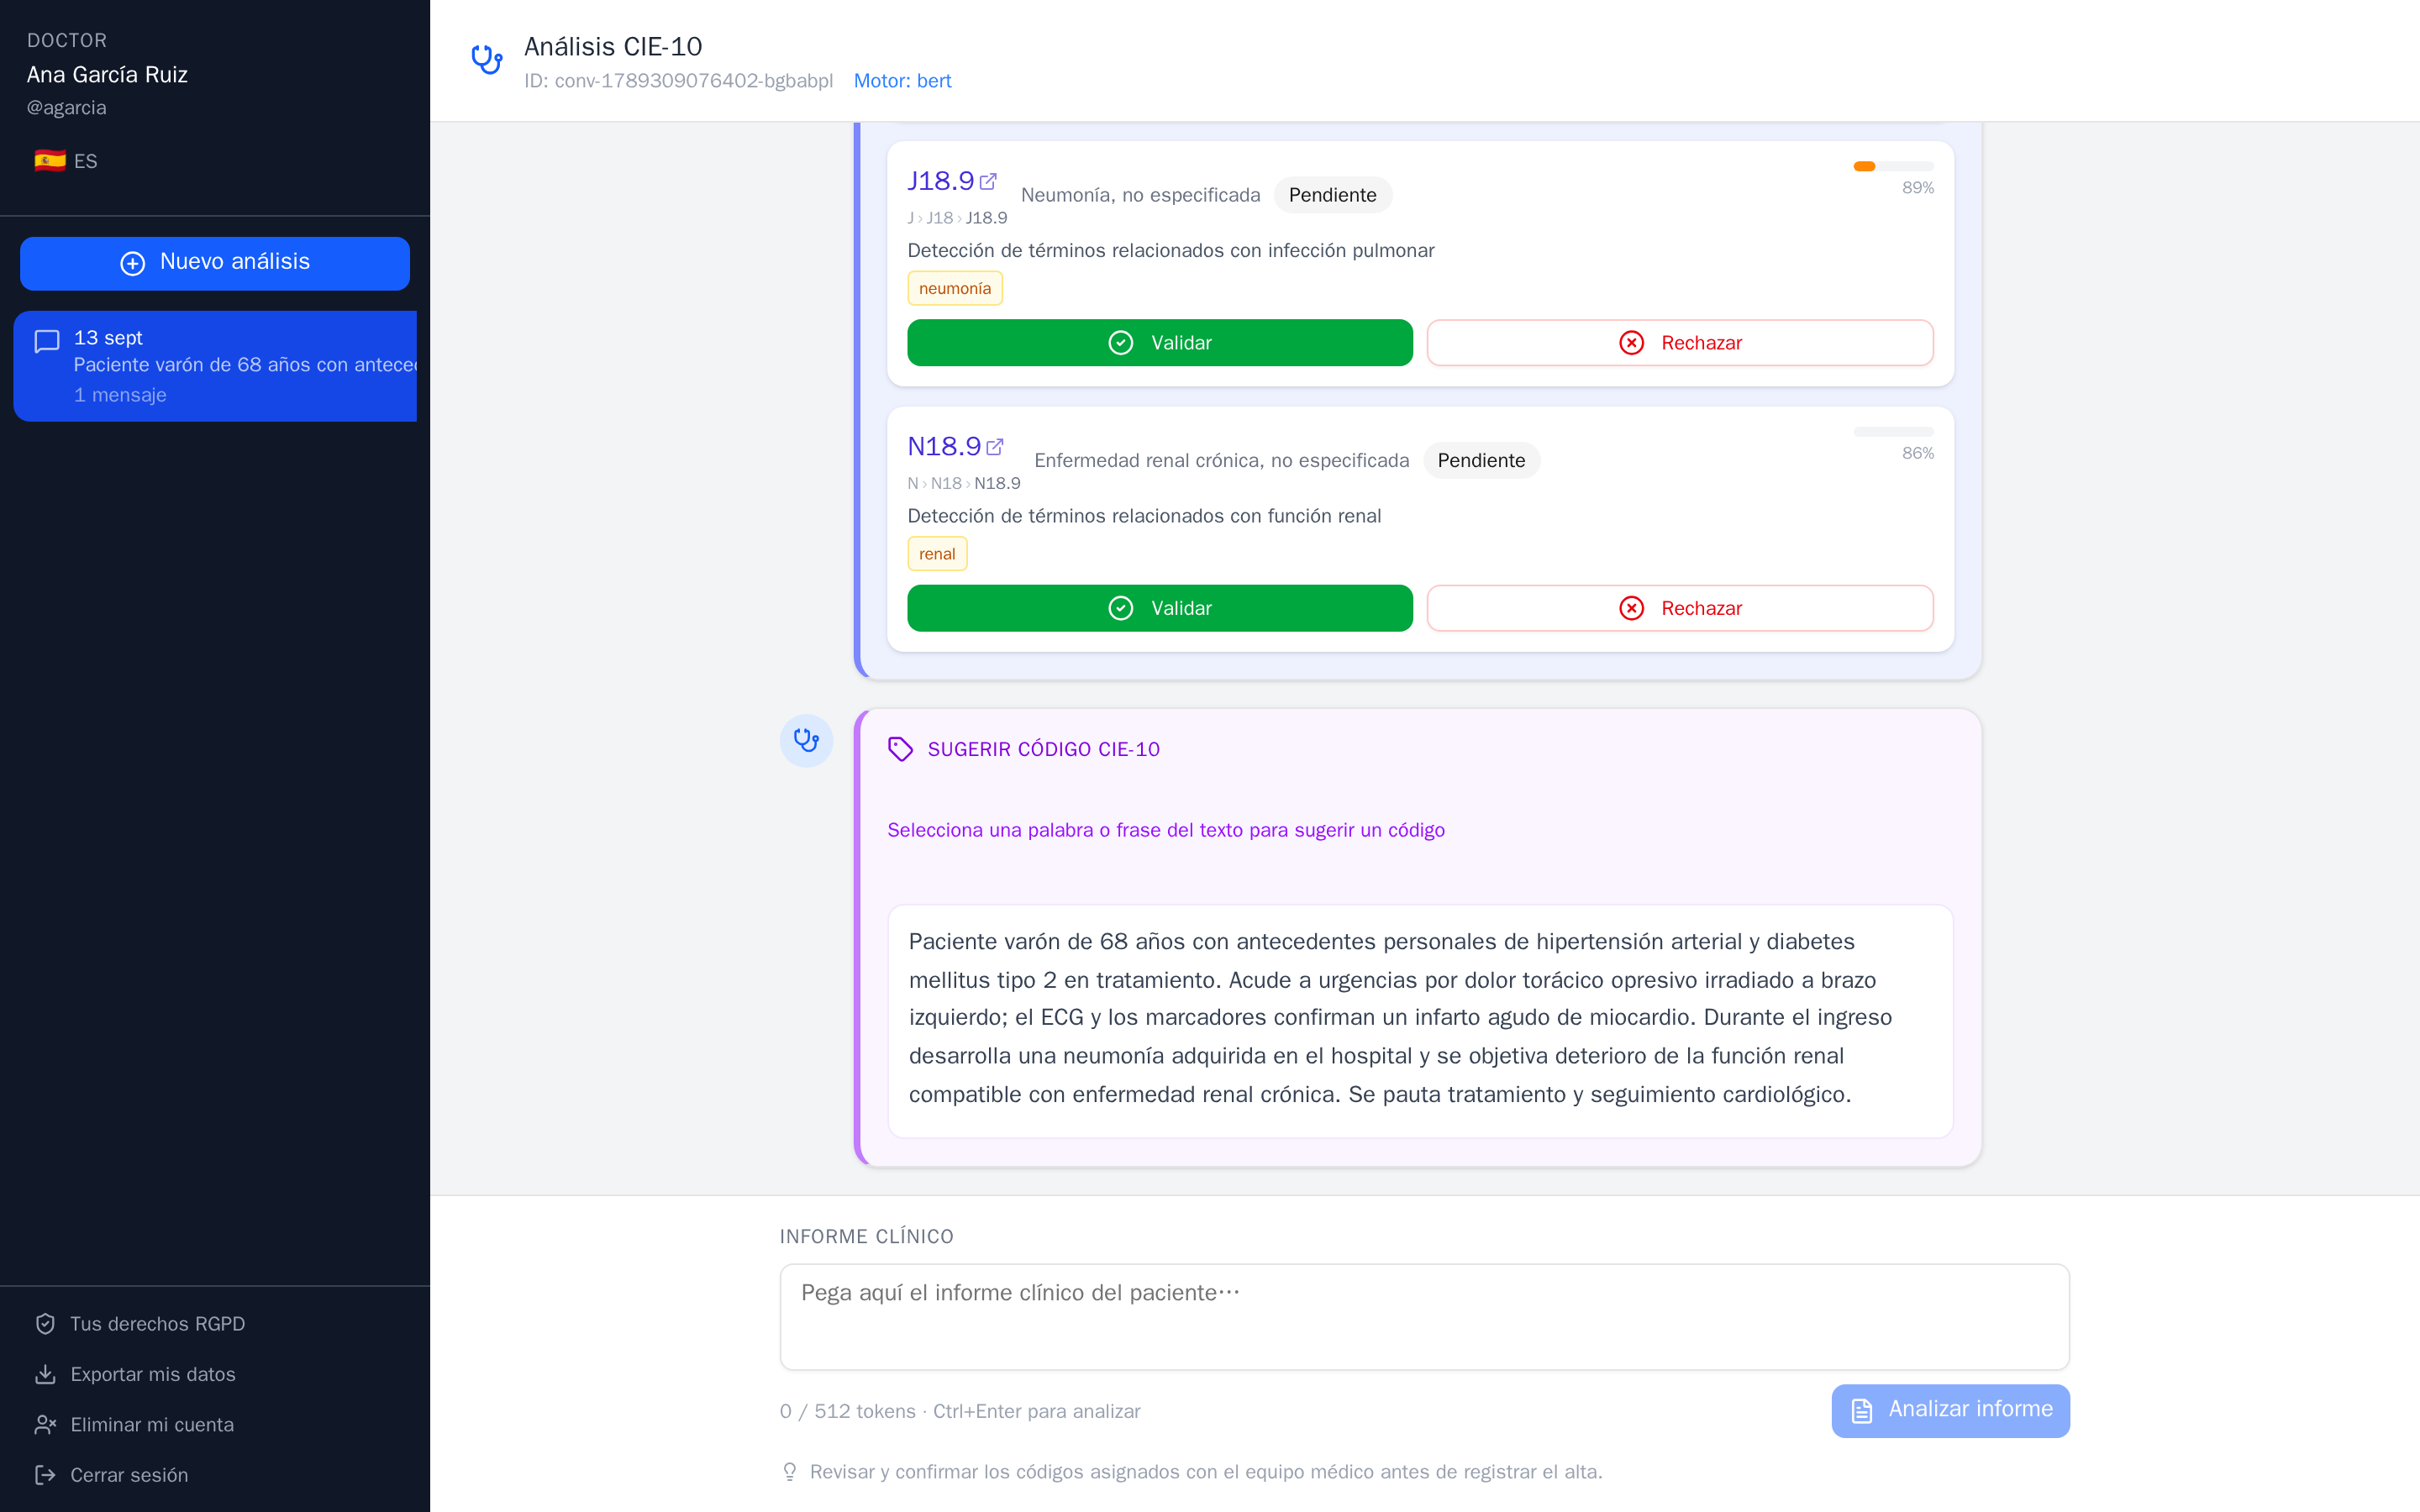
\includegraphics[width=0.8\textwidth, trim=920 0 360 130, clip]{figs/ui-analysis}
\caption{Área central de la interfaz web: tarjetas de códigos CIE-10 predichos, cada una con su nivel de confianza, los términos del informe que la motivan (\emph{chips} ámbar) y los controles de validación y rechazo, y el campo de entrada del informe. Se omite el panel lateral (historial y controles de sesión, incluidos los de RGPD), descrito en el texto.}
\label{fig:ui-analysis}
\end{figure}

\subsection{Requisitos}
\label{sec:requisitos}

A continuación se especifican los requisitos que debe cumplir el sistema, distinguiendo entre los funcionales, que describen qué debe hacer, y los no funcionales, que acotan cómo debe comportarse.

\subsubsection{Requisitos funcionales}

\begin{enumerate}[label=\textbf{RF\arabic*.}, leftmargin=*]
 \item \textbf{Entrada de datos:} Aceptar como entrada textos clínicos en español en formato libre, sin requerir marcado ni estructura predefinida.
 \item \textbf{Predicción de códigos:} Predecir uno o más códigos CIE-10-ES de diagnóstico para cada texto de entrada.
 \item \textbf{Puntuación de confianza:} Devolver una puntuación de confianza por cada código predicho, para priorizar la revisión humana de los casos de baja certeza.
 \item \textbf{Inferencia por lotes:} Admitir el procesamiento de múltiples textos de manera simultánea, devolviendo los resultados en el mismo orden que las entradas recibidas.
 \item \textbf{API REST:} Exponer las funcionalidades a través de una API REST documentada con al menos un endpoint de inferencia y uno de comprobación del estado del servicio.
\end{enumerate}

Los cinco anteriores acotan el motor de inteligencia artificial, que es el componente central. El sistema que se entrega, sin embargo, abarca los siete subobjetivos enumerados al principio del capítulo~\ref{cap:Objetivo}, de modo que los requisitos siguientes cubren las piezas restantes: el backend que orquesta el flujo, el módulo de resúmenes y la interfaz. Se enumeran aparte porque su verificación es de otra naturaleza, funcional y no métrica.

\begin{enumerate}[resume, label=\textbf{RF\arabic*.}, leftmargin=*]
 \item \textbf{Gestión de cuentas:} Permitir el alta de un usuario con verificación de la dirección de correo antes de conceder acceso, y autenticar las peticiones posteriores.
 \item \textbf{Orquestación del análisis:} Recibir un informe desde la interfaz, solicitar la predicción al motor y entregar los resultados de forma progresiva, sin que la parte más lenta del análisis retrase la aparición de los códigos.
 \item \textbf{Revisión de los códigos propuestos:} Permitir al codificador clínico validar o rechazar cada código, exigiendo un motivo en el rechazo, y conservar esas decisiones asociadas al análisis.
 \item \textbf{Resumen del informe:} Generar, mediante un modelo de lenguaje ejecutable en CPU, un resumen o paráfrasis del informe que se muestre junto a los códigos para agilizar la revisión.
 \item \textbf{Interfaz web:} Ofrecer una interfaz que permita enviar informes, seguir el análisis mientras se produce, consultar los términos que justifican cada código y recuperar los análisis anteriores.
\end{enumerate}

\subsubsection{Requisitos no funcionales}

\begin{enumerate}[label=\textbf{RNF\arabic*.}, leftmargin=*]
 \item \textbf{Rendimiento:} El sistema debe situarse dentro del rango de resultados de los sistemas participantes en el \emph{benchmark} CodiEsp~\cite{miranda2020}, que actúa como referencia, medido con la métrica oficial de la tarea (MAP por documento) sobre el mismo conjunto de prueba. Se considera cumplido si el sistema no queda por debajo del último de los sistemas participantes.
 \item \textbf{Latencia:} La propuesta de códigos debe completarse por debajo del segundo por informe en CPU de gama alta, de modo que el codificador clínico reciba los candidatos sin espera apreciable. La atribución de los términos que justifican cada código queda fuera de ese límite: es un orden de magnitud más cara, se sirve en una petición independiente y puede llegar después de los códigos, porque el usuario la consulta solo cuando despliega un código concreto.
 \item \textbf{Modularidad:} Los diferentes módulos del sistema deben tener interfaces bien definidas y ser sustituibles de forma independiente, de modo que, por ejemplo, el modelo base pueda cambiarse sin modificar el servicio de inferencia.
 \item \textbf{Trazabilidad:} El sistema debe registrar para cada predicción la versión del modelo empleada y el identificador del informe procesado, en línea con los principios de auditabilidad del Reglamento UE 2017/745~\cite{eu2017745} aplicable al software de apoyo a la decisión clínica.
 \item \textbf{Privacidad y protección de datos:} El tratamiento de los informes clínicos y de los datos de usuario debe ajustarse al Reglamento General de Protección de Datos (RGPD)~\cite{RGPD16}: minimización de datos, cifrado en tránsito y ejercicio de los derechos de supresión y portabilidad.
\end{enumerate}

\section{Diseño del sistema}

Esta sección describe el diseño del sistema de fuera hacia dentro: primero la arquitectura general de contenedores y sus interfaces, después el diseño del componente más crítico, el motor de inteligencia artificial (adquisición de datos, arquitectura del clasificador y proceso de entrenamiento), y por último el backend y el frontend que lo integran en un producto utilizable.

\subsection{Arquitectura general}

El sistema sigue una arquitectura orientada a servicios con cuatro capas bien diferenciadas: motor de inteligencia artificial, backend, frontend y capa de datos. Cada capa se despliega como un contenedor Docker independiente y se comunica con el resto a través de interfaces explícitas, lo que permite actualizar o sustituir cualquier componente sin afectar al resto del sistema.

El \textbf{frontend} (Next.js, React 19) se comunica con el \textbf{backend} (Elixir, Phoenix 1.8) mediante dos canales: una API REST para operaciones de autenticación y consulta, y un canal WebSocket para la recepción de tarjetas de análisis en tiempo real. El backend actúa como orquestador central: recibe los informes clínicos del usuario, los envía al \textbf{motor de IA} (Python, FastAPI) a través de una llamada HTTP síncrona, y retransmite las predicciones resultantes al cliente a medida que se generan. La \textbf{base de datos} PostgreSQL almacena tanto el registro de eventos inmutable del \emph{event store} como las proyecciones de lectura actualizadas por los proyectores del backend.

Dos decisiones arquitectónicas clave vertebran el diseño. Por un lado, el patrón CQRS/\emph{Event Sourcing} en el backend proporciona trazabilidad de las acciones clínicas sobre cada análisis. Por otro lado, el motor de IA se mantiene como servicio independiente, lo que permite actualizar el modelo BERT sin recompilar ni reiniciar el resto del sistema. Para describir la arquitectura en detalle se emplea el modelo C4~\cite{Brown22}. La topología completa de contenedores, puertos y variables de entorno se amplía en el Anexo~\ref{cap:AnexoB}; los contratos de comunicación entre servicios, en el Anexo~\ref{cap:AnexoC}; el esquema de base de datos, en el Anexo~\ref{cap:AnexoD}; y las decisiones de diseño que justifican las elecciones tecnológicas, en el Anexo~\ref{cap:AnexoE}.

\textbf{Nivel de contexto.} El sistema recibe informes clínicos en texto libre de parte del codificador clínico y devuelve propuestas de codificación CIE-10-ES. Se comunica con el portal eCIE-maps del Ministerio de Sanidad como fuente de datos externa (en la fase de adquisición de datos).

\textbf{Nivel de contenedores.} El sistema se compone de cuatro contenedores:

\begin{enumerate}
 \item \textbf{Frontend} (Next.js 16, TypeScript): interfaz web que el usuario utiliza para enviar informes y visualizar resultados. Se comunica con el backend mediante una API REST para autenticación y con un canal WebSocket para el intercambio de mensajes en tiempo real.
 \item \textbf{Backend} (Elixir 1.19, Phoenix 1.8): orquestador central del sistema. Gestiona la autenticación de usuarios, la persistencia de conversaciones mediante CQRS/Event Sourcing con la biblioteca Commanded y la comunicación con el motor de IA.
 \item \textbf{AI Engine} (Python, FastAPI): servicio de inferencia que carga el modelo BERT entrenado y expone un endpoint \texttt{POST /predict} que recibe un texto clínico y devuelve los códigos CIE-10-ES predichos con sus puntuaciones de confianza.
 \item \textbf{Base de datos} (PostgreSQL 18): almacena usuarios, conversaciones, tarjetas de análisis y el registro de eventos del sistema (event store de Commanded).
\end{enumerate}

\subsection{Diseño del motor de inteligencia artificial}

El motor de IA es el componente más crítico del sistema. Su diseño pasa por tres fases: adquisición de datos, entrenamiento del modelo y exposición del servicio de inferencia.

\subsubsection{Adquisición de datos}
\label{sec:adquisicion}

El sistema requiere dos fuentes de datos complementarias: el corpus de informes clínicos anotados (CodiEsp) y el catálogo oficial de códigos CIE-10-ES con sus descripciones en español. La Figura~\ref{fig:pipeline-datos} resume el flujo completo, desde la adquisición hasta el entrenamiento.

\begin{figure}[ht]
\centering
\resizebox{\textwidth}{!}{
\begin{tikzpicture}[
  every node/.style={font=\normalsize\sffamily},
  src/.style={draw=palered!80, fill=palered!10, thick, rectangle, rounded corners=3pt,
              minimum width=2.8cm, minimum height=1.1cm, align=center},
  csvn/.style={draw=black!60, fill=gray!10, thick, rectangle, rounded corners=3pt,
               minimum width=3.4cm, minimum height=1.1cm, align=center},
  proc/.style={draw=aquaESI!80, fill=aquaESI!15, thick, rectangle, rounded corners=3pt,
               minimum width=3.2cm, minimum height=1.3cm, align=center},
  fin/.style={draw=ocre!80, fill=ocre!15, thick, rectangle, rounded corners=3pt,
              minimum width=3.0cm, minimum height=1.3cm, align=center},
  arr/.style={->, >=Stealth, thick},
]
\node[src] (ecie) at (0,1.3) {eCIE-maps};
\node[src] (codi) at (0,-1.3) {CodiEsp};
\node[csvn] (ccsv) at (4.6,1.3) {\texttt{cie10-*.csv}};
\node[csvn] (dcsv) at (4.6,-1.3) {\texttt{codiesp\_*.csv}};
\node[proc] (pre) at (9.4,0) {Preprocesado y\\particiones};
\node[fin] (trn) at (13.8,0) {Entrenamiento};

\draw[arr] (ecie) -- (ccsv);
\draw[arr] (codi) -- (dcsv);
\draw[arr] (ccsv) -- (pre);
\draw[arr] (dcsv) -- (pre);
\draw[arr] (pre) -- (trn);
\end{tikzpicture}
}
\caption{Flujo de datos del sistema: adquisición de las dos fuentes (catálogo CIE-10-ES por \emph{scraping} de eCIE-maps y corpus CodiEsp), generación de los CSV, preprocesado al formato multilabel, partición en train/val/test y entrenamiento.}
\label{fig:pipeline-datos}
\end{figure}

\paragraph{Corpus CodiEsp.}
El corpus CodiEsp~\cite{miranda2020} fue creado en el contexto de la tarea compartida CodiEsp de CLEF eHealth 2020 y constituye un recurso público de referencia para la codificación automática de textos clínicos en español. Contiene 1.000 casos clínicos publicados, escritos en español y de diversas especialidades médicas, anotados manualmente por codificadores profesionales con los códigos CIE-10-ES correspondientes, distribuidos en tres particiones:

\begin{itemize}
 \item \textbf{Entrenamiento:} 500 documentos (50\,\%).
 \item \textbf{Validación:} 250 documentos (25\,\%).
 \item \textbf{Test:} 250 documentos (25\,\%).
\end{itemize}

La adquisición se realizó mediante el script \texttt{collect\_codiesp\_dataset.py}, que descarga los ficheros de diagnósticos (sufijo \texttt{\_D\_}), procedimientos (\texttt{\_P\_}) y la variante extendida con anotaciones a nivel de \emph{span} (\texttt{\_X\_}), normaliza la codificación de caracteres y genera los ficheros CSV empleados en las fases de entrenamiento y evaluación.

\paragraph{Catálogo CIE-10-ES mediante \emph{scraping} del portal eCIE-maps.}
El diccionario oficial CIE-10-ES no está disponible en ningún formato de descarga pública estructurada. La única fuente oficial es el portal eCIE-maps del Ministerio de Sanidad (\texttt{www.eciemaps.sanidad.gob.es}), que expone los datos a través de una API web no documentada. Para obtener el catálogo completo se analizó el tráfico de red del portal identificando el patrón de los \emph{endpoints} REST que sirven los datos en formato JSON, y se desarrollaron tres scripts de extracción:

\begin{itemize}
 \item \texttt{collect\_diagnoses.py}: itera sobre las 260 combinaciones letra–dígito del \emph{endpoint} de diagnósticos mediante peticiones asíncronas con \texttt{grequests}. Genera \texttt{cie10-es-diagnoses.csv} con \textbf{101.246 registros}.
 \item \texttt{collect\_procedures.py}: recorre la jerarquía de tres niveles de procedimientos (secciones, subsecciones y tablas). Genera \texttt{cie10-es-procedures.csv} con \textbf{78.496 registros}.
 \item \texttt{collect\_chemicals.py}: recorre las 27 letras del índice de fármacos. Genera \texttt{cie10-es-\allowbreak{}chemicals.csv} con \textbf{5.050 registros}.
\end{itemize}

Tres factores técnicos fueron determinantes para el éxito de la extracción: la simulación de cabeceras HTTP de navegador (\texttt{User-Agent}, \texttt{Accept}, \texttt{Referer}) para evitar respuestas 403, el paralelismo con reintentos automáticos para garantizar la integridad del catálogo, y el procesamiento por lotes para evitar el agotamiento de memoria en el volumen de procedimientos. Cada entrada incluye el código, la descripción en español y metadatos clínicos (restricciones de sexo, edad perinatal/pediátrica/materna/adulta, exención de POA y prohibición como diagnóstico principal).

\subsubsection{Análisis exploratorio de los datos}
\label{sec:analisis_datos}

Antes de diseñar el modelo se realizó un análisis estadístico exhaustivo de ambas fuentes, documentado en los notebooks \texttt{codiesp\_analisis\_estadistico.ipynb} y\linebreak \texttt{cie10\_analisis\_estadistico.ipynb}.

\paragraph{Longitud de los textos clínicos.}
Los informes tienen una longitud media de 2.317 caracteres (349 palabras) en el conjunto de entrenamiento, con desviación estándar de 1.097 caracteres y rango entre 556 y 7.466 caracteres. La distribución es aproximadamente log-normal. Aplicando el tokenizador de RigoBERTa-Clinical se comprobó que el \textbf{53,6\,\% de los documentos de entrenamiento supera los 512 tokens} (máximo: 1.888 tokens) y que el \textbf{100\,\% queda por debajo de 2.048 tokens}, con una distribución prácticamente idéntica en validación y prueba (58\,\% supera los 512 tokens en ambas). Aunque más de la mitad de los informes se trunca a 512 tokens, los experimentos con ventanas más largas (sección~\ref{sec:entrenamiento}) no mejoraron el resultado, lo que es compatible con que buena parte de la información diagnóstica se concentre en esos primeros 512 tokens, aunque no se midió directamente. Esos resultados fundamentan la elección de \texttt{max\_length}=512 y el descarte de la ventana deslizante (Figura~\ref{fig:tokens}).

\begin{figure}[ht]
\centering
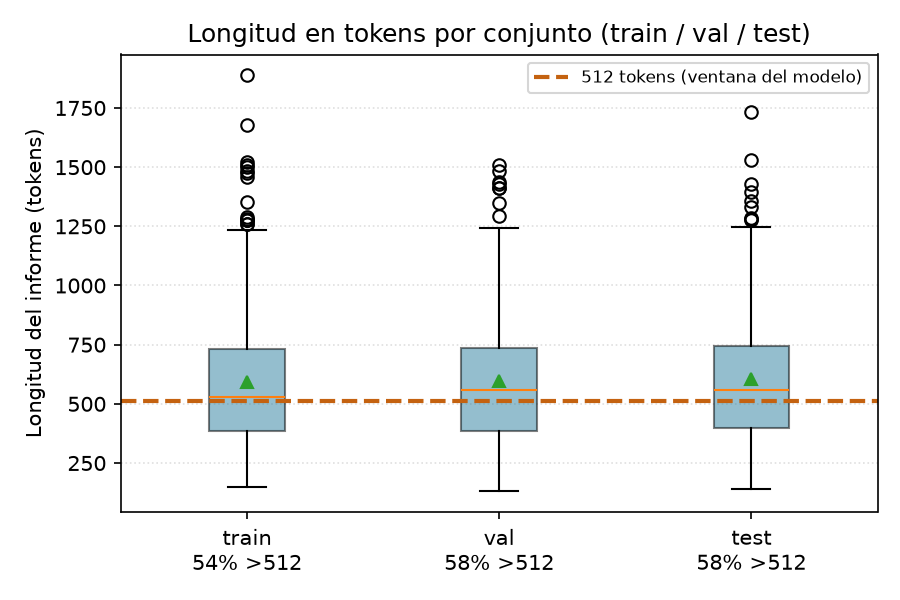
\includegraphics[width=0.72\textwidth]{figs/tfg_tokens}
\caption[Longitud de los informes en \emph{tokens} por conjunto (train/val/test)]{Longitud de los informes en \emph{tokens} por conjunto (train/val/test). Más de la mitad supera los 512 \emph{tokens} de la ventana del modelo (54\,\% en entrenamiento, 58\,\% en validación y prueba), pero la totalidad queda por debajo de 2.048. La distribución es homogénea entre los tres conjuntos.}
\label{fig:tokens}
\end{figure}

\paragraph{Distribución de etiquetas.}
Cada documento tiene una media de 11,3 códigos CIE-10-ES asignados (mediana: 10; máximo: 40; mínimo: 1). La correlación entre longitud del texto y número de etiquetas es de 0,56. La distribución de frecuencias sigue una ley de potencia: la mayoría de los 2.557 códigos únicos del corpus aparece en cinco o menos documentos. Esta distribución de cola larga motivó el uso de ponderación de clases en la función de pérdida (Figura~\ref{fig:longtail}).

\begin{figure}[ht]
\centering
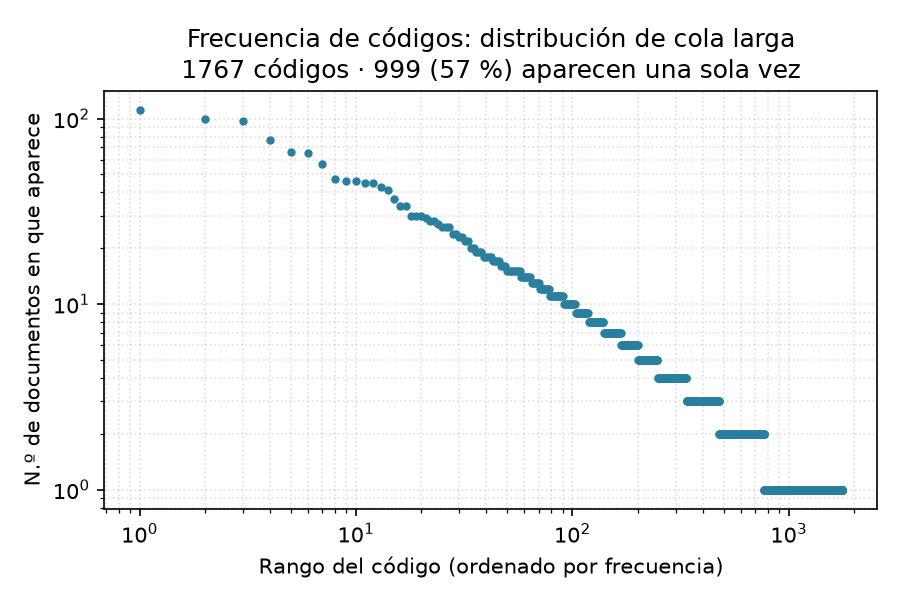
\includegraphics[width=0.72\textwidth]{figs/tfg_longtail}
\caption{Distribución de frecuencias de los códigos en el conjunto de entrenamiento (escala log-log): una minoría de códigos concentra la mayoría de las apariciones y más de la mitad aparece una sola vez, lo que motiva la ponderación de clases y el preentrenamiento.}
\label{fig:longtail}
\end{figure}

\paragraph{Solapamiento entre particiones.}
El coeficiente de Jaccard entre particiones se sitúa entre 0,31 y 0,33. El dato más relevante para la evaluación es que \textbf{el 38\,\% de los códigos distintos del conjunto de prueba (439 de 1.143, Tabla~\ref{tab:jaccard} del Anexo~\ref{cap:AnexoG}) no aparece en ningún documento de entrenamiento}, lo que impone un techo teórico al F1-macro independiente de la arquitectura elegida.

\paragraph{Características del catálogo CIE-10-ES.}
El catálogo contiene 101.246 entradas en 21 capítulos. Esta cifra supera los 68.069 códigos válidos de la CIE-10-ES~\cite{sanidad2016cie10} mencionados en la introducción porque el navegador eCIE-maps expone \emph{todos} los nodos del árbol jerárquico, incluidas las categorías de tres caracteres y las subcategorías intermedias, que no son códigos facturables finales; además, muchas entradas agrupan variantes o sinónimos de una misma descripción. Las categorías más representadas son R (síntomas y signos), S (traumatismos), T (envenenamientos) e I (enfermedades circulatorias). Esta distribución, unida a que solo una fracción de los códigos aparece en CodiEsp, explica que el espacio de clases del clasificador se limite a los 1.767 códigos completos (p.\,ej.\ \texttt{E11.9}) únicos del conjunto de entrenamiento, frente a los más de 100.000 del catálogo CIE-10-ES.

\paragraph{Brecha léxica entre catálogo oficial y lenguaje clínico real.}
El análisis lingüístico realizado con SpaCy (modelo \texttt{es\_core\_news\_lg}) sobre las descripciones del catálogo CIE-10-ES reveló que el vocabulario oficial emplea 10.874 lemas únicos, dominado por sustantivos técnicos (47,3\,\%) y adjetivos específicos (29,6\,\%). La validación cruzada de este vocabulario con los informes clínicos del corpus CodiEsp, documentada en el \emph{notebook} \texttt{cie10\_spacy\_word\_analysis.ipynb}, arrojó un resultado clínicamente significativo: \textbf{solo el 38,3\,\% de los lemas del catálogo oficial aparece en los textos de los informes clínicos del corpus}. Los 6.708 lemas restantes pertenecen a la nomenclatura estandarizada, pero no forman parte del lenguaje habitual con que se redactan los casos clínicos.

Esta brecha tiene una causa directa en la práctica clínica: el catálogo CIE-10 emplea denominaciones largas y normalizadas («infarto agudo de miocardio de cara anterior de transmisión transmural»), mientras que el médico redacta con abreviaturas frecuentes (\texttt{IAM}, \texttt{EPOC}, \texttt{HTA}, \texttt{DM2}), epónimos y expresiones propias del entorno hospitalario. El análisis identificó además un 44,4\,\% de lemas con especificidad máxima, asociados a un único código CIE-10, frente a términos de alta dispersión como «contacto», «fractura» o «especificado», que aparecen en miles de códigos diferentes. Esta estructura léxica justifica dos decisiones de diseño que se desarrollan en las secciones siguientes: (1) la elección de un \emph{encoder} preentrenado en texto clínico en español (RigoBERTa-Clinical), que ha aprendido a relacionar las expresiones del lenguaje médico real con las denominaciones de los diagnósticos sin depender de coincidencia léxica exacta; y (2) la expansión de abreviaturas clínicas implementada en el clasificador de diccionario, que normaliza expresiones habituales antes de la búsqueda en el catálogo. El análisis detallado del vocabulario se recoge en el Anexo~\ref{cap:AnexoG}.

\subsubsection{Métricas de evaluación}
\label{sec:metricas}

Las métricas se definen sobre el vocabulario $C$ del modelo (1.767 códigos) y un conjunto de documentos $D$. Para cada documento $d$ y código $c$, $y_{dc}\in\{0,1\}$ indica si $c$ figura en la anotación de referencia (\emph{gold}) y $\hat{y}_{dc}\in\{0,1\}$ si el sistema lo propone, es decir, si su probabilidad alcanza el umbral $\tau$. Por código, $TP_c=\sum_d y_{dc}\hat{y}_{dc}$, $FP_c=\sum_d (1-y_{dc})\hat{y}_{dc}$ y $FN_c=\sum_d y_{dc}(1-\hat{y}_{dc})$.

\paragraph{F1-micro y F1-macro.} El F1-micro agrupa todos los pares (documento, código), de modo que cada código pesa según su frecuencia:
\begin{equation}
P_{\mu}=\frac{\sum_c TP_c}{\sum_c (TP_c+FP_c)},\qquad R_{\mu}=\frac{\sum_c TP_c}{\sum_c (TP_c+FN_c)},\qquad F1_{\mu}=\frac{2\,P_{\mu}R_{\mu}}{P_{\mu}+R_{\mu}}.
\end{equation}
El F1-macro calcula el F1 de cada código y promedia sin ponderar:
\begin{equation}
F1_c=\frac{2\,TP_c}{2\,TP_c+FP_c+FN_c},\qquad F1_{M}=\frac{1}{|C|}\sum_{c\in C}F1_c,
\end{equation}
con $F1_c=0$ cuando el código no aparece ni en la referencia ni en las predicciones. Como el promedio recorre los 1.767 códigos, los poco frecuentes pesan tanto como los comunes y los que no tienen ejemplos en prueba cuentan como cero, lo que explica en parte la brecha entre F1-micro y F1-macro.

\paragraph{MAP por documento.} Para un documento $d$ se ordenan los códigos de $C$ por probabilidad decreciente (por puntuación fusionada en el modo fusionado) y se promedia la precisión en las posiciones donde aparece un código de la referencia:
\begin{equation}
AP_d=\frac{1}{n_d}\sum_{k=1}^{|C|}P_d@k\cdot rel_d(k),\qquad MAP=\frac{1}{|D'|}\sum_{d\in D'}AP_d,
\end{equation}
donde $P_d@k$ es la precisión de las $k$ primeras posiciones, $rel_d(k)=1$ si el código en la posición $k$ pertenece a la referencia y $n_d$ es el número de códigos de la referencia de $d$. A diferencia del F1, no depende del umbral: mide el orden, no la decisión. Con el mismo cálculo hay dos variantes, según el denominador. En el \emph{MAP estricto}, $n_d$ cuenta todos los códigos de la referencia, también los que están fuera del vocabulario del modelo, que nunca se pueden proponer y penalizan el resultado, y $D'$ son los documentos con al menos un código de referencia; es el comparable con el \emph{benchmark}. En el \emph{MAP alcanzable}, $n_d$ cuenta solo los códigos de la referencia que pertenecen al vocabulario y $D'$ los documentos con al menos uno; es una cota superior y no es comparable con otros sistemas. Las tres métricas se calculan en \texttt{ai\_engine/\allowbreak{}eval\_test.py} (\texttt{make ai-eval-test}).

\subsubsection{Selección del modelo base}

Se evaluaron diez modelos candidatos para la codificación del texto clínico. La comparativa, recogida en el Anexo~\ref{cap:AnexoA}, consideró rendimiento en CodiEsp, especialización en español médico, velocidad de inferencia y coste computacional de entrenamiento. Los modelos evaluados fueron:

\begin{itemize}
 \item \texttt{PlanTL-GOB-ES/roberta-base-biomedical-clinical-es} (RoBERTa-BSC, 125M parámetros), entrenado por el Barcelona Supercomputing Center sobre historias clínicas, informes radiológicos y notas médicas en español.
 \item \texttt{PlanTL-GOB-ES/roberta-large-bne} (355M parámetros), variante de mayor tamaño del mismo grupo (deprecado; referencia de escala).
 \item Longformer-BSC (\texttt{PlanTL-GOB-ES/\allowbreak{}longformer-base-4096-\allowbreak{}biomedical-clinical-es}, $\sim$130M parámetros, ventana de 4.096 tokens), variante del modelo clínico del Barcelona Supercomputing Center con atención dispersa para secuencias largas.
 \item \texttt{IIC/RigoBERTa-2.0} (arquitectura XLM-RoBERTa-large, $\sim$600M parámetros), versión de propósito general desarrollada por el Instituto de Ingeniería del Conocimiento sobre corpus español de gran escala.
 \item \texttt{IIC/RigoBERTa-Clinical} (XLM-RoBERTa-large, especialización clínica), variante de RigoBERTa entrenada sobre corpus médico en español por el Instituto de Ingeniería del Conocimiento; modelo seleccionado para el entrenamiento final en producción.
 \item \texttt{jhu-clsp/mmBERT-base} (mmBERT, arquitectura ModernBERT multilingüe), modelo con ventana de 8.192 tokens entrenado sobre 1800+ lenguas, desarrollado por el Centro de Procesamiento del Lenguaje y del Habla de la Universidad Johns Hopkins.
 \item \texttt{answerdotai/ModernBERT-base} (ModernBERT, 2024), arquitectura de última generación con Flash Attention y ventana de 8.192 tokens; obtuvo un F1-micro de 0{,}632 en pruebas de nivel~1.
 \item \texttt{dccuchile/bert-base-spanish-wwm-cased} (BETO, 110M parámetros), modelo de propósito general en español.
 \item \texttt{sentence-transformers/paraphrase-multilingual-MiniLM-L12-v2} (33M parámetros), orientado a la generación de embeddings.
 \item \texttt{distilbert-base-multilingual-cased} (66M parámetros), versión destilada multilingüe de BERT.
\end{itemize}

El modelo seleccionado como base fue \texttt{IIC/RigoBERTa-Clinical} para el entrenamiento final en producción, dado que combina la especialización en dominio clínico español con la mayor capacidad del grupo de modelos evaluados (XLM-RoBERTa-large, $\sim$600M parámetros) y obtuvo un F1-micro de 0{,}761 en la tarea de clasificación de capítulos, a dos puntos del mejor candidato y dentro de la dispersión entre ejecuciones. Para pruebas rápidas se usa \texttt{roberta-base} como alternativa más ligera.

\subsubsection{Arquitectura del clasificador}

El clasificador sigue una arquitectura plana (\emph{flat}) de clasificación multilabel. La entrada es el texto del informe clínico codificado por el tokenizador del modelo base; la salida es un vector de probabilidades de dimensión igual al número de códigos presentes en el corpus de entrenamiento (aproximadamente 1.767 códigos únicos en la partición de diagnósticos de CodiEsp).

Sobre el \emph{encoder} BERT se añade una cabeza de clasificación compuesta por una capa de \emph{dropout} (p\,=\,0,3 en producción) y una capa lineal que proyecta la representación del token \texttt{[CLS]} al espacio de códigos. La activación utilizada en inferencia es una sigmoide por código, de modo que cada predicción es independiente del resto y el modelo puede asignar simultáneamente cualquier subconjunto de códigos. Durante el entrenamiento se utiliza \emph{Binary Cross-Entropy} como función de pérdida. La planificación de la tasa de aprendizaje se determinó experimentalmente: la configuración de producción emplea un \emph{scheduler} de tipo \emph{plateau}, que resultó superior al \emph{cosine schedule with warmup} inicial (sección~\ref{sec:entrenamiento}).

La Figura~\ref{fig:arq-clasificador} resume esta arquitectura, del informe clínico a los códigos predichos.

\begin{figure}[ht]
\centering
\resizebox{\textwidth}{!}{% Arquitectura del clasificador plano multilabel CIE-10
% Uso: % Arquitectura del clasificador plano multilabel CIE-10
% Uso: \input{figs/arq-clasificador} dentro de figure+\centering+\resizebox{\textwidth}{!}{...}
% Flujo: informe → tokenizador → encoder RigoBERTa-Clinical → [CLS] → dropout → lineal → sigmoide → umbral

\begin{tikzpicture}[
  every node/.style={font=\small\sffamily},
  io/.style={draw=palered!80, fill=palered!10, thick, rectangle, rounded corners=3pt,
             minimum width=2.1cm, minimum height=1.0cm, align=center},
  enc/.style={draw=aquaESI!80, fill=aquaESI!15, thick, rectangle, rounded corners=3pt,
              minimum width=3.0cm, minimum height=1.7cm, align=center},
  blk/.style={draw=gray!60, fill=gray!10, thick, rectangle, rounded corners=3pt,
              minimum width=1.9cm, minimum height=1.0cm, align=center},
  res/.style={draw=ocre!80, fill=ocre!18, thick, rectangle, rounded corners=3pt,
              minimum width=2.1cm, minimum height=1.0cm, align=center},
  arr/.style={->, >=Stealth, thick},
  node distance=0.65cm
]

\node[io] (inp) {Informe\\clínico};
\node[blk, right=of inp] (tok) {Tokenizador\\\scriptsize $\leq$512 tokens};
\node[enc, right=of tok] (enc) {\textbf{Encoder}\\RigoBERTa-Clinical\\\scriptsize XLM-R-large, 24 capas\\\scriptsize freeze=20 (4 entrenables)};
\node[blk, right=of enc] (cls) {token [CLS]\\\scriptsize 1024-d};
\node[blk, right=of cls] (drp) {Dropout\\\scriptsize 0,3};
\node[blk, right=of drp] (lin) {Capa lineal\\\scriptsize 1024$\to$1767};
\node[res, right=of lin] (sig) {Sigmoide\\\scriptsize por código};
\node[res, right=of sig] (thr) {Umbral 0,3\\\scriptsize $\to$ códigos};

\draw[arr] (inp) -- (tok);
\draw[arr] (tok) -- (enc);
\draw[arr] (enc) -- (cls);
\draw[arr] (cls) -- (drp);
\draw[arr] (drp) -- (lin);
\draw[arr] (lin) -- (sig);
\draw[arr] (sig) -- (thr);

% Nota: preentrenamiento débil antes del fine-tuning
\node[draw=turquesa!70, fill=turquesa!12, thick, rectangle, rounded corners=3pt,
      align=center, font=\scriptsize\sffamily, below=1.1cm of enc, text width=4.6cm]
      (pre) {\textbf{Preentrenamiento débil}\\descripciones CIE-10-ES + \emph{snippets} del task\_X\\$\rightarrow$ \emph{fine-tuning} sobre CodiEsp};
\draw[arr, turquesa!80, dashed] (pre) -- (enc);

\end{tikzpicture}
 dentro de figure+\centering+\resizebox{\textwidth}{!}{...}
% Flujo: informe → tokenizador → encoder RigoBERTa-Clinical → [CLS] → dropout → lineal → sigmoide → umbral

\begin{tikzpicture}[
  every node/.style={font=\small\sffamily},
  io/.style={draw=palered!80, fill=palered!10, thick, rectangle, rounded corners=3pt,
             minimum width=2.1cm, minimum height=1.0cm, align=center},
  enc/.style={draw=aquaESI!80, fill=aquaESI!15, thick, rectangle, rounded corners=3pt,
              minimum width=3.0cm, minimum height=1.7cm, align=center},
  blk/.style={draw=gray!60, fill=gray!10, thick, rectangle, rounded corners=3pt,
              minimum width=1.9cm, minimum height=1.0cm, align=center},
  res/.style={draw=ocre!80, fill=ocre!18, thick, rectangle, rounded corners=3pt,
              minimum width=2.1cm, minimum height=1.0cm, align=center},
  arr/.style={->, >=Stealth, thick},
  node distance=0.65cm
]

\node[io] (inp) {Informe\\clínico};
\node[blk, right=of inp] (tok) {Tokenizador\\\scriptsize $\leq$512 tokens};
\node[enc, right=of tok] (enc) {\textbf{Encoder}\\RigoBERTa-Clinical\\\scriptsize XLM-R-large, 24 capas\\\scriptsize freeze=20 (4 entrenables)};
\node[blk, right=of enc] (cls) {token [CLS]\\\scriptsize 1024-d};
\node[blk, right=of cls] (drp) {Dropout\\\scriptsize 0,3};
\node[blk, right=of drp] (lin) {Capa lineal\\\scriptsize 1024$\to$1767};
\node[res, right=of lin] (sig) {Sigmoide\\\scriptsize por código};
\node[res, right=of sig] (thr) {Umbral 0,3\\\scriptsize $\to$ códigos};

\draw[arr] (inp) -- (tok);
\draw[arr] (tok) -- (enc);
\draw[arr] (enc) -- (cls);
\draw[arr] (cls) -- (drp);
\draw[arr] (drp) -- (lin);
\draw[arr] (lin) -- (sig);
\draw[arr] (sig) -- (thr);

% Nota: preentrenamiento débil antes del fine-tuning
\node[draw=turquesa!70, fill=turquesa!12, thick, rectangle, rounded corners=3pt,
      align=center, font=\scriptsize\sffamily, below=1.1cm of enc, text width=4.6cm]
      (pre) {\textbf{Preentrenamiento débil}\\descripciones CIE-10-ES + \emph{snippets} del task\_X\\$\rightarrow$ \emph{fine-tuning} sobre CodiEsp};
\draw[arr, turquesa!80, dashed] (pre) -- (enc);

\end{tikzpicture}
}
\caption{Arquitectura del clasificador plano multilabel: el \emph{encoder} RigoBERTa-Clinical (preentrenado de forma débil sobre el catálogo CIE-10-ES antes del \emph{fine-tuning}) proyecta la representación del token \texttt{[CLS]} sobre los 1.767 códigos mediante una cabeza lineal con activación sigmoide por código.}
\label{fig:arq-clasificador}
\end{figure}

La selección de los códigos predichos se realiza mediante un umbral sobre la probabilidad, 0,2 en la configuración de producción, seleccionado mediante barrido en validación (sección~\ref{sec:entrenamiento}); el servicio lo lee del fichero \texttt{config.json} generado durante el entrenamiento. El servicio devuelve como máximo los diez códigos de mayor probabilidad que superan el umbral (el límite está fijado en el código del servicio, no en \texttt{config.json}) y, si ninguno lo supera, la lista queda vacía.

\paragraph{FlashAttention~2: implementación eficiente del mecanismo de atención.}
El \emph{encoder} de RigoBERTa-Clinical utiliza FlashAttention~2~\cite{dao2023flashattention2} en lugar de la implementación estándar de auto-atención de PyTorch. FlashAttention~2 reordena el cómputo de la atención para reducir el consumo de memoria y acelerar cada paso sin alterar el resultado en aritmética exacta. Sobre la tarea de capítulos y la máquina de desarrollo (RTX 4080), la mediana por época baja de 11,9~s con la implementación \texttt{sdpa} de PyTorch a 9,9~s con FlashAttention~2, un 17\,\% menos. Conviene matizar esa última afirmación, porque el entrenamiento se realiza en \texttt{bfloat16}: el reordenamiento cambia el orden de acumulación y, con esa precisión, el resultado no es bit a bit idéntico. En cuanto al resultado, esa misma comprobación da 0,748 con \texttt{sdpa} frente a 0,757 y 0,764 con FlashAttention~2, una diferencia del mismo orden que la dispersión entre ejecuciones con la misma configuración, de modo que no cabe atribuirle un efecto sistemático.

Lo que sí tiene consecuencias es cómo se elige la implementación. Los cuadernos la seleccionaban en función de si la biblioteca estaba instalada en la imagen, lo que hacía que el mismo código diera resultados distintos en entornos distintos sin que nada lo indicara. Se fija ahora de forma explícita mediante el parámetro \texttt{ATTN\_IMPL} de la configuración de los cuadernos, que es condición necesaria para que una ejecución sea reproducible: una dependencia presente o ausente no debe decidir en silencio cómo se entrena el modelo.

\paragraph{Clasificador de diccionario (\texttt{baseline\_dict.py}).}
\label{sec:diccionario}
El motor de IA incluye un clasificador de diccionario que actúa como \textbf{complemento determinista} de RigoBERTa-Clinical, no como alternativa. Cumple tres funciones: sirve de \emph{baseline} de referencia para evaluar el valor añadido del modelo neuronal, actúa de \emph{fallback} cuando el modelo BERT no está disponible en producción, y puede combinarse con las predicciones neurales a través del parámetro \texttt{engine=\textquotedbl{}both\textquotedbl{}} del endpoint \texttt{POST /predict}, que devuelve las predicciones de cada motor de forma independiente con su campo identificador.

El clasificador opera mediante coincidencia de patrones lematizados sobre cinco fuentes de conocimiento complementarias:

\begin{enumerate}
 \item \textbf{Descripciones oficiales CIE-10-ES} (\emph{diagnoses}): cada código y sus variantes (separadas por \texttt{|} en el catálogo) se lematiza y se compila como expresión regular con delimitadores de palabra para evitar falsos positivos por subcadena.
 \item \textbf{Diccionario de procedimientos CIE-10-PCS} (\emph{procedures}): ídem sobre las descripciones de procedimientos, cuya co-ocurrencia con diagnósticos aporta señal correlada.
 \item \textbf{Diccionario de sustancias y fármacos} (\emph{chemicals}): nombres de fármacos y sustancias del catálogo CIE-10-MC.
 \item \textbf{Términos clínicos reales} (\emph{clinical}): fragmentos de texto extraídos de las anotaciones de explicabilidad del task\_X de CodiEsp (el texto literal que el anotador señaló como evidencia de cada código), expandidos con sinónimos léxicos mediante los word vectors de \texttt{es\_core\_news\_lg}. Esta fuente es \emph{semi-supervisada} porque usa anotaciones del conjunto de validación.
 \item \textbf{N-gramas discriminativos del corpus} (\emph{corpus}): secuencias de 3--5 palabras extraídas de las notas de entrenamiento, sin dígitos sueltos, con frecuencia mínima 3 y precisión mínima 0,75 respecto al bloque que las contiene, asignadas en exclusiva al bloque de mayor precisión para que un mismo n-grama no contamine varios códigos.
\end{enumerate}

Antes de cualquier comparación, el texto del informe se lematiza con \texttt{es\_dep\_news\_trf} (transformer contextual) y se expanden las abreviaturas clínicas más frecuentes (\texttt{HTA} → \emph{hipertensión arterial}, \texttt{IAM} → \emph{infarto agudo de miocardio}, \texttt{EPOC} → \emph{enfermedad pulmonar obstructiva crónica}, etc.) para ampliar la cobertura léxica con un riesgo bajo de introducir falsos positivos. Las cinco fuentes se pueden evaluar por separado para medir su aportación individual, pero \textbf{en producción el diccionario combina solo \emph{clinical} y \emph{corpus}}: un experimento controlado que añadió también \emph{diagnoses}, \emph{procedures} y \emph{chemicals} a la combinación resultó contraproducente pese a proceder de catálogos oficiales. La razón es la misma dispersión léxica descrita en el análisis de vocabulario (Anexo~\ref{cap:AnexoG}): muchos códigos solo tienen descripciones genéricas («contacto», «fractura», «especificado») que aparecen en miles de códigos distintos, y su inclusión inunda el diccionario de falsos positivos (de 12.723 a 546.304 patrones, con el F1-micro de prueba cayendo de 0,672 a 0,519 y el MAP de 0,461 a 0,308), así que se descartó para la combinación final.

El Algoritmo~\ref{alg:diccionario} resume cómo se predice con los patrones resultantes: un bloque se propone cuando al menos uno de sus patrones aparece en el texto lematizado, con la confianza del patrón más fiable que coincide, y se conservan hasta tres términos para poder explicar la predicción.

\begin{algorithm}[ht]
\DontPrintSemicolon
\caption{Clasificación por diccionario de bloques.}
\label{alg:diccionario}
\KwIn{informe $t$; para cada bloque $b$, patrones $\{(\pi_{b,i},\kappa_{b,i})\}$, con $\pi_{b,i}$ una frase lematizada y $\kappa_{b,i}$ su confianza según su procedencia}
\KwOut{lista de ternas (bloque, confianza, términos) ordenada por bloque}
$t' \leftarrow$ normalizar(lematizar(expandir\_abreviaturas($t$)))\;
$R \leftarrow \emptyset$\;
\ForEach{bloque $b$}{
  $H \leftarrow \{\, i : \pi_{b,i}$ aparece en $t'$ como secuencia de palabras completas$\,\}$\;
  \If{$H \neq \emptyset$}{
    ordenar $H$ por $\kappa_{b,i}$ decreciente\;
    $\kappa_b \leftarrow \kappa_{b,H_1}$\;
    añadir a $R$ la terna $(b,\ \kappa_b,\ \{\pi_{b,i} : i \in H_{1..3}\})$\;
  }
}
\Return{$R$ ordenado por bloque}\;
\end{algorithm}

Una primera versión de \emph{clinical}+\emph{corpus} sufría además de baja precisión por dos fuentes de ruido concretas: la expansión de sinónimos por word vectors capturaba variantes morfológicas sin relación semántica real (p.\,ej. «cloruro» → «tricloruro», «dolor» → «dolorcillo»), y los n-gramas del corpus, con un umbral de precisión laxo sobre solo 500 notas de entrenamiento, fijaban frases genéricas como patrón de un código («tumor de», «1,2 cm»). Se corrigió endureciendo ambos filtros (umbral de similitud de sinónimos de 0,65 a 0,80 con rechazo de subcadenas, y los parámetros de n-gramas del corpus recogidos en la enumeración anterior), lo que redujo el diccionario de 44.606 a 12.723 patrones ($-$71\,\%) eliminando las familias de ruido identificadas. Cada patrón guardado lleva además una \textbf{confianza según su procedencia} en vez del valor fijo 1,0 original: 0,95 para el término real anotado por CodiEsp, 0,6 para sus variantes por sinónimo, y la propia precisión estadística (0,75--1,0) para los n-gramas de \emph{corpus}; el código predicho hereda la confianza de su patrón más fuerte, y sus términos disparadores se listan de mayor a menor confianza, lo que permite comparar de forma más informativa con las probabilidades de RigoBERTa-Clinical en el modo \texttt{engine=\textquotedbl{}both\textquotedbl{}}. Un segundo experimento intentó corregir un caso marginal de la expansión de sinónimos: una discordancia de género gramatical dejaba sin generar un puñado de patrones («izquierda» y «izquierdo» no compartían entrada en el mapa de sinónimos). El arreglo, en teoría correcto, desbloqueó muchas más expansiones por sinónimo que resultaron ser ruido en la práctica y empeoró el resultado (F1-micro de prueba 0,672→0,637, MAP 0,461→0,419), por lo que también se revirtió. Ambos experimentos confirman la misma lección: con solo 500 notas de entrenamiento, ampliar la cobertura léxica sin más casi siempre pierde frente a la precisión, y ningún cambio se da por bueno sin medirlo contra el conjunto de prueba.

Evaluado sobre el conjunto de prueba de CodiEsp a nivel de bloque de 3 caracteres (la granularidad de este componente), el diccionario combinado \emph{clinical}+\emph{corpus} alcanza F1-micro~0,672 (precisión 0,638, \emph{recall} 0,709) y un MAP por documento de 0,461; el F1-macro (0,289) queda muy por debajo por los códigos de cola larga sin ningún patrón que los cubra, limitación estructural de construir el diccionario a partir de solo 500 notas. A diferencia de un diccionario construido a mano como el del equipo IAM-Burdeos, donde la alta precisión se debe a que cada término fue seleccionado manualmente por ser inequívoco, este sigue dependiendo de heurísticas automáticas de generación.

\paragraph{Comparación homogénea entre los dos motores.}
Las cifras anteriores no son directamente comparables con las del clasificador neuronal, que opera sobre códigos completos. Para poder contrastarlos se evaluó también RigoBERTa-Clinical a nivel de bloque de tres caracteres, agregando la probabilidad de cada bloque como el máximo de las probabilidades de los códigos que cuelgan de él. La Tabla~\ref{tab:motores} recoge el resultado sobre el mismo conjunto de prueba, la misma granularidad y las mismas métricas.

\begin{table}[h]
\centering
\small
\caption{Diccionario frente a clasificador neuronal, ambos a nivel de bloque de tres caracteres sobre el conjunto de prueba de CodiEsp (umbral global 0,2 para el modelo neuronal). Diccionario generado con \texttt{make ai-baseline-dict} (\texttt{ai\_engine/\allowbreak{}baseline\_dict.py}); la fila neuronal es el modelo servido, \texttt{zlpr-map}, ajuste fino de RigoBERTa-Clinical (Anexo~\ref{cap:AnexoH}), y sale de \texttt{make ai-eval-test} (\texttt{model/\allowbreak{}eval\_test.json}, clave \texttt{block\_level}).}
\label{tab:motores}
\begin{tabular}{lrrrr}
\hline
\textbf{Motor} & \textbf{P} & \textbf{R} & \textbf{F1-micro} & \textbf{MAP} \\
\hline
Diccionario (\emph{clinical}+\emph{corpus}) & 0{,}638 & 0{,}709 & \textbf{0{,}672} & 0{,}461 \\
RigoBERTa-Clinical, modelo servido (\texttt{zlpr-map}) & 0{,}611 & 0{,}462 & 0{,}526 & \textbf{0{,}567} \\
\hline
\end{tabular}
\end{table}

El resultado reproduce, dentro de este trabajo, el mismo patrón que separa a los dos primeros sistemas del \emph{benchmark} CodiEsp descrito en la introducción: el diccionario obtiene un F1 muy superior (+14{,}6\,pp) porque la coincidencia léxica exacta produce predicciones de alta precisión, mientras que el modelo neuronal ordena mejor (+10{,}6\,pp de MAP), que es la métrica oficial de la tarea. El equipo IAM lideró el F1 de 2020 con 0,687 y quedó en MAP por detrás de IXA-AAA; aquí ocurre lo mismo entre los dos motores del propio sistema. La lectura es que cada uno aporta algo distinto: el diccionario acierta con seguridad lo que reconoce y no propone nada fuera de su léxico, y el modelo neuronal cubre formulaciones no indexadas y sitúa mejor los códigos correctos en las primeras posiciones de la lista, que es lo que necesita un codificador clínico que revisa una propuesta ordenada. Por este motivo el clasificador de diccionario es un complemento, no un sustituto del modelo neuronal, y el \emph{endpoint} los expone de forma independiente mediante \texttt{engine=\textquotedbl{}both\textquotedbl{}}.

Un tercer motor, el \emph{modo fusionado} (\texttt{engine=\textquotedbl{}fused\textquotedbl{}}), combina ambos antes de ordenar (Algoritmo~\ref{alg:fusion}): suma al \emph{logit} de cada código una bonificación $\beta\,\kappa_b$, con $\kappa_b$ la confianza con que el diccionario ha detectado el bloque del código, y ordena y filtra con esa puntuación. La probabilidad que se muestra al usuario sigue siendo la del modelo. Los valores empleados son $\beta=6$ y un umbral de puntuación $\theta=2{,}1$, que el servicio lee de \texttt{config.json}.

\begin{algorithm}[ht]
\DontPrintSemicolon
\caption{Ordenación en el modo fusionado.}
\label{alg:fusion}
\KwIn{informe $x$; parámetros $\beta$ y $\theta$}
\KwOut{lista de códigos ordenada por puntuación}
$z \leftarrow$ logits del modelo sobre $x$\;
$\kappa \leftarrow$ confianza de cada bloque detectado por el diccionario (Algoritmo~\ref{alg:diccionario})\;
\ForEach{código $c$}{
  $s_c \leftarrow z_c + \beta\,\kappa_{\mathrm{bloque}(c)}$, con $\kappa_b = 0$ si el bloque no se detecta\;
}
$R \leftarrow \{\, c : s_c \geq \theta \,\}$\;
eliminar de $R$ los códigos que son prefijo de otro código de $R$\;
ordenar $R$ por $s_c$ decreciente\;
\Return{los diez primeros de $R$}\;
\end{algorithm}

\subsubsection{Proceso de entrenamiento experimental}
\label{sec:entrenamiento}

El proceso de entrenamiento se articuló en cuatro etapas, guiadas por los resultados en el conjunto de validación. El Anexo~\ref{cap:AnexoF} las desglosa por modelo y cuaderno en sus fases 0 a 5, que no coinciden una a una con estas etapas: las etapas 1 y 2 corresponden a las fases 0 a 4 de ese anexo (cuadernos sobre la clasificación de capítulos) y las etapas 3 y 4, a su fase 5 (entrenamiento sobre códigos). El entrenamiento no se detuvo tras cerrar esta fase: se siguen registrando ejecuciones en \texttt{training\_runs.csv} (78 a fecha de cierre de este documento, véase el recuento exacto y actualizado en el Anexo~\ref{cap:AnexoF}), lo que da trazabilidad al proceso. El Anexo~\ref{cap:AnexoF} recoge las curvas de aprendizaje más representativas y el Anexo~\ref{cap:AnexoH} los hiperparámetros y resultados finales.

\paragraph{Decisión arquitectural: clasificación en cascada vs. clasificador plano.}
La primera decisión de diseño fue la estrategia de clasificación. Se consideró una arquitectura de cascada en dos niveles: un clasificador de capítulos (19–21 clases) seguido de clasificadores especializados por capítulo, que reduciría el espacio de búsqueda en un 95\,\%. Para la implementación final se optó por un clasificador plano sobre los 1.767 códigos completos del espacio de entrenamiento, combinando la manejabilidad del segundo nivel con la compatibilidad con un único modelo de producción.

\paragraph{Etapa 1: exploración y descarte de modelos candidatos.}
De los diez modelos candidatos considerados (Anexo~\ref{cap:AnexoA}), cinco se llevaron a entrenamiento comparativo, atendiendo a la especialización en español médico, longitud de contexto y velocidad de inferencia. Para acelerar la comparación, todos los experimentos de esta fase se realizaron sobre la tarea de clasificación de \textbf{capítulos CIE-10} (21 clases), que actúa como aproximación de primer nivel: menos clases implican ciclos de entrenamiento más rápidos y resultados más interpretables, a la vez que el ranking relativo de modelos se transfiere bien a la tarea final. El clasificador de producción opera sobre los 1.767 códigos CIE-10 completos presentes en el conjunto de entrenamiento de CodiEsp. La Tabla~\ref{tab:modelos-capitulos} resume los resultados del clasificador de capítulos.

\begin{table}[ht]
\centering
\small
\caption[Comparativa de modelos en clasificación de capítulos (F1-micro en validación)]{Comparativa de modelos en clasificación de capítulos (F1-micro en validación). \texttt{bc} abrevia \texttt{biomedical-clinical}; prefijo \texttt{PlanTL-GOB-ES} omitido por espacio.}
\label{tab:modelos-capitulos}
\begin{tabular}{P{5.5cm}rllr}
\hline
\textbf{Modelo} & \textbf{Tokens} & \textbf{Idioma} & \textbf{Dominio} & \textbf{F1-micro} \\
\hline
PlanTL-GOB-ES/\allowbreak{}roberta-base-bc-es & 512 & ES & Biomédico & \textbf{0,780}$^{a}$ \\
IIC/RigoBERTa-Clinical & 512 & ES & Clínico & 0,761$^{a}$ \\
jhu-clsp/mmBERT-base & 1.200 & Multi & General & 0,707 \\
ModernBERT (answerAI) & 1.500 & EN & General & 0,632 \\
PlanTL-GOB-ES/\allowbreak{}longformer-base-4096-bc-es & 2.048 & ES & Biomédico & 0,416$^{b}$ \\
\hline
\end{tabular}

\smallskip\par\footnotesize Todas las cifras proceden de la reejecución de los cuadernos de \texttt{training/bert-classifier/} con \texttt{papermill}, con idéntico presupuesto (200 épocas, lote 8, umbral 0,2, paciencia 40) y quedan registradas en sus salidas: RoBERTa en el cuaderno 1, RigoBERTa en el 2, ModernBERT en el 4 y mmBERT en el 5. La ventana indicada es la efectivamente aplicada; RoBERTa y RigoBERTa no admiten más de 512 posiciones. $^{a}$~Media de dos ejecuciones (RoBERTa 0,771 y 0,788; RigoBERTa 0,757 y 0,764), que es la dispersión que cabe esperar sin semilla fijada. $^{b}$~Medido sobre los 809 bloques de tres caracteres, no sobre los 21 capítulos: es una tarea distinta y su F1 no es comparable con el resto de la columna.
\end{table}

El cribado descarta ModernBERT y mmBERT por razones que no dependen de la décima: ModernBERT está entrenado solo en inglés, y mmBERT, pese a ser multilingüe, carece de especialización en dominio clínico. Sus cifras confirman esa expectativa sin ser el motivo de la decisión. Entre los dos candidatos en español, RoBERTa-BSC y RigoBERTa-Clinical quedan a dos puntos, con una dispersión entre ejecuciones del mismo orden, de modo que esta tabla no establece un orden fiable entre ellos. Se optó por \texttt{IIC/RigoBERTa-Clinical} por ser el modelo más próximo al dominio del trabajo: está preentrenado sobre texto clínico en español, que es el tipo de documento que hay que codificar, y de esa cercanía se esperaba un mejor rendimiento en la tarea final. Conviene señalar que esa expectativa no llegó a contrastarse cara a cara: la fase de optimización se realizó íntegramente sobre RigoBERTa-Clinical (69 de las 78 ejecuciones registradas en \texttt{training\_runs.csv}, 58 de ellas sobre los 1.767 códigos) y no se entrenó RoBERTa-BSC sobre los 1.767 códigos, de modo que no existe una medición que compare ambos en la tarea real.

\paragraph{Etapa 2: clasificador de capítulos.}
RigoBERTa-Clinical alcanzó F1-micro = 0,761 en la tarea de capítulos, promediando dos ejecuciones. El principal hallazgo de esta fase fue la conveniencia de fijar un suelo a la tasa de aprendizaje (en torno a $10^{-5}$), que impide que el \emph{scheduler} la reduzca hasta valores en los que el modelo pierde capacidad de ajustar las clases minoritarias. Esta observación se incorporó después al uso del \emph{scheduler plateau} en la configuración final.

En esta fase se exploró además un mecanismo de autoajuste de los hiperparámetros del \emph{fine-tuning} mediante búsqueda bayesiana con Optuna~\cite{akiba2019optuna}. Ninguno de los ensayos completados superó la configuración manual de referencia, y la ejecución se detuvo antes de terminar: cada ensayo exige un entrenamiento completo del \emph{encoder}, de modo que el coste de la búsqueda no guardaba proporción con la mejora que cabía esperar. El código queda en el cuaderno correspondiente como constancia de la vía explorada.

\paragraph{Etapa 3: colapso trivial en el clasificador de códigos.}
La clasificación sobre 1.767 códigos presentó el reto del \textbf{colapso al mínimo local trivial}: con la función de pérdida binaria estándar, el modelo converge a predecir siempre cero (con 11 etiquetas positivas de media, el 99,4\,\% de las entradas son negativas). La solución fue la ponderación asimétrica por frecuencia inversa de clase:
\begin{equation}
w_c = \frac{N_{\text{total}} - N_c}{N_c + \varepsilon}
\end{equation}
donde $N_c$ es el número de ocurrencias del código $c$ en entrenamiento. El valor se acota con un máximo (\emph{cap}) de 10, el que emplea el modelo servido (Anexo~\ref{cap:AnexoH}) y 75 de las 78 ejecuciones registradas; los ensayos con 30 (dos ejecuciones) y con 3 (una) no lo mejoraron.

\paragraph{Etapa 4: optimización del clasificador plano.}
Las 42 ejecuciones sobre los 1.767 códigos anteriores a los experimentos de MAP (de las 58 registradas con ese espacio de salida) identificaron los factores de mayor impacto en F1-micro. Se adopta el F1-micro como métrica de optimización, en lugar del MAP utilizado como referencia en el benchmark CodiEsp original, porque el sistema emite una decisión binaria por código a un umbral fijo, y el rendimiento en ese punto de corte es más representativo que la calidad del \emph{ranking}. El F1-macro complementa al micro al ponderar todos los códigos por igual, siendo directamente sensible a la mejora en clases raras. La Tabla~\ref{tab:hitos} resume los hitos del proceso.

\begin{table}[h]
\centering
\caption{Hitos del proceso de optimización (F1-micro en validación, umbral global 0,3). Elaborada a partir de la columna \texttt{val\_f1\_micro} de \texttt{model/\allowbreak{}training\_runs.csv}, que \texttt{train.py} (\texttt{make ai-train-gpu}) amplía en cada ejecución; las tres primeras filas corresponden a la tarea de 809 bloques de tres caracteres, no a los 1.767 códigos.}
\label{tab:hitos}
\begin{tabular}{llr}
\hline
\textbf{Fecha} & \textbf{Cambio introducido} & \textbf{F1-micro} \\
\hline
2026-03-18 & Primera ejecución RigoBERTa (LR\,=\,$3\times10^{-5}$) & 0,320 \\
2026-03-19 & LR aumentado a $10^{-4}$ & 0,413 \\
2026-03-19 & Calibración de umbral (0,5 → 0,3) & 0,430 \\
2026-03-20 & Batch virtual 32 + preentrenamiento 10 épocas & 0,470 \\
2026-03-24 & \emph{LR schedule plateau} (vs. cosine) & 0,475 \\
2026-03-24 & \emph{Label smoothing} = 0,1 & 0,482 \\
2026-03-25 & Descongelado progresivo de capas & 0,484 \\
2026-03-26 & Paso~32b: configuración de referencia & 0,4888 \\
2026-05-30 & Paso~36: reejecución (fue el modelo de producción) & \textbf{0,4945} \\
\hline
\end{tabular}
\end{table}

Tres técnicas mostraron impacto relevante: (1) el \emph{preentrenamiento débil} sobre las descripciones CIE-10-ES y los fragmentos clínicos del task\_X de CodiEsp, que elevó el F1-micro de validación de 0,327 a 0,470, unos 14 puntos entre los pasos 20 y 23 (una sola ejecución por configuración); (2) el \emph{scheduler plateau}, que solo reduce el LR cuando el F1 se estanca en validación, evitando la convergencia prematura del schedule cosine; y (3) el \textbf{descarte de la ventana deslizante}, cuya fragmentación quizá rompe la coherencia clínica del informe (caída del F1-micro de validación de 0,484 a 0,412 en la única ejecución con ventana deslizante sobre 1.767 códigos, frente a la referencia del paso~30b). Los detalles de evaluación del modelo desplegado se recogen en el Anexo~\ref{cap:AnexoH}.

\paragraph{Determinación del límite de congelación y barrido de umbrales (pasos 11--18).}
La búsqueda del número óptimo de capas a congelar estableció que freeze=20 (solo las 4 capas superiores del \emph{encoder} más la cabeza clasificadora, $\sim$50\,M parámetros entrenables) fue el punto de equilibrio más estable de los ensayados con 500 muestras. Los intentos con freeze=16 (8 capas libres, $\sim$102\,M parámetros) colapsaron de forma sistemática con todas las tasas de aprendizaje probadas ($10^{-4}$, $3\times10^{-4}$, $5\times10^{-4}$). El ratio datos/parámetros ($\sim$$5\times10^{-6}$) es demasiado bajo para estabilizar el gradiente: el modelo tiene más grados de libertad que restricciones. Esta asimetría establece un \emph{techo duro} estructural (el número de capas entrenables está limitado por el tamaño del corpus, no por la capacidad del modelo) que condicionó el diseño del descongelado progresivo posterior. La combinación óptima dentro del régimen de freeze=20 fue LR\,=\,$10^{-4}$ (frente al $3\times10^{-5}$ inicial), que con pocos parámetros libres converge más rápido sin colapso.

Dos ejecuciones consecutivas de esta etapa, con umbrales de decisión de 0,3 y 0,2 (\texttt{20260319T102637Z} y \texttt{20260319T110051Z} en \texttt{training\_runs.csv}), dieron en validación F1-micro de 0,430 y 0,427 y F1-macro de 0,118 y 0,124. Es compatible con que el modelo, con BCE y pos\_weight, aprenda probabilidades sistemáticamente bajas para la mayoría de códigos, de modo que un umbral conservador de 0,5 descarta demasiados positivos reales, y con que un umbral más bajo favorezca la cobertura de códigos raros a costa de precisión; al no ser un barrido sobre un mismo modelo, no aísla el efecto del umbral. El umbral de producción se recalcula con un barrido sobre el mismo modelo cada vez que se promociona uno (Figura~\ref{fig:threshold}); en la configuración actualmente desplegada el óptimo de F1-micro cae en \textbf{0,2}.

\begin{figure}[ht]
\centering
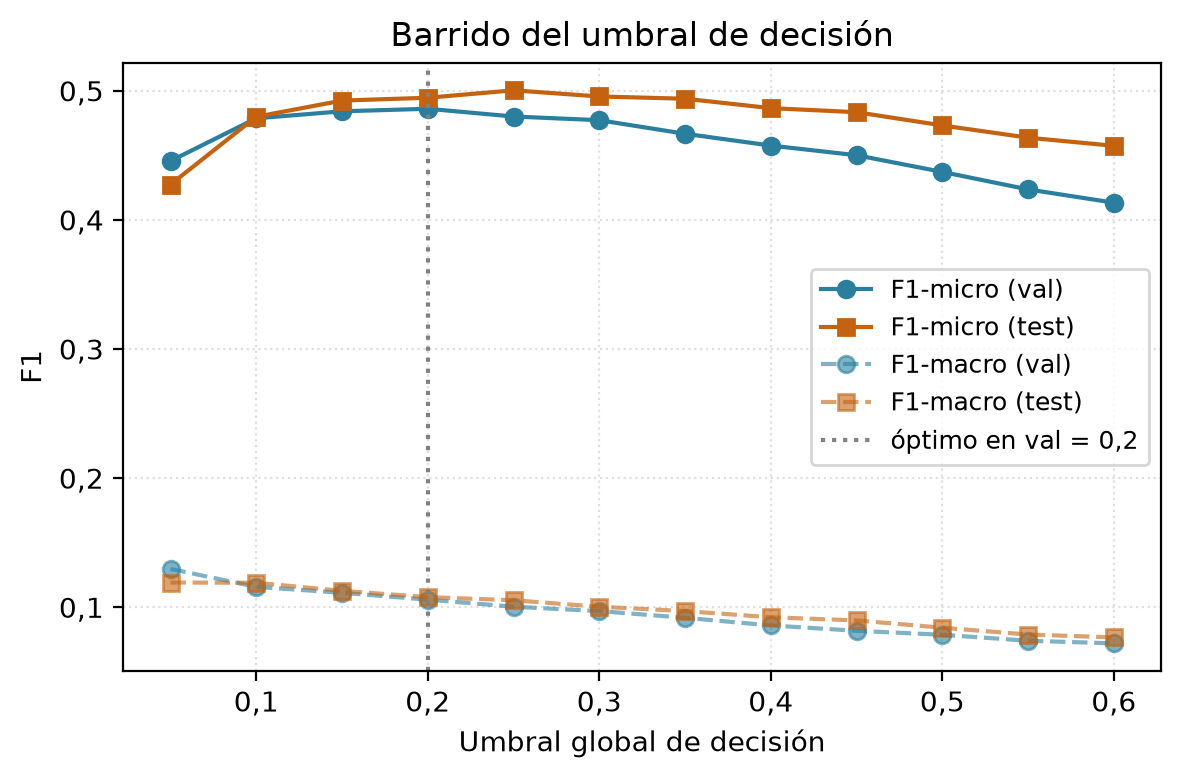
\includegraphics[width=0.72\textwidth]{figs/tfg_threshold}
\caption[Barrido del umbral global de decisión sobre validación y prueba]{Barrido del umbral global de decisión sobre validación y prueba. El F1-micro de validación se maximiza en 0,2 (umbral elegido); en prueba el máximo está en 0,25, a 0,6~pp del valor en 0,2, de modo que el umbral elegido sobre validación transfiere con una pérdida pequeña, aunque las curvas de precisión y \emph{recall} de ambas particiones difieren unos 4~pp en cada eje. El F1-macro decrece de forma monótona al subir el umbral.}
\label{fig:threshold}
\end{figure}

El mismo barrido, representado como curva precisión-\emph{recall} (Figura~\ref{fig:pr}), aporta dos lecturas que el barrido de F1 no deja ver. La primera es que la curva es prácticamente lineal en todo el rango útil: no hay codo ni punto de inflexión, de modo que cada punto de \emph{recall} ganado cuesta aproximadamente un punto de precisión y la elección del umbral es una decisión de política de uso, no un óptimo que la geometría de la curva imponga. El umbral 0,2 es simplemente el que maximiza el F1-micro, que pondera ambas por igual; para un sistema de ayuda a la codificación, donde el profesional revisa la propuesta y descartar un código erróneo cuesta menos que echar en falta uno correcto, un punto algo más orientado al \emph{recall} sería igualmente defendible. Se mantiene el óptimo de F1 por ser el criterio declarado de antemano y no ajustado a posteriori. La segunda lectura es que las curvas de validación y prueba se solapan casi por completo, lo que confirma que el umbral elegido sobre validación transfiere al conjunto de prueba y que la diferencia entre ambos conjuntos es de nivel, no de forma.

\begin{figure}[ht]
\centering
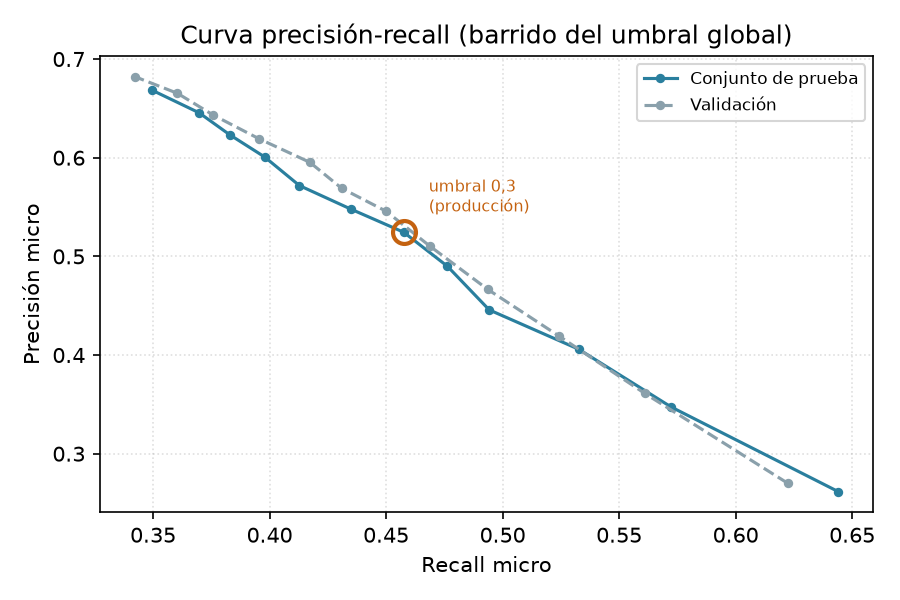
\includegraphics[width=0.72\textwidth]{figs/tfg_pr_curve}
\caption[Curva precisión-\emph{recall} del clasificador sobre validación y prueba, obtenida al barrer el umbral global de decisión]{Curva precisión-\emph{recall} del clasificador sobre validación y prueba, obtenida al barrer el umbral global de decisión. Se resalta el punto de operación de producción (umbral 0,2).}
\label{fig:pr}
\end{figure}

\paragraph{Modelos alternativos y granularidad de código (pasos 19--20).}
El modelo Longformer-BSC (\texttt{longformer-base-4096}, evaluado con una longitud de secuencia de 2.048 tokens) fue probado como alternativa para eliminar la truncación, que afecta a más de la mitad de los documentos (los que superan los 512 tokens). Pese a un recall superior (+5,8\,pp), el F1-micro cayó 1,4\,pp respecto a RigoBERTa-Clinical y el tiempo de entrenamiento aumentó 6,3× (70\,s/época frente a 11\,s). Una explicación posible, no contrastada, es que los diagnósticos clave se concentren en los primeros 512 tokens del informe y que el contexto adicional aporte más ruido que señal. RigoBERTa-Clinical con 512 tokens resultó la mejor opción de las ensayadas.

El paso al nivel de \emph{código completo} (1.767 clases, frente a 809 bloques de tres caracteres) conllevó una caída de 10\,pp en F1-micro: con 500 documentos de entrenamiento, la ratio datos/clase cae de $\sim$0,62 a $\sim$0,28. La degradación fue especialmente severa en F1-macro (0,118 → 0,050, $-$58\,\%), ya que códigos que aparecían 3 veces en train a nivel de bloque pasan a tener 1 aparición al subdividirse por subtipo. La elección de código completo para producción es correcta (el sistema clínico lo requiere), pero expone que el camino para recuperar esos 10\,pp pasa por aumentar los datos de entrenamiento, no por simplificar los objetivos.

\paragraph{Pre-entrenamiento débil (pasos 21--23).}
La escasez de datos para 1.767 clases motivó un pre-entrenamiento supervisado previo al \emph{fine-tuning} sobre CodiEsp. El mecanismo utiliza el catálogo CIE-10-ES como fuente de datos débilmente supervisados: para cada uno de los 1.767 códigos del vocabulario objetivo se extrae su descripción oficial (incluyendo variantes separadas por \texttt{|}) y se construye un par (descripción → código) que se usa como muestra de entrenamiento. De este modo el \emph{encoder} aprende a reconocer las \emph{keywords} clínicas de cada diagnóstico (terminología, siglas y variantes oficiales) antes de exponerse a las notas reales. En una ejecución, el pre-entrenamiento sobre las $\sim$3.200 variantes resultantes aportó +10,4\,pp de F1-micro (0,327 → 0,431). Añadir los 10.072 \emph{snippets} clínicos del task\_X de CodiEsp (fragmentos de texto real del médico anotados con su código) sumó 3,9\,pp adicionales (F1-micro=0,470) y una mejora del 51\,\% en F1-macro, porque esos \emph{snippets} enseñan la jerga real (\texttt{IAM}, \texttt{SCA}, \emph{dolor centrotorácico irradiado}) que el diccionario oficial no recoge. Un experimento de ablación con muestras negativas en el pre-entrenamiento resultó contraproducente; una explicación posible, no contrastada, es que el modelo aprenda a inhibir activaciones justo cuando necesita maximizar el reconocimiento de terminología.

\paragraph{Salvedad metodológica.} Los fragmentos del task\_X empleados en el pre-entrenamiento proceden de las particiones de entrenamiento \emph{y de validación} de CodiEsp, por lo que el modelo ha visto terminología anotada del conjunto sobre el que después se mide el F1-micro de validación. Es una contaminación parcial que conviene declarar: las cifras de validación deben leerse como una cota optimista. Su alcance está acotado por el propio conjunto de prueba, que no interviene en ninguna fase del entrenamiento: el F1-micro de prueba (0,4887) queda a solo 0,006 del de validación (0,4945), lo que indica que la ventaja obtenida es pequeña. Por este motivo, todas las cifras que se reportan como resultado final del trabajo se miden sobre el conjunto de prueba.

\paragraph{Experimentos con la función de pérdida (pasos 24 y 26).}
La Asymmetric Loss (ASL), que reduce o elimina la contribución de los negativos fáciles al gradiente, fue evaluada con $\gamma^- \in \{2, 4\}$. Con $\gamma^-=4$ el modelo colapsó al modo \emph{predecir todo} (F1-micro\,=\,0,375 frente a 0,470 de referencia). Con $\gamma^-=2$ el resultado fue prácticamente equivalente a BCE+pos\_weight ($-$1\,pp), sin beneficio neto. Subir el cap de pos\_weight de 10 a 30 no mejoró el resultado en las dos ejecuciones realizadas. La conclusión fue que el cuello de botella no es la ponderación de la función de pérdida sino la escasez de datos: con 999 códigos del vocabulario (el 56,5\,\%) vistos una sola vez y otros 568 con entre dos y cinco apariciones, es improbable que una ponderación compense la falta de ejemplos.

\paragraph{Técnicas de entrenamiento avanzadas y resultado final (pasos 28--32).}
Los últimos pasos introdujeron cuatro mejoras ortogonales que se acumularon en la configuración de producción:

\begin{itemize}
 \item \textbf{ReduceLROnPlateau} (paso 28b, +0,5\,pp): el \emph{schedule} coseno reducía el LR al 9\,\% del máximo en la época 60, cuando el modelo aún mejoraba. ReduceLROnPlateau mantiene el LR alto mientras hay mejora real y solo lo reduce cuando el F1 se estanca, permitiendo al modelo alcanzar su óptimo en la época 102.

 \item \textbf{Label smoothing one-sided} ($\varepsilon$=0,1, paso 29a, +0,68\,pp sobre 28b): suaviza los targets positivos de 1,0 a 0,9 pero mantiene los negativos en 0. El smoothing simétrico (0 → 0,05) colapsó el modelo al interaccionar con pos\_weight: el gradiente espurio de los negativos suavizados superó 13× al gradiente real de los positivos. La variante one-sided elimina esa interacción y reduce el sobreajuste de confianza en épocas tardías.

 \item \textbf{Descongelado progresivo} (paso 30b, unfreeze\_every=30, +0,23\,pp): a partir de la época 30 se descongelan 4 capas del \emph{encoder} cada 30 épocas con LR reducido ($10^{-5}$). Como hipótesis, no contrastada con una ablación por capas, las capas superiores son las más próximas a la tarea clínica y las que más necesitan adaptarse, mientras que las de bajo nivel (sintaxis, morfología) requerirían menos adaptación al dominio médico.

 \item \textbf{Regularizador de consistencia jerárquica} ($\lambda$=0,5, paso 32b, +0,46\,pp): CIE-10 tiene una estructura de árbol explícita (el código \texttt{J18.0} implica \texttt{J18}) que el clasificador plano ignora. Se añade el término $\ell_\text{hier} = \text{ReLU}(\text{logit}_\text{hijo} - \text{logit}_\text{padre})$ a la pérdida BCE con factor $\lambda=0{,}5$. La penalización es asimétrica: solo actúa cuando el hijo tiene logit superior al padre, sin interferir cuando el modelo ya es consistente. Con $\lambda=0{,}5$ se obtiene la mejor F1-micro del proceso; con $\lambda=0{,}1$ el mejor F1-macro por clase (+1,44\,pp respecto a la referencia), preferible cuando el objetivo es detección de códigos raros.
\end{itemize}

La Tabla~\ref{tab:progreso_pasos} recoge la evolución acumulada desde el clasificador plano sobre códigos completos hasta la configuración final, y la Figura~\ref{fig:waterfall} muestra la contribución de cada técnica al F1-micro resultante.

\begin{table}[h]
\centering
\small
\caption{Progreso acumulado del clasificador (F1 en validación CodiEsp, umbral global 0,3). Elaborada a partir de \texttt{model/\allowbreak{}training\_runs.csv} (ejecuciones de \texttt{make ai-train-gpu}) y del Anexo~\ref{cap:AnexoF}.}
\label{tab:progreso_pasos}
\begin{tabular}{P{1.0cm}P{7.0cm}rr}
\hline
\textbf{Paso} & \textbf{Técnica incorporada} & \textbf{F1-micro} & \textbf{F1-macro} \\
\hline
20 & Código completo sin preentrenamiento & 0,327 & 0,050 \\
21 & + Preentrenamiento sobre CIE-10 (3k descripciones) & 0,431 & 0,092 \\
23 & + Snippets clínicos task\_X (10k) & 0,470 & 0,139 \\
28b & + ReduceLROnPlateau & 0,475 & 0,116 \\
30b & + \emph{Label smoothing} + descongelado progresivo & 0,484 & 0,116 \\
\textbf{32b} & \textbf{+ Consistencia jerárquica ($\lambda$=0,5)} & \textbf{0,4888}$^\dagger$ & \textbf{0,120}$^\dagger$ \\
\hline
\end{tabular}
\smallskip\par\footnotesize $^\dagger$ Con umbral global de 0,3. Las cifras con umbrales por clase solo se conservan para la ejecución evaluada en profundidad (paso~36), y se recogen allí: aquí se omiten para no atribuir a 32b un dato que no se registró.
\end{table}

\begin{figure}[ht]
\centering
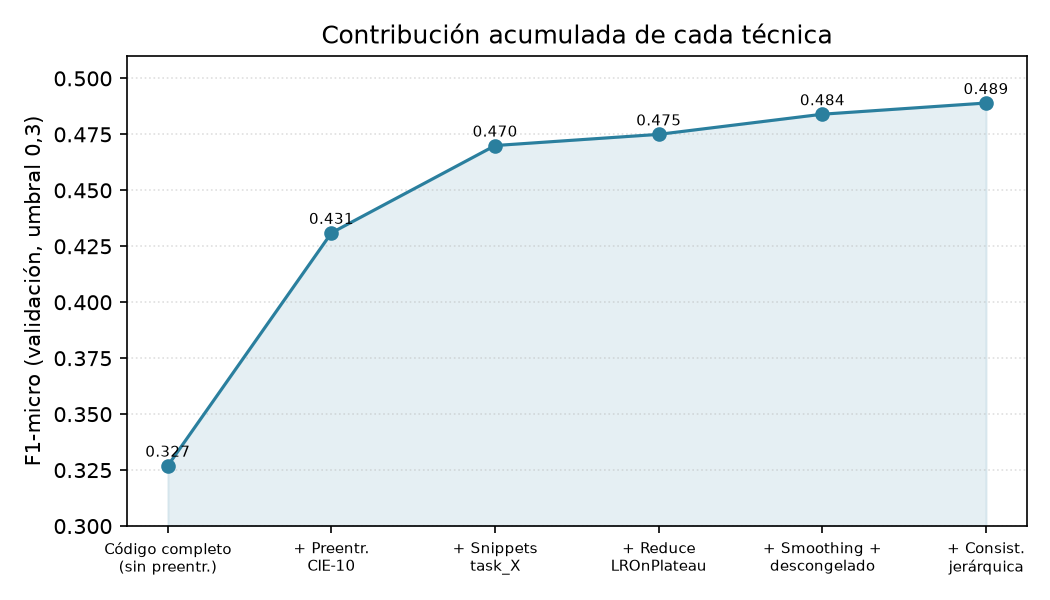
\includegraphics[width=0.78\textwidth]{figs/tfg_waterfall}
\caption{Contribución acumulada de cada técnica al F1-micro de validación (umbral 0,3), desde el clasificador plano inicial sobre códigos completos hasta la configuración final.}
\label{fig:waterfall}
\end{figure}

\subsubsection{Aumentación de datos mediante retrotraducción}
\label{sec:backtranslation}

El análisis de los experimentos anteriores reveló que la limitación principal no es la arquitectura ni la función de pérdida, sino la escasez de datos. El corpus de entrenamiento de CodiEsp contiene 500 documentos con una media de 11,28 etiquetas por nota, cubriendo los 1.767 códigos presentes en el corpus. La distribución de frecuencias es muy sesgada: el 56,5\,\% de los códigos aparece exactamente una vez y el 88,7\,\% no supera las cinco apariciones. Ninguna técnica de regularización puede compensar la escasez de señal de entrenamiento para las clases más raras.

La solución natural es generar datos sintéticos adicionales sin necesidad de anotación manual. La técnica empleada es la \textbf{retrotraducción} (\emph{back-translation})~\cite{sennrich2016improving}: cada nota clínica se traduce del español a un idioma pivote (inglés) y el resultado se vuelve a traducir al español. El texto final es semánticamente equivalente al original pero con diferente elección léxica y estructura sintáctica, actuando como una paráfrasis automática. Las etiquetas CIE-10 permanecen inalteradas porque la semántica clínica se conserva a través del pivote.

\paragraph{Generación y calidad del corpus aumentado.}
Con pivot EN se generaron 500 variantes retrotraducidas de las 500 notas originales, duplicando el corpus a 1000 documentos. La calidad de la traducción fue alta: el 99,2\,\% de las notas presentaron variación léxica efectiva, con un incremento medio de $+4{,}4$ palabras por nota (detalles en el Anexo~\ref{cap:AnexoL}). Para los 999 códigos que aparecían una sola vez, duplicar el número de ejemplos supone una mejora relativa del 100\,\% en la señal de entrenamiento. Las mejoras esperadas son:

\begin{itemize}
 \item \textbf{Códigos raros} (56,5\,\% del catálogo con una sola aparición): pasan a tener dos formulaciones distintas del mismo concepto, permitiendo al modelo aprender la invarianza semántica de cada código.
 \item \textbf{Robustez léxica}: el modelo deja de depender de formulaciones concretas del corpus original, ya que aprende la misma etiqueta asociada a expresiones diferentes.
 \item \textbf{F1-macro}: la métrica más sensible a las clases raras es la que más debería beneficiarse.
\end{itemize}

\paragraph{Implementación.}
Se diseñó el script \texttt{ai\_engine/augment.py} con dos \emph{backends} intercambiables: NLLB-200~\cite{costa-jussa2022nllb200} (modelo local de código abierto de Meta, sin coste externo) y Azure Translator (servicio en la nube con nivel gratuito de 2M caracteres/mes). El script incluye checkpoint incremental para reanudar traducciones interrumpidas. La integración con el flujo de entrenamiento se realiza mediante el target \texttt{make ai-augment} del \texttt{Makefile} y el parámetro \texttt{--train\_file} de \texttt{train.py}.

Se aplicaron tres pivotes independientes (EN, DE, FR), lo que cuadruplica el corpus de entrenamiento hasta 2.000 documentos. Las variantes se combinan mediante \texttt{ai\_engine/combine\_augmented.py} en un único CSV de entrenamiento. El proceso de configuración, los límites del servicio gratuito, las estadísticas de calidad por pivote y los comandos de uso se documentan en el Anexo~\ref{cap:AnexoL}.

\paragraph{Resultado del entrenamiento con datos aumentados.}
El entrenamiento con el corpus 4× se detuvo por \emph{early stop} en la época~51, antes de agotar el margen de épocas previsto. El resultado fue un F1-micro de \textbf{0,4668}, inferior al 0,4888 de referencia ($-0{,}022$). La causa más probable, que no se aisló con un experimento de control, es un desajuste en el \emph{schedule} de entrenamiento: con 2.000 documentos el número de pasos por época pasa de 63 a 250 (4×), pero el parámetro \texttt{UNFREEZE\_EVERY=30} no fue reescalado. Esto provoca que el primer descongelado de capas del \emph{encoder} ocurra tras 7500 pasos (frente a los 1890 del experimento de referencia), y es posible que el modelo converja en el régimen de \emph{freeze} total antes de que la señal de las capas superiores pueda aprovecharse, lo que explicaría el \emph{early~stop} en la época 51.

La hipótesis de trabajo es que al escalar el corpus conviene reescalar los hitos de unfreezing por la inversa del factor de datos: $\texttt{UNFREEZE\_EVERY} = \lceil 30 / 4 \rceil = 8$ para mantener el mismo número de pasos entre descongelados.

Durante el mismo experimento se observó además que el pre-entrenamiento estaba sobreajustado: la pérdida de \emph{pretrain} cae de 0,76 en el primer paso a 0,0038 al final de la época~1 y llega a 0,0008 en la época~6, esencialmente cero. Con la pérdida de \emph{pretrain} prácticamente nulo desde la época~6, las épocas 7--10 aparentaban ser prescindibles: no aportan señal nueva a la función de pérdida. El experimento de corrección (\emph{paso~33b}) aplica dos ajustes simultáneos: \texttt{UNFREEZE\_EVERY=8} y \texttt{PRETRAIN\_EPOCHS=3}, con la hipótesis de ahorrar $\sim$28~minutos de pre-entrenamiento y partir de una inicialización menos sobreajustada.

\paragraph{Pasos 33 a 35: qué se intentó y qué se aprendió.}
Tras fijar la configuración de referencia (32b, F1-micro~0,4888) se ensayaron tres vías para superarla: entrenar sobre el corpus aumentado por retrotraducción, aumentar el \emph{batch} efectivo a 64 mediante acumulación de gradiente, y acortar el preentrenamiento a 3 épocas dando a cambio más margen de entrenamiento. Ninguna la superó, y la Tabla~\ref{tab:paso35} recoge las cuatro variantes del paso~35 frente a la referencia. El desarrollo completo de cada ejecución, con sus cifras por época, está en el Anexo~\ref{cap:AnexoF}.

Las tres dejan una lección transferible, que es lo que justifica haberlas intentado:

\begin{itemize}
 \item \textbf{Entrenar con texto retraducido y validar con texto original puede abrir una brecha de distribución.} Una explicación plausible, no contrastada con un experimento de control, es que el modelo aprenda construcciones sintácticas características de la retraducción que el conjunto de validación, en español original, penaliza. Los datos sintéticos añaden variedad léxica, pero en estos experimentos no mejoraron el resultado.
 \item \textbf{Los hiperparámetros de calendario parecen depender del tamaño del corpus.} Con 500 documentos y \emph{batch}~8 hay 63 mini-lotes por época, de modo que acumular 8 deja solo 7 actualizaciones del optimizador por época frente a las 15 de la referencia. Con esa cadencia el \emph{scheduler} apenas recibe señal y el descongelado progresivo opera con gradientes menos informativos. \texttt{GRAD\_ACCUM}, \texttt{UNFREEZE\_EVERY} y \texttt{PATIENCE} fijan una cadencia por época y hay que recalibrarlos cada vez que cambia el número de muestras.
 \item \textbf{Que la pérdida de preentrenamiento llegue a cero no significa que esas épocas sobren.} Recortarlas de 10 a 3 costó 0,025 de F1-micro con todo lo demás idéntico, y restaurarlas recuperó el mismo valor de la referencia (con una sola ejecución por variante). La saturación aparente de la pérdida podría no ser sobreajuste evitable, sino convergencia gradual de las representaciones.
\end{itemize}

\begin{table}[h]
\centering
\small
\caption{Resumen del paso~35: comparativa de variantes frente a la ejecución de referencia 32b (F1 con umbral global 0,3). Cada F1 y su mejor época salen del historial por época de la ejecución (\texttt{model/\allowbreak{}training\_history\_*.json}, Anexo~\ref{cap:AnexoF}); \texttt{training\_runs.csv} registra 0,4651 para 35a y 0,4785 para 35d al reevaluar el \emph{checkpoint} guardado.}
\label{tab:paso35}
\begin{tabular}{llrrr}
\hline
\textbf{Ejec.} & \textbf{Corpus} & \textbf{F1-micro} & \textbf{F1-macro} & \textbf{Mejor época} \\
\hline
\textbf{32b (referencia)} & \textbf{500 docs originales} & \textbf{0,4888} & \textbf{0,1196} & \textbf{135} \\
35a & 500 docs, pretrain=3 & 0,4643 & 0,0990 & n/d \\
35b & 2000 docs (BT), pretrain=3 & 0,4569 & n/d & n/d \\
35c & 500 docs, pretrain=10 & 0,4888 & 0,1110 & 124 \\
35d & 2000 docs (BT), pretrain=10 & 0,4766 & 0,1140 & 29 \\
\hline
\end{tabular}
\end{table}

El artefacto de referencia de la selección de hiperparámetros es la ejecución del \textbf{paso~36} (el modelo que se sirvió hasta su sustitución por \texttt{zlpr-map}, descrita en el Anexo~\ref{cap:AnexoH}; las cifras y el umbral de 0,3 de este párrafo son los del paso~36, no los del modelo desplegado ahora), que reproduce la configuración de 32b sin modificar ningún hiperparámetro. Fue en su momento la mejor ejecución por F1-micro de validación, si bien su ventaja sobre 32b ($+0{,}006$) queda dentro del intervalo de variabilidad estocástica ($\pm 0{,}01$) discutido más adelante: se elige por ser el artefacto entrenado más reciente con esa configuración, no por una superioridad estadísticamente significativa. Sobre validación obtiene F1-micro~0,4945 y F1-macro~0,119 con umbral global de 0,3, el óptimo del barrido de umbrales, y sobre el conjunto de prueba F1-micro~0,4887 y F1-macro~0,109. Los umbrales por clase optimizados sobre validación elevan el F1-micro de validación a 0,551, pero \emph{no generalizan}: sobre el conjunto de prueba caen a 0,468, por debajo del umbral global, por lo que la configuración de producción emplea el umbral global. Corpus: 500 documentos originales, \texttt{PRETRAIN\_EPOCHS=10}. Esta ejecución, \texttt{classifier\_20260530T030233Z\_f1=0.4945.pt}, está publicada en HuggingFace\footnote{\url{https://huggingface.co/dmartingarcia/cie10-rigoberta-classifier}}; los detalles de evaluación se recogen en el Anexo~\ref{cap:AnexoH}. El entrenamiento no se detiene en este punto: la \textbf{política de despliegue} consiste en sustituir el artefacto de producción por el mejor modelo disponible tras confirmar sus cifras en el conjunto de prueba, no solo en validación (una F1-micro de validación más alta no basta si no se sostiene en prueba, como documenta la sección~\ref{sec:anexoH-candidatos}), sin necesidad de modificar código, únicamente actualizando \texttt{ai\_engine/model/config.json}. El Anexo~\ref{cap:AnexoF} recoge la tabla completa de ejecuciones con sus valores de F1-micro y MAP, y debe consultarse para conocer cuál es la configuración vigente en cualquier instante posterior al cierre de este documento; las vías de mejora restantes se recogen en la sección de trabajos futuros de las conclusiones.

\paragraph{La pérdida de ordenación del modelo servido.} El modelo que sirve el sistema, \texttt{zlpr-map} (ejecución \texttt{20260921T091919Z}), parte de la configuración del paso~36 y modifica dos elementos, ambos solo en el entrenamiento y sin coste de inferencia. El primero es un término de ordenación ZLPR~\cite{su2022zlpr}, con peso 0,1, que se suma a la entropía cruzada: penaliza que un código incorrecto de un informe quede por encima de uno correcto del mismo informe, que es lo que mide el MAP, sin exigir un valor absoluto de probabilidad. El segundo es elegir el \emph{checkpoint} por MAP de validación en lugar de por F1-micro, porque bajo entropía cruzada el MAP resultaba poco informativo y con el nuevo término vuelve a serlo. Con cuatro semillas, el MAP medio de prueba pasa de 0,4359 (cinco réplicas de control) a 0,4466, una diferencia de $+1{,}08$~pp (prueba $t$ de Welch, $p=0{,}045$) que es evidencia moderada y no concluyente. El modelo desplegado, de ese grupo, obtiene MAP 0,454 y F1-micro 0,495 frente a 0,437 y 0,488 del paso~36 (Anexo~\ref{cap:AnexoF}, sección~\ref{sec:anexoF-alineacion}, y Tabla~\ref{tab:candidatos} del Anexo~\ref{cap:AnexoH}).

La Tabla~\ref{tab:codiesp-comparativa} sitúa el modelo en el contexto del \emph{benchmark} CodiEsp-D 2020, la tarea compartida de referencia para codificación automática de diagnósticos clínicos en español~\cite{miranda2020}. El MAP de este trabajo se calcula sobre el mismo conjunto de prueba que emplearon los equipos participantes, por lo que la comparación es homogénea. El sistema se compara en sus dos configuraciones ejecutables. En la configuración por defecto, con el clasificador solo, obtiene un MAP de 0,454, que lo sitúa en el penúltimo lugar de la tabla, por delante únicamente de IMS. En \textbf{modo fusionado}, combinando el clasificador con el diccionario en un único \emph{ranking}, alcanza \textbf{0,554 y pasa a la segunda posición}, por delante de todos los demás sistemas de la tabla, incluidos los diccionarios construidos a mano y los basados en \emph{transformers}, y solo por detrás de IXA-AAA (XGBoost con BERT multilingüe). La diferencia entre ambas filas, diez puntos de MAP, es el resultado más relevante de este trabajo: no procede de un modelo mejor sino, probablemente, de combinar dos fuentes de evidencia que fallan en sitios distintos. Una salvedad: $\beta$ y el umbral se eligen sobre validación, pero el diccionario incorpora anotaciones del conjunto de validación (fuente \emph{clinical}), de modo que el ajuste en validación es optimista; la cifra de prueba no está contaminada, porque el diccionario nunca usa ese conjunto. Restringido al vocabulario de 1.767 códigos que el modelo puede predecir, el MAP de la configuración por defecto asciende a 0,555, pero esa cifra no es comparable con el resto de sistemas, que podían proponer cualquier código del catálogo. Las cifras de prueba del modelo servido citadas en este capítulo proceden del guion de evaluación en precisión completa (\texttt{eval\_test.py}), salvo la del modo fusionado (\texttt{motores\_eval.py}); los experimentos del Anexo~\ref{cap:AnexoF} emplean una pasada en precisión reducida que permite comparar muchos modelos entre sí en una sola ejecución y que sitúa este mismo modelo en 0{,}4535. La diferencia, de 0{,}04~pp, no afecta a ninguna conclusión, pero conviene no mezclar ambas procedencias al citar cifras.

Conviene cuantificar esa restricción antes de leer las cifras de \emph{recall}. De los 2.842 pares documento-código del \emph{gold} de prueba, 497 (el 17,5\,\%) corresponden a códigos ausentes del vocabulario de entrenamiento: ninguna arquitectura con este espacio de salida puede acertarlos. El \textbf{techo de recall} queda por tanto en 0,825. Hay que precisar sobre qué \emph{gold} se calculan la precisión, el \emph{recall} y el F1 de este trabajo: \texttt{eval\_test.py} los mide sobre los 2.345 pares alcanzables, de modo que el \emph{recall} de 0,459 es el del \emph{gold} alcanzable. Sobre el \emph{gold} completo de 2.842 pares, que es el que usan los equipos del \emph{benchmark}, los mismos 1.077 aciertos dan un \emph{recall} de 0,379 y un F1-micro de 0,444 (precisión 0,536). El MAP estricto sí penaliza los códigos inalcanzables y no se ve afectado. La diferencia entre ambas lecturas es la restricción estructural descrita en el análisis exploratorio (sección~\ref{sec:analisis_datos}), y es la razón por la que la vía de mejora pasa por ampliar el corpus anotado y no por cambiar de arquitectura.

\paragraph{De qué depende realmente el rendimiento.}
El análisis exploratorio mostró que la distribución de códigos sigue una ley de potencia; lo que no mostraba es cuánto cuesta eso en rendimiento. Agrupando los 1.767 códigos del vocabulario por su número de apariciones en el corpus de entrenamiento y midiendo cada grupo por separado sobre el conjunto de prueba se obtiene la relación de la Figura~\ref{fig:freq}, que es monótona y muy pronunciada: los 999 códigos vistos una sola vez alcanzan un F1-micro de 0,122, los vistos entre dos y cinco veces 0,328, y los 33 códigos con más de veinte apariciones llegan a 0,671. Esos 33 códigos, el 1,9\,\% del vocabulario, concentran 671 de los 2.345 pares alcanzables del \emph{gold} de prueba.

Una lectura posible es que el rendimiento por código depende sobre todo de cuántas veces lo ha visto el modelo. Es la misma tendencia que sugería la brecha entre F1-micro y F1-macro, medida ahora directamente: el F1-micro global de 0,495 es el promedio ponderado de un modelo que rinde razonablemente sobre el puñado de códigos frecuentes y que apenas reconoce la cola larga. Los cambios de arquitectura y de hiperparámetros de los pasos 24 a 35 no movieron el F1 más allá de la variabilidad entre ejecuciones (en torno a $\pm 0{,}01$), mientras que lo que sí elevó el MAP sin datos nuevos fue la pérdida de ordenación (aproximadamente $+1$~pp) y la fusión con el diccionario (unos 10~pp). Con los datos disponibles, ampliar el corpus anotado parece la vía con más recorrido para la cola larga, aunque no necesariamente la única; y la relación entre frecuencia y F1 puede estar mezclada con la dificultad propia de cada código, algo que esta medición no permite separar.

\begin{figure}[ht]
\centering
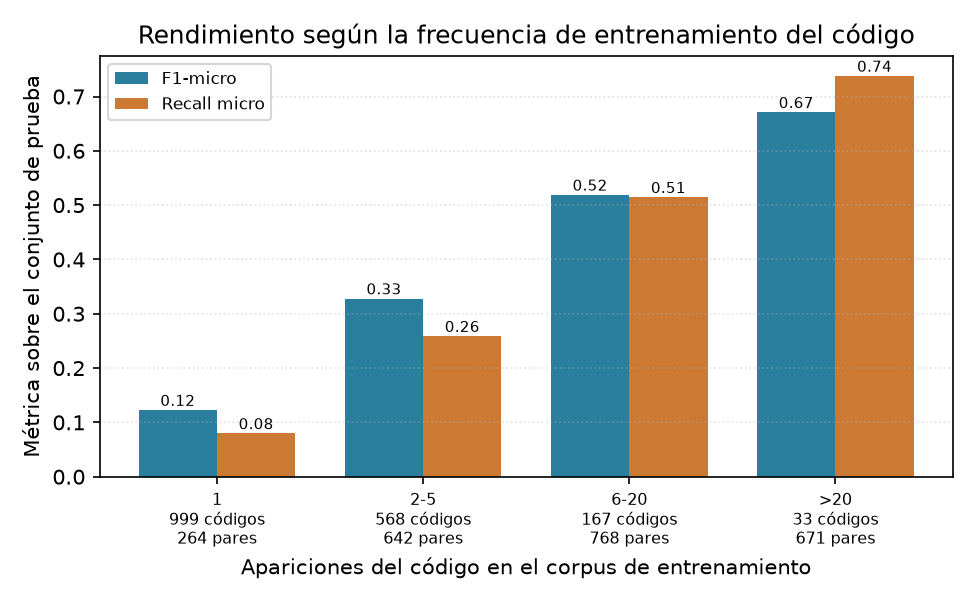
\includegraphics[width=0.75\textwidth]{figs/tfg_freq}
\caption{F1-micro y \emph{recall} sobre el conjunto de prueba según el número de apariciones del código en el corpus de entrenamiento (umbral 0,2, modelo desplegado). Bajo cada grupo se indica cuántos códigos lo forman y cuántos pares del \emph{gold} aportan.}
\label{fig:freq}
\end{figure}

La Figura~\ref{fig:benchmark} representa gráficamente esa clasificación y la Figura~\ref{fig:chapters} desglosa el rendimiento del modelo por capítulo CIE-10. La cifra reportada corresponde al modelo desplegado, que es el sistema que este trabajo presenta; la comparación de los candidatos que llevó a elegirlo está en la sección~\ref{sec:anexoH-candidatos}. Una observación preliminar recogida en el Anexo~\ref{cap:AnexoF} (sección~\ref{sec:anexoF-map}) apunta a que promediar las salidas de varias ejecuciones reduce la varianza y mejora el MAP; no se ha diseñado ni evaluado un sistema de combinación como tal, por lo que no se reporta como resultado y queda planteado como línea futura.

\begin{table}[h]
\centering
\small
\caption{Comparación con los sistemas del \emph{benchmark} CodiEsp-D (CLEF 2020)~\protect\cite{miranda2020}. Todas las métricas se calculan sobre el conjunto de prueba. Los equipos externos entregan listas de códigos ordenados por confianza (sin umbral de decisión), lo que explica sus valores de F1 muy bajos con \emph{recall} alto; el F1 de este trabajo corresponde a una decisión binaria con umbral global de 0,2, medida sobre el \emph{gold} alcanzable (sobre el completo, el \emph{recall} es 0,379 y el F1 0,444), y no es directamente comparable con esa columna. La métrica homogénea es el MAP por documento. Las dos filas sombreadas son este trabajo. Generada con \texttt{make ai-eval-test} (fila del clasificador solo, \texttt{model/\allowbreak{}eval\_test.json}) y \texttt{make ai-motores} (fila fusionada, \texttt{model/\allowbreak{}comparativa\_motores.json}); las filas de los demás equipos se transcriben de la Tabla~7 de~\cite{miranda2020}.}
\label{tab:codiesp-comparativa}
\begin{tabular}{P{3.6cm}P{4.0cm}rrrr}
\hline
\textbf{Sistema} & \textbf{Enfoque} & \textbf{P} & \textbf{R} & \textbf{F1} & \textbf{MAP} \\
\hline
IXA-AAA & XGBoost + BERT Multilingüe & 0{,}004 & 0{,}858 & 0{,}009 & \textbf{0{,}593} \\
\rowcolor{gray!15}
\textbf{Modo fusionado} & Clasificador + diccionario en un solo \emph{ranking} & 0{,}642 & 0{,}582 & 0{,}610 & \textbf{0{,}554}$^{*}$ \\
IAM & Diccionario + coincidencia exacta/Levenshtein & 0{,}817 & 0{,}592 & \textbf{0{,}687} & 0{,}521 \\
FLE & Sistema clínico multilingüe propietario & 0{,}740 & 0{,}633 & 0{,}679 & 0{,}519 \\
The Mental Strokers & BETO \emph{fine-tuning} & 0{,}759 & 0{,}638 & 0{,}591 & 0{,}517 \\
LSI-UNED & Recuperación de información + expansión & 0{,}253 & 0{,}688 & 0{,}370 & 0{,}517 \\
Anuj & BERT + búsqueda léxica & 0{,}741 & 0{,}621 & 0{,}676 & 0{,}505 \\
MEDIA & Ensamble con BETO & 0{,}735 & 0{,}630 & 0{,}629 & 0{,}488 \\
ICB-UMA~\cite{lopezgarcia2020icb} & BERT-SciELO \emph{fine-tuning} & 0{,}004 & 0{,}897 & 0{,}009 & 0{,}482 \\
\rowcolor{gray!15}
\textbf{Este trabajo (clasificador solo)} & RigoBERTa-Clinical \emph{fine-tuning} & 0{,}536 & 0{,}459 & 0{,}495 & 0{,}454 \\
IMS & CNN + atención & 0{,}373 & 0{,}709 & 0{,}474 & 0{,}449 \\
\hline
\end{tabular}

\vspace{2mm}
{\footnotesize Nota: en la fuente, las filas de The Mental Strokers (F1 0,591), MEDIA (0,629) e IMS (0,474) no cumplen $F1=2PR/(P+R)$ con las P y R impresas (daría 0,693, 0,678 y 0,489); se transcriben tal cual, y la discrepancia podría deberse a que cada columna procede de una ejecución distinta del equipo, pero el artículo no lo aclara.

\vspace{1mm}
\footnotesize $^{*}$ El modo fusionado combina el clasificador y el diccionario en un único
\emph{ranking} y está implementado en el motor (\texttt{engine=fused}), pero la configuración que
el sistema sirve por defecto es la del clasificador solo. Su cifra procede de
\texttt{make ai-motores} (\texttt{ai\_engine/\allowbreak{}motores\_eval.py}), que reproduce la fusión tal como
la implementa el motor y deja el barrido de $\beta$ en \texttt{model/\allowbreak{}fusion\_sweep.json}: medido en
esa misma pasada, el clasificador solo obtiene 0,454, la misma cifra que da la evaluación en
precisión completa, de modo que la ganancia atribuible a la fusión es de 10,0 puntos en ambas
procedencias. Se muestran las dos configuraciones porque ambas son ejecutables.}
\end{table}

\begin{figure}[ht]
\centering
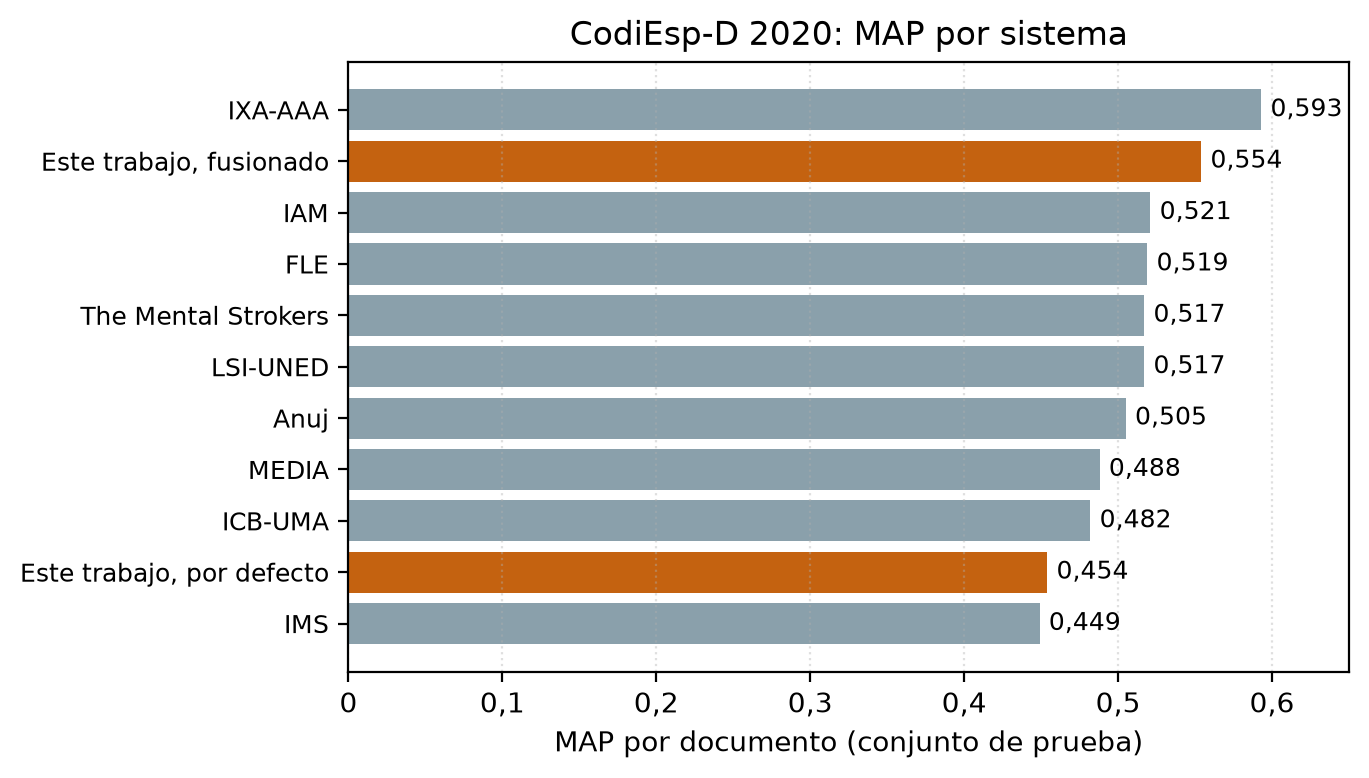
\includegraphics[width=0.8\textwidth]{figs/tfg_benchmark}
\caption[MAP por documento de los sistemas del \emph{benchmark} CodiEsp-D 2020 sobre el conjunto de prueba, con este trabajo resaltado]{MAP por documento de los sistemas del \emph{benchmark} CodiEsp-D 2020 sobre el conjunto de prueba, con este trabajo resaltado. Las primeras posiciones las ocupan \emph{ensembles} y diccionarios construidos manualmente.}
\label{fig:benchmark}
\end{figure}

\begin{figure}[ht]
\centering
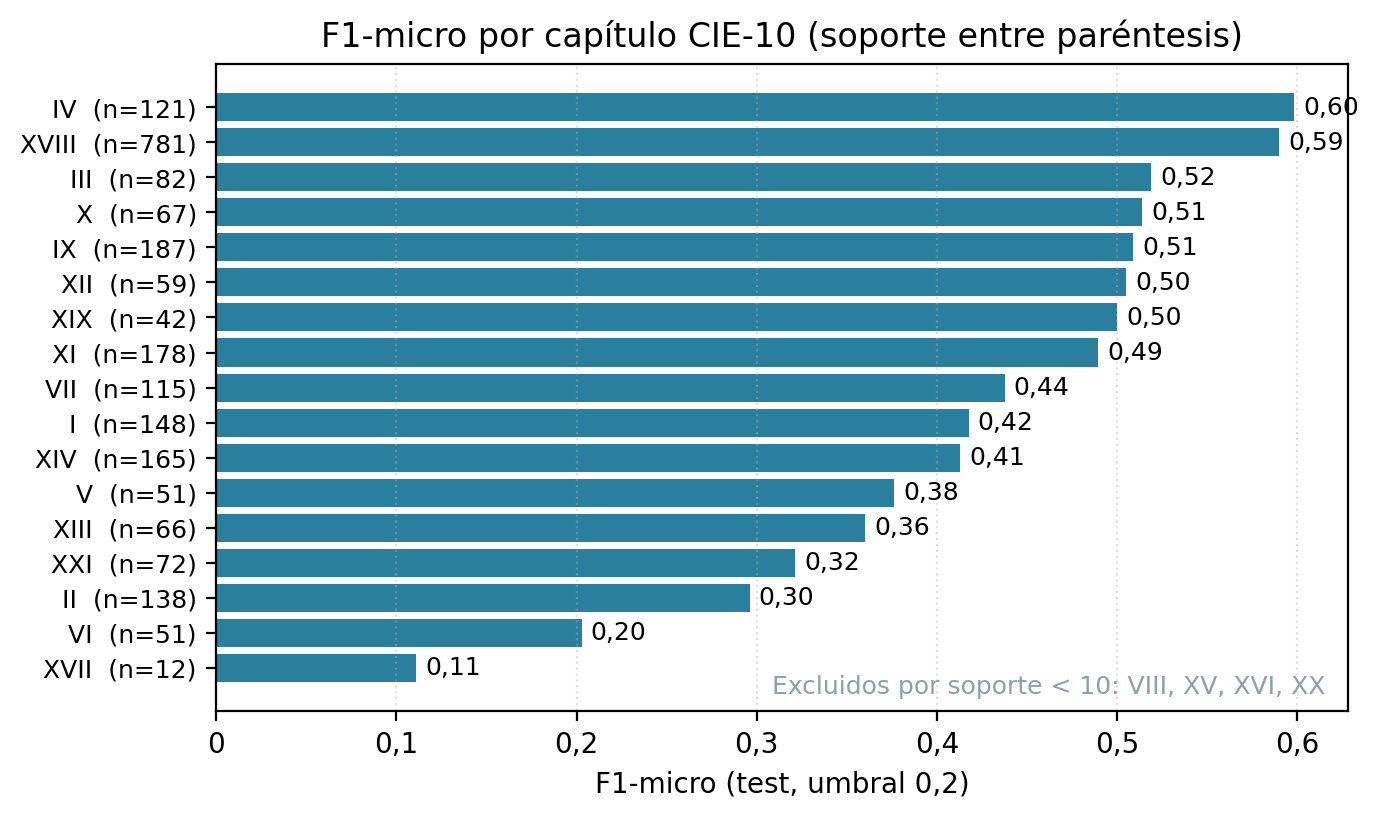
\includegraphics[width=0.75\textwidth]{figs/tfg_chapters}
\caption[F1-micro por capítulo CIE-10 sobre el conjunto de prueba (umbral 0,2, modelo desplegado), con el soporte de cada capítulo entre paréntesis]{F1-micro por capítulo CIE-10 sobre el conjunto de prueba (umbral 0,2, modelo desplegado), con el soporte de cada capítulo entre paréntesis. Se excluyen los capítulos con menos de diez pares en el \emph{gold} (VIII, XV, XVI y XX), donde el F1 carece de sentido estadístico. La equivalencia entre cada número romano y el capítulo de la CIE-10-ES se recoge en la Tabla~\ref{tab:capitulos-cie10} del Anexo~\ref{cap:AnexoG}.}
\label{fig:chapters}
\end{figure}

A nivel de capítulo la relación con la frecuencia de entrenamiento es solo moderada ($r=0{,}40$ sobre los diecisiete capítulos con soporte suficiente, una muestra pequeña, por lo que es una cifra orientativa), bastante más débil que la que se observa por código en la Figura~\ref{fig:freq}. Una razón probable es que un capítulo agrupa códigos muy heterogéneos, de modo que su F1 depende menos del volumen total de ejemplos que de cómo se reparten: dos capítulos con el mismo número de pares rinden de forma muy distinta según si esos pares se concentran en unos pocos códigos o se dispersan en muchos.

El capítulo~XVII (malformaciones congénitas) es el que peor rinde entre los capítulos con soporte suficiente, con F1-micro de 0,111 sobre 82 pares de entrenamiento. Con solo 12 pares en el \emph{gold} de prueba, esa cifra equivale a un acierto sobre pocas propuestas y es muy inestable; probablemente refleja códigos de malformaciones muy específicos y dispersos, con pocos ejemplos cada uno, más que una dificultad propia del capítulo. Como ilustración del mecanismo, y no como prueba, el capítulo~VI (enfermedades del sistema nervioso) permite aislarlo del volumen total: tiene exactamente el mismo soporte en prueba que el capítulo~V (51 pares) y una frecuencia de entrenamiento comparable (125 pares frente a 158), pero un F1 de 0,203 frente a 0,376, casi la mitad. La diferencia está en la concentración: los 125 pares del capítulo~VI se reparten entre \textbf{67 códigos distintos} (1,9 apariciones por código, y el más frecuente aparece solo ocho veces), mientras que los 158 del capítulo~V se concentran en \textbf{47 códigos} dominados por un puñado muy repetido, encabezado por los códigos de consumo de tabaco (\texttt{F17.210} aparece 28 veces) y la depresión no especificada (\texttt{F32.9}, 14 veces). Con un solo par de capítulos no se puede generalizar, pero el capítulo~VI se parece a la cola larga pura: neurología con muchos diagnósticos diferentes y casi ningún ejemplo por diagnóstico.

\subsubsection*{En qué se equivoca el modelo}

Las métricas agregadas dicen cuánto falla el clasificador, no en qué falla. Para saberlo se etiqueta cada error del conjunto de prueba según su distancia al código correcto: si comparte el bloque de tres caracteres con alguno de los anotados en ese documento, el error es de especificidad (el modelo entendió la patología y erró el grado de detalle); si comparte capítulo pero no bloque, erró dentro del área clínica correcta; si cae en otro capítulo, es un error de comprensión. El análisis se genera con \texttt{make ai-error-analysis} sobre el modelo desplegado (umbral 0,2) y queda en \texttt{model/error\_analysis.json}.

Lo primero que revela es que el modelo \textbf{subpredice}: propone 8,04 códigos por documento frente a los 11,37 anotados. No es un fallo de calibración menor, es la explicación directa de que el \emph{recall} quede por debajo de la precisión, y encaja con un umbral fijo aplicado a probabilidades que el desequilibrio de clases mantiene bajas.

\begin{table}[h]
\centering
\small
\caption{Errores del modelo sobre el conjunto de prueba, clasificados por distancia al código correcto (umbral 0,2, modelo desplegado). Generada con \texttt{make ai-error-analysis} (\texttt{model/\allowbreak{}error\_analysis.json}).}
\label{tab:analisis-error}
\begin{tabular}{lrrrr}
\hline
 & \textbf{Total} & \textbf{Mismo bloque} & \textbf{Mismo capítulo} & \textbf{Otro capítulo} \\
\hline
Falsos positivos & 933 & 209 (22,4\,\%) & 586 (62,8\,\%) & 138 (14,8\,\%) \\
Falsos negativos & 1.765 & 230 (13,0\,\%) & 847 (48,0\,\%) & 688 (39,0\,\%) \\
\hline
\end{tabular}
\end{table}

La lectura de la Tabla~\ref{tab:analisis-error} es favorable en un sentido y preocupante en otro. Cuando el modelo propone un código que no estaba anotado, el 85,2\,\% de las veces acierta al menos el capítulo, y algo más de una quinta parte de esos casos son códigos hermanos del correcto: fallos de grado de detalle, no de entendimiento. Un codificador que revise esa lista descarta el código pero conserva la pista. En cambio, el 39,0\,\% de los códigos que el modelo deja escapar pertenece a capítulos que no ha tocado en ese documento, de modo que el \emph{recall} no se arregla bajando el umbral: falta señal, no sensibilidad.

El desglose por código apunta a la misma causa en los dos sentidos. R52 («dolor, no especificado») encabeza los falsos positivos (39 casos) y aparece también entre los falsos negativos (20, empatado con R69, «enfermedad, no especificada»); completan el grupo N28.9 («trastorno del riñón y del uréter, no especificado», 22 falsos positivos) y R53.1 («astenia», 22). Son códigos residuales, los que el manual reserva para cuando el informe menciona el hallazgo pero no lo concreta. Asignarlos correctamente depende de lo que el documento \emph{no} dice, y un clasificador que puntúa cada etiqueta a partir de lo que sí aparece en el texto no tiene forma de representar esa ausencia. Es una limitación de la formulación del problema, no del entrenamiento, y por eso conviene declararla en lugar de atribuirla a falta de datos.

\paragraph{Nota sobre reproducibilidad y variabilidad entre ejecuciones.}
\begin{sloppypar}
El script de entrenamiento admite fijar la semilla aleatoria (\emph{random seed}) con \texttt{--seed}, pero no se utilizó en los experimentos. Esta decisión fue deliberada durante la fase exploratoria: fijar la semilla habría requerido activar \texttt{torch.use\_deterministic\_algorithms} y \texttt{CUBLAS\_WORKSPACE\_CONFIG}, lo que deshabilita kernels CUDA optimizados e incrementa el tiempo de entrenamiento de forma apreciable. En un proceso iterativo de decenas de ejecuciones (más de setenta registradas a fecha de cierre de este documento), ese sobrecoste habría sido prohibitivo.
\end{sloppypar}

La contrapartida es que los resultados no son exactamente reproducibles. Las fuentes de no-determinismo son tres: la inicialización aleatoria de la cabeza clasificadora, el orden de los mini-batches en cada época y las operaciones CUDA no deterministas (operaciones de reducción en paralelo, Flash Attention). En la práctica, la variabilidad observada entre ejecuciones con configuración idéntica es de $\pm 0{,}01$ en F1-micro, lo que no altera las conclusiones comparativas entre pasos pero sí impide replicar el valor exacto 0,4945 del paso~36. Los experimentos del 33 al 35 sirven para confirmar que esa configuración es robusta, no para superarla de forma reproducible.

Para un ciclo de reentrenamiento productivo con datos reales se recomienda fijar \texttt{--seed} y guardar la semilla en \texttt{config.json}, de modo que cada modelo desplegado sea auditable; el registro de ejecuciones ya dispone de una columna \texttt{seed} para anotarla.

\paragraph{Paso 36}
\begin{sloppypar}
Tras confirmar en los pasos 33--35 que ninguna modificación de hiperparámetros mejoraba de forma robusta la referencia 32b, se realizó una reejecución con la configuración exacta de 32b para explotar la variabilidad estocástica inherente al entrenamiento. El resultado fue F1-micro~\textbf{0,4945} en validación ($+0{,}006$ respecto a 32b) y F1-macro~0,119. La ejecución completó las 150~épocas en \textbf{27~minutos} ($\sim$11~s/época). La ganancia en F1-micro, dentro del intervalo de variabilidad estocástica $\pm 0{,}01$, se debe a una inicialización aleatoria más favorable. Sobre el conjunto de prueba el modelo obtiene F1-micro~0,4887 (umbral global 0,3) y un MAP por documento de \textbf{0,437} sobre el gold completo, la métrica oficial del \emph{benchmark}, lo que lo sitúa dentro del rango de los sistemas de CodiEsp 2020~\cite{miranda2020}, por detrás de los \emph{ensembles} y diccionarios de las primeras posiciones (véase Tabla~\ref{tab:codiesp-comparativa}). Este modelo, \texttt{classifier\_20260530T030233Z\_f1=0.4945.pt}, fue la ejecución de referencia durante la mayor parte del trabajo. La comparación final de candidatos sobre el conjunto de prueba (sección~\ref{sec:anexoH-candidatos}) lo desplazó en favor de la ejecución con pérdida de ordenación de la subsección~\ref{sec:anexoF-alineacion}, que lo supera en MAP, MAP fusionado y F1-micro a la vez; sus cifras se conservan aquí porque son las que sostienen la lectura de este paso.

El comando empleado para esta ejecución fue:
\begin{lstlisting}[language=bash,basicstyle=\small\ttfamily,showstringspaces=false]
FULL_CODES=1 MAX_LENGTH=512 FREEZE_LAYERS=20 LR=1e-4 DROPOUT=0.3 \
WEIGHT_DECAY=0.1 THRESHOLD=0.3 BATCH_SIZE=8 GRAD_ACCUM=4 \
EPOCHS=150 PATIENCE=20 LR_SCHEDULE=plateau LABEL_SMOOTHING=0.1 \
UNFREEZE_EVERY=30 UNFREEZE_LAYERS=4 UNFREEZE_LR_RATIO=0.1 \
LAMBDA_HIER=0.5 PRETRAIN_EPOCHS=10 \
PRETRAIN_TASKX="/data/codiesp_csvs/\
codiesp_X_source_train.csv \
 /data/codiesp_csvs/\
codiesp_X_source_validation.csv" \
make ai-train-gpu
\end{lstlisting}
\end{sloppypar}

\subsubsection{Aprendizaje continuo a partir de la retroalimentación de los usuarios}
\label{sec:continuous-learning}

Una limitación estructural del entrenamiento sobre CodiEsp es que los datos proceden de
un \emph{benchmark} con distribución fija. En un entorno clínico real, el modelo encontrará
patrones de redacción, abreviaturas y combinaciones de códigos que difieren del corpus de
entrenamiento. Para cerrar esta brecha, el sistema está diseñado para capturar señal de
retroalimentación de los propios codificadores y reutilizarla en ciclos de reentrenamiento
posteriores.

\paragraph{Datos capturados por el sistema.}
Cada sesión de análisis genera un registro inmutable de eventos en el \emph{event store}
del backend (véase la sección~\ref{sec:calidad}). Las proyecciones relacionales derivadas
de estos eventos contienen los elementos necesarios para construir muestras de
entrenamiento supervisado:

\begin{itemize}
 \item \textbf{Texto clínico} (\texttt{messages.content}): el informe enviado por el
 codificador clínico, que actúa como entrada $x$ del clasificador.
 \item \textbf{Validaciones} (\texttt{predicted\_codes.status = 'validated'}): códigos
 que el codificador ha confirmado como correctos. Constituyen etiquetas positivas
 $(y = 1)$ con respaldo humano.
 \item \textbf{Rechazos} (\texttt{predicted\_codes.status = 'rejected'}): códigos que el
 modelo predijo pero el codificador descartó. Señalan errores sistemáticos del modelo
 sobre textos reales de dominio.
 \item \textbf{Sugerencias manuales} (\texttt{code\_suggestions.suggested\_code}): códigos
 que el codificador añade manualmente cuando no aparecen entre las predicciones del
 modelo. Son la señal más valiosa del ciclo: representan \emph{falsos negativos} que el
 modelo no habría detectado de otro modo.
\end{itemize}

\paragraph{Limitación: sesgo de confirmación.}
El mecanismo de retroalimentación presenta una asimetría inherente. El codificador solo
valida o rechaza los códigos que el modelo ya ha sugerido; los códigos correctos que no
aparecen en el top-$k$ de predicciones permanecen invisibles salvo que el codificador los
añada explícitamente mediante la función de sugerencia manual. Esto implica que la
retroalimentación de validación/rechazo refuerza las predicciones existentes, pero no corrige los
falsos negativos estructurales del modelo. Por este motivo, las sugerencias manuales tienen
mayor peso informativo que las validaciones: cada sugerencia manual identifica un caso que
el modelo no cubrió.

\paragraph{Transformación al formato de entrenamiento.}
Para incorporar la retroalimentación al ciclo de entrenamiento, los datos de las proyecciones se
transforman al mismo formato CSV que CodiEsp: una fila por informe con el texto clínico
como campo \texttt{text} y la lista de códigos confirmados (validaciones más sugerencias
manuales) como campo \texttt{labels}, separados por punto y coma. El conjunto resultante
se combina con el corpus CodiEsp original antes de lanzar el entrenamiento:

\begin{equation*}
 \mathcal{D}_{\text{combinado}} = \mathcal{D}_{\text{CodiEsp}} \cup \mathcal{D}_{\text{retro}}
\end{equation*}

\paragraph{Estrategia de incorporación recomendada.}
En lugar de entrenar desde cero con el conjunto combinado, se recomienda partir del
\emph{checkpoint} del modelo en producción y realizar un \emph{fine-tuning} de pocas
épocas (5--10) sobre $\mathcal{D}_{\text{combinado}}$. Este enfoque tiene tres ventajas:
hereda el conocimiento adquirido durante el entrenamiento completo sobre CodiEsp, reduce
el tiempo de cómputo, y minimiza el riesgo de \emph{catastrophic forgetting} mediante una
tasa de aprendizaje reducida ($\eta \approx 2 \times 10^{-5}$). Antes de sustituir el
modelo en producción, el nuevo \emph{checkpoint} debe evaluarse sobre la partición de
validación de CodiEsp; si el F1-micro decrece más de un punto porcentual respecto al
modelo en producción, ese reentrenamiento se descarta.

\paragraph{Requisito de volumen mínimo.}
Con menos de 100 muestras nuevas, la relación señal/ruido de la retroalimentación no compensa
el coste del reentrenamiento. El ciclo de mejora continua se activa cuando se acumulan
al menos 100--200 informes con al menos un código validado o sugerido manualmente.
Este umbral pretende que el conjunto de retroalimentación tenga diversidad suficiente para
generalizar y no sobreajustar a patrones específicos de un único codificador o servicio
hospitalario.

\subsection{Diseño del backend}
\label{sec:diseno-backend}

El backend es el orquestador central del sistema. Desarrollado en Elixir 1.19 con el \emph{framework} Phoenix 1.8, asume tres responsabilidades: gestionar la autenticación y el ciclo de vida de los usuarios, coordinar el flujo de análisis clínico entre el frontend y el motor de IA, y dar trazabilidad a las acciones sobre cada caso.

Para cumplir el requisito de trazabilidad clínica, el backend se organiza en torno al patrón CQRS y \emph{Event Sourcing} (sección~\ref{sec:calidad}), implementado mediante la biblioteca Commanded. Lo que aporta aquí es que cualquier acción, desde la creación de un análisis hasta la validación de un código individual, queda registrada con su marca temporal y su autoría (Figura~\ref{fig:admin-conversations}). Los comandos principales son: \texttt{RegisterUser}, \texttt{AnalyzeReport}, \texttt{ReceiveAIPrediction}, \texttt{ValidateCode} y \texttt{RejectCode}. Cada comando genera uno o más eventos que son procesados por proyectores que actualizan las vistas de lectura en PostgreSQL; la Figura~\ref{fig:cqrs-flujo} resume ese recorrido, desde el comando hasta los modelos de lectura. El esquema completo de eventos, comandos y tablas de proyección se documenta en el Anexo~\ref{cap:AnexoD}.

\begin{figure}[ht]
\centering
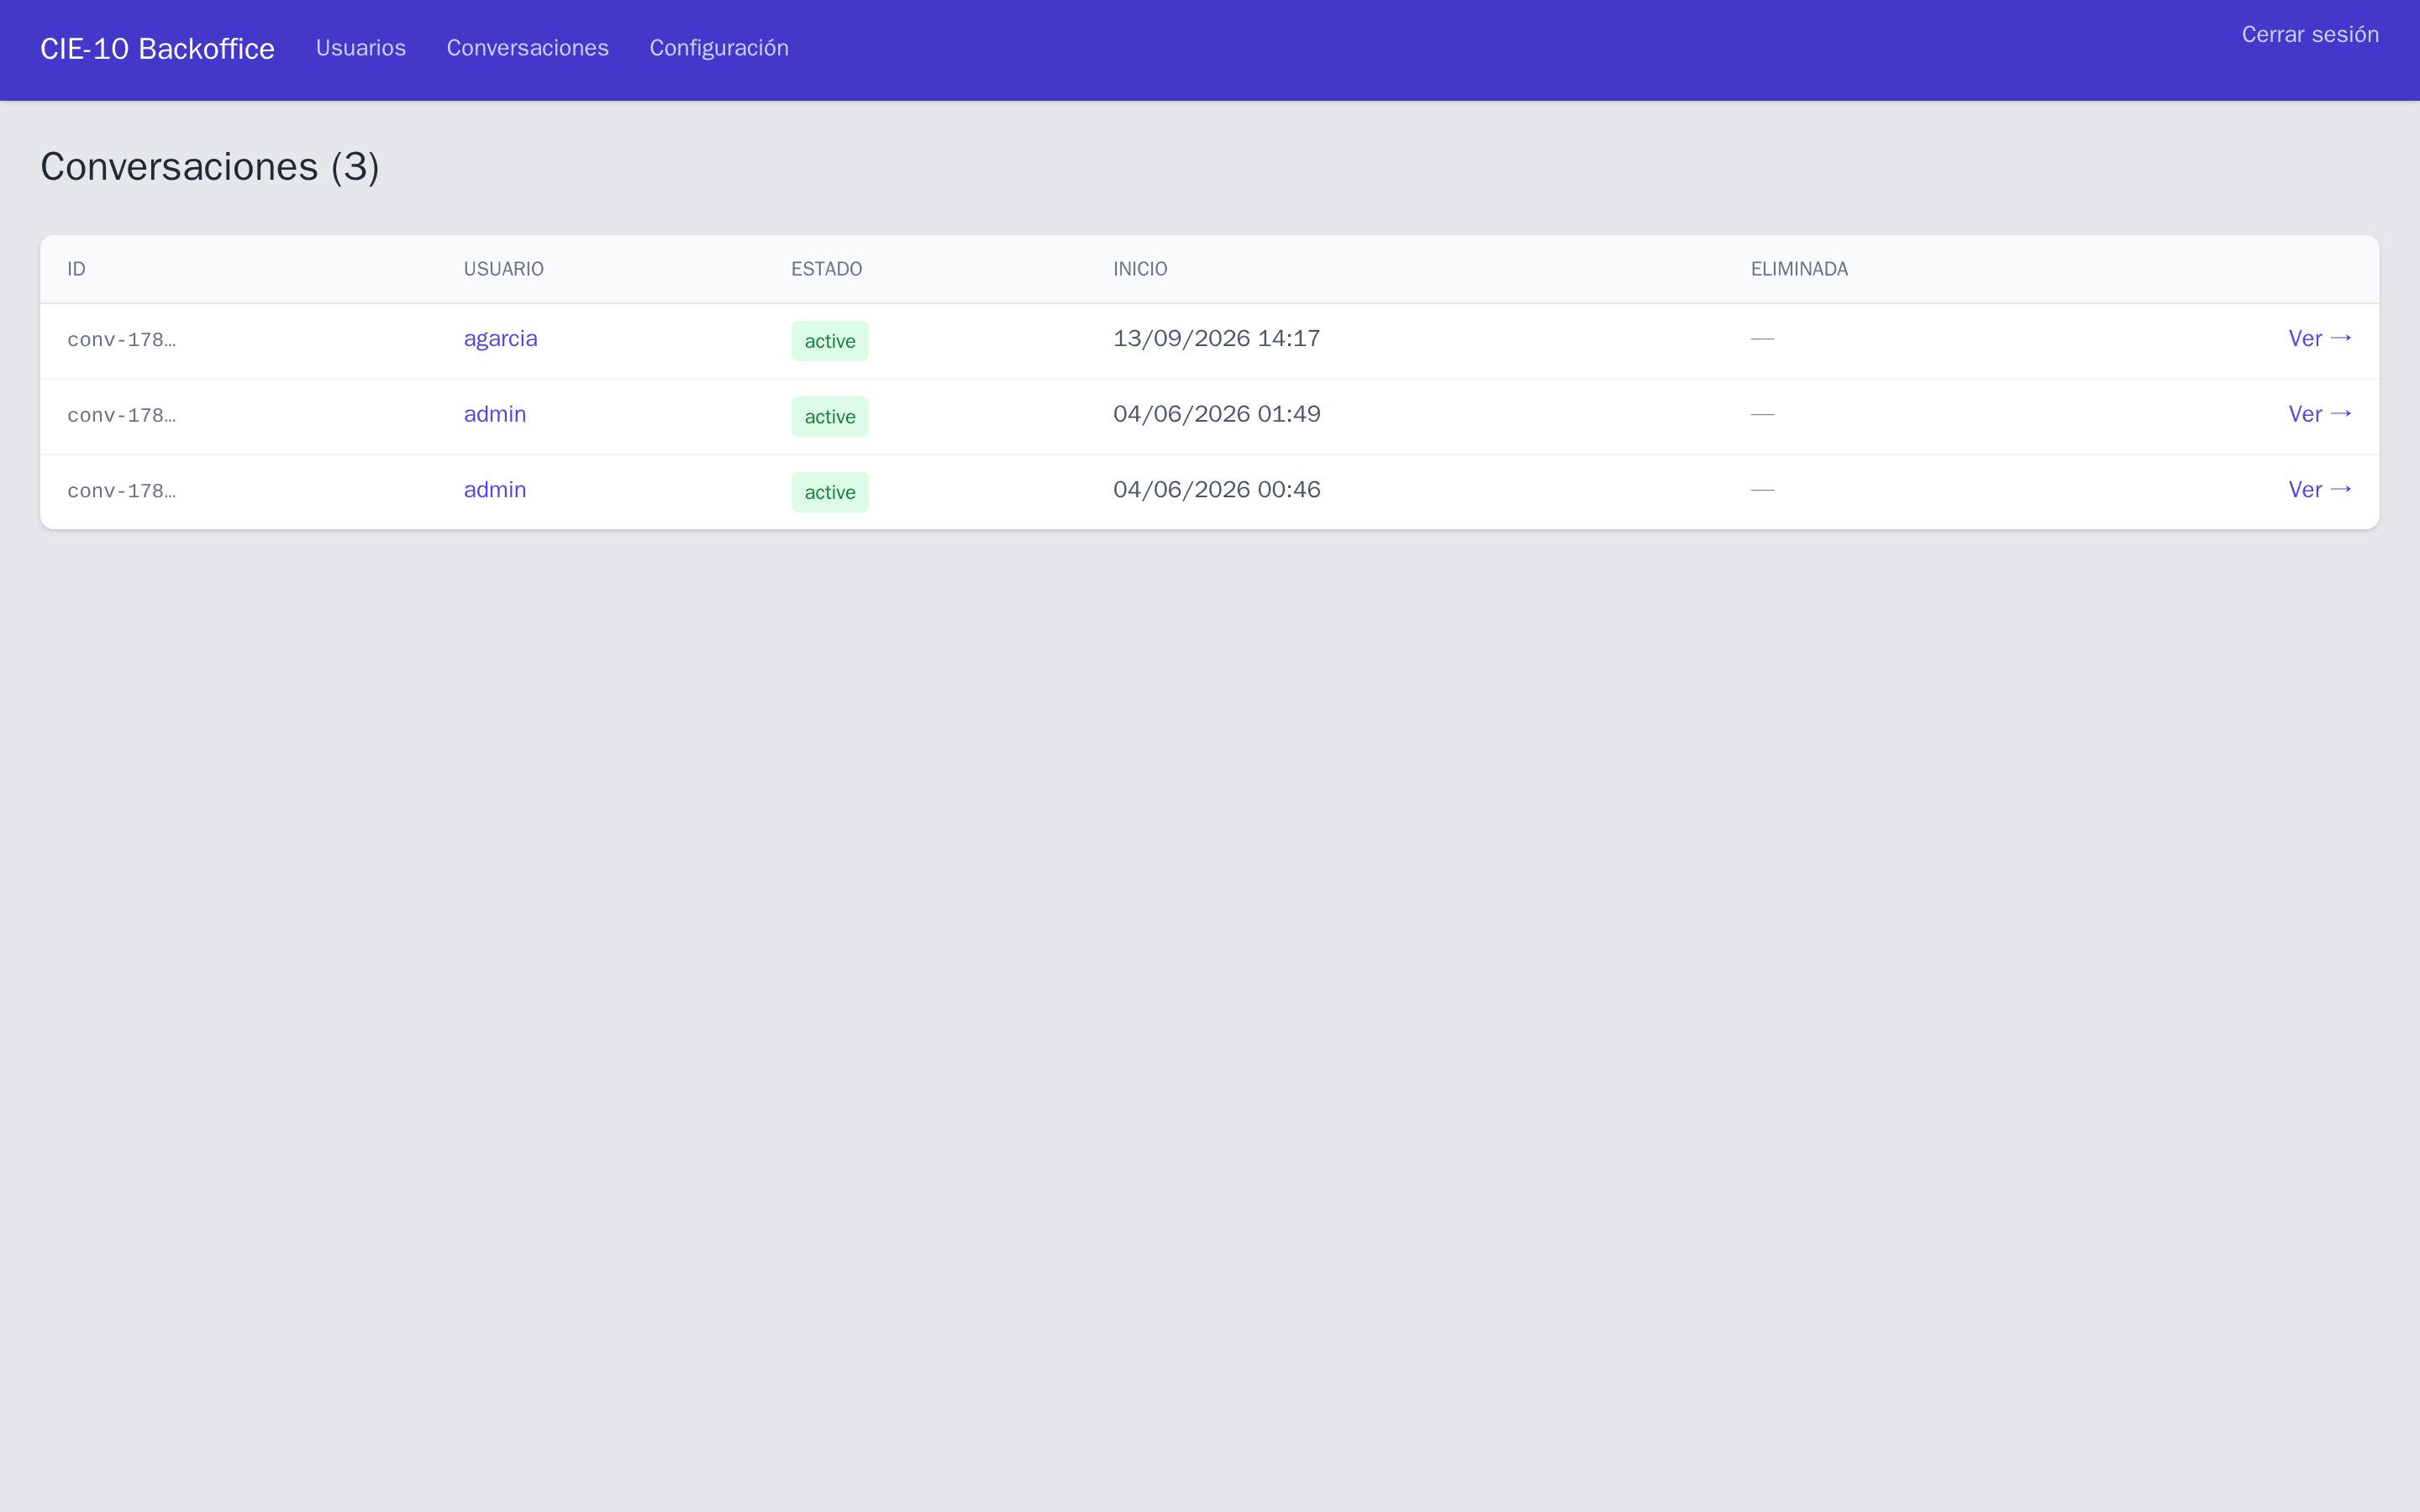
\includegraphics[width=0.9\textwidth, trim=0 1150 1180 0, clip]{figs/ui-admin-conversations}
\caption{Vista de administración de las conversaciones: cada análisis queda registrado con su usuario, estado y marca temporal, reflejo de la trazabilidad que aporta el \emph{Event Sourcing}.}
\label{fig:admin-conversations}
\end{figure}

\begin{figure}[ht]
\centering
\resizebox{\textwidth}{!}{% Diagrama de flujo CQRS / Event Sourcing
% Uso: % Diagrama de flujo CQRS / Event Sourcing
% Uso: \input{figs/cqrs-flujo} dentro de figure+\centering+\resizebox{\textwidth}{!}{...}
%
% Flujo: Comando → Manejador → Agregado → Evento → EventStore → Proyector → Modelo de lectura

\begin{tikzpicture}[
  every node/.style={font=\small\sffamily},
  %--- Escritura (lado izquierdo) ---
  cmd/.style={
    draw=palered!80, fill=palered!10, thick,
    rectangle, rounded corners=4pt,
    minimum width=2.6cm, minimum height=1.1cm,
    align=center
  },
  handler/.style={
    draw=gray!60, fill=gray!10, thick,
    rectangle, rounded corners=4pt,
    minimum width=2.6cm, minimum height=1.1cm,
    align=center
  },
  agg/.style={
    draw=aquaESI!80, fill=aquaESI!15, thick,
    rectangle, rounded corners=4pt,
    minimum width=2.6cm, minimum height=1.1cm,
    align=center
  },
  evt/.style={
    draw=ocre!80, fill=ocre!15, thick,
    rectangle, rounded corners=4pt,
    minimum width=2.6cm, minimum height=1.1cm,
    align=center
  },
  store/.style={
    draw=turquesa!80, fill=turquesa!15, thick,
    cylinder, shape border rotate=90,
    minimum height=1.4cm, minimum width=2.4cm,
    align=center
  },
  proj/.style={
    draw=gray!70, fill=gray!12, thick,
    rectangle, rounded corners=4pt,
    minimum width=2.6cm, minimum height=1.1cm,
    align=center
  },
  read/.style={
    draw=aquaESI!60, fill=aquaESI!10, thick,
    rectangle, rounded corners=4pt,
    minimum width=2.6cm, minimum height=1.1cm,
    align=center
  },
  %--- Flechas ---
  arr/.style={->, >=Stealth, thick},
  lbl/.style={font=\small\sffamily, midway, fill=white,
              inner sep=1.5pt, draw=gray!25, rounded corners=2pt},
  node distance=0.5cm and 0.9cm
]

%--- LADO ESCRITURA (fila superior) ---
\node[cmd] (cmd1) at (0,0) {
  \textbf{Comando}\\
  \footnotesize AnalyzeReport,\\ValidateCode
};

\node[agg, right=2.2cm of cmd1] (agg) {
  \textbf{Agregado}\\
  \footnotesize Analysis\\(estado)
};

\node[evt, right=2.0cm of agg] (evt1) {
  \textbf{Evento}\\
  \footnotesize ReportAnalyzed,\\CodeValidated
};

\node[store, right=2.2cm of evt1] (es) {
  \textbf{Event Store}\\
  \footnotesize PostgreSQL
};

%--- PROYECTOR (fila inferior) ---
\node[proj, below=1.4cm of es] (proj) {
  \textbf{Proyector}\\
  \footnotesize una proyección\\por evento
};

\node[read, left=1.2cm of proj, minimum width=5.4cm, text width=5.2cm] (r1) {
  \textbf{Modelo de lectura}\\
  \footnotesize conversations, analysis\_cards,\\predicted\_codes
};

%--- FLECHAS DE ESCRITURA ---
\draw[arr] (cmd1) -- node[lbl, above]{ejecuta} (agg);
\draw[arr] (agg)  -- node[lbl, above]{emite} (evt1);
\draw[arr] (evt1) -- node[lbl, above]{guarda} (es);

%--- FLECHA EventStore → Proyector ---
\draw[arr] (es) -- node[lbl, right]{se suscribe} (proj);

\draw[arr] (proj) -- node[lbl, above]{actualiza} (r1);

%--- ETIQUETAS DE ZONA ---
\node[font=\small\sffamily\bfseries, palered!80]
  at ($(cmd1)!0.5!(evt1) + (0,1.5)$) {Lado escritura (comandos)};

\node[font=\small\sffamily\bfseries, aquaESI!80]
  at ($(r1)!0.5!(proj) + (0,-1.5)$) {Lado lectura (consultas y proyecciones)};

%--- SEPARADOR ---
\draw[dashed, gray!50, thick]
  ($(es.south)!0.5!(proj.north)$) ++(-10,0) -- ++(13,0);

\end{tikzpicture}
 dentro de figure+\centering+\resizebox{\textwidth}{!}{...}
%
% Flujo: Comando → Manejador → Agregado → Evento → EventStore → Proyector → Modelo de lectura

\begin{tikzpicture}[
  every node/.style={font=\small\sffamily},
  %--- Escritura (lado izquierdo) ---
  cmd/.style={
    draw=palered!80, fill=palered!10, thick,
    rectangle, rounded corners=4pt,
    minimum width=2.6cm, minimum height=1.1cm,
    align=center
  },
  handler/.style={
    draw=gray!60, fill=gray!10, thick,
    rectangle, rounded corners=4pt,
    minimum width=2.6cm, minimum height=1.1cm,
    align=center
  },
  agg/.style={
    draw=aquaESI!80, fill=aquaESI!15, thick,
    rectangle, rounded corners=4pt,
    minimum width=2.6cm, minimum height=1.1cm,
    align=center
  },
  evt/.style={
    draw=ocre!80, fill=ocre!15, thick,
    rectangle, rounded corners=4pt,
    minimum width=2.6cm, minimum height=1.1cm,
    align=center
  },
  store/.style={
    draw=turquesa!80, fill=turquesa!15, thick,
    cylinder, shape border rotate=90,
    minimum height=1.4cm, minimum width=2.4cm,
    align=center
  },
  proj/.style={
    draw=gray!70, fill=gray!12, thick,
    rectangle, rounded corners=4pt,
    minimum width=2.6cm, minimum height=1.1cm,
    align=center
  },
  read/.style={
    draw=aquaESI!60, fill=aquaESI!10, thick,
    rectangle, rounded corners=4pt,
    minimum width=2.6cm, minimum height=1.1cm,
    align=center
  },
  %--- Flechas ---
  arr/.style={->, >=Stealth, thick},
  lbl/.style={font=\small\sffamily, midway, fill=white,
              inner sep=1.5pt, draw=gray!25, rounded corners=2pt},
  node distance=0.5cm and 0.9cm
]

%--- LADO ESCRITURA (fila superior) ---
\node[cmd] (cmd1) at (0,0) {
  \textbf{Comando}\\
  \footnotesize AnalyzeReport,\\ValidateCode
};

\node[agg, right=2.2cm of cmd1] (agg) {
  \textbf{Agregado}\\
  \footnotesize Analysis\\(estado)
};

\node[evt, right=2.0cm of agg] (evt1) {
  \textbf{Evento}\\
  \footnotesize ReportAnalyzed,\\CodeValidated
};

\node[store, right=2.2cm of evt1] (es) {
  \textbf{Event Store}\\
  \footnotesize PostgreSQL
};

%--- PROYECTOR (fila inferior) ---
\node[proj, below=1.4cm of es] (proj) {
  \textbf{Proyector}\\
  \footnotesize una proyección\\por evento
};

\node[read, left=1.2cm of proj, minimum width=5.4cm, text width=5.2cm] (r1) {
  \textbf{Modelo de lectura}\\
  \footnotesize conversations, analysis\_cards,\\predicted\_codes
};

%--- FLECHAS DE ESCRITURA ---
\draw[arr] (cmd1) -- node[lbl, above]{ejecuta} (agg);
\draw[arr] (agg)  -- node[lbl, above]{emite} (evt1);
\draw[arr] (evt1) -- node[lbl, above]{guarda} (es);

%--- FLECHA EventStore → Proyector ---
\draw[arr] (es) -- node[lbl, right]{se suscribe} (proj);

\draw[arr] (proj) -- node[lbl, above]{actualiza} (r1);

%--- ETIQUETAS DE ZONA ---
\node[font=\small\sffamily\bfseries, palered!80]
  at ($(cmd1)!0.5!(evt1) + (0,1.5)$) {Lado escritura (comandos)};

\node[font=\small\sffamily\bfseries, aquaESI!80]
  at ($(r1)!0.5!(proj) + (0,-1.5)$) {Lado lectura (consultas y proyecciones)};

%--- SEPARADOR ---
\draw[dashed, gray!50, thick]
  ($(es.south)!0.5!(proj.north)$) ++(-10,0) -- ++(13,0);

\end{tikzpicture}
}
\caption{Flujo CQRS/\emph{Event Sourcing} del backend: desde el comando hasta los modelos de lectura.}
\label{fig:cqrs-flujo}
\end{figure}

El almacenamiento de eventos se implementa sobre PostgreSQL, sin recurrir a una base de datos dedicada para \emph{Event Sourcing} como EventStoreDB o Apache Kafka. Esta decisión (ADR-04, Anexo~\ref{cap:AnexoE}) reduce la complejidad operativa: un único sistema de base de datos para administrar, con soporte nativo y maduro en Commanded. Si el volumen de eventos creciera hasta niveles que saturaran PostgreSQL, lo que en el contexto clínico de un hospital de tamaño medio no se prevé a corto plazo, la migración a un \emph{broker} de mensajes como Kafka es viable sin cambios estructurales en el dominio, gracias a la inversión de dependencias que aísla los agregados y proyectores del adaptador de persistencia concreto (principio DIP, detallado en la sección~\ref{sec:calidad}).

La comunicación en tiempo real entre frontend y backend se realiza mediante canales WebSocket de Phoenix, tecnología que encaja de forma natural con el modelo de actores de la BEAM. El canal \texttt{ConversationChannel} gestiona el envío de informes, la recepción asíncrona de predicciones del motor de IA y la difusión de tarjetas de análisis al cliente a medida que se generan, sin necesidad de sondeo periódico. La especificación completa de los mensajes WebSocket y de la API REST se recoge en el Anexo~\ref{cap:AnexoC}.

\subsection{Diseño del frontend}

El frontend está desarrollado en Next.js 16 con React 19 y TypeScript. La interfaz utiliza Tailwind CSS 4 y la biblioteca de componentes shadcn/ui. La arquitectura de estado se basa en contextos de React: \texttt{AuthContext} gestiona la sesión del usuario, \texttt{ConversationContext} gestiona el estado del análisis activo y el historial, e \texttt{I18nContext} gestiona las traducciones de la interfaz (cinco idiomas, sección~\ref{sec:i18n}).

La configuración de URLs de backend y WebSocket se centraliza en \texttt{src/lib/config.ts}, que lee las variables de entorno \texttt{NEXT\_PUBLIC\_API\_URL} y \texttt{NEXT\_PUBLIC\_WS\_URL}, evitando cualquier dirección codificada directamente en el código.

El punto de entrada a la aplicación es la pantalla de inicio de sesión (Figura~\ref{fig:ui-login}), desde la que el usuario accede al panel de análisis descrito en la sección~\ref{sec:modelo-interfaz}.

\begin{figure}[ht]
\centering
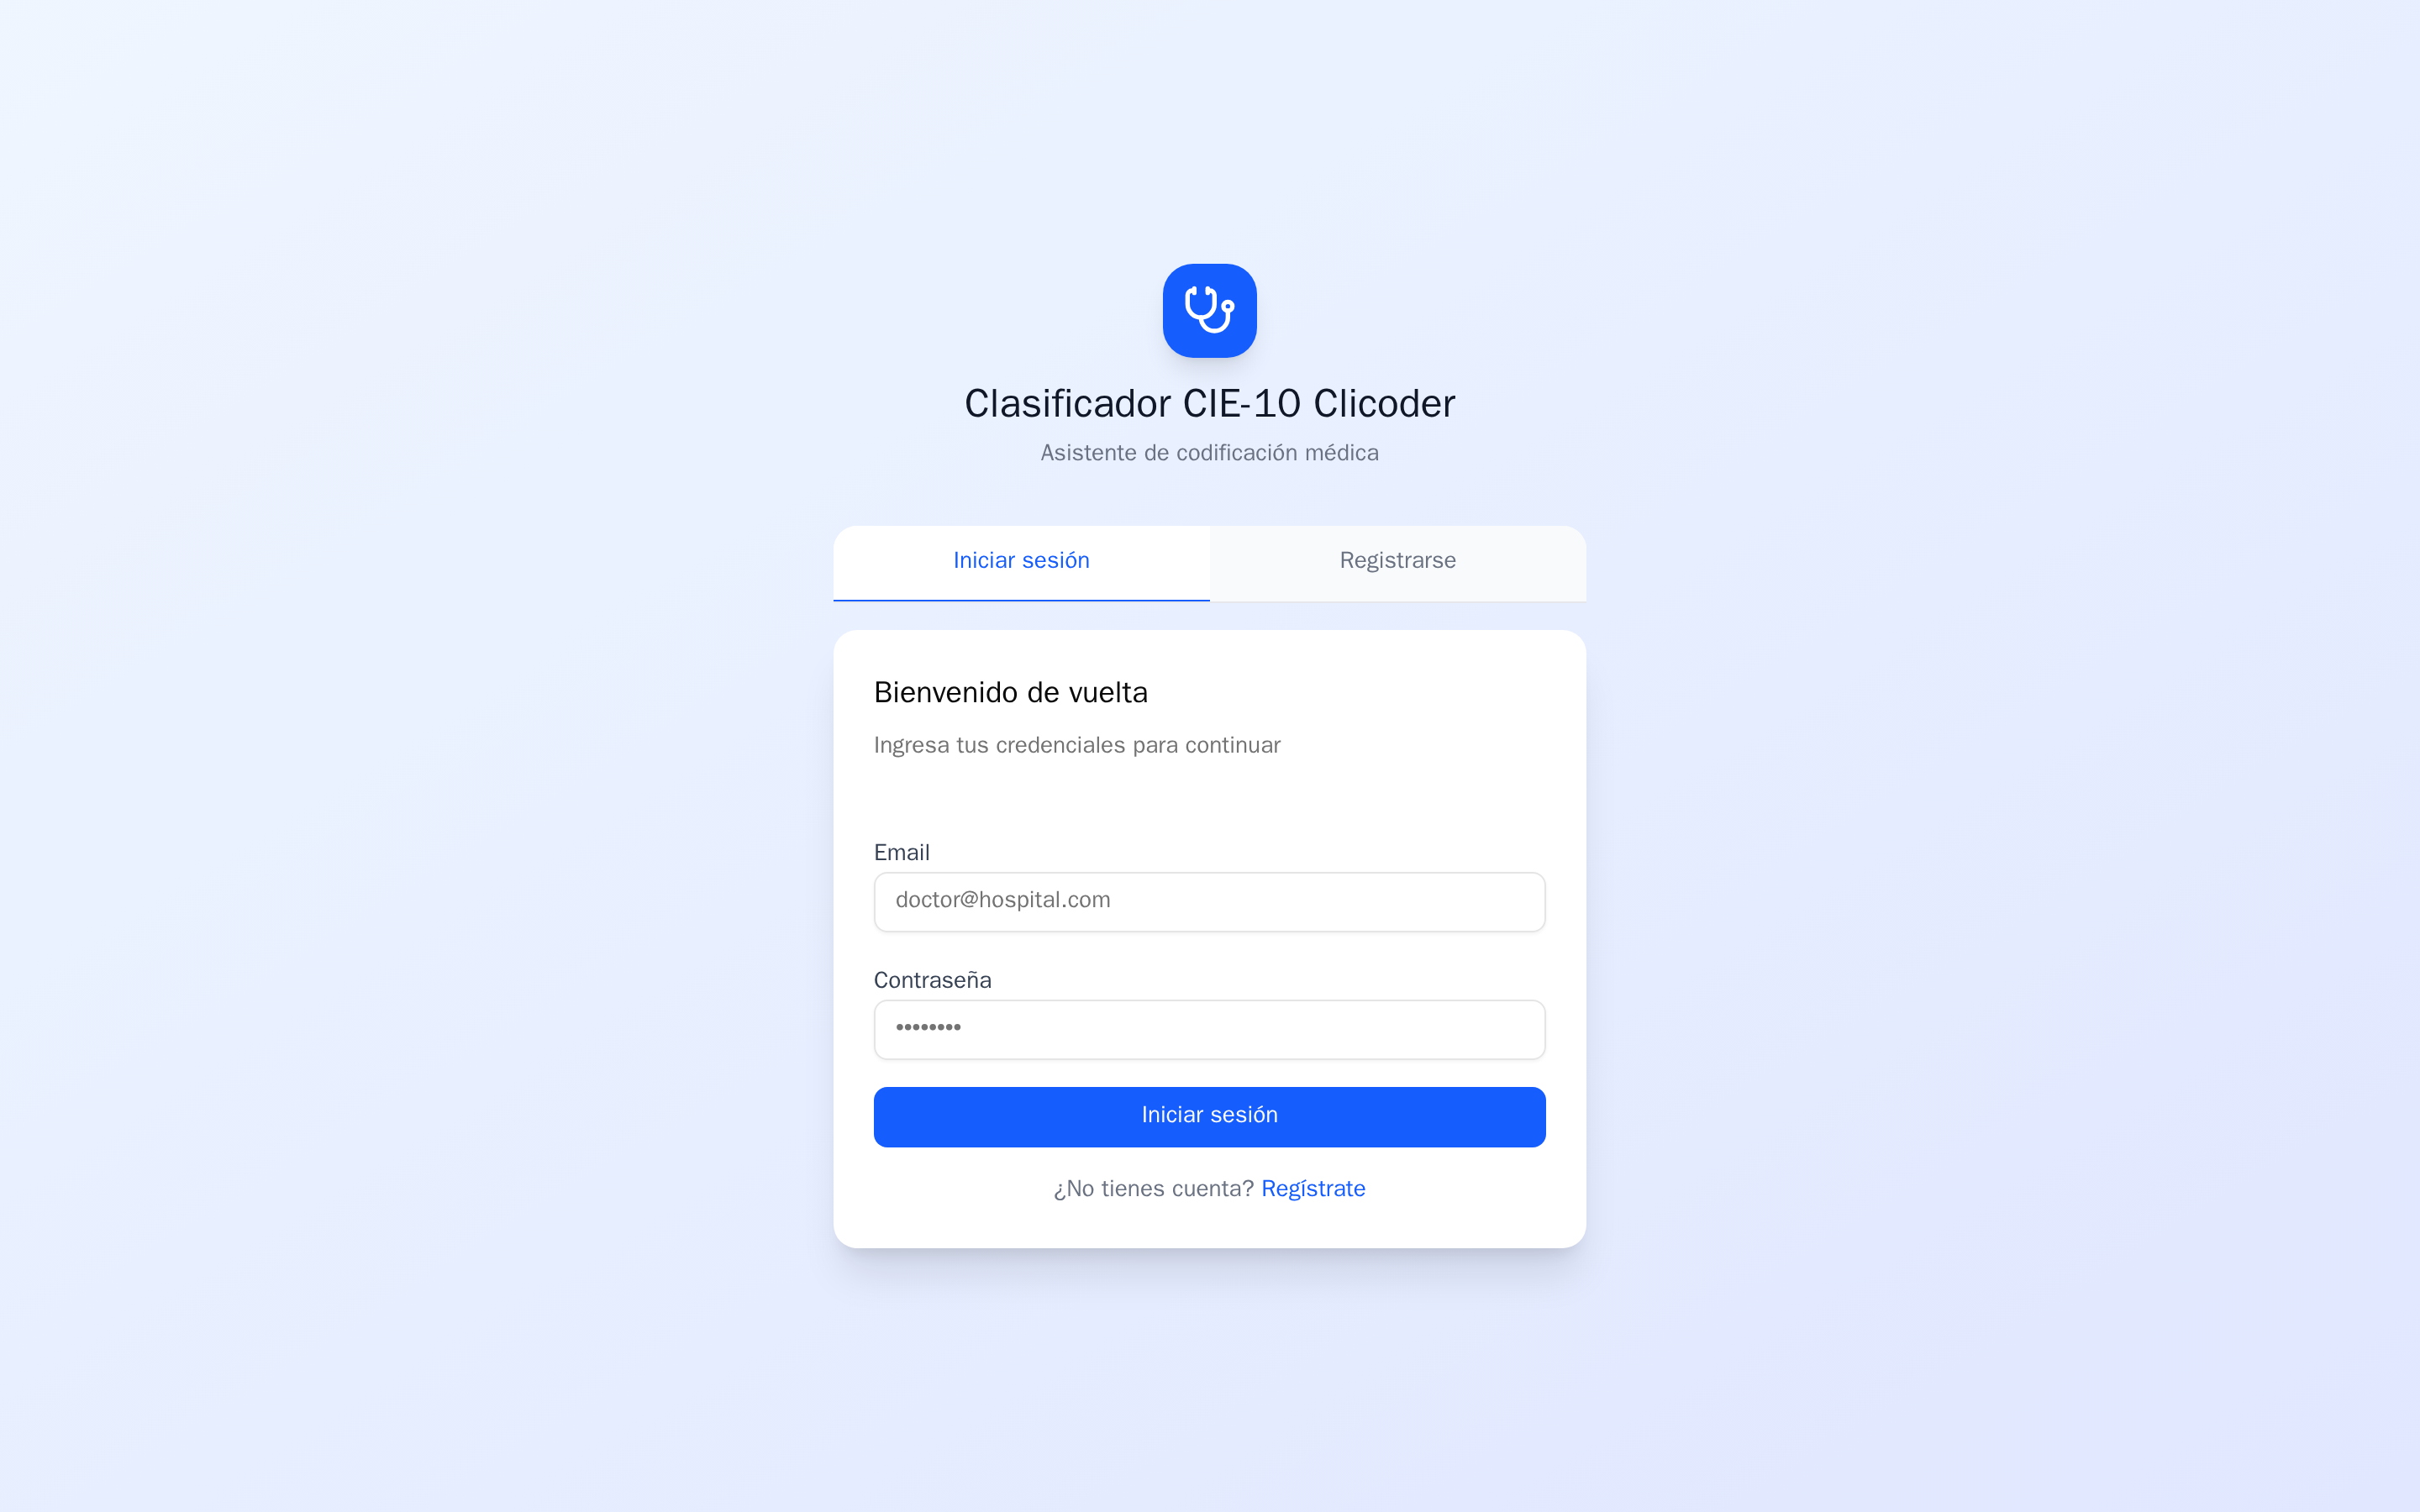
\includegraphics[width=0.45\textwidth, trim=920 270 920 270, clip]{figs/ui-login}
\caption{Pantalla de inicio de sesión de la interfaz web.}
\label{fig:ui-login}
\end{figure}

\section{Implementación del sistema}

\subsection{Estructura del repositorio}

El repositorio se organiza en los siguientes directorios de alto nivel:

\begin{itemize}
 \item \texttt{ai\_engine/}: servicio FastAPI de inferencia. Contiene el módulo \texttt{classifier.py} con la clase \texttt{CIE10Classifier}, el script de entrenamiento \texttt{train.py}, el punto de entrada \texttt{main.py} y los artefactos del modelo entrenado en \texttt{model/}.
 \item \texttt{ai\_engine\_mock/}: versión simulada del motor de IA para desarrollo local, que devuelve predicciones ficticias sin necesidad de cargar el modelo BERT.
 \item \texttt{backend/}: aplicación Phoenix. La lógica de negocio se organiza en \texttt{lib/app/} (contextos, agregados, proyectores) y la capa web en \texttt{lib/app\_web/} (controladores, canales, \emph{plugs}).
 \item \texttt{frontend/}: aplicación Next.js. Los componentes de UI están en \texttt{src/components/}, los contextos en \texttt{src/contexts/} y la lógica de comunicación en \texttt{src/lib/}.
 \item \texttt{training/}: entorno de entrenamiento separado del servicio de producción. Contiene los scripts de descarga de datos en \texttt{csv\_import\_scripts/}, los notebooks de análisis estadístico en \texttt{data\_analysis/} y los notebooks de entrenamiento en \texttt{bert-classifier/}.
\end{itemize}

El repositorio se gestiona con Git. El historial de commits refleja el desarrollo incremental del sistema y puede consultarse en el repositorio del proyecto.

\subsection{Pipeline de entrenamiento}

El entrenamiento del modelo se orquesta mediante el \texttt{Makefile} de la raíz del proyecto. El entrenamiento con GPU se lanza con \texttt{make ai-train-gpu} (con CPU, \texttt{make ai-train}) y deja los artefactos del modelo en el directorio \texttt{ai\_engine/model/}.

El script \texttt{train.py} acepta los siguientes parámetros configurables por línea de comandos: ruta a los ficheros de entrenamiento y validación, ruta al fichero de descripciones CIE-10-ES, directorio de salida, nombre del modelo base, longitud máxima de secuencia, número de épocas, tamaño de batch, acumulación de gradientes y dispositivo de cómputo. El modelo guarda un \emph{checkpoint} del mejor resultado en validación (por F1-micro), el mapeo código-índice y un fichero \texttt{config.json} con todos los hiperparámetros, de modo que la inferencia posterior no requiere conocer los parámetros de entrenamiento.

\subsection{Servicio de inferencia}

El servicio de inferencia (\texttt{ai\_engine/main.py}) es una aplicación FastAPI que carga el modelo BERT al arrancar mediante el mecanismo de ciclo de vida (\texttt{lifespan}). Expone los siguientes endpoints:

\begin{itemize}
 \item \texttt{POST /predict}: recibe el texto del informe y devuelve los códigos CIE-10 predichos. El resumen médico se genera por separado.
 \item \texttt{POST /summarize/stream}: genera el resumen o paráfrasis del informe en tiempo real, devolviendo los tokens del LLM de forma incremental mediante NDJSON (\emph{newline-delimited JSON}).
 \item \texttt{GET /}: comprueba que el servicio está en funcionamiento y que el modelo está cargado.
\end{itemize}

Si el directorio del modelo no existe al arrancar, el servicio se inicia igualmente y devuelve un error 503 en las peticiones de predicción, lo que facilita el desarrollo sin necesidad de tener el modelo entrenado.

\subsubsection{Módulo de generación de resúmenes}
\label{sec:resumidor}

Además de los códigos CIE-10, el sistema genera para cada informe un \textbf{resumen clínico} que acompaña a la propuesta de codificación y ayuda al codificador a situar rápidamente el caso. La generación se delega en un modelo de lenguaje generativo (LLM) ligero, independiente del clasificador, expuesto en el \emph{endpoint} \texttt{POST /summarize/stream}.

El modelo se ejecuta con \texttt{llama-cpp-python} sobre pesos cuantizados en formato GGUF (cuantización Q4\_K\_M), lo que permite servir el resumen \textbf{en CPU} sin GPU dedicada, en coherencia con la arquitectura de despliegue de bajo coste (Anexo~\ref{cap:AnexoI}). El modelo base es configurable, se evaluaron Gemma~3~4B, Gemma~E4B y E2B, Phi-4-mini y Qwen2.5-3B, con una ventana de contexto de 8.192 \emph{tokens}, suficiente para los informes del corpus. El componente admite dos modos: \texttt{summary}, que produce un resumen conciso (máximo 80 palabras), y \texttt{paraphrase}, que reformula el informe conservando todos los datos clínicos. El modelo activo, el modo y los \emph{prompts} de sistema y de usuario se ajustan en tiempo de ejecución desde el \emph{backoffice} de administración, sin necesidad de redesplegar (véase la sección~\ref{sec:feature-toggle}).

La generación emplea una temperatura baja (0,2) para favorecer salidas deterministas y fieles al texto original, y se emite token a token mediante \emph{streaming}, como se detalla en la sección~\ref{sec:streaming-resumen}. Al tratarse de una funcionalidad de apoyo (no forma parte del núcleo de codificación), el resumidor está desactivado por defecto en el despliegue de producción (\texttt{SUMMARIZER\_MODEL=none}) y se habilita bajo demanda, de modo que el coste computacional del LLM solo se asume cuando se desea esta ayuda.

\paragraph{Modelos evaluados.} El componente admite cinco modelos generativos ligeros, todos cuantizados a \texttt{Q4\_K\_M} y ejecutables en CPU (Tabla~\ref{tab:summarizer-modelos}). Ninguno es el modelo por defecto en producción: la variable \texttt{SUMMARIZER\_MODEL} se fija a \texttt{none} salvo que un administrador active uno desde el \emph{backoffice}.

\begin{table}[ht]
\centering
\small
\caption{Modelos generativos disponibles para el resumidor (GGUF, cuantización Q4\_K\_M, contexto de 8.192 \emph{tokens}).}
\label{tab:summarizer-modelos}
\begin{tabular}{lll}
\hline
\textbf{Clave} & \textbf{Modelo} & \textbf{Repositorio HuggingFace} \\
\hline
\texttt{gemma3}    & Gemma 3 4B IT       & \texttt{ggml-org/gemma-3-4b-it-GGUF} \\
\texttt{gemma4}    & Gemma 4 E4B IT      & \texttt{ggml-org/gemma-4-E4B-it-GGUF} \\
\texttt{gemma4-2b} & Gemma 4 E2B IT      & \texttt{ggml-org/gemma-4-E2B-it-GGUF} \\
\texttt{phi4}      & Phi-4 Mini Instruct & \texttt{bartowski/microsoft\_Phi-4-mini-instruct-GGUF} \\
\texttt{qwen}      & Qwen 2.5 3B Instruct & \texttt{Qwen/Qwen2.5-3B-Instruct-GGUF} \\
\hline
\end{tabular}
\end{table}

\paragraph{Prompts por defecto.} El comportamiento del modelo se controla mediante un \emph{prompt} de sistema y uno de usuario, ambos editables en caliente desde el \emph{backoffice} sin recargar el modelo. Los marcadores \texttt{\{text\}} (informe de entrada) y \texttt{\{language\}} (idioma de salida) se sustituyen en tiempo de ejecución. Los valores por defecto para cada modo son:

{\small
\begin{verbatim}
# Modo summary
sistema: "Médico CIE-10. Responde en {language}.
          Solo análisis, sin comentarios."
usuario: "Informe: {text}

          Resume (máx 80 palabras). Indica: diagnóstico, código CIE-10,
          palabras que lo activan y por qué.

          Análisis:"

# Modo paraphrase
sistema: "Médico CIE-10. Reformula conservando TODOS los datos médicos.
          Responde en {language}."
usuario: "Informe: {text}

          Reformula en prosa: motivo consulta, evolución, hallazgos,
          tratamiento. Al final: código CIE-10, palabras clave que lo
          activan, motivo.

          Reformulado:"
\end{verbatim}
}

\paragraph{Ejemplo ilustrativo.} Para el informe de demostración empleado en las capturas (véase la Figura~\ref{fig:ui-analysis}), el modo \texttt{summary} produce una salida del tipo:

\begin{quote}\small\itshape
Varón de 68 años con hipertensión arterial y diabetes mellitus tipo 2. Ingresa por infarto agudo de miocardio (dolor torácico opresivo, ECG y marcadores compatibles). Durante el ingreso desarrolla una neumonía nosocomial y un deterioro de la función renal compatible con enfermedad renal crónica. Códigos CIE-10 sugeridos: I21.9 (infarto agudo de miocardio), E11.9 (diabetes tipo 2), I10 (hipertensión), J18.9 (neumonía) y N18.9 (enfermedad renal crónica).
\end{quote}

El texto es una reformulación fiel del informe original: no introduce datos nuevos y sirve al codificador como resumen de contexto junto a los códigos propuestos por el clasificador.

El modelo activo, el modo y los \emph{prompts} se configuran desde el \emph{backoffice} de administración, sin necesidad de redesplegar (Figura~\ref{fig:admin-summarizer}).

\begin{figure}[ht]
\centering
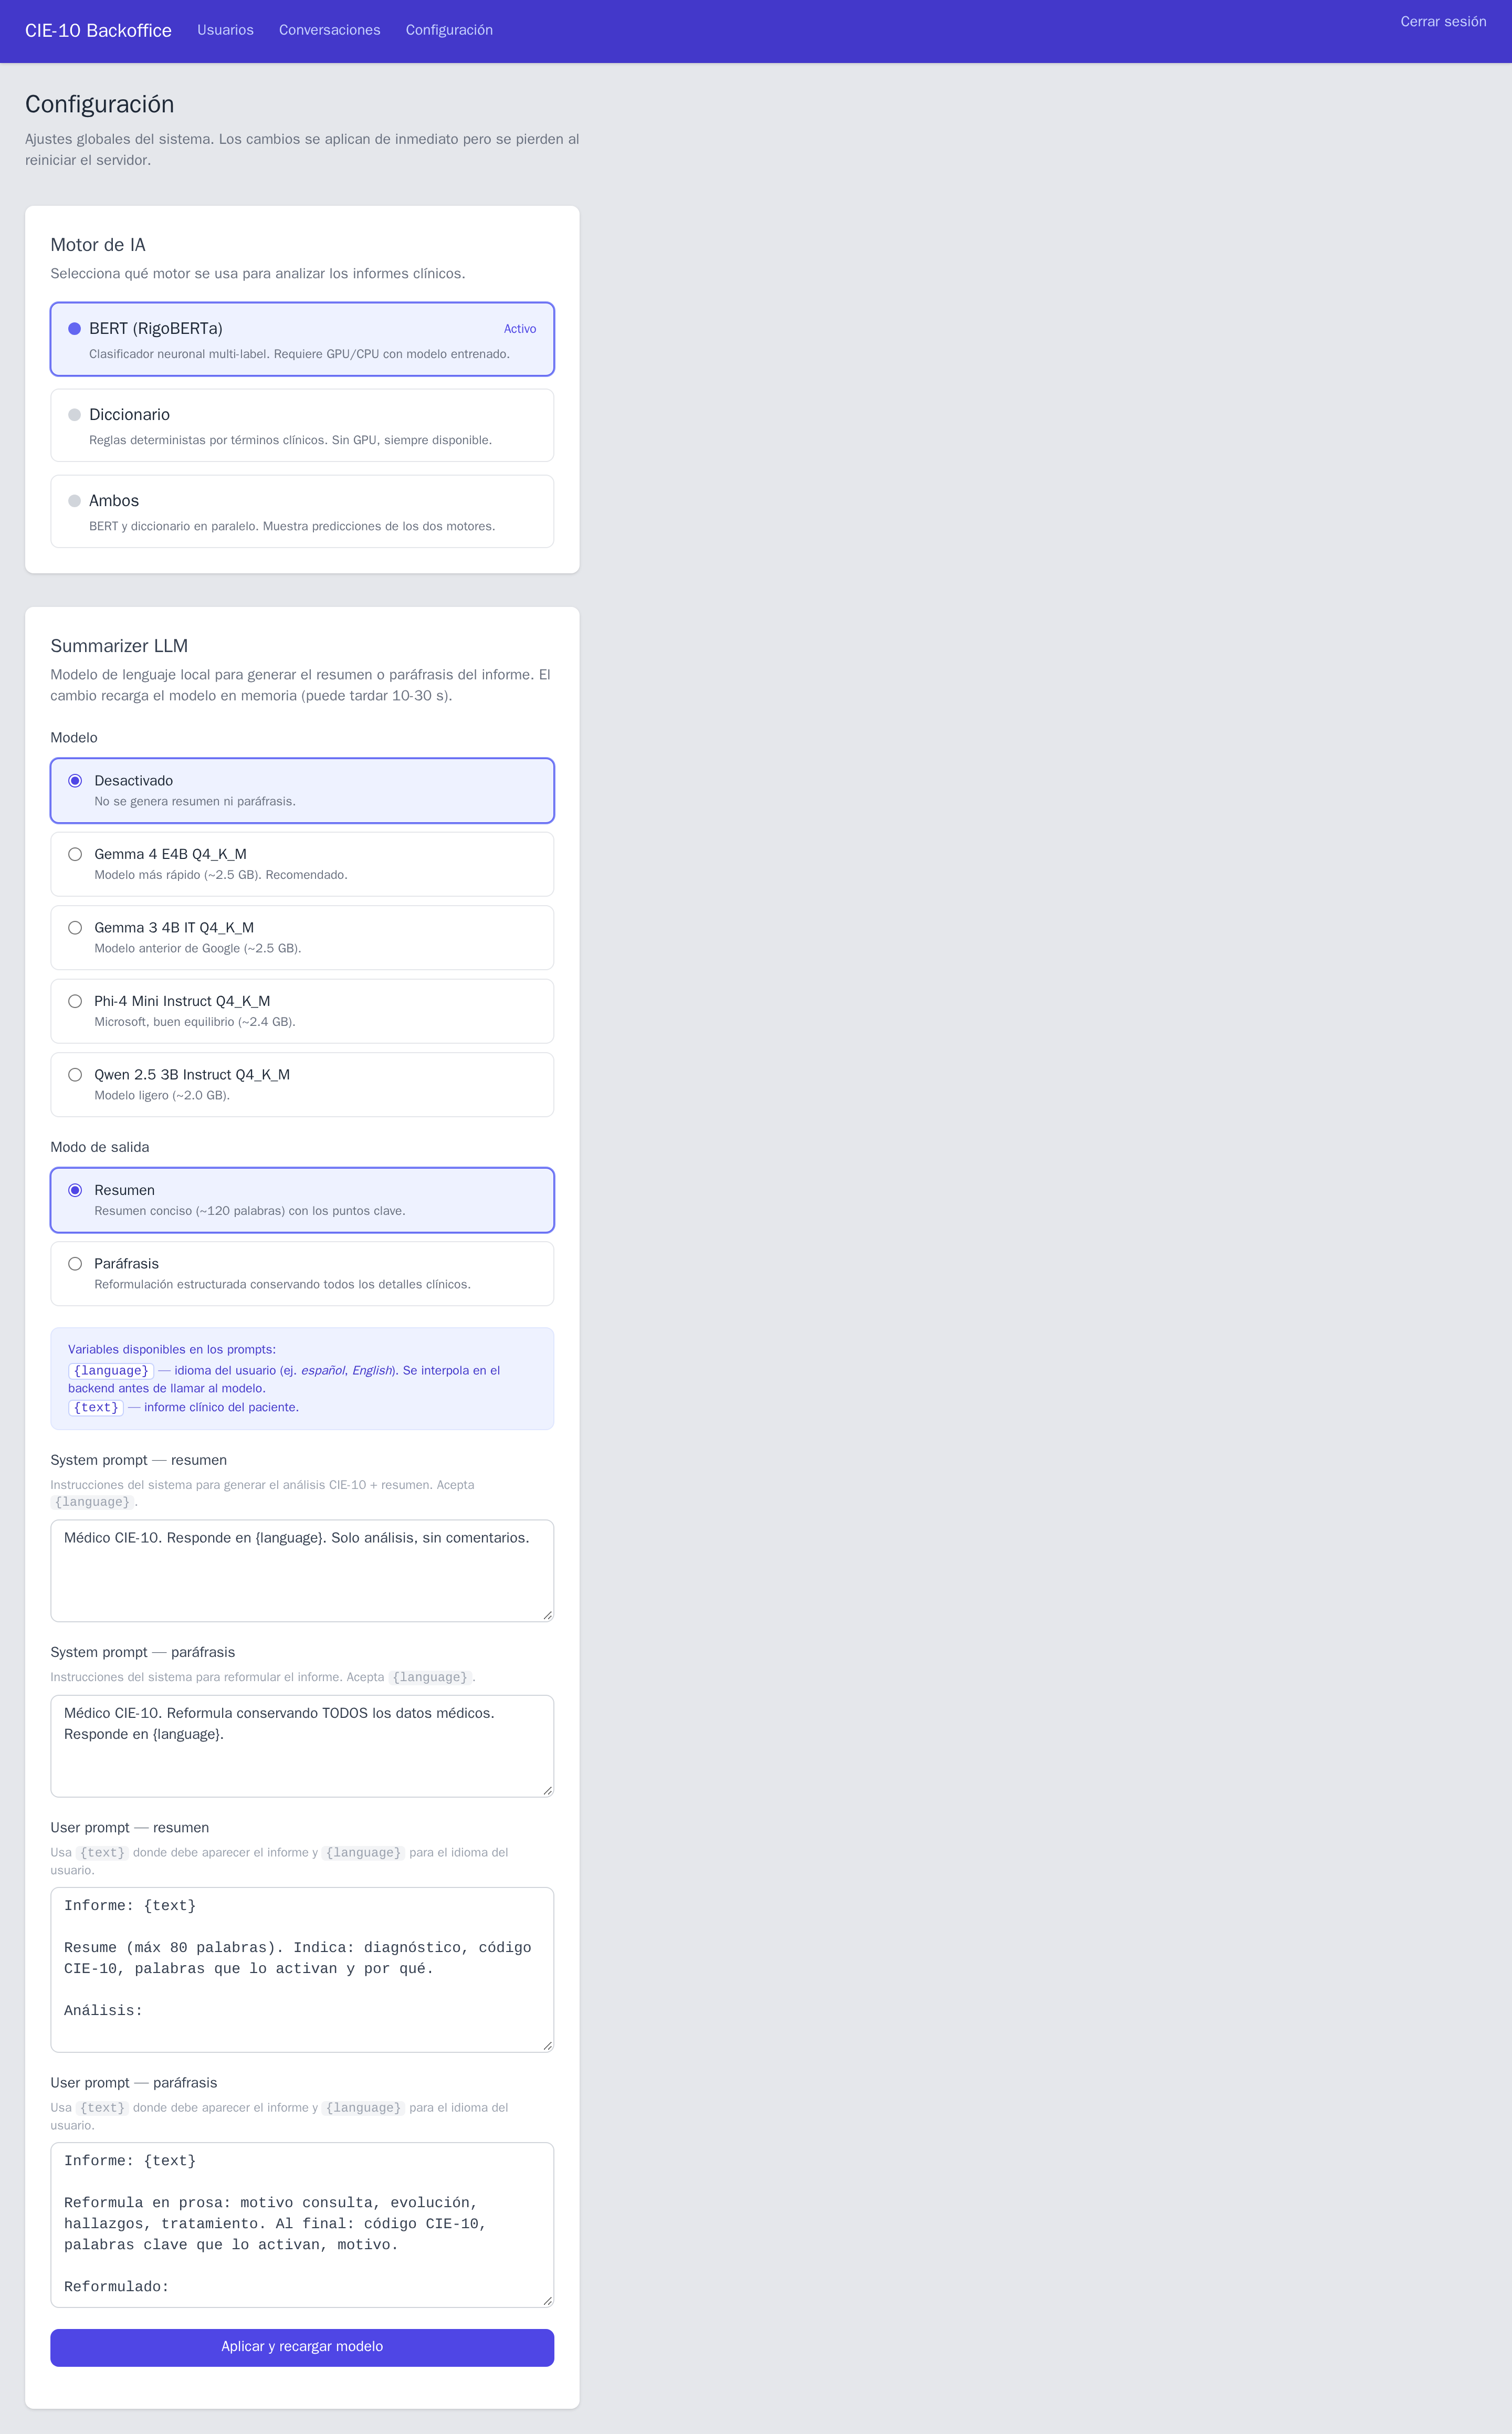
\includegraphics[width=0.75\textwidth, trim=35 2136 1770 1150, clip]{figs/ui-admin-settings}
\caption{Configuración del resumidor en el \emph{backoffice}: selección del modelo generativo (con su tamaño y recomendación) y del modo de salida (resumen o paráfrasis). Los \emph{prompts} de sistema y de usuario son editables en la misma página y se aplican en caliente.}
\label{fig:admin-summarizer}
\end{figure}

\subsubsection{Paralelización y \emph{streaming} del resumen}
\label{sec:streaming-resumen}

Un sistema de codificación clínica asistida debe minimizar la latencia percibida, especialmente cuando intervienen dos motores de inferencia con tiempos muy distintos: el clasificador BERT tarda entre 500\,ms y 2\,s, mientras que la generación del resumen por parte del LLM puede requerir entre 10\,s y 30\,s dependiendo del modelo y la longitud del informe.

La arquitectura adoptada separa ambas responsabilidades en llamadas independientes y las ejecuta en paralelo mediante dos tareas Elixir asíncronas (\texttt{Task.async}):

\begin{enumerate}
 \item \textbf{Predicción de códigos} (\texttt{POST /predict}): se lanza de inmediato y, en cuanto devuelve respuesta, los códigos se persisten y se emiten al cliente vía WebSocket con el evento \texttt{analysis\_card\_received}. El codificador puede empezar a revisar los códigos mientras el resumen se sigue generando.

 \item \textbf{Resumen en \emph{streaming}} (\texttt{POST /summarize/stream}): el LLM genera el resumen token a token usando \texttt{stream=True} de \texttt{llama-cpp-python}. Cada token se emite inmediatamente al cliente con el evento WebSocket \texttt{summary\_token}. El cliente muestra el texto progresivamente con un efecto \emph{typewriter}. Al completarse, se emite \texttt{analysis\_card\_received} con el texto íntegro para su persistencia en la base de datos.
\end{enumerate}

El tiempo total de espera para el usuario es $\max(t_{\text{predict}}, t_{\text{summarize}})$ en lugar de $t_{\text{predict}} + t_{\text{summarize}}$; en la práctica, los códigos aparecen varios segundos antes de que finalice el resumen. Esta mejora de la usabilidad sigue el principio de \emph{tiempo de respuesta percibido}: el usuario recibe información útil en cuanto está disponible, sin necesidad de esperar a que todos los componentes del análisis estén completos~\cite{Nielsen94}.

El \emph{streaming} del resumen presenta además una ventaja psicológica: el usuario observa que el sistema está procesando activamente su consulta, lo que reduce la sensación de espera incluso cuando el tiempo total es idéntico. Este efecto está documentado en la literatura de interacción persona-ordenador bajo el concepto de retroalimentación de progreso~\cite{Harrison07}.

\subsubsection{Selección del motor de IA mediante \emph{feature toggle}}
\label{sec:feature-toggle}

El parámetro \texttt{engine} del endpoint \texttt{POST /predict} actúa como un \textbf{\emph{feature toggle}} o \emph{feature flag}: permite seleccionar en tiempo de ejecución, sin modificar ni desplegar código, qué motor de predicción utiliza el sistema. Los valores admitidos son \texttt{\textquotedbl{}bert\textquotedbl{}} (clasificador neuronal RigoBERTa, valor por defecto), \texttt{\textquotedbl{}dict\textquotedbl{}} (clasificador de diccionario determinista) \texttt{\textquotedbl{}both\textquotedbl{}} (ambos motores en paralelo, devolviendo las predicciones de cada uno con su campo \texttt{\textquotedbl{}engine\textquotedbl{}} identificando el origen) y \texttt{\textquotedbl{}fused\textquotedbl{}} (un único \emph{ranking} en el que la confianza del diccionario suma al \emph{logit} del modelo antes de ordenar).

Un \emph{feature toggle}~\cite{Fowler17} es una técnica de ingeniería del software que separa la \emph{activación} de una funcionalidad de su \emph{despliegue}. El código de la funcionalidad llega a producción desactivado, o activable dinámicamente, y se habilita o conmuta sin necesidad de relanzar el servicio. En contraste con los \emph{feature branches}, que retrasan la integración del código, los \emph{feature toggles} permiten integración continua: la rama principal contiene siempre el código más actualizado y son los \emph{feature toggles} quienes determinan qué comportamiento observan los usuarios en cada momento.

En este proyecto, el \emph{feature toggle} se implementa en dos capas:

\begin{itemize}
 \item \textbf{Motor de IA (Python / FastAPI)}: el parámetro \texttt{engine} del cuerpo JSON de \texttt{POST /predict} determina qué función interna se invoca: \texttt{\_predict\_bert}, \texttt{\_predict\_dict}, \texttt{\_predict\_both} o \texttt{\_predict\_fused}. Cuando se elige \texttt{\textquotedbl{}both\textquotedbl{}}, ambas funciones se ejecutan en paralelo con \texttt{asyncio.gather} y sus resultados se concatenan, preservando el campo \texttt{\textquotedbl{}engine\textquotedbl{}} de cada predicción para que la interfaz pueda distinguir el origen de cada código.

 \item \textbf{Backend (Elixir / Phoenix)}: el módulo \texttt{App.AIEngineSettings} es un proceso \texttt{Agent} de OTP que mantiene el valor activo del selector en memoria. Al arrancar el nodo BEAM, el agente se inicializa con \texttt{\textquotedbl{}bert\textquotedbl{}} como valor por defecto. El canal WebSocket \texttt{ConversationChannel} consulta \texttt{AIEngineSettings.get\_engine/0} en cada análisis y envía el valor al motor de IA como parte del cuerpo de la petición HTTP.
\end{itemize}

El selector se expone en el \emph{backoffice} de administración (\texttt{/admin/settings}), implementado como una página LiveView interactiva (Figura~\ref{fig:admin-settings}). Al hacer clic en una de las cuatro opciones, el evento se envía mediante WebSocket al servidor sin recargar la página, y el backend actualiza el \texttt{Agent} de forma inmediata. El cambio es \textbf{volátil}: si el servidor se reinicia, el valor vuelve al valor por defecto (\texttt{\textquotedbl{}bert\textquotedbl{}}), comportamiento intencionado dado que el selector sirve para comparar motores durante la evaluación del sistema, no como configuración permanente. El selector de estrategia de explicabilidad, en cambio, \textbf{sí se persiste} en la tabla de ajustes. La asimetría es deliberada: el motor es un instrumento de evaluación, mientras que la estrategia de atribución es una elección de calidad y coste que debe sobrevivir a un reinicio, porque de lo contrario el sistema cambiaría de comportamiento sin que nadie lo hubiera tocado.

\begin{figure}[ht]
\centering
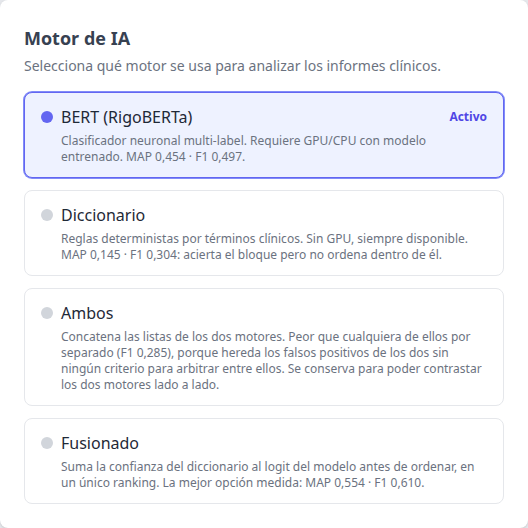
\includegraphics[width=0.7\textwidth]{figs/ui-admin-motor}
\caption{\emph{Backoffice} de administración (\texttt{/admin/settings}): selección del motor de IA entre las cuatro opciones disponibles, aplicable en caliente sin redesplegar.}
\label{fig:admin-settings}
\end{figure}

\paragraph{Selección del modelo desplegado.}
El mismo panel permite además cambiar el \emph{checkpoint} que sirve el clasificador. El motor de IA expone su catálogo en \texttt{GET /admin/models} y acepta cargar otro en caliente con \texttt{POST /admin/models}, sin reiniciar el servicio. El panel consulta ese catálogo al abrirse y presenta cada modelo con su descripción, sus métricas comparables y dos indicadores que conviene distinguir: si está \emph{cargado} y si está \emph{descargado} (Figura~\ref{fig:admin-modelo}). Un modelo del catálogo puede no estar en disco, porque cada \emph{checkpoint} ocupa algo más de 2\,GB y se obtiene por separado con \texttt{make model-download}; sin ese aviso, intentar activarlo fallaría sin explicación, de modo que la acción de carga solo se ofrece sobre los que están presentes.

\begin{figure}[ht]
\centering
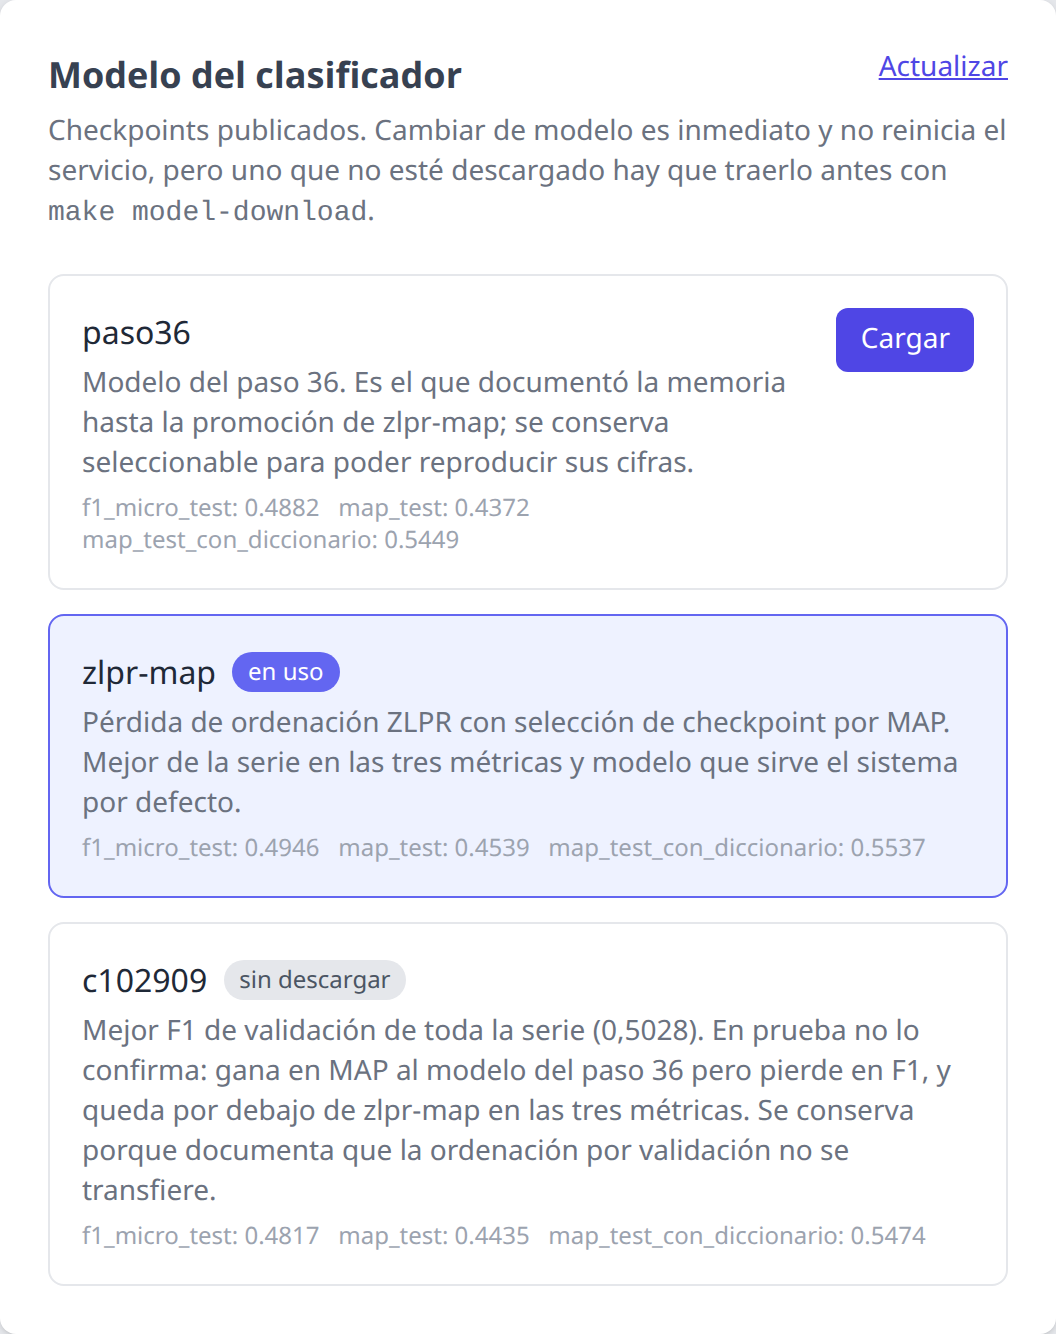
\includegraphics[width=0.65\textwidth]{figs/ui-admin-modelo}
\caption[Selector de modelo del clasificador]{Selector de modelo del clasificador. Cada \emph{checkpoint} muestra sus métricas comparables y dos indicadores independientes: cuál está en uso y cuál está descargado. La acción de carga solo se ofrece sobre los que están presentes en disco.}
\label{fig:admin-modelo}
\end{figure}

La consulta del catálogo se hace de forma tolerante a fallos: si el motor de IA no responde, el panel se abre igualmente y muestra el error en lugar de quedarse en blanco. La razón es práctica, y es la misma que justifica el selector de motores: el panel es justamente donde se cambia de configuración cuando algo va mal, así que no puede depender de que el componente que falla esté disponible.


Esta arquitectura sigue el principio de diseño \emph{«separación de responsabilidades»}: el motor de IA no sabe nada del mecanismo de selección, simplemente atiende la petición que recibe; el backend actúa como orquestador y centraliza la decisión de qué motor invocar; y la interfaz de administración proporciona el punto de control sin acoplarse a la lógica de predicción.

\subsubsection{Representación de la confianza de las predicciones}
\label{sec:confianza-predicciones}

\paragraph{El problema.}
Las probabilidades devueltas por un clasificador multi-label entrenado con \texttt{BCEWithLogitsLoss} son, en general, difíciles de interpretar directamente como porcentajes de confianza. La función de activación \emph{sigmoid} mapea el logit de cada clase al intervalo $(0, 1)$, y durante el entrenamiento el modelo es penalizado por alejarse de los valores objetivo $\{0, 1\}$. Como consecuencia, las predicciones positivas que superan el umbral de decisión tienden a concentrarse en el extremo superior del rango, típicamente entre 0{,}80 y 0{,}99, mientras que las negativas se agrupan cerca de 0. Mostrar este valor directamente al usuario como un porcentaje produce una interfaz poco informativa: casi todos los códigos predichos aparecen con una confianza superior al 90\,\%, lo que impide al codificador clínico priorizar rápidamente los diagnósticos más probables.

\paragraph{Causa raíz.}
El fenómeno es inherente a la calibración del modelo. Un clasificador entrenado únicamente para minimizar la pérdida de entropía cruzada binaria no garantiza que las probabilidades de salida estén calibradas en sentido estadístico~\cite{Guo17}. La solución canónica, \emph{temperature scaling} o calibración de Platt, requeriría un conjunto de validación adicional y añade un hiperparámetro más al ciclo de entrenamiento, lo que excede el alcance de este proyecto.

\paragraph{Solución adoptada: normalización relativa en tiempo de inferencia.}
En lugar de calibrar el modelo, se optó por normalizar las puntuaciones dentro del propio conjunto de predicciones devueltas en cada consulta. Dado un conjunto de $n$ códigos predichos con probabilidades $p_1 \geq p_2 \geq \cdots \geq p_n$, se define la \emph{confianza relativa} de cada código como:

\begin{equation}
 r_i = \frac{p_i - p_n}{p_1 - p_n}, \quad i = 1, \ldots, n
\end{equation}

donde $p_1$ es la probabilidad máxima y $p_n$ la mínima del conjunto. Si todos los valores son iguales ($p_1 = p_n$), se asigna $r_i = 1$ a todos. Este valor $r_i \in [0, 1]$ no representa una probabilidad calibrada, sino la \textbf{fortaleza relativa} de cada predicción respecto a las demás en esa misma consulta.

La normalización se aplica en el servicio de inferencia (\texttt{ai\_engine}) inmediatamente después de construir la lista de predicciones, tanto para el motor BERT como para el clasificador de diccionario, y se incluye en la respuesta como campo \texttt{relative\_confidence} junto a la probabilidad bruta original.

\paragraph{Representación visual.}
En el \emph{frontend}, la confianza relativa se muestra como una barra de progreso de ancho proporcional a $r_i$, con código de color en tres tramos: verde ($r_i \geq 0{,}66$), amarillo ($0{,}33 \leq r_i < 0{,}66$) y naranja ($r_i < 0{,}33$). La probabilidad bruta se conserva visible como texto secundario de pequeño tamaño, de forma que el codificador avanzado pueda consultarla si lo necesita. Esta combinación permite distinguir con rapidez qué códigos tienen mayor respaldo del modelo dentro de cada análisis, sin inducir una falsa precisión numérica.

\subsubsection{Explicabilidad de las predicciones}
\label{sec:explicabilidad}

La explicabilidad (\emph{explainability}) de los sistemas de aprendizaje automático es especialmente relevante en el ámbito clínico, donde el usuario necesita comprender \emph{por qué} el modelo sugiere un determinado código antes de validarlo. Sin esta información, el sistema actúa como una caja negra y dificulta la supervisión médica~\cite{Arrieta20}.

\paragraph{Limitaciones de la atención como explicación.}
Una primera aproximación natural sería utilizar los pesos de atención del transformador: los tokens a los que el mecanismo de atención presta más importancia en la capa final podrían interpretarse como los fragmentos más relevantes del informe. Sin embargo, Jain y Wallace~\cite{Jain19} demostraron empíricamente que los pesos de atención no son explicaciones fiables en el sentido de la teoría de la interpretabilidad: es posible obtener predicciones idénticas con distribuciones de atención muy distintas, y los tokens más atendidos no son necesariamente los responsables de la decisión. Por tanto, aunque los pesos de atención son útiles como herramienta de diagnóstico del modelo, no deben presentarse al usuario final como justificación de las predicciones.

\paragraph{Primera aproximación: Gradient $\times$ Input y su descarte.}
La primera implementación adoptó \textbf{Gradient~$\times$~Input}~\cite{Simonyan14}: para cada código $k$ y token $i$, se calculaba $s_{i,k} = |\nabla_{\mathbf{e}_i}\ell_k \odot \mathbf{e}_i|_1$ mediante una pasada hacia atrás desde el logit del código hasta los embeddings de entrada. El método es post-hoc, no requiere reentrenamiento y tiene coste $O(|\mathcal{P}|)$ pasadas backward para un conjunto de predicciones $\mathcal{P}$.

Sin embargo, la evaluación empírica sobre informes clínicos reales reveló atribuciones de escasa utilidad. En un informe que contenía el término \emph{brucelosis} y para el que el modelo predijo correctamente el código de brucelosis (A23), el método no identificó \emph{brucelosis} entre los tokens de mayor saliencia. Este comportamiento se repitió con otros términos clínicos específicos en las pruebas realizadas: el gradiente al propagarse hacia atrás por las 24 capas del \emph{encoder} RigoBERTa-Clinical se difumina hasta asignar saliencias comparables a términos clínicos y a artículos o preposiciones. El problema es inherente a arquitecturas transformer profundas con pooling en el token \texttt{[CLS]}: el gradiente debe atravesar todos los mecanismos de atención antes de llegar a los embeddings, perdiendo especificidad por el camino.

\paragraph{Método adoptado: atribución por enmascaramiento (\emph{masking perturbation}).}
Descartado el enfoque de gradientes, se adoptó la \textbf{atribución por perturbación}: para cada palabra $w$ del informe y cada código predicho $k$, se mide el descenso en el logit $\ell_k$ al sustituir los tokens de $w$ por el token especial \texttt{[MASK]}:

\begin{equation}
 s_{w,k} = \max\!\left(0,\; \ell_k(\mathbf{x}) - \ell_k(\mathbf{x}_{w \to \text{[MASK]}})\right)
\end{equation}

donde $\mathbf{x}_{w \to \text{[MASK]}}$ es la secuencia de entrada con los tokens de la palabra $w$ reemplazados por \texttt{[MASK]}. Un valor alto de $s_{w,k}$ indica que eliminar $w$ reduce significativamente la confianza del modelo en el código $k$: $w$ es un término clave para esa predicción concreta. Solo se evalúan palabras de cuatro o más caracteres para evitar ruido de stopwords y artículos. Este método mide directamente el \textbf{impacto causal} de cada palabra sobre la predicción, produciendo atribuciones fiables incluso en redes profundas donde los gradientes se difuminan.

La Figura~\ref{fig:ejemplo-explicabilidad} muestra el resultado sobre un informe real del conjunto de prueba, generada con \texttt{ai\_engine/figura\_explicabilidad.py}. El ejemplo sirve para ver a la vez lo que el método consigue y dónde falla: entre los cinco términos que más sostienen el código de dependencia del tabaco aparece \emph{cigarrillos}, que es la evidencia que un codificador buscaría, junto a otras cuatro palabras (\emph{posteriormente}, \emph{micciones}, \emph{persistente}, \emph{normales}) sin relación con ese diagnóstico. La atribución mide una dependencia real del \emph{logit}, no una justificación clínica: si el modelo se apoya en una palabra irrelevante, el método la señala con la misma honestidad con que señala la correcta. Esa es precisamente su utilidad para revisar predicciones, y la razón por la que la interfaz presenta los términos como pistas y no como argumentos.

% Generado por ai_engine/figura_explicabilidad.py: no editar a mano.
\begin{figure}[ht]
\centering
\fbox{\parbox{0.93\textwidth}{\footnotesize\setlength{\baselineskip}{13pt}
Paciente de 70 años de edad, minero jubilado, sin alergias medicamentosas conocidas, que presenta como antecedentes personales: accidente laboral antiguo con fracturas vertebrales y costales; intervenido de enfermedad de Dupuytren en mano derecha y by-pass iliofemoral izquierdo; Diabetes Mellitus tipo II, \colorbox{amarillo!14}{hipercolesterolemia} e hiperuricemia; enolismo activo, fumador de 20 \colorbox{amarillo!45}{cigarrillos} / día. Es derivado desde Atención Primaria por presentar hematuria macroscópica postmiccional en una ocasión y microhematuria \colorbox{amarillo!14}{persistente} \colorbox{amarillo!28}{posteriormente,} con \colorbox{amarillo!28}{micciones} \colorbox{amarillo!14}{normales.} En la exploración física presenta un buen estado general, con abdomen y genitales \colorbox{amarillo!14}{normales;} tacto rectal compatible con
}}
\caption[Ejemplo de explicabilidad sobre un informe real]{Términos que sostienen la predicción
del código \texttt{F17.210} (Dependencia de nicotina, cigarrillos, sin complicaciones) sobre un informe del conjunto de
prueba. El sombreado es proporcional a la caída del \emph{logit} al enmascarar cada palabra,
en tres niveles. Los cinco primeros: \emph{cigarrillos} (0,41), \emph{posteriormente} (0,16), \emph{micciones} (0,14), \emph{persistente} (0,12), \emph{normales} (0,11).}
\label{fig:ejemplo-explicabilidad}
\end{figure}


\paragraph{Implementación.}
La atribución se calcula en el método \texttt{CIE10Classifier.explain()} (\texttt{ai\_engine/classifier.py}):

\begin{enumerate}
 \item Se tokeniza el texto y se obtiene el mapeo palabra~$\to$~posiciones de subword tokens mediante \texttt{word\_ids()} del tokenizador.
 \item Se ejecuta una pasada \emph{forward} de referencia para obtener los logits originales $\ell_k(\mathbf{x})$ de todos los códigos predichos.
 \item Para cada palabra candidata se construye una versión enmascarada de la secuencia sustituyendo sus tokens por \texttt{[MASK]}.
 \item Las versiones enmascaradas se agrupan en \emph{batches} de 16 y se procesan en una única pasada \emph{forward} por batch, obteniendo $\ell_k(\mathbf{x}_{w \to \text{[MASK]}})$ para todos los códigos simultáneamente.
 \item Se calcula $s_{w,k}$ para cada par (palabra, código) y se devuelven las $k$ palabras de mayor importancia por código.
\end{enumerate}

El coste es $O(\lceil|W|/B\rceil)$ pasadas \emph{forward} adicionales, donde $|W|$ es el número de palabras candidatas y $B = 16$ el tamaño de \emph{batch}. Con informes de CodiEsp esto supone en torno a 128 evaluaciones por consulta, y resultó ser el componente que domina por completo la latencia del sistema.

\paragraph{El coste de explicar, medido.}
La medición sobre 30 informes del conjunto de prueba separa dos costes de orden distinto. Proponer los códigos de un informe cuesta 0{,}331~s de mediana y 0{,}340~s en el percentil 95 sobre el AMD Ryzen 9 7900X del equipo de desarrollo, y 0{,}017~s sobre su NVIDIA RTX 4080. Justificarlos con el método exhaustivo cuesta 55{,}1~s en esa misma CPU (tabla~\ref{tab:explicabilidad}), más de dos órdenes de magnitud por encima. Dicho de otro modo, el 99~\% del tiempo que esperaba el usuario no se dedicaba a decidir los códigos sino a justificarlos.

La Tabla~\ref{tab:latencia} desglosa el ciclo completo con el método finalmente adoptado, que es lo que un usuario espera de principio a fin. Interesa verlo junto y no solo por partes, porque las dos peticiones se encadenan: la de atribución no se lanza hasta que llegan los códigos.

\begin{table}[h]
\centering
\small
\caption[Latencia del ciclo completo por informe, con el método de atribución adoptado]{Latencia del ciclo completo por informe, con el método de atribución adoptado. Predicción medida con \texttt{make ai-bench-predict} (\texttt{ai\_engine/bench\_predict.py}) sobre 30 informes del conjunto de prueba; atribución con \texttt{make ai-bench-explain} y su variante \texttt{DEVICE=cuda} (Tablas~\ref{tab:explicabilidad} y~\ref{tab:explain-diccionario}). CPU: AMD Ryzen 9 7900X. GPU: NVIDIA RTX 4080.}
\label{tab:latencia}
\begin{tabular}{lrr}
\hline
\textbf{Fase} & \textbf{CPU (s)} & \textbf{GPU (s)} \\
\hline
Proponer los códigos (\texttt{/predict})   & 0{,}331 & 0{,}017 \\
Justificarlos (\texttt{/explain})          & 16{,}2  & 0{,}51  \\
\hline
\textbf{Ciclo completo}                    & \textbf{16{,}5} & \textbf{0{,}53} \\
\hline
\end{tabular}

\vspace{2mm}
{\footnotesize El total es la suma de las dos peticiones, que el cliente encadena, y no una medición de extremo a extremo: no incluye el tránsito por el backend ni por el canal WebSocket. La fila de atribución recoge el filtro por gradiente con 32 candidatos; la variante adoptada lo siembra además con los términos del diccionario, con coste equivalente (0{,}51~s en GPU, Tabla~\ref{tab:explain-diccionario}). Lo que el codificador clínico percibe no es el total, sino la primera fila: los códigos aparecen en cuanto están y los términos se incorporan después.}
\end{table}

Las mediciones descartan la primera inferencia, y conviene justificar por qué no es una forma de maquillar el resultado. Esa primera pasada paga costes que se abonan una sola vez por proceso: la reserva inicial de memoria del \emph{backend} de \emph{torch} y, cuando hay acelerador, la creación del contexto CUDA y la elección de los núcleos de cálculo para cada forma de tensor. Ninguno de ellos lo sufre un usuario, porque el motor carga el modelo al arrancar el contenedor y permanece en memoria entre peticiones. Su peso, además, está medido: en CPU la primera predicción cuesta 0{,}364~s frente a los 0{,}331~s de la mediana, una diferencia despreciable, mientras que en GPU son 0{,}146~s frente a 0{,}017~s, ocho veces más. Es decir, descartarla solo cambia algo en la columna de GPU, y allí lo que evita es atribuir a cada informe un coste de arranque que se produce una única vez.

Ese diagnóstico admite dos respuestas independientes, y se aplicaron las dos.

\paragraph{Separar la explicación de la predicción.}
La primera es de diseño de la interacción y no del algoritmo. La atribución se desacopla en un \emph{endpoint} propio, de modo que la predicción devuelve los códigos en cuanto están y las palabras que los justifican llegan en una segunda petición. El orden en que el usuario consume la información lo permite: primero lee la lista de códigos propuestos y solo después despliega uno concreto para saber por qué se ha sugerido, de manera que esperar a la atribución antes de mostrar nada era hacerle esperar por algo que todavía no estaba mirando.

Esta separación tiene además un efecto que no es evidente. En el modo que fusiona ambos motores, los términos del diccionario \emph{ya están calculados} cuando se responde, porque la coincidencia por expresiones regulares se ejecutó para construir la bonificación. La interfaz puede así mostrar de inmediato la evidencia léxica, que es literal y la más convincente para un profesional, y completar después con las palabras del modelo, señalando entre tanto que faltan. La explicación deja de ser una operación de todo o nada.

\paragraph{Abaratar la atribución: tres estrategias medidas.}
La segunda respuesta ataca el propio cálculo. Se implementaron tres estrategias como versiones sucesivas de la misma funcionalidad, seleccionables en tiempo de ejecución y conservando siempre la original como referencia. Las tres devuelven palabras medidas por enmascarado real: lo que cambia entre ellas es a cuántas palabras se pregunta, no cómo se mide a las que se pregunta, de modo que pueden intercambiarse sin alterar la interpretación de la salida. La Tabla~\ref{tab:explicabilidad} recoge su coste y su fidelidad.

\begin{table}[h]
\centering
\small
\caption[Estrategias de atribución sobre informes de CodiEsp]{Estrategias de atribución sobre informes de CodiEsp. La fidelidad se mide contra el método exhaustivo, que es la referencia por construcción. Generada con \texttt{make ai-bench-explain} y su variante \texttt{DEVICE=cuda} (\texttt{ai\_engine/bench\_explain.py}). CPU: AMD Ryzen 9 7900X. GPU: NVIDIA RTX 4080.}
\label{tab:explicabilidad}
\begin{tabular}{lrrrr}
\hline
\textbf{Estrategia} & \textbf{CPU (s)} & \textbf{GPU (s)} & \textbf{Solape@5} & \textbf{Término principal} \\
\hline
Exhaustiva (referencia) & 55{,}1 & 1{,}79 & 1{,}00 & 1{,}00 \\
Poda por grupos & 92{,}4 & 3{,}05 & 0{,}96 & 0{,}97 \\
\hline
Gradiente, 16 candidatos & 9{,}3 & 0{,}30 & 0{,}66 & 0{,}77 \\
Gradiente, 32 candidatos & \textbf{16{,}2} & \textbf{0{,}51} & \textbf{0{,}83} & \textbf{0{,}97} \\
Gradiente, 64 candidatos & 30{,}4 & 0{,}95 & 0{,}91 & 0{,}97 \\
Gradiente, 96 candidatos & 44{,}1 & 1{,}36 & 0{,}96 & 1{,}00 \\
\hline
Diccionario & 0{,}7 & n/a & 0{,}09 & 0{,}23 \\
\hline
\end{tabular}

\vspace{2mm}
{\footnotesize Cada columna de tiempos procede de una única ejecución sobre los mismos seis informes, de modo que las filas son comparables entre sí. La fidelidad es idéntica en ambos dispositivos, como corresponde al mismo algoritmo. El diccionario no consulta el \emph{encoder}, de modo que su tiempo no depende del acelerador y se omite esa medición. El método de diccionario no consulta el \emph{encoder}: devuelve las frases que hicieron coincidencia, lo que explica a la vez que sea dos órdenes de magnitud más rápido y que apenas coincida con la referencia. No es una aproximación barata de la atribución del modelo, sino otro tipo de evidencia.}
\end{table}

La columna de GPU obliga a matizar la conclusión de este apartado. En la máquina de desarrollo sin acelerador, el método exhaustivo tarda 55~s por informe y de ahí que la atribución tenga que resolverse en una petición aparte. Sobre la RTX~4080 ese mismo método baja a 1,79~s, un factor de 31, y el conjunto de estrategias rápidas queda por debajo del segundo y medio. Es decir, el coste que motiva toda la ingeniería de este apartado no es una propiedad del método de atribución sino del hardware sobre el que se ejecuta: con un acelerador, la variante más fiel sería utilizable en línea y las aproximaciones dejarían de hacer falta. La arquitectura elegida sigue siendo la adecuada, porque el sistema debe poder servirse sin acelerador: el modo CPU es un escenario de despliegue soportado (Anexo~\ref{cap:AnexoK}) y la atribución es justo lo que deja de ser viable en él. Conviene declarar, eso sí, que se trata de una decisión condicionada por esa restricción y no por el algoritmo: donde hay GPU, la variante más fiel sería utilizable en línea.

\paragraph{Dos fallos que solo aparecen con la tarjeta visible.}
Servir sobre la GPU destapó dos defectos que el modo CPU ocultaba, y ambos merecen mención porque ilustran que un servicio que responde no es un servicio correcto. El primero afectaba al lematizador del diccionario: \texttt{spaCy} se cargaba con \texttt{prefer\_gpu} y su \emph{pipeline} quedaba repartido entre dispositivos, de modo que el motor fusionado fallaba entero con un error de tensores en dispositivos distintos. Se fija a CPU a propósito, porque ese componente no consulta el \emph{encoder} y no gana nada con el acelerador. El segundo es de concurrencia y estaba presente también en CPU, aunque allí resultaba más difícil de provocar: el filtro por gradiente registra un \emph{hook} sobre la capa de embeddings, que es única para todo el proceso, y mientras está puesto cualquier otra pasada hacia delante lo dispara. Una predicción concurrente entra bajo \texttt{no\_grad} y el \texttt{retain\_grad} del \emph{hook} la abortaba con un error del servidor: analizar un informe mientras se explicaba otro devolvía un fallo a un usuario que no había pedido ninguna explicación. Se corrige con una guarda en el \emph{hook} y un cerrojo que serializa únicamente el tramo con \emph{hook}, de modo que las predicciones siguen atendiéndose en paralelo. Ambos casos quedan fijados con pruebas que fallan sin la corrección.

La \textbf{poda por grupos} enmascara conjuntos de palabras y descarta entero el conjunto que no altera ningún \emph{logit}, partiendo por la mitad solo los que sí lo hacen. La hipótesis era que la importancia fuese lo bastante dispersa como para descartar subárboles completos, y resultó falsa: es un 73~\% más lenta que el método al que pretendía mejorar. La razón es aritmética y no de implementación. Un árbol binario sobre $n$ palabras tiene $2n-1$ nodos, así que sin poda cuesta el doble que preguntar una por una; solo compensa si con $m$ palabras relevantes de $n$ el recorrido se reduce a unas $2m\log_2(n/m)$ evaluaciones, que con $n \approx 128$ y $m = 5$ serían 47. Una medición directa de la dispersión lo confirma: un informe aporta unas 147 palabras candidatas y, con el umbral de poda por defecto, el 71,9~\% mueve el \emph{logit} por encima del corte, de modo que la poda casi nunca dispara.

Cabía pensar que el problema fuese el umbral y no el método. No lo es. Subirlo acelera pero se lleva la fidelidad por delante: con 0,25 el coste iguala al del exhaustivo y el solape cae a 0,77; con 0,50 baja a 0,61. La comparación que zanja el asunto es con el filtro por gradiente, que con 96 candidatos alcanza el mismo solape de 0,96 en menos de la mitad de tiempo. A igualdad de fidelidad resulta más barato y a igualdad de coste resulta más fiel, de modo que la poda por grupos queda \textbf{dominada en todos los puntos de operación}. Se conserva documentada como resultado negativo, y seguiría teniendo sentido en un corpus donde la importancia estuviera concentrada en unas pocas palabras, que es la condición que aquí no se cumple.

\paragraph{Una vía que sí salió: sembrar el filtro con el diccionario.}
El filtro por gradiente decide a qué treinta y dos palabras preguntar basándose únicamente en la saliencia. Pero el sistema ya dispone de otra fuente de evidencia sobre el mismo texto: el diccionario de patrones reconoce frases clínicas que se sabe asociadas a códigos concretos. Esas palabras se verifican ahora siempre, ocupen o no los primeros puestos de la saliencia, y el gradiente reparte el presupuesto restante. El emparejamiento se hace palabra a palabra y es deliberadamente generoso, porque verificar una de más cuesta una pasada del \emph{encoder} y dejar fuera la que justifica el código cuesta una explicación incompleta.

\begin{table}[h]
\centering
\small
\caption{Efecto de sembrar el filtro por gradiente con los términos del diccionario. Medido con \texttt{make ai-bench-explain DEVICE=cuda} sobre los mismos informes.}
\label{tab:explain-diccionario}
\begin{tabular}{lrrr}
\hline
\textbf{Variante} & \textbf{Segundos} & \textbf{Solape@5} & \textbf{Término principal} \\
\hline
Gradiente, 32 candidatos & 0{,}52 & 0{,}83 & 0{,}97 \\
\rowcolor{gray!15}
\textbf{Gradiente, 32 candidatos + diccionario} & \textbf{0{,}51} & \textbf{0{,}87} & \textbf{1{,}00} \\
Gradiente, 64 candidatos & 0{,}96 & 0{,}91 & 0{,}97 \\
\hline
\end{tabular}
\end{table}

La ganancia es pequeña pero gratuita (Tabla~\ref{tab:explain-diccionario}): mismo coste, cuatro puntos más de solape con el método exhaustivo y, sobre todo, el término que encabeza la explicación coincide ahora con el de la referencia en el cien por cien de los casos, frente al noventa y siete anterior. Conseguir esa fidelidad solo con el gradiente exigiría doblar el presupuesto a sesenta y cuatro candidatos y pagar el doble de tiempo. El resultado tiene además una lectura que va más allá de la optimización: las dos fuentes de evidencia que se complementaban en la predicción, el clasificador y el diccionario, también se complementan al explicarla.

\paragraph{Una vía que tampoco salió: filtrar las palabras vacías.}
El conjunto de candidatas se construye descartando las palabras de menos de cuatro caracteres, de modo que preposiciones y pronombres largos («durante», «mediante», «cuando») siguen entrando y consumen presupuesto de verificación. Parecía una mejora evidente, y se midió antes de darla por buena. No lo fue: añadir una lista de palabras vacías reduce el coste del método exhaustivo un 5\,\% y el del método por defecto apenas un 2\,\%, sin cambio apreciable en la fidelidad. La comprobación que cerró la cuestión fue otra: sobre doce informes y ciento setenta y cinco términos, \textbf{ninguna palabra vacía llegaba nunca a los cinco primeros}, ni siquiera sin el filtro. El modelo no se apoyaba en ellas, así que no había tampoco una mejora de calidad que las métricas de coste no estuvieran capturando. La mejora era residual y el cambio se revirtió: una lista de palabras codificada a mano tiene un coste de mantenimiento y un riesgo de descartar algún término que en un informe concreto sí importe, y ninguno de los dos se paga con un 2\,\%.

El \textbf{filtrado por gradiente} sí funciona. Una única pasada hacia atrás ordena las palabras candidatas y solo se enmascaran de verdad las más prometedoras, lo que reduce el coste a una cuarta parte. La objeción que llevó a descartar Gradient~$\times$~Input como método de atribución no se aplica aquí, porque el gradiente no responde sino que solo decide a quién se pregunta: cualquier error de orden que cometa lo corrige después la medición por enmascarado. El Algoritmo~\ref{alg:atribucion} detalla el procedimiento.

\begin{algorithm}[ht]
\DontPrintSemicolon
\caption{Atribución por enmascarado con filtro de gradiente.}
\label{alg:atribucion}
\KwIn{informe $x$; códigos predichos $K$; presupuesto $m=32$; palabras prioritarias $W_\pi$ (las que el diccionario ya ha detectado)}
\KwOut{importancia $s_{w,k}$ de cada palabra verificada $w$ para cada código $k \in K$}
$W \leftarrow$ palabras de $x$ con al menos cuatro caracteres\;
$\ell^{0} \leftarrow$ logits del modelo sobre $x$\;
$g \leftarrow$ gradiente de $\sum_{k \in K}\ell_k$ respecto de los \emph{embeddings} de entrada (una pasada hacia atrás)\;
\ForEach{palabra $w \in W$}{
  $\sigma_w \leftarrow \sum_{t \in w}\lvert\langle g_t, e_t\rangle\rvert$, con $e_t$ el \emph{embedding} del \emph{token} $t$\;
}
$V \leftarrow$ las palabras de $W \cap W_\pi$ seguidas del resto de $W$ ordenado por $\sigma_w$ decreciente, recortada a $m$ palabras\;
\ForEach{palabra $w \in V$}{
  $s_{w,k} \leftarrow \max\!\left(0,\ \ell^{0}_k - \ell_k(x_{w \to \text{[MASK]}})\right)$ para todo $k \in K$\;
}
\Return{$s$}\;
\end{algorithm}

Conviene ser preciso sobre qué error puede cometer esta estrategia, porque no todos cuestan lo mismo ante un profesional. \emph{No puede inventar}: todo término que reporta tiene una caída de \emph{logit} medida, luego influye de verdad en la predicción. Lo que sí puede es dejarse fuera la palabra más importante, porque nunca llega a preguntarle, en cuyo caso se muestra un término real pero no el más fuerte. El error es unidireccional, y está cuantificado: el término principal coincide con el del método exhaustivo en el 97~\% de los casos. La distinción importa porque un término falso destruiría la confianza del codificador clínico en la herramienta, mientras que un término real pero subóptimo es una explicación peor, no una explicación engañosa.

El número de candidatos que se verifican fija el compromiso, y el barrido muestra que existe un codo claro. Con 16 la estrategia se rompe: el término principal deja de coincidir una de cada cuatro veces, que es precisamente el error que un profesional notaría. Con 64 se paga el doble de tiempo a cambio de ocho puntos de solape, y con 96 la ventaja sobre el método exhaustivo prácticamente desaparece. El valor adoptado, 32, conserva el término principal en el 97~\% de los casos por una fracción del coste.

Ninguna de las estrategias baja de los siete segundos, lo que confirma que la optimización algorítmica no basta por sí sola: lo que resuelve el problema de interacción es la separación en dos peticiones, y las estrategias mejoran el coste dentro de esa separación.

El administrador elige la estrategia desde el \emph{backoffice} (Figura~\ref{fig:admin-explicabilidad}). El cambio se aplica a las siguientes explicaciones sin redesplegar, porque el backend envía la estrategia vigente como parámetro \texttt{method} en cada petición a \texttt{/explain}, y se guarda en la base de datos para que sobreviva a un reinicio.

\begin{figure}[ht]
\centering
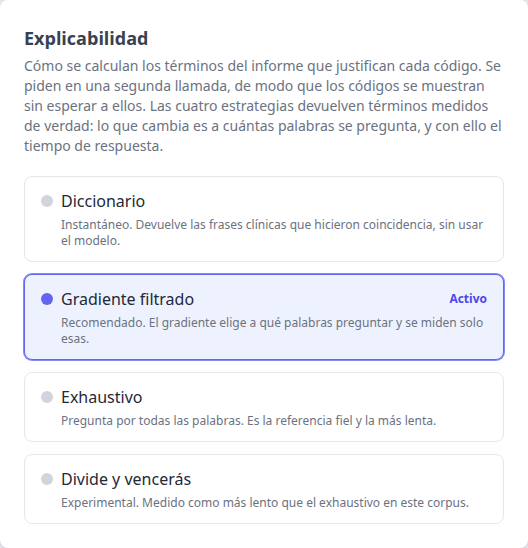
\includegraphics[width=0.6\textwidth]{figs/ui-admin-explicabilidad}
\caption{\emph{Backoffice} de administración: selección de la estrategia de atribución de términos (diccionario, gradiente filtrado, exhaustivo o divide y vencerás). Está activo el gradiente filtrado, que es el que sirve el sistema.}
\label{fig:admin-explicabilidad}
\end{figure}

\paragraph{El diccionario como explicación inmediata.}
Queda una cuarta vía que no consume el \emph{encoder} en absoluto: devolver las frases clínicas que hicieron coincidencia por expresión regular. Responde en 0{,}58~s, ochenta y tres veces más rápido que el método exhaustivo, y en el motor fusionado esos términos ya están calculados cuando se responde a la predicción, porque la coincidencia se ejecutó para ordenar los códigos.

Sus dos límites también están medidos. Cubre el 63~\% de los códigos propuestos: cuando el bloque no ha hecho coincidencia, ese código se queda sin justificación léxica. Y solo el 15~\% de las palabras que el modelo considera importantes aparece dentro de las frases que encuentra el diccionario, de modo que ambas fuentes señalan evidencias distintas en el 85~\% de los casos.

Esa última cifra es la que justifica mostrar las dos y no elegir una. Si coincidieran, bastaría con la barata; al ser mayoritariamente complementarias, cada una aporta información que la otra no tiene, y el codificador clínico dispone de dos justificaciones independientes de la misma propuesta. Conviene subrayar que no compiten en la misma tarea: el diccionario explica por qué el informe apunta a ese bloque, con frases literales, y el modelo explica qué palabras sostienen el código concreto dentro del bloque. Compararlas con la misma métrica produciría un número bajo que se leería como que el diccionario explica peor, cuando lo que hace es explicar otra cosa.

\paragraph{Clasificador de diccionario.}
Para el motor basado en reglas, la explicabilidad es directa e inherente al diseño: el clasificador devuelve los términos clínicos concretos del informe que activaron cada código (\texttt{matched\_terms}), extraídos mediante las expresiones regulares construidas con spaCy. Estos términos se presentan al usuario de la misma forma que los triggers del motor BERT.

\paragraph{Representación visual.}
Los términos de cada código se presentan como \emph{chips} bajo su descripción, y el color distingue su procedencia: los que provienen del diccionario son coincidencias literales del informe y los del modelo son las palabras cuya eliminación más reduce el \emph{logit}. Son evidencias de distinta naturaleza, así que la interfaz las etiqueta en lugar de fundirlas en una única lista ordenada, y una nota emergente explica de dónde sale cada una. Cuando las palabras del modelo aún se están calculando, la tarjeta muestra los términos léxicos que ya tiene junto a un indicador de progreso, en lugar de dejar el espacio vacío.

\paragraph{Trabajo futuro.}
Una extensión natural es la estimación de intervalos de confianza en las atribuciones mediante múltiples perturbaciones con ruido (\emph{SmoothGrad}~\cite{Smilkov17}), o el uso de \emph{SHAP KernelExplainer}~\cite{Lundberg17} para obtener valores de Shapley con garantías de equidad en la distribución de la importancia entre palabras. Ambos métodos añaden coste computacional pero proporcionan propiedades teóricas más sólidas.

\subsection{Autenticación y seguridad}
\label{sec:seguridad}

El sistema implementa autenticación mediante registro con confirmación por email. Al registrarse, el usuario recibe un email con un enlace de confirmación generado con \texttt{Phoenix.Token}. Una vez confirmada la cuenta, el inicio de sesión devuelve un token Bearer que el frontend almacena en \texttt{localStorage} y envía en la cabecera \texttt{Authorization} de cada petición REST y en el \emph{handshake} del WebSocket. El \emph{plug} \texttt{RequireAuth} verifica el token en todas las rutas protegidas. Los tokens tienen una validez de \textbf{una hora} (\texttt{max\_age: 3\_600}); pasado ese tiempo, cualquier petición es rechazada con un error 401, lo que limita la ventana de exposición ante un robo de sesión. La Figura~\ref{fig:auth-flujo} resume el flujo de autenticación completo.

\begin{figure}[ht]
\centering
\resizebox{0.9\textwidth}{!}{
\begin{tikzpicture}[
  every node/.style={font=\small\sffamily},
  paso/.style={draw=aquaESI!80, fill=aquaESI!12, thick, rectangle, rounded corners=3pt,
              minimum width=10.5cm, minimum height=0.95cm, align=center},
  mail/.style={draw=ocre!80, fill=ocre!15, thick, rectangle, rounded corners=3pt,
               minimum width=10.5cm, minimum height=0.95cm, align=center},
  chk/.style={draw=turquesa!80, fill=turquesa!15, thick, rectangle, rounded corners=3pt,
              minimum width=10.5cm, minimum height=0.95cm, align=center},
  arr/.style={->, >=Stealth, thick},
  node distance=0.55cm,
]
\node[paso] (reg) {1. Registro: \texttt{POST /auth/register} (contraseña con \emph{hash} bcrypt)};
\node[mail, below=of reg] (mail) {2. Correo de confirmación con enlace firmado (\texttt{Phoenix.Token})};
\node[paso, below=of mail] (conf) {3. Confirmación: \texttt{GET /auth/confirm/:token} $\rightarrow$ cuenta activada};
\node[paso, below=of conf] (login) {4. Inicio de sesión: \texttt{POST /auth/login} $\rightarrow$ \{user, token Bearer\} (validez 1\,h)};
\node[paso, below=of login] (use) {5. Peticiones autenticadas: \texttt{Authorization: Bearer} en REST y en el \emph{handshake} WebSocket};
\node[chk, below=of use] (auth) {6. \texttt{RequireAuth} verifica el token (\texttt{Phoenix.Token.verify}, \texttt{max\_age=3600}); si no, HTTP 401};

\draw[arr] (reg) -- (mail);
\draw[arr] (mail) -- (conf);
\draw[arr] (conf) -- (login);
\draw[arr] (login) -- (use);
\draw[arr] (use) -- (auth);
\end{tikzpicture}
}
\caption{Flujo de autenticación: del registro con confirmación por correo a la verificación del token \emph{Bearer} (\texttt{Phoenix.Token}, validez de una hora) en cada petición REST y en el \emph{handshake} del WebSocket.}
\label{fig:auth-flujo}
\end{figure}

Las contraseñas se almacenan hasheadas con bcrypt y se exige una longitud mínima de \textbf{12 caracteres} para reducir la vulnerabilidad ante ataques de fuerza bruta. El servicio de email se implementa con Swoosh y, en el entorno de desarrollo, se captura con Mailpit (accesible en \texttt{http://localhost:8025}).

La política CORS del backend se gestiona mediante el \emph{plug} \texttt{CORSPlug} en el \emph{endpoint} Phoenix. Los orígenes permitidos se leen en tiempo de ejecución desde la variable de entorno \texttt{CORS\_ORIGINS}, lo que permite restringir el acceso a los dominios exactos del frontend sin modificar el código. Los métodos permitidos son \texttt{GET}, \texttt{POST}, \texttt{PUT}, \texttt{DELETE} y \texttt{OPTIONS}; las cabeceras autorizadas son \texttt{Authorization}, \texttt{Content-Type} y \texttt{Accept}. En producción, \texttt{CORS\_ORIGINS} se establece al dominio \texttt{clicoder.app}, de modo que cualquier petición cruzada desde un origen distinto es rechazada antes de llegar a la lógica de la aplicación.

\subsubsection{Limitación de peticiones (\emph{rate limiting})}

Los \emph{endpoints} de autenticación (\texttt{POST /auth/register}, \texttt{POST /auth/login} y \texttt{GET /auth/confirm/:token}) están protegidos por un mecanismo de limitación de peticiones implementado mediante una tabla ETS (\emph{Erlang Term Storage}) local, sin dependencias externas. El \emph{plug} \texttt{AppWeb.Plugs.RateLimit} mantiene una ventana deslizante de 60 segundos por dirección IP: si la misma IP supera las 10 peticiones en ese intervalo, el servidor responde con el código HTTP 429 (\emph{Too Many Requests}) antes de ejecutar cualquier lógica de negocio. Este límite dificulta los ataques de fuerza bruta sobre el formulario de inicio de sesión sin necesitar infraestructura adicional.

\subsubsection{Cabeceras de seguridad HTTP}

El \emph{endpoint} Phoenix incluye el \emph{plug} \texttt{put\_security\_headers}, que añade a todas las respuestas un conjunto de cabeceras defensivas:

\begin{itemize}
 \item \texttt{X-Frame-Options: DENY} impide que la aplicación sea embebida en un \texttt{<iframe>}, previniendo ataques de \emph{clickjacking}.
 \item \texttt{X-Content-Type-Options: nosniff} fuerza al navegador a respetar el tipo MIME declarado, evitando la ejecución involuntaria de recursos mal tipificados.
 \item \texttt{Referrer-Policy: strict-origin-when-cross-origin} limita la información del \emph{referer} enviada en peticiones cruzadas, reduciendo la filtración de URLs internas.
 \item \texttt{Strict-Transport-Security: max-age=31536000; includeSubDomains} (HSTS) obliga al navegador a usar HTTPS durante un año para el dominio y todos sus subdominios, eliminando la posibilidad de ataques de degradación de protocolo (\emph{SSL stripping}).
\end{itemize}

\subsubsection{Auditoría de dependencias}

Un sistema que trata datos de salud hereda las vulnerabilidades de todo lo que importa, no solo las de su propio código, así que las tres bases de código se auditan por separado: \texttt{make audit-backend} (\texttt{mix hex.audit} sobre Elixir), \texttt{make audit-js} (\texttt{npm audit} sobre el frontend) y \texttt{make audit-python} (\texttt{pip-audit} sobre el motor de IA), agrupados bajo \texttt{make audit}. Elixir no tiene paquetes retirados ni vulnerables. El frontend partía de diecisiete avisos; \texttt{npm audit fix} resolvió catorce sin subir ninguna dependencia de versión mayor, y las tres restantes están en \texttt{@vitest/mocker}, herramienta de pruebas que no llega al navegador y para la que no hay parche publicado todavía. El motor de IA tiene un aviso sin arreglo publicado en \texttt{diskcache} (\texttt{PYSEC-2026-2447\allowbreak}): deserializa con \texttt{pickle} por defecto, lo que permite ejecución de código si un atacante consigue escritura en el directorio de caché. Es dependencia transitiva de \texttt{llama\_cpp\_python} (el motor del resumidor LLM, sección~\ref{sec:resumidor}), pero solo a través de la clase \texttt{LlamaDiskCache}, que ningún módulo propio instancia: el resumidor usa la caché en memoria por defecto de la biblioteca, de modo que el código que ejercitaría la vulnerabilidad no llega a ejecutarse aunque el resumidor esté activo.

\subsection{Observabilidad}
\label{sec:observabilidad}

Un prototipo desplegado y en uso necesita responder a dos preguntas distintas: si algo se ha roto, y si el sistema se está comportando como se espera. Se resuelven con dos mecanismos separados.

\textbf{Seguimiento de errores con Sentry}. El backend y el motor de IA envían sus excepciones no controladas a Sentry, cada uno con su propio DSN (\texttt{SENTRY\_DSN} y \texttt{SENTRY\_DSN\_AI}), de modo que un fallo del servicio de inferencia no se confunde con uno de la capa de aplicación. En Elixir la integración se registra en el \emph{endpoint} de Phoenix y captura además los errores de los procesos supervisados, que de otro modo se perderían en el reinicio del árbol de supervisión. En Python las excepciones de las peticiones se capturan con las integraciones de FastAPI y Starlette, y los fallos de carga del modelo se notifican explícitamente con \texttt{sentry\_sdk.capture\_exception}, porque un arranque degradado no lanza ninguna excepción hacia el cliente y pasaría inadvertido. Lo que importa aquí no es tener la herramienta, sino que un error en producción llega con el rastro de pila y el contexto de la petición sin depender de que alguien mire los registros: ese contexto es también lo que obliga al filtrado descrito a continuación.

\textbf{Métricas con Prometheus y Grafana}. El motor de IA expone \texttt{GET /metrics} con la latencia de inferencia por motor y el estado de carga de cada modelo; el backend publica las suyas en el puerto 9568. Prometheus las recoge junto a las del anfitrión, los contenedores y el proxy, y una sonda \emph{blackbox} comprueba desde fuera que los tres servicios responden. Grafana los presenta en paneles aprovisionados desde el repositorio (Anexo~\ref{cap:AnexoK}). La distinción con Sentry es deliberada: Sentry dice qué ha fallado, las métricas dicen si está fallando algo que todavía nadie ha notado.

\subsubsection{Filtrado de datos sensibles en el sistema de monitorización}

Un aviso de error viaja a un servicio de terceros, de modo que todo lo que se adjunte al aviso sale del sistema. Eso convierte a la monitorización en el punto por el que los datos pueden escaparse sin que nadie lo note, porque el sistema sigue funcionando igual mientras filtra. El criterio adoptado es que hacia fuera solo salgan \textbf{identificadores}, nunca contenido: con el identificador de la conversación y el del usuario, el error se investiga consultando la base de datos local; el informe clínico, el correo y la dirección IP no aportan nada para depurar y son precisamente lo que no puede salir.

En el backend, el \emph{callback} \texttt{before\_send} del módulo \texttt{AppWeb.SentryFilter} interviene cada evento antes de enviarlo. Sustituye por \texttt{[FILTERED]} los campos sensibles del cuerpo de la petición, recorriendo también los mapas anidados: \texttt{password}, \texttt{password\_hash}, \texttt{token}, \texttt{content} (texto del informe), \texttt{report\_text}, \texttt{authorization} y \texttt{cookie}. A esos se añaden tres piezas que el filtrado por nombre de campo no cubría:

\begin{itemize}
 \item La \textbf{cadena de consulta} completa, porque por ahí viaja el token de confirmación de correo (\texttt{GET /auth/confirm/:token}), que da acceso a la cuenta.
 \item La \textbf{dirección IP} del cliente, tanto en \texttt{REMOTE\_ADDR} como en las cabeceras \texttt{X-Forwarded-For} y \texttt{X-Real-IP}. Es dato personal del artículo~4 del RGPD.
 \item Los \textbf{datos del usuario} adjuntos al evento, de los que solo se conserva el identificador de la base de datos.
\end{itemize}

En el motor de inteligencia artificial el riesgo era mayor y de otra naturaleza, porque este servicio recibe el informe clínico en el cuerpo de cada petición. El SDK de Python adjunta por omisión \textbf{las variables locales de cada marco de la pila}, de modo que una excepción durante una predicción habría enviado el texto del informe íntegro: la variable que lo contiene es un argumento de la función que estaba ejecutándose. Se desactiva explícitamente con \texttt{include\_local\_variables}, junto a \texttt{send\_default\_pii} y \texttt{max\_request\_body\_size}, que impiden respectivamente el envío de datos identificativos y del cuerpo de la petición.

Este filtrado no es una capa opcional de endurecimiento sino parte del cumplimiento descrito en la sección~\ref{sec:rgpd}, de modo que se fija con pruebas (\texttt{backend/test/app\_web/sentry\_filter\_test.exs}): comprueban que el informe no sale ni anidado, que la IP y la cadena de consulta desaparecen, y que del usuario solo queda el identificador. Escribirlas obligó a que la dependencia de Sentry estuviera disponible también en el entorno de pruebas, porque hasta entonces el módulo que protege los datos clínicos era el único que no podía ejecutarse en la batería. Al hacerlo apareció además un fallo que no era de privacidad sino de robustez: el filtro lanzaba una excepción cuando el evento llegaba sin cabeceras, y un filtro que falla no envía el aviso, con lo que el error original se perdía.

\subsection{Conformidad con el Reglamento General de Protección de Datos (RGPD)}
\label{sec:rgpd}

El Reglamento (UE) 2016/679, conocido como RGPD~\cite{RGPD16}, establece el marco jurídico de referencia para el tratamiento de datos personales en la Unión Europea. Su aplicación es especialmente relevante en sistemas sanitarios, donde se procesan categorías especiales de datos (artículo~9 RGPD): los informes clínicos introducidos por el usuario y los diagnósticos CIE-10 inferidos constituyen datos relativos a la salud y, por tanto, están sujetos al régimen de protección reforzada.

El sistema maneja tres categorías de datos: (1)~\textbf{datos identificativos} del usuario (nombre, apellidos, nombre de usuario y dirección de correo electrónico); (2)~\textbf{datos de autenticación} (contraseña hasheada con bcrypt y token de sesión); y (3)~\textbf{datos clínicos} (texto libre de informes médicos y los códigos CIE-10 asociados). El diseño técnico incorpora medidas organizativas y de ingeniería orientadas a cumplir los principios del artículo~5 RGPD (licitud, lealtad y transparencia; limitación de la finalidad; minimización de datos; exactitud; limitación del plazo de conservación; integridad y confidencialidad), así como los derechos reconocidos en los artículos~17 y~20~\cite{RGPD16}.

\subsubsection{Artículo 5, Principios relativos al tratamiento}

\begin{itemize}
 \item \textbf{Minimización de datos}: el sistema solicita únicamente los datos imprescindibles para el registro (nombre, apellidos, nombre de usuario, correo y contraseña). El perfil no incluye número de teléfono, fecha de nacimiento ni ningún otro dato opcional. Los informes clínicos se tratan exclusivamente para generar la propuesta de codificación y no se comparten con terceros.
 \item \textbf{Integridad y confidencialidad}: las contraseñas se almacenan exclusivamente como \emph{hash} bcrypt; ningún proceso del sistema accede al valor en claro. Las comunicaciones se cifran en tránsito mediante TLS (forzado mediante HSTS), y el token de sesión expira a la hora de ser emitido. Los datos sensibles se redactan antes de enviarse al sistema de monitorización externo Sentry (véase sección~\ref{sec:seguridad}).
 \item \textbf{Limitación del plazo de conservación}: el usuario puede eliminar sus datos en cualquier momento, tanto a nivel de conversación individual como de cuenta completa, sin necesidad de contactar con el responsable del tratamiento.
\end{itemize}

\subsubsection{Artículo 17, Derecho de supresión (\emph{«derecho al olvido»})}

El RGPD exige que el responsable del tratamiento suprima los datos personales sin dilación indebida cuando el interesado lo solicite (artículo~17.1~\cite{RGPD16}). El sistema implementa dos niveles de supresión para dar respuesta a este derecho sin requerir intervención manual del administrador:

\begin{itemize}
 \item \textbf{Borrado permanente de una conversación} (\texttt{DELETE /api/conversations/\allowbreak{}:id/purge}): elimina de forma irreversible la conversación y todos los datos asociados (mensajes, tarjetas de análisis, códigos predichos y sugerencias de código) mediante una transacción atómica que recorre todas las tablas dependientes en orden inverso a sus claves foráneas antes de eliminar el registro raíz. A diferencia del borrado lógico habitual (que establece \texttt{deleted\_at} y mantiene los datos en base de datos), este \emph{endpoint} busca que no quede rastro en el modelo de lectura. El \emph{endpoint} verifica que la conversación pertenece al usuario autenticado antes de proceder, impidiendo el borrado de datos ajenos.

\paragraph{El conflicto entre \emph{event sourcing} y el derecho de supresión.}
Borrar el modelo de lectura no basta por sí solo, y conviene explicar por qué. El registro de eventos es inmutable por diseño: es la garantía que justifica haber elegido CQRS, porque permite reconstruir cualquier estado pasado y auditar quién hizo qué. Esa misma propiedad choca de frente con el artículo~17: lo que entra en el registro no se puede borrar, de modo que almacenar allí el informe clínico haría imposible atender una solicitud de supresión por mucho que se vaciaran las tablas de lectura.

La solución adoptada es separar el hecho del contenido. Los eventos \texttt{MessageSent} y \texttt{AnalysisRequested} \textbf{no llevan el texto del informe}: registran quién escribió, cuándo y en qué conversación, que es lo que la trazabilidad necesita. El texto se escribe directamente sobre la proyección, que es la tabla que el purgado elimina. La contrapartida, que hay que declarar, es que reproducir el registro de eventos ya no reconstruye el contenido de los mensajes: la auditoría conserva la secuencia de acciones, no el dato de salud. Es una renuncia deliberada, y en un sistema que maneja categorías especiales del artículo~9 el derecho de supresión pesa más que la reconstruibilidad total.

La frontera está fijada con pruebas automáticas (\texttt{App.RgpdEventStoreTest}) que fallan si alguien vuelve a añadir el texto a un evento. Sin ellas el error sería invisible: el sistema seguiría funcionando con normalidad y el informe quedaría almacenado para siempre.

 \item \textbf{Eliminación completa de la cuenta} (\texttt{DELETE /api/users/account}): suprime la totalidad de los datos del usuario en una única transacción de base de datos: primero obtiene los identificadores de todas las conversaciones del usuario (incluidas las que están en la papelera), después elimina en cascada sus dependencias (sugerencias de código, códigos predichos, tarjetas de análisis y mensajes) y finalmente suprime el registro del usuario. Tras el borrado, el token Bearer del usuario queda invalidado de facto, pues el \emph{plug} \texttt{RequireAuth} no puede resolver el sujeto en base de datos.
\end{itemize}

Desde el frontend, el usuario accede a la función de eliminación de cuenta a través del icono \texttt{UserX} situado en la barra lateral. Al pulsarlo se muestra un modal de confirmación con texto explícito sobre la irreversibilidad de la acción y dos botones: cancelar y confirmar. Solo al confirmar se envía la petición \texttt{DELETE}; en caso de éxito, el cliente limpia el estado de sesión y redirige a la pantalla de inicio de sesión.

\subsubsection{Artículo 20, Derecho a la portabilidad de los datos}

El artículo~20 RGPD~\cite{RGPD16} reconoce al interesado el derecho a recibir sus datos en un formato estructurado, de uso común y lectura mecánica, y a transmitirlos a otro responsable del tratamiento sin impedimentos. El \emph{endpoint} \texttt{GET /api/users/export} (autenticado mediante Bearer token) genera y devuelve un archivo JSON que incluye:

\begin{itemize}
 \item El perfil del usuario: nombre, apellidos, nombre de usuario, dirección de correo electrónico y preferencia de idioma.
 \item La totalidad de sus conversaciones, incluyendo conversaciones en la papelera, con sus mensajes completos (contenido y marcas de tiempo) y los códigos CIE-10 predichos con su estado de validación y razonamiento.
 \item La marca de tiempo de generación del fichero.
\end{itemize}

La respuesta se sirve con la cabecera \texttt{Content-Disposition: attachment; filename=\textquotedbl{}datos\_usuario.json\textquotedbl{}} para que el navegador la ofrezca como descarga directa. El fichero resultante es legible por máquina y puede importarse en cualquier sistema que acepte JSON, cumpliendo el requisito de interoperabilidad del artículo~20.2. Desde el frontend, la descarga se activa mediante el icono \texttt{Download} en la barra lateral: el cliente realiza la petición autenticada, convierte la respuesta en un \emph{blob} y lo descarga sin exponer el token en la URL ni abrir una pestaña nueva.

\subsection{Internacionalización}
\label{sec:i18n}

\begin{sloppypar}
La interfaz soporta cinco idiomas: español, inglés, francés, italiano y alemán. Las traducciones del backend se almacenan en ficheros YAML (\texttt{priv/translations/es.yml} y equivalentes) y se sirven a través del \emph{endpoint} \texttt{GET /api/translations/\allowbreak{}:locale}. Conviene declarar su procedencia: solo la versión en español está redactada directamente; \textbf{las otras cuatro se generaron con asistencia de un modelo de lenguaje y no han sido revisadas por hablantes nativos}, de modo que sirven para demostrar que la infraestructura de internacionalización funciona, pero no se presentan como traducciones de calidad profesional. El frontend las carga al arrancar mediante \texttt{I18nContext} y las aplica con la función \texttt{t(key, vars)}, que soporta interpolación de variables. La preferencia de idioma se almacena en la base de datos del usuario y se sincroniza con el backend al cambiar de idioma.
\end{sloppypar}

\subsection{Calidad del código y buenas prácticas}
\label{sec:calidad}

El proyecto aplica un conjunto de principios arquitectónicos y herramientas de calidad de forma consistente en todos sus componentes, lo que permite detectar errores de forma temprana, mantener la coherencia del código y facilitar su evolución a medida que el sistema crece.

\subsubsection{Arquitectura orientada a eventos y CQRS}

Una \textbf{arquitectura orientada a eventos} (\emph{event-driven architecture}, EDA) es un estilo arquitectónico en el que los componentes del sistema se comunican emitiendo y reaccionando a eventos~\cite{Fowler02}. Un evento representa un hecho ocurrido en el pasado, irreversible e inmutable, y no una instrucción dirigida a un destinatario concreto. Los productores de eventos no conocen a sus consumidores; los consumidores se suscriben a los eventos que les interesan y reaccionan de forma independiente. Este desacoplamiento permite que cada componente evolucione, escale y falle de forma autónoma sin afectar al resto del sistema.

\textbf{Event Sourcing}~\cite{Young10} lleva este principio al nivel del modelo de datos: en lugar de almacenar únicamente el estado actual de una entidad (la fila actual en una tabla relacional), el sistema persiste la secuencia completa de eventos que han producido ese estado. El estado actual se obtiene siempre reproduciendo los eventos desde el origen. Esta estrategia proporciona un historial de auditoría completo y gratuito, especialmente relevante en un contexto clínico donde la trazabilidad de las decisiones es un requisito regulatorio, y permite reconstruir el estado del sistema en cualquier instante del pasado.

El patrón \textbf{CQRS}~\cite{Young10} separa el modelo de escritura del modelo de lectura. Los \textbf{comandos} expresan la intención de cambiar el estado del sistema (\texttt{AnalyzeReport}, \texttt{ValidateCode}…); son procesados por los agregados, que validan las invariantes de negocio y emiten los eventos correspondientes. Las \textbf{consultas} operan sobre modelos de lectura desnormalizados, las proyecciones, optimizados para las necesidades de la interfaz y actualizados de forma asíncrona por los proyectores a medida que llegan los eventos. La combinación CQRS/Event Sourcing ofrece tres ventajas concretas para este proyecto: (1)~trazabilidad completa de cada acción clínica sobre cada análisis; (2)~independencia entre la carga de escritura (predicciones del modelo BERT) y la carga de lectura (consultas del historial por el codificador); y (3)~posibilidad de añadir nuevas proyecciones, por ejemplo, estadísticas de uso o informes de calidad, sin modificar el dominio.

En el backend del proyecto, este patrón se implementa mediante la biblioteca Commanded~\cite{commanded2024} sobre PostgreSQL como \emph{event store}; los comandos de dominio y la decisión de persistencia (ADR-04) se detallan en el diseño del backend (sección~\ref{sec:diseno-backend}).

\subsubsection{Principios SOLID}

Los principios SOLID~\cite{MartinCleanCode08,MartinPPP02} son un conjunto de cinco directrices de diseño orientado a objetos formuladas y sistematizadas por Robert C. Martin (\emph{Uncle Bob}) que buscan producir sistemas con bajo acoplamiento, alta cohesión y facilidad de extensión y mantenimiento. Martin los desarrolla en profundidad en \emph{Clean Code}~\cite{MartinCleanCode08} y en \emph{Agile Software Development}~\cite{MartinPPP02}, y los eleva al nivel arquitectónico en \emph{Clean Architecture}~\cite{MartinCleanArch17}.

\begin{itemize}
 \item \textbf{S: principio de responsabilidad única} (\emph{Single Responsibility Principle}, SRP): \emph{«Una clase debe tener una, y solo una, razón para cambiar»}~\cite{MartinPPP02}. En el backend, este principio separa los agregados (lógica de negocio y validación de invariantes), los proyectores (actualización de vistas de lectura) y los manejadores de proceso (\emph{process managers}): cada módulo tiene un único motivo de cambio, de modo que una modificación en las reglas de negocio no obliga a modificar la capa de persistencia ni viceversa.

 \item \textbf{O: principio abierto/cerrado} (\emph{Open/Closed Principle}, OCP): \emph{«Las entidades software deben estar abiertas a la extensión pero cerradas a la modificación»}~\cite{MartinPPP02}. En el motor de IA, la clase \texttt{CIE10Classifier} encapsula la lógica de inferencia de modo que añadir soporte para un nuevo modelo base, una nueva estrategia de umbral o un nuevo formato de salida no requiere modificar el código de inferencia existente, sino extender la clase o intercambiar el artefacto del modelo.

 \item \textbf{L: principio de sustitución de Liskov} (\emph{Liskov Substitution Principle}, LSP): \emph{«Los subtipos deben poder sustituirse por sus tipos base»}~\cite{Liskov87,MartinPPP02}. En el backend, los diferentes adaptadores de Commanded (\texttt{EventStore.Adapters.Postgres}, un eventual adaptador Kafka) implementan la misma interfaz del \emph{event store}; el resto del dominio los usa de forma intercambiable sin necesidad de conocer la implementación concreta.

 \item \textbf{I: principio de segregación de interfaces} (\emph{Interface Segregation Principle}, ISP): \emph{«Los clientes no deben ser forzados a depender de interfaces que no utilizan»}~\cite{MartinPPP02}. En el frontend, los contextos de React están segregados por dominio: \texttt{AuthContext} expone únicamente operaciones de sesión, \texttt{ConversationContext} las del análisis activo e \texttt{I18nContext} las de internacionalización. Ningún componente de la interfaz depende de estado o métodos que no le conciernen, lo que simplifica las pruebas y limita la propagación de re-renderizados.

 \item \textbf{D: principio de inversión de dependencias} (\emph{Dependency Inversion Principle}, DIP): \emph{«Los módulos de alto nivel no deben depender de los módulos de bajo nivel; ambos deben depender de abstracciones»}~\cite{MartinPPP02}. Este principio es el más visible en la arquitectura del backend: el dominio de negocio depende de la abstracción \texttt{EventStore} definida por Commanded, no del adaptador PostgreSQL que la implementa. Sustituir ese adaptador se reduce a cambiar la configuración del supervisor OTP sin modificar ningún agregado, proyector ni manejador de eventos.
\end{itemize}

La aplicación sistemática de estos principios produce sistemas donde cada cambio tiene un alcance acotado y predecible, reduciendo el riesgo de regresiones y facilitando la incorporación de nuevas funcionalidades sin reescribir código existente. Martin sintetiza esta idea en \emph{Clean Code} con la regla de los \emph{boy scouts}~\cite{MartinCleanCode08}: \emph{«Deja el código más limpio de lo que lo encontraste»}, principio que también ha guiado las sesiones de refactorización durante el desarrollo del proyecto.

\subsubsection{Linters, formatters y análisis estático}

Cada componente cuenta con herramientas de formato, linting y análisis estático, integradas como objetivos del \texttt{Makefile}. La ejecución de cada target produce un informe legible en la salida estándar que identifica exactamente el fichero, la línea y la regla infringida, lo que permite corregir los problemas sin abandonar el terminal.

\begin{itemize}
 \item \textbf{Backend (Elixir).}
 \begin{itemize}
 \item \texttt{mix format} / \texttt{mix format --check-formatted}: formateador oficial del lenguaje. En modo \texttt{--check-formatted} falla la compilación si algún fichero no está formateado, lo que asegura la consistencia sin discusión (\texttt{make backend-format}, \texttt{make backend-lint}).
 \item Credo~\cite{Credo} (\texttt{--strict}): analizador estático que detecta antipatrones, módulos con múltiples responsabilidades, código duplicado, complejidad ciclomática elevada y violaciones de estilo. Genera un informe priorizado por categoría (\texttt{make backend-lint}).
 \item Dialyxir~\cite{Dialyxir}: envoltorio de Dialyzer, la herramienta de análisis de tipos de la plataforma Erlang/OTP. Infiere los tipos de las funciones y detecta llamadas imposibles, cláusulas inalcanzables y contratos de tipo rotos sin necesidad de anotaciones explícitas, gracias al análisis de flujo sobre el bytecode BEAM. Genera su informe con \texttt{make backend-dialyzer}.
 \end{itemize}
 \item \textbf{Motor de IA (Python).} Ruff~\cite{Ruff} integra en una única herramienta las capacidades de Flake8, isort y pycodestyle. Comprueba conformidad con PEP\,8, ordenación de importaciones, variables no utilizadas y más de 800 reglas adicionales. Su salida identifica regla, fichero y línea; puede aplicar correcciones automáticas con \texttt{--fix}. Se ejecuta con \texttt{make ai-lint}.
 \item \textbf{Frontend (TypeScript/Next.js).}
 \begin{itemize}
 \item ESLint con \texttt{eslint-config-next}: aplica las reglas recomendadas para React y Next.js, detectando accesibilidad básica, uso incorrecto de hooks y patrones desaconsejados (\texttt{make frontend-lint}).
 \item Compilador TypeScript en modo estricto (\texttt{strict: true}): actúa como analizador estático de tipos en tiempo de compilación. Detecta tipos \texttt{unknown} sin acotar, propiedades inexistentes, asignaciones incompatibles y rutas de código no controladas. Los errores de tipo bloquean la construcción del artefacto de producción (\texttt{next build}).
 \end{itemize}
\end{itemize}

\subsubsection{Cobertura de pruebas}

La cobertura de código se mide de forma independiente en cada componente:

\begin{itemize}
 \item \textbf{Backend:} la herramienta \texttt{mix coveralls} genera informes HTML en \texttt{backend/cover/} que detallan las líneas cubiertas por la suite ExUnit. La cobertura global de líneas es del 92,9\,\%; la sección~\ref{sec:pruebas-backend} detalla la cobertura por módulo y los módulos que quedan sin cubrir.
 \item \textbf{Frontend:} Vitest con el proveedor \texttt{@vitest/coverage-v8} genera los informes al ejecutar \texttt{make frontend-coverage}. V8 instrumenta el código JavaScript directamente a nivel de motor, obteniendo métricas más precisas que los instrumentadores basados en transformaciones de AST.
\end{itemize}

\subsubsection{Docker como plataforma de desarrollo reproducible}

Todo el ciclo de vida del proyecto (desarrollo, pruebas, entrenamiento y despliegue) se orquesta con Docker Compose. Esta decisión tiene dos consecuencias directas para la calidad del proyecto. Primera, el entorno es reproducible: cualquier colaborador puede levantar el sistema completo con \texttt{make up} sin instalar dependencias locales ni configurar versiones de lenguaje. Segunda, los linters y formatters se ejecutan dentro del mismo contenedor que el código de producción (\texttt{make backend-lint}, \texttt{make ai-lint}, \texttt{make frontend-lint}), eliminando las diferencias entre el entorno de desarrollo local y el de CI. Las variantes \texttt{docker-compose.gpu.yml} y \texttt{docker-compose.cpu.yml} permiten ajustar la configuración del motor de IA a la infraestructura disponible sin modificar el resto del sistema.

\section{Pruebas del sistema}

\subsection{Estrategia}

La estrategia de pruebas cubre los tres componentes principales del sistema: el motor de IA, el backend y el frontend. Se distinguen pruebas unitarias, de integración y de sistema, con distinto alcance en cada componente según su naturaleza.

\subsection{Pruebas del motor de inteligencia artificial}

Las pruebas del motor de IA se realizan en dos niveles. A nivel de \emph{baseline}, el clasificador de diccionario se evalúa automáticamente con precisión, \emph{recall}, F1 (micro y macro) y MAP por documento sobre los conjuntos de entrenamiento, validación y prueba de CodiEsp (\texttt{baseline\_dict.py}). A nivel del modelo BERT, las métricas de evaluación (precisión, \emph{recall} y F1-micro y F1-macro) se calculan automáticamente al final de cada época de entrenamiento sobre el conjunto de validación, y al finalizar el entrenamiento se genera una curva de aprendizaje que permite detectar sobreajuste o convergencia prematura.

\subsection{Pruebas del backend}
\label{sec:pruebas-backend}

El backend incluye una suite de 316~pruebas ExUnit organizada en \texttt{backend/test/}, ejecutadas con \texttt{make backend-test}. La cobertura se mide por separado en cada uno de los tres proyectos (Tabla~\ref{tab:cobertura}), porque son bases de código independientes con herramientas y naturaleza distintas, y promediarlas no significaría nada. A ellos se añade una cuarta suite, de extremo a extremo, que no aporta cobertura de línea porque no mide líneas sino recorridos.

\begin{table}[H]
\centering
\small
\caption{Cobertura de línea por proyecto. Generada con \texttt{make backend-coverage}, \texttt{make ai-coverage} y \texttt{make frontend-coverage} (\texttt{make coverage} los ejecuta juntos).}
\label{tab:cobertura}
\begin{tabular}{llrr}
\hline
\textbf{Proyecto} & \textbf{Herramienta} & \textbf{Pruebas} & \textbf{Cobertura} \\
\hline
Backend (Elixir) & \texttt{excoveralls} & 316 & 92{,}9\,\% \\
Motor de IA (Python) & \texttt{pytest-cov} & 383 & 91{,}0\,\%$^{*}$ \\
Frontend (TypeScript) & \texttt{vitest} + \texttt{v8} & 217 & \textbf{98{,}9\,\%}$^{\dagger}$ \\
Extremo a extremo & \texttt{playwright} + \texttt{pytest} & 11 & n/a$^{\ddagger}$ \\
\hline
\end{tabular}

\vspace{2mm}
{\footnotesize $^{*}$ Sobre los seis módulos que se despliegan (\texttt{main}, \texttt{classifier}, \texttt{baseline\_dict}, \texttt{summarizer}, \texttt{rerank\_map}, \texttt{compare\_runs}). Los guiones de entrenamiento y de figuras quedan fuera del cálculo. $^{\dagger}$ Quedan fuera las rutas de Next.js, los primitivos de interfaz generados y los dos módulos que se sustituyen por dobles en todas las pruebas. $^{\ddagger}$ No procede: recorre la aplicación por el navegador y atraviesa los tres proyectos a la vez, de modo que no se puede atribuir su cobertura a ninguno.}
\end{table}

Las tres cifras de cobertura se acercan al 90\,\% pero no significan lo mismo, y conviene decir qué mide cada una. El backend es código de orquestación cuyo comportamiento depende de la interacción entre piezas: las pruebas cubren el agregado, el proyector que materializa el registro de eventos, los canales, los controladores, el panel de administración y los endpoints de protección de datos. En el motor de IA solo se miden los módulos que se despliegan, porque los guiones de entrenamiento y de figuras se ejecutan a mano una vez y se verifican contra los artefactos que producen; contarlos diluiría la cifra sin decir nada del servicio. Dentro de lo medido, lo único que queda descubierto es la función \texttt{main()} de la construcción del diccionario, 328 líneas que encadenan cargadores ya probados por separado. El frontend es el más alto de los tres porque es donde menos código hay y donde el comportamiento se puede ejercitar entero desde el DOM.

Dos observaciones sobre el propio proceso de medir. La primera es que alcanzar esa cobertura exigió antes hacer testable lo que no lo era: faltaba la dependencia que Phoenix necesita para inspeccionar una vista en vivo, sin la cual el panel de administración era imposible de probar, y las llamadas al motor de IA no admitían inyectar el transporte, de modo que su integración no podía ejercitarse sin una red. La segunda es que un objetivo de cobertura invita a maquillar la cifra excluyendo del cálculo lo que no está probado; las exclusiones de cada proyecto se declaran al pie de la Tabla~\ref{tab:cobertura} en lugar de dejarlas en los ficheros de configuración. Las pruebas se distribuyen en cuatro niveles, siguiendo la estructura del código de producción.

\subsubsection*{Pruebas unitarias de dominio}

Las pruebas de la capa de dominio validan las reglas de negocio en aislamiento, sin acceso a la base de datos ni a servicios externos. El módulo \texttt{App.Aggregates.ConversationTest} verifica cada comando (\texttt{StartConversation}, \texttt{SendMessage}, \texttt{AnalyzeReport}, \texttt{ValidateCode}, \texttt{RejectCode}) contra el agregado, comprobando tanto los caminos felices (emisión del evento esperado) como los caminos de error (intento de validar un código ya validado, análisis con otro pendiente, etc.). El módulo \texttt{App.AIEngineSettingsTest} cubre el agente OTP de configuración del motor de inferencia, verificando el valor por defecto, las transiciones válidas entre motores (\texttt{bert}/\texttt{dict}/\texttt{both}) y el rechazo de valores fuera del conjunto permitido.

\subsubsection*{Pruebas de integración con la base de datos}

Las pruebas de integración usan el adaptador de sandbox de Ecto (\texttt{Ecto.\allowbreak{}Adapters.\allowbreak{}SQL.\allowbreak{}Sandbox}) para ejecutar cada test dentro de una transacción que se revierte automáticamente al finalizar, manteniendo el aislamiento entre tests. Este nivel cubre:

\begin{itemize}
 \item \textbf{Esquemas de proyección}: \begin{sloppypar}\texttt{App.Projections.ConversationProjectorTest} verifica las operaciones Ecto sobre los cuatro modelos relacionales (\texttt{ConversationProjection}, \texttt{MessageProjection}, \texttt{PredictedCodeProjection}, \texttt{Analys\-isCardProjection}), incluyendo inserciones, actualizaciones de estado (\texttt{pending} $\to$ \texttt{validated}/\texttt{rejected}), borrado suave y ordenación.\end{sloppypar}
 \item \textbf{Cuentas de usuario}: \texttt{App.AccountsTest} comprueba el registro, la confirmación por correo y la autenticación; \texttt{AppWeb.AuthControllerTest} verifica los \emph{endpoints} REST de registro, inicio y cierre de sesión.
 \item \textbf{Plug de autenticación}: \texttt{AppWeb.Plugs.RequireAdminTest} verifica los cuatro ramos de la lógica de autorización (sin sesión, usuario no-admin, usuario admin, identificador inexistente), alcanzando cobertura completa del plug.
\end{itemize}

\subsubsection*{Pruebas de API REST}

Los controladores se prueban mediante solicitudes HTTP reales a través de \texttt{AppWeb.\allowbreak{}ConnCase}. Se cubren los \emph{endpoints} de traducciones de la interfaz (\texttt{/api/translations/\allowbreak{}:locale}), el catálogo CIE-10 (\texttt{/api/cie10/search}, \texttt{/api/cie10/codes/:code}), la gestión de conversaciones y el proxy al motor de IA (\texttt{/api/ai/count-tokens}). Este último incluye tres escenarios: parámetro \texttt{text} ausente (422), valor no textual (422), y motor de IA no disponible (503), situación que siempre se produce en el entorno de test porque el servicio FastAPI no arranca con la suite ExUnit.

\subsubsection*{Pruebas de canal WebSocket}

Los canales Phoenix se prueban con \texttt{Phoenix.ChannelTest}, que simula la conexión WebSocket sin levantar un servidor HTTP real. Las pruebas cubren la autenticación del socket (token válido, ausente e inválido), la unión a conversaciones existentes (carga del historial con mensajes, códigos y tarjetas de análisis) y a conversaciones nuevas (despacho de \texttt{StartConversation} mediante Commanded), y los cinco tipos de mensajes entrantes: \texttt{send\_message}, \texttt{analyze\_report}, \texttt{validate\_code}, \texttt{reject\_code} y \texttt{suggest\_code}.

\subsubsection*{Pruebas de extremo a extremo}

Las anteriores prueban cada proyecto por dentro, con el resto sustituido por dobles. Eso deja fuera precisamente lo que solo falla cuando las piezas se juntan, y por eso hay una cuarta suite que recorre la aplicación por el navegador con Playwright (\texttt{make e2e-tests}, \texttt{e2e/test\_flujos.py}). Son once flujos: el alta y su confirmación, el rechazo de un correo duplicado, el inicio de sesión con credenciales válidas e inválidas, el envío de un informe con recepción de códigos, la validación y el rechazo de un código con motivo, y el borrado de una conversación a la papelera.

La confirmación del correo no se simula. El test lee el mensaje del servidor SMTP de desarrollo por su API y sigue el enlace, de modo que la prueba cubre también el envío. Esa decisión encontró un fallo que llevaba tiempo latente: la variable que indica el servidor de correo no estaba definida en el contenedor del backend, así que la configuración caía al valor por omisión, que dentro del contenedor no escucha, y \textbf{ningún correo de confirmación se había entregado nunca en el entorno de desarrollo}. El sistema no daba error: registraba al usuario y mostraba la pantalla de «revisa tu correo».

\subsubsection*{Lo que queda sin cubrir}

Una versión anterior de este trabajo dejaba fuera de la suite cuatro bloques enteros: la tarea de importación del catálogo, los módulos de configuración OTP, los \emph{structs} de comandos y eventos, y los LiveViews de administración. Los tres primeros se justificaban por falta de lógica propia; el cuarto, por no ser parte del flujo clínico. Al revisar esa decisión resultó que la razón real del cuarto era otra: faltaba en \texttt{mix.exs} la dependencia que \texttt{Phoenix.LiveViewTest} necesita para inspeccionar el HTML renderizado, de modo que no es que no se hubiera priorizado, es que no se podía. Añadida la dependencia, los tres bloques con lógica se cubrieron: la tarea de importación queda en el 92,5\,\% y los LiveViews de administración entre el 86,4\,\% y el 100\,\%. Los \emph{structs} de comandos y eventos aparecen al 100\,\% porque el agregado los construye en cada escenario.

Lo que sigue descubierto son ramas de error que exigirían provocar fallos de infraestructura: el árbol de supervisión (\texttt{App.Application}, 71,4\,\%), la persistencia de la configuración del resumidor, que escribe en una tarea asíncrona sin conexión del \emph{sandbox} (\texttt{App.SummarizerSettings}, 67,3\,\%), y los caminos de reintento del limitador de peticiones. Son los sitios donde una prueba resulta intermitente, y un test que falla una vez de cada diez se acaba ignorando, que es peor que no tenerlo.

\subsection{Pruebas del frontend}

El frontend utiliza Vitest como \emph{framework} de pruebas, con \texttt{@testing-library/react} sobre \texttt{jsdom} para montar componentes sin un navegador real. La configuración se encuentra en \texttt{frontend/\allowbreak vitest.config.ts} y los informes se escriben fuera del árbol del proyecto porque el directorio por defecto quedó en manos de \texttt{root} tras ejecutar el contenedor como superusuario, y \emph{vitest} lo borra al arrancar. Las 217~pruebas se reparten en ocho ficheros: dos contextos concentran la mayoría (\texttt{ConversationContext.test.tsx}, 65~pruebas; \texttt{AuthContext.test.tsx} e \texttt{I18nContext.test.tsx}) y dos componentes cubren la interfaz de análisis (\texttt{ChatInterface.test.tsx}, 45~pruebas; \texttt{ConversationSidebar.test.tsx}).

El punto de diseño que hace testable el frontend es que ninguna prueba abre una conexión real: el módulo \texttt{@/lib/socket} se sustituye por un doble en memoria que expone las mismas funciones \texttt{join}/\texttt{on}/\texttt{push}/\texttt{leave} del cliente de Phoenix, pero sin \emph{socket} de por medio. Los tests capturan el \emph{callback} que la aplicación registra para cada evento y lo invocan directamente con los datos que quieran simular, de modo que \texttt{ConversationContext.test.tsx} ejercita el mismo recorrido descrito en la subsección anterior (recepción de \texttt{analysis\_card\_received} y \texttt{triggers\_received}) sin levantar el backend. Sobre esa base, \texttt{ChatInterface.test.tsx} cubre la validación y el rechazo de un código (exigiendo motivo), la aparición progresiva de las evidencias de un código antes y después de que lleguen los \emph{triggers}, el aviso de longitud máxima de tokens y el atajo de teclado \texttt{Ctrl+Enter}.

\subsection{Pruebas de sistema}

Las pruebas de sistema verifican el flujo completo de uso: registro, inicio de sesión, envío de un informe clínico, recepción de las tarjetas de análisis y validación de códigos. En el entorno de desarrollo se utiliza el motor de IA simulado (\texttt{ai\_engine\_mock}) para desacoplar las pruebas de sistema del proceso de entrenamiento.

\paragraph{Un caso real, de principio a fin.} Tomando el informe de la Figura~\ref{fig:ejemplo-explicabilidad}, el recorrido completo de un análisis es el siguiente: el frontend envía el texto al backend por el canal WebSocket (\texttt{analyze\_report}); el backend lo reenvía a \texttt{POST /predict} del motor de IA, que devuelve entre sus códigos el \texttt{F17.210} (dependencia de nicotina, cigarrillos); el backend persiste el código como \texttt{PredictedCode} pendiente de revisión y emite el evento \texttt{analysis\_card\_received} por \texttt{ConversationChannel}, que la interfaz muestra de inmediato como una tarjeta de códigos. Al desplegar el código, una segunda petición a \texttt{/explain} devuelve los términos que lo justifican (\emph{cigarrillos}, 0,41; \emph{posteriormente}, 0,16; \emph{micciones}, 0,14; \emph{persistente}, 0,12; \emph{normales}, 0,11; los mismos que resalta la Figura~\ref{fig:ejemplo-explicabilidad}) y el codificador clínico valida o rechaza el código con esa evidencia delante.

Conviene precisar qué parte de ese recorrido está comprobada con el modelo real y cuál con el simulado, porque no coinciden. La figura citada sí procede del \emph{checkpoint} de producción: \texttt{ai\_engine/figura\_explicabilidad.py} carga el modelo entrenado y predice sobre un informe real del conjunto de prueba de CodiEsp. La suite automática de pruebas, en cambio, no llega a tocarlo en ningún nivel: los propios tests del motor de IA (\texttt{ai\_engine/tests/test\_api.py}) sustituyen el clasificador por un doble (\texttt{unittest.mock.MagicMock}) para no cargar 600\,M de parámetros en cada ejecución, y las pruebas de sistema y de extremo a extremo corren contra \texttt{ai\_engine\_mock}, un servicio distinto que ni siquiera importa \texttt{classifier.py}. El modelo real solo se ejercita fuera de la suite de tests: durante el propio entrenamiento y evaluación (sección~\ref{sec:entrenamiento} y Anexo~\ref{cap:AnexoH}) y en los guiones de análisis que producen las cifras y figuras de este capítulo (\texttt{bench\_predict.py}, \texttt{bench\_explain.py}, \texttt{error\_analysis.py}, \texttt{figura\_explicabilidad.py}). Es una separación deliberada y no un descuido: medir el modelo es un problema estadístico que se resuelve con F1 y MAP sobre el conjunto de prueba, mientras que las pruebas de software verifican que las piezas se comunican correctamente, algo que un doble barato comprueba igual de bien y mucho más rápido que cargar el \emph{encoder} en cada ejecución.

\section{Despliegue}

\subsection{Arquitectura de despliegue}

El proyecto distingue dos entornos con herramientas de orquestación distintas según sus necesidades.

\textbf{Desarrollo y pruebas.} Cada componente reside en su propio contenedor con su \texttt{Dockerfile} específico, orquestados mediante Docker Compose. La configuración base (\texttt{docker-compose.yml}) define los servicios y sus dependencias; las variantes \texttt{docker-compose.\allowbreak{}gpu.yml} y \texttt{docker-compose.\allowbreak{}cpu.yml} permiten configurar el motor de IA con o sin aceleración por GPU. El Makefile centraliza las operaciones habituales del ciclo de desarrollo: levantar el sistema, aplicar migraciones, lanzar los tests o reconstruir el motor de IA tras un nuevo entrenamiento.

Los servicios y sus puertos de escucha en el entorno local son los que se indican en la tabla~\ref{tab:servicios-puertos}.

\begin{table}[H]
\centering
\caption{Servicios del sistema y puertos de escucha en el entorno local.}
\label{tab:servicios-puertos}
\begin{tabular}{lll}
\hline
\textbf{Servicio} & \textbf{Tecnología} & \textbf{URL local} \\
\hline
Frontend & Next.js 16 & \texttt{http://localhost:3000} \\
Backend & Phoenix 1.8 & \texttt{http://localhost:4000} \\
AI Engine & FastAPI & \texttt{http://localhost:8000} \\
Base de datos & PostgreSQL 18 & \texttt{localhost:5432} \\
Mailpit (email dev) & Mailpit & \texttt{http://localhost:8025} \\
\hline
\end{tabular}
\end{table}

\textbf{Despliegue.} El sistema se sirve desde una estación de trabajo propia, publicada en Internet mediante un túnel de Cloudflare, utilizando el mismo Docker Compose del entorno de desarrollo complementado con Traefik como proxy inverso (véase el Anexo~\ref{cap:AnexoI}). El dominio está protegido por Cloudflare, que actúa como primera línea de defensa frente a bots, \emph{scraping} y ataques de denegación de servicio antes de que el tráfico llegue al servicio. Traefik enruta el tráfico a cada servicio según etiquetas declaradas en los propios contenedores; el certificado TLS público lo genera Cloudflare, de modo que el sistema no gestiona certificados ni usa Let's Encrypt (Anexo~\ref{cap:AnexoI}). El ciclo de despliegue completo se reduce a \texttt{make setup \&\& make deploy GPU=1}. La justificación de coste frente a un servicio en la nube gestionado y la portabilidad de la arquitectura dockerizada se detallan en el Anexo~\ref{cap:AnexoI}.

\subsection{Puesta en marcha}

El sistema se levanta con el comando \texttt{make up} desde la raíz del repositorio, que ejecuta \texttt{docker compose up} con la configuración apropiada. Las migraciones de base de datos se aplican con \texttt{make backend-migrate}. El modelo de IA se entrena con \texttt{make ai-train-gpu}, y el contenedor del motor de IA se reconstruye con \texttt{make build-ai} tras un nuevo entrenamiento.

La imagen base del motor de IA (\texttt{Dockerfile.ml-base}) instala las dependencias Python más pesadas (PyTorch, Transformers) en una capa separada, de modo que las reconstrucciones posteriores, que solo cambian el código de aplicación, son significativamente más rápidas.

\subsection{Configuración de email en producción}

El sistema envía emails transaccionales en dos situaciones: la confirmación de cuenta al registrarse y, en caso de implementarse en el futuro, la recuperación de contraseña. En el entorno de desarrollo este tráfico es capturado por Mailpit. En producción, sin embargo, la entregabilidad de estos mensajes es un requisito funcional crítico: si el email de confirmación no llega al codificador clínico, el flujo de registro queda bloqueado y el usuario no puede acceder al sistema.

Los principales proveedores de correo (Gmail, Outlook, los servidores corporativos hospitalarios) aplican filtros antispam cada vez más estrictos que rechazan o clasifican como sospechosos los mensajes procedentes de dominios sin autenticación correctamente configurada. En un contexto sanitario esto se agrava: los sistemas de filtrado de hospitales y centros de salud suelen tener políticas más restrictivas que el correo de consumo, precisamente para proteger a los profesionales de ataques de \emph{phishing} que suplanten aplicaciones clínicas. Un sistema de codificación que envía emails con tokens de acceso es un objetivo de suplantación especialmente sensible. Por ello, la autenticidad del dominio remitente se respalda mediante tres mecanismos estándar configurados en el DNS:\nopagebreak[4]

\begin{itemize}
 \item \textbf{SPF} (\emph{Sender Policy Framework}): registro TXT en el DNS que declara qué servidores están autorizados a enviar email en nombre del dominio. Impide que terceros suplanten el dominio remitente en la cabecera \texttt{From}.
 \item \textbf{DKIM} (\emph{DomainKeys Identified Mail}): firma criptográfica añadida a cada mensaje por el servidor de envío. El servidor receptor verifica la firma contra la clave pública publicada en el DNS, garantizando que el mensaje no ha sido modificado en tránsito.
 \item \textbf{DMARC} (\emph{Domain-based Message Authentication, Reporting and Conformance}): política que especifica qué debe hacer el servidor receptor cuando un mensaje no supera las comprobaciones SPF o DKIM (ninguna acción, cuarentena o rechazo), y a qué dirección enviar los informes de actividad. Proporciona visibilidad sobre intentos de suplantación del dominio.
\end{itemize}

El proveedor seleccionado para producción es \textbf{Mailjet}, cuyo nivel gratuito permite enviar hasta 200 emails diarios (6.000 mensuales). Dado que la plataforma se encuentra en fase inicial y el volumen de registros es reducido, este límite es suficiente para el tráfico transaccional esperado. Swoosh incluye un adaptador nativo para Mailjet (\texttt{Swoosh.Adapters.Mailjet}) que utiliza la API REST de Mailjet directamente, sin necesidad de relay SMTP: basta con configurar la clave de API y el secreto mediante las variables de entorno \texttt{MAILJET\_API\_KEY} y \texttt{MAILJET\_SECRET\_KEY}. La dirección remitente declarada en \texttt{APP\_HOST} (\texttt{clicoder.app}) debe coincidir con el dominio para el que se han publicado los registros SPF, DKIM y DMARC, de lo contrario los principales proveedores de email clasificarán los mensajes como \emph{spam} o los rechazarán directamente. La arquitectura no requiere ningún cambio para escalar: cuando el volumen de usuarios crezca, basta con contratar un nivel superior en Mailjet y actualizar las variables de entorno, sin modificar ningún componente de la aplicación.

\chapter{Conclusiones}
\label{cap:Conclusiones}

\section{Objetivos alcanzados}

Se ha alcanzado el objetivo principal del trabajo: el diseño e implementación de un prototipo funcional de codificación clínica automática en el estándar CIE-10-ES. El sistema resultante integra un clasificador multilabel basado en \emph{transformers} con una arquitectura completa de software que permite a un codificador clínico enviar casos clínicos en español y recibir propuestas de codificación con una confianza relativa asociada a cada código. La propuesta requiere siempre la revisión completa de un codificador clínico, y los resultados respaldan la viabilidad técnica del enfoque, no su utilidad clínica, que no se ha evaluado con usuarios.

A continuación se revisa el grado de cumplimiento de cada uno de los subobjetivos enumerados en el capítulo~\ref{cap:Objetivo}:

\begin{enumerate}
 \item \textbf{Adquisición y construcción de las fuentes de datos.} Completado. Se descargó el corpus CodiEsp en sus tres particiones (diagnósticos, procedimientos y variante extendida con anotaciones a nivel de \emph{span}), y se desarrollaron los scripts de \emph{scraping} sobre el portal eCIE-maps del Ministerio de Sanidad para obtener el catálogo completo de códigos CIE-10-ES, cuyo formato de descarga pública estructurada no existe. El resultado son los ficheros CSV que alimentan todas las fases posteriores del proyecto. Se implementó el \emph{pipeline} de carga, limpieza y transformación de las anotaciones al formato multilabel requerido por el modelo, incluyendo la conversión de las anotaciones de nivel \emph{span} al nivel de documento empleado en el entrenamiento.


 \item \textbf{Análisis estadístico de las fuentes de datos.} Completado. El análisis de la distribución de longitudes, la frecuencia de aparición de los códigos y el desequilibrio de clases fundamentó las principales decisiones de diseño del modelo: el uso de ponderación de clases en la función de pérdida y la exploración de umbrales de decisión por código, finalmente descartados en favor de un umbral global (véase el subobjetivo siguiente).

 \item \textbf{Módulo clasificador multilabel.} Completado. Tras la comparativa de diez modelos candidatos, cinco evaluados (Anexo~\ref{cap:AnexoA}), se seleccionó \texttt{IIC/RigoBERTa-Clinical} como modelo base y se ajustó mediante \emph{fine-tuning} sobre la partición de diagnósticos de CodiEsp, que es el alcance definido en el capítulo de objetivos; la codificación de procedimientos queda fuera del trabajo. El modelo final, entrenado sobre 500 documentos con 1.767 códigos objetivo, es el clasificador del sistema (umbral global de 0,2 con el clasificador solo y umbral propio sobre la puntuación combinada en el modo fusionado; los umbrales por clase se descartaron por sobreajustar la validación). Sobre el conjunto de prueba alcanza un \textbf{F1-micro de 0,495} y un \textbf{F1-macro de 0,108}, calculados sobre los pares anotados cuyo código pertenece al vocabulario del modelo; sobre todos los pares anotados el F1-micro es 0,444, porque el modelo no puede acertar códigos que no vio en el entrenamiento. La brecha entre F1-micro y F1-macro refleja el fuerte desequilibrio de clases del corpus, donde muchos códigos cuentan con muy pocos ejemplos de entrenamiento.

La calidad del \emph{ranking} de códigos, medida como \textbf{MAP por documento}, es de \textbf{0,454} sobre el \emph{gold} completo con el clasificador solo, directamente comparable con el \emph{benchmark} CodiEsp-D 2020~\cite{miranda2020}. Con el clasificador solo queda en el penúltimo lugar de los diez sistemas comparados, solo por encima de IMS, lo que es coherente con un clasificador plano entrenado con 500 documentos. La cifra de 0,555 corresponde al MAP restringido al vocabulario que el modelo puede predecir y no es comparable con el \emph{benchmark}, cuyos sistemas podían proponer cualquier código.

El \textbf{modo fusionado}, que es el que sirve el sistema por defecto, combina el clasificador con el diccionario de patrones clínicos en un único \emph{ranking} y alcanza \textbf{MAP 0,554 y la segunda posición}, por delante del resto de sistemas, incluidos los diccionarios construidos a mano y los basados en \emph{transformers}, y solo por detrás de IXA-AAA (MAP~0,593). Los resultados sugieren que las dos fuentes de evidencia fallan en sitios distintos: el diccionario acierta el bloque de tres caracteres y no sabe ordenar dentro de él, mientras que el clasificador ordena mejor dentro del bloque pero elige peor el bloque.

 \item \textbf{Backend de gestión y trazabilidad.} Completado. Se desarrolló un backend en Elixir con Phoenix que orquesta el flujo de análisis, gestiona la autenticación con confirmación por correo electrónico y aplica una arquitectura CQRS/\emph{Event Sourcing} sobre PostgreSQL, de modo que cada acción clínica queda registrada como un evento inmutable con su marca temporal y su autoría.

 \item \textbf{Servicio de inferencia (API REST).} Completado. El motor de IA expone mediante FastAPI los \emph{endpoints} de predicción, explicación, resumen y estado (Anexo~\ref{cap:AnexoM}), con una imagen Docker optimizada para PyTorch y soporte para CPU y GPU. El servicio arranca incluso sin modelo entrenado, con un código 503 informativo, lo que facilita el desarrollo y las pruebas.

 \item \textbf{Módulo de generación de resúmenes.} Completado. Se integró un modelo de lenguaje generativo ligero (cuantizado en formato GGUF, ejecutable en CPU) que produce un resumen o una paráfrasis del informe, con modelo, modo y \emph{prompts} configurables desde el \emph{backoffice} y emitido en tiempo real mediante \emph{streaming}. Por tratarse de una ayuda opcional y por su coste computacional, permanece desactivado por defecto en el despliegue y se habilita bajo demanda. Su calidad se validó de forma cualitativa durante el desarrollo; una evaluación cuantitativa sistemática de los resúmenes generados (por ejemplo, con métricas de fidelidad factual y de cobertura de la información clínica) queda pendiente como trabajo futuro.

 \item \textbf{Interfaz web de demostración.} Completada. La interfaz web, desarrollada en Next.js 16 con React 19, permite enviar informes clínicos y visualizar en tiempo real las tarjetas de análisis generadas por el sistema. El codificador puede validar o rechazar individualmente cada código predicho y consultar el historial de análisis anteriores desde el panel lateral.
\end{enumerate}

Más allá de los subobjetivos enumerados, el desarrollo ha incluido componentes complementarios: el \emph{backoffice} de administración, la internacionalización en cinco idiomas, y una infraestructura de despliegue con Docker Compose, Traefik y un túnel de Cloudflare.

\section{Verificación de los requisitos}

La Tabla~\ref{tab:verificacion-req} resume el grado de cumplimiento de los requisitos definidos en la sección~\ref{sec:requisitos} del capítulo~\ref{cap:Desarrollo}.

{\footnotesize
\begin{longtable}{llP{10.4cm}}
\caption{Verificación de los requisitos funcionales (RF) y no funcionales (RNF).}\label{tab:verificacion-req}\\
\hline
\textbf{Req.} & \textbf{Estado} & \textbf{Evidencia} \\
\hline
\endfirsthead
\hline
\textbf{Req.} & \textbf{Estado} & \textbf{Evidencia} \\
\hline
\endhead
RF1 & Cumplido & El motor acepta texto clínico libre sin marcado previo (prueba de \texttt{POST /predict} en \texttt{ai\_engine/\allowbreak{}tests/\allowbreak{}test\_\allowbreak{}api.py}). \\
RF2 & Cumplido & \texttt{POST /predict} devuelve los códigos de diagnóstico predichos (\texttt{test\_\allowbreak{}api.py} y prueba de extremo a extremo de envío de un informe en \texttt{e2e/\allowbreak{}test\_\allowbreak{}flujos.py}). \\
RF3 & Cumplido & Cada código incluye su probabilidad y una confianza relativa normalizada, no calibrada (sección~\ref{sec:confianza-predicciones}); la presencia del campo la comprueba \texttt{test\_\allowbreak{}api.py}. \\
RF4 & No cumplido & El servicio procesa un informe por petición y no existe un \emph{endpoint} que reciba una lista de textos y devuelva los resultados en el mismo orden. Un cliente puede procesar un lote con llamadas independientes a la API (también concurrentes), pero eso no cumple el requisito tal como está formulado. \\
RF5 & Cumplido & API REST documentada con OpenAPI, con \emph{endpoint} de inferencia y de estado (Anexo~\ref{cap:AnexoM}). La especificación la genera FastAPI y no tiene una prueba automática propia; el \emph{endpoint} de estado sí lo cubre \texttt{test\_\allowbreak{}api.py}. \\
RF6 & Cumplido & \texttt{POST /auth/register} da de alta sin conceder acceso y envía un correo con el enlace de \texttt{GET /auth/confirm/:token}; el recorrido completo lo cubre la prueba de extremo a extremo \texttt{test\_confirmar\_el\_correo\_da\_acceso}. \\
RF7 & Cumplido & El canal WebSocket emite \texttt{analysis\_card\_received} con los códigos y, después, \texttt{triggers\_received} con los términos, de modo que la atribución no retrasa la aparición de los códigos (Anexo~\ref{cap:AnexoC}). \\
RF8 & Cumplido & Los eventos \texttt{CodeValidated} y \texttt{CodeRejected} registran la decisión y, en el rechazo, su motivo; la interfaz exige el motivo antes de habilitar la confirmación. \\
RF9 & Cumplido & \texttt{POST /summarize/stream} devuelve el resumen en \emph{streaming} con un modelo cuantizado ejecutable en CPU (prueba del \emph{endpoint} sin modelo en \texttt{test\_\allowbreak{}api.py}; la calidad de los resúmenes no se ha medido). \\
RF10 & Cumplido & Interfaz en Next.js con envío de informes, seguimiento del análisis, términos por código e histórico de análisis con papelera (pruebas de componentes \texttt{Chat\allowbreak{}Interface.\allowbreak{}test.\allowbreak{}tsx} y \texttt{Conversation\allowbreak{}Sidebar.\allowbreak{}test.\allowbreak{}tsx} en \texttt{frontend/\allowbreak{}src/\allowbreak{}test/\allowbreak{}components}). \\
\hline
RNF1 & Cumplido & MAP 0,554 en el modo fusionado servido por defecto (segundo de la comparativa) y 0,454 con el clasificador solo (penúltimo de diez); Tabla~\ref{tab:codiesp-comparativa}. \\
RNF2 & Cumplido & Por informe, en CPU (Ryzen 9 7900X) y en GPU (RTX 4080): predecir 0,331\,s y 0,017\,s; explicar 16,2\,s y 0,51\,s; ciclo completo 16,5\,s y 0,53\,s (Tabla~\ref{tab:latencia}). El requisito acota la predicción, que es lo que el codificador clínico espera para ver los códigos; la explicación se sirve aparte y llega después. \\
RNF3 & Cumplido & Servicios desacoplados en contenedores con interfaces explícitas; el modelo base se sustituye sin tocar el resto. \\
RNF4 & Cumplido & Cada predicción emite un evento \texttt{AIPredictionReceived} con el identificador del informe, el motor empleado y la versión del modelo, entendida como el nombre del \emph{encoder} y el hash del fichero de pesos. \\
RNF5 & Cumplido & Exportación y borrado de cuenta, cifrado en tránsito y minimización de datos (sección~\ref{sec:rgpd}). \\
\hline
\end{longtable}
}

Un requisito no se ha satisfecho, y se reconoce de forma explícita: la \textbf{inferencia por lotes} (RF4) quedó fuera del alcance final por no ser necesaria para el prototipo de demostración, y queda como mejora pendiente. El \textbf{rendimiento} (RNF1) se cumple: el modo fusionado servido por defecto es segundo de la comparativa (MAP 0,554).

\section{Justificación de competencias adquiridas}

En el TFG se han aplicado las competencias correspondientes a la Tecnología Específica de \emph{Computación}:

\begin{description}
 \item[CO4:] \emph{Capacidad para conocer y desarrollar técnicas de aprendizaje computacional y diseñar e implementar aplicaciones y sistemas que las utilicen, incluyendo las dedicadas a extracción automática de información y conocimiento a partir de grandes volúmenes de datos.} Esta competencia es el núcleo del trabajo: se ha diseñado, implementado y evaluado un clasificador multilabel de texto clínico basado en \emph{transformers}, realizando el ciclo completo de aprendizaje supervisado por transferencia (\emph{fine-tuning}) sobre el corpus CodiEsp. El proceso ha requerido la aplicación de técnicas de aprendizaje profundo: función de pérdida Binary Cross-Entropy con ponderación de clases para combatir el desequilibrio y un término de ordenación (ZLPR), planificación de la tasa de aprendizaje con \emph{cosine schedule} y \emph{plateau scheduler}, descongelación progresiva de capas del \emph{encoder}, y selección de un umbral de decisión global sobre el conjunto de validación (los umbrales por clase se probaron y se descartaron). El sistema resultante extrae automáticamente códigos CIE-10-ES a partir de informes clínicos en texto libre, y ha sido evaluado con métricas estándar de clasificación multilabel (F1-micro y F1-macro) y con el MAP por documento, la métrica del \emph{benchmark} CodiEsp-D 2020 de referencia en español.
\end{description}

\section{Trabajos derivados y futuros}

Seis líneas de trabajo concretas surgen del estado actual del prototipo.

\textbf{Ampliación del corpus de entrenamiento}. El clasificador se ha entrenado sobre 500 documentos de CodiEsp, lo que limita la cobertura de los códigos de enfermedades raras o procedimientos poco frecuentes, como refleja la diferencia entre el F1-micro de 0,495 (0,444 sobre todos los pares anotados) y el F1-macro de 0,108 sobre el conjunto de prueba (umbral global de 0,2). A esta limitación se añade una restricción estructural del espacio de salida, inherente a los datos y no al modelo: el clasificador solo puede predecir los 1.767 códigos de la partición de entrenamiento de CodiEsp (el corpus completo tiene 2.557), en torno al 2,5\,\% de los 69.823 del catálogo CIE-10-ES completo. El resto de códigos no aparece en el corpus público: un clasificador supervisado plano no puede asignar un código ausente de su espacio de salida. Ampliar ese espacio exige ejemplos anotados o bien enfoques \emph{zero-shot} apoyados en las descripciones del catálogo, línea que este trabajo solo explora de forma parcial mediante el preentrenamiento débil. Una vía para ampliar esa cobertura es el ciclo de aprendizaje continuo descrito en la sección~\ref{sec:continuous-learning}: si los codificadores validan o corrigen las predicciones en uso real, cada análisis podría aportar ejemplos etiquetados de nuevos códigos y ampliar el vocabulario del modelo con el uso. El F1-micro promedia ponderando por frecuencia de código, por lo que los códigos comunes dominan el resultado; el F1-macro da el mismo peso a cada código y penaliza directamente los raros con pocos ejemplos de entrenamiento. La incorporación de historias clínicas reales anonimizadas, en colaboración con centros hospitalarios, permitiría aumentar la representación de esos códigos y mejorar la utilidad clínica del sistema precisamente en los casos más atípicos. Esta colaboración parece una de las vías con mayor margen de mejora.

\textbf{Los códigos residuales exigen razonar sobre lo que el informe no dice}. El análisis de error del conjunto de prueba (Tabla~\ref{tab:analisis-error}) deja al descubierto una limitación que probablemente no se resuelva solo con más datos. Los códigos que el modelo más sobrepredice son también los que más deja escapar: R52 «dolor, no especificado» encabeza los falsos positivos y aparece también entre los falsos negativos, junto a R69 «enfermedad, no especificada»; entre los falsos positivos más frecuentes figuran además N28.9 «trastorno del riñón y del uréter, no especificado» y R53.1 «astenia». Todos ellos son residuales. Son las categorías que el manual de codificación reserva para cuando el informe menciona un hallazgo sin concretarlo, de modo que asignarlas correctamente depende de comprobar que el documento no aporta el detalle que llevaría a un código más específico. Un clasificador plano que puntúa cada etiqueta a partir de lo que sí aparece en el texto no tiene forma de representar esa ausencia, y por eso los confunde en ambos sentidos. La vía que sí la aborda es reformular la salida como una decisión jerárquica sobre el árbol CIE-10, en la que el modelo elija primero el bloque y solo después descienda al código, con el residual como resultado explícito de no encontrar evidencia para ninguna rama más fina. Queda fuera del alcance de este trabajo porque cambia la arquitectura de la cabeza clasificadora y el esquema de evaluación.

\textbf{Migración a infraestructura gestionada en la nube}. El sistema se sirve desde una estación de trabajo propia con Docker Compose y Traefik, publicada mediante un túnel de Cloudflare, sin proveedor en la nube. Si el volumen de usuarios o la latencia de inferencia lo exigieran, podría trasladarse a un entorno con GPU (nube gestionada, Kubernetes propio o instancia dedicada); al estar dockerizado, es previsible que requiera pocos cambios, pero no se ha probado. El Anexo~\ref{cap:AnexoI} recoge la infraestructura actual y la estimación de costes de esa alternativa.

\textbf{Explorar la combinación de varias ejecuciones}. Al medir la variabilidad estocástica del entrenamiento se observó que promediar las salidas de tres ejecuciones disponibles reducía la varianza y mejoraba el MAP sobre el conjunto de prueba (sección~\ref{sec:anexoF-map}). Se trata de una observación incidental sobre ejecuciones que perseguían otros objetivos, no de un sistema diseñado ni evaluado como tal, por lo que no forma parte de los resultados de este trabajo. Diseñar y evaluar una combinación de modelos, midiendo su coste de inferencia frente a la ganancia, es una línea de trabajo abierta. El obstáculo para llevarla a producción es precisamente ese coste: el sistema debe poder servirse sin acelerador, y en modo CPU multiplicar las pasadas del \emph{encoder} por informe no resulta viable. La vía que sortearía esa restricción es la \textbf{destilación de conocimiento}~\cite{hinton2015distilling}: entrenar un único clasificador contra las probabilidades producidas por la combinación, en lugar de contra las etiquetas binarias del corpus, conservando así el coste de inferencia de un solo modelo. Una prueba preliminar (sección~\ref{sec:anexoF-map}) muestra que esa vía no es inmediata en este régimen de datos: con 500 documentos de entrenamiento el profesor memoriza el corpus, sus probabilidades sobre él coinciden con las etiquetas binarias y el alumno no hereda nada del conjunto. Lo que queda abierto es destilar sobre un corpus clínico no etiquetado y ajeno al entrenamiento, donde el profesor sí produciría probabilidades informativas; requiere textos adicionales de los que este trabajo no dispone.

\textbf{Mejora de la explicabilidad}. El sistema atribuye la importancia de cada palabra por perturbación: sustituye la palabra por la máscara del \emph{tokenizador} y mide cuánto cae el \emph{logit} del código; un filtro por gradiente limita el cálculo a las 32 palabras más prometedoras, porque el gradiente por sí solo producía atribuciones ruidosas en una arquitectura de 24 capas (sección~\ref{sec:explicabilidad}). El método desplegado es fiel por construcción, porque mide el efecto real de quitar cada palabra, pero su coste crece con la longitud del informe y no cuantifica la incertidumbre de la atribución. Las dos extensiones naturales son \emph{SmoothGrad}~\cite{Smilkov17}, que promedia varias perturbaciones con ruido para estimar intervalos sobre la importancia, y \emph{SHAP KernelExplainer}~\cite{Lundberg17}, que reparte la importancia entre palabras. Ambas añaden coste por consulta, de modo que la pregunta que queda abierta es empírica: si la ganancia en calidad de la explicación justifica ese coste, medido sobre un conjunto de informes anotados con los términos clínicamente relevantes. Falta calibrar la confianza mostrada (sección~\ref{sec:confianza-predicciones}), por ejemplo con escalado de temperatura.

\textbf{Despliegue en entorno hospitalario real con captura de retroalimentación de los codificadores}. El prototipo incluye ya los mecanismos de validación y rechazo de códigos por parte del codificador, lo que sienta las bases para un ciclo de retroalimentación activa: las correcciones realizadas por los codificadores clínicos pueden usarse para reetiquetar documentos y realimentar el entrenamiento del modelo de forma iterativa. La puesta en marcha de este ciclo en un entorno real permitiría evaluar la utilidad del sistema en condiciones de uso auténticas y obtener datos de entrenamiento de mayor calidad que los disponibles en el corpus público.

Esa vía está construida pero sin uso: el codificador puede validar o rechazar cada código y marcar qué términos del informe justifican la predicción, y todo ello se persiste, pero la base de datos del prototipo registra cero códigos validados y cero términos verificados porque el sistema no se ha usado en un entorno clínico. Reentrenar el \emph{encoder} con esas correcciones depende por tanto de acumular uso real y no de escribir más código.

Esa misma restricción es la que llevó a \textbf{descartar} la otra línea que se llegó a plantear: el ajuste fino de un modelo generativo, del tipo Gemma, para predecir los códigos directamente en lugar de clasificarlos. No se ensayó; la decisión se apoya en dos resultados propios: la aumentación por retrotraducción, que cuadruplicó el corpus, empeoró el resultado, y la destilación falló porque con 500 documentos el modelo profesor memoriza el corpus. Con ese cuello de botella en los datos, es previsible que un modelo con más parámetros tenga poco recorrido sobre el mismo material, además de multiplicar el coste de inferencia en un sistema que debe poder servirse también sin acelerador. Solo volvería a tener sentido con un corpus anotado sustancialmente mayor.

\section{Viabilidad económica}

El sistema es un prototipo académico y no se ha realizado ningún estudio de mercado ni análisis regulatorio que respalde su comercialización. El despliegue actual no tiene coste directo, porque la estación de trabajo ya existía y se alimenta con autoconsumo solar; a precio de red, su consumo eléctrico sería de unos 330\,€/año (Anexo~\ref{cap:AnexoI}, que estima también el coste de la alternativa en la nube). Una explotación futura dependería sobre todo del soporte, del cumplimiento normativo y de la responsabilidad sobre un sistema que interviene en un proceso clínico, costes que no se han dimensionado. Tampoco se ha medido cuántas peticiones concurrentes soporta el despliegue actual, que no ha tenido usuarios reales. Por último, el ciclo de retroalimentación de la sección~\ref{sec:continuous-learning} podría aportar datos etiquetados por profesionales, pero hoy no hay ninguna validación registrada, de modo que su efecto sobre el modelo es una hipótesis.

\section{Valoración personal}

El proyecto ha supuesto un recorrido completo por el ciclo de vida de un sistema de \emph{software} con componente de investigación aplicada: desde la adquisición y el análisis de los datos hasta el despliegue, pasando por la selección y el entrenamiento del modelo, el diseño de la arquitectura y el desarrollo de todos los componentes del sistema.

La parte más exigente y con mayor desviación respecto a la planificación original ha sido el ciclo de experimentación del modelo (capítulo~\ref{cap:Planificacion} y Anexo~\ref{cap:AnexoF}). Esa experiencia ha permitido desarrollar una intuición práctica sobre el impacto de decisiones como la tasa de aprendizaje, la ponderación de clases o el umbral de decisión, que difícilmente se adquiere sin experimentación directa y observación de las curvas de aprendizaje.

Las herramientas de apoyo empleadas, por uso, fueron las siguientes:
\begin{itemize}
 \item \textbf{Código}: GitHub Copilot, como asistente de autocompletado, para agilizar bloques repetitivos y esqueletos de código. Claude Code (Anthropic) se empleó también en cambios puntuales de código y sus pruebas. El código se revisó mediante lectura y mediante el CI.
 \item \textbf{Memoria, revisión}: Claude Code (Anthropic), mediante una \emph{skill} de revisión de uso local: lectura crítica del texto, detección de incoherencias numéricas, terminológicas y de formato, contraste de las cifras con los ficheros de resultados, y propuestas puntuales de corrección de formato y de redacción.
 \item \textbf{Memoria, texto}: \texttt{aspell} para la corrección ortográfica y el complemento Grammarly para la corrección gramatical y de estilo.
\end{itemize}
Todo se revisó antes de incorporarlo y cada hallazgo se verificó contra los datos antes de aplicar ningún cambio; el contenido, las mediciones y las conclusiones son del autor.

El proyecto también ha puesto de manifiesto el valor de mantener los componentes del sistema con interfaces bien definidas. El uso del \emph{mock} del motor de IA para el desarrollo del backend y el frontend, con independencia del estado del modelo entrenado, ha evitado bloqueos entre las distintas líneas de trabajo y ha permitido avanzar en paralelo de forma efectiva, reduciendo el impacto de las iteraciones del ciclo de entrenamiento sobre el resto del sistema.

\enlargethispage{\baselineskip}
En términos cuantitativos, el proyecto se ha desarrollado a lo largo de aproximadamente 376 horas de trabajo efectivo, repartidas en 72 puntos de historia entre las seis épicas descritas en el capítulo~\ref{cap:Planificacion} y otros 22 dedicados a la redacción de la presente memoria, 94 puntos en total. El historial de desarrollo queda registrado en el repositorio público del proyecto~\cite{cie10repo2026}. Los primeros experimentos de entrenamiento se iniciaron en noviembre de 2024 en la rama \texttt{master}. En enero de 2026, aprovechando los scripts, análisis y conclusiones ya obtenidos, se reescribió el historial Git para desarrollar el sistema completo desde una base limpia. La rama \texttt{main} resultante contiene más de 360 \emph{commits}.


\singlespacing % Resto del documento siempre en espaciado sencillo
% -------------------------



% -------------------------
% --- BIBLIOGRAFÍA (Obligatoria)
% -------------------------
\bibliography{bibliografia} % Nombre del fichero .bib
\bibliographystyle{plain} % Elige el estilo adecuado.
% Estilos nativos incluidos con LaTeX (plain, abbrv, alpha, unsrt).
%
% plain: citación en estilo numérico. En la bibliografía las entradas
%        aparecen en orden alfabético.
%
% abbrv: Cita numérica. En la bibliografía los nombres aparecen
%        sólo con la inicial.
%
% unsrt: Cita numérica. La bibliografía por orden de cita en el texto.
%
% -------------------------
%        Estilos incluidos con BibTeX no nativos, pero populares
%        en ingeniería (no requieren paquetes adicionales).
%
% acm:   Cita numérica. En la bibliografía con los nombre de autores
%        en mayúsculas y con ordenación alfabética.
%
% ieeetr:IEEE Transactions, con citación numérica y ordenación por orden
%        de cita.
% -------------------------
% (FIN BIBLIOGRAFÍA)
% -------------------------


% -------------------------
% ANEXOS
% -------------------------
\appendix
\chapter{Comparativa de modelos candidatos}
\label{cap:AnexoA}

Se consideraron diez modelos preentrenados como posible \emph{encoder} de texto para el clasificador CIE-10, cinco de ellos evaluados experimentalmente. Los criterios de selección fueron: rendimiento en el corpus CodiEsp, especialización en español clínico, longitud de ventana de contexto y coste computacional de inferencia y entrenamiento.

\section{Modelos evaluados}

\subsection{\texttt{PlanTL-GOB-ES/roberta-base-biomedical-clinical-es}}

Modelo RoBERTa~\cite{liu2019roberta} de 125M parámetros entrenado por el Barcelona Supercomputing Center sobre corpus clínico en español: historias clínicas, informes radiológicos y notas médicas. Ventana de contexto de 512 tokens. Ofrece el mejor equilibrio entre especialización médica y velocidad de inferencia en CPU. Obtuvo un F1 de 0{,}780 en las pruebas de nivel~1 (clasificación de capítulos), promediando dos ejecuciones.

\subsection{\texttt{PlanTL-GOB-ES/roberta-large-bne}}

Variante de 355M parámetros del mismo grupo~\cite{liu2019roberta} (deprecado; se recomienda migrar a modelos BSC-LT). Mayor capacidad pero requiere GPU con al menos 16\,GB de VRAM para un entrenamiento viable. No se evaluó experimentalmente por restricciones de cómputo; se descartó para los niveles en los que el coste no estaba justificado.

\subsection{\texttt{PlanTL-GOB-ES/longformer-base-4096-biomedical-clinical-es}}

Variante del modelo clínico del Barcelona Supercomputing Center con ventana de contexto ampliada a 4.096 tokens mediante atención dispersa (\emph{Longformer}~\cite{beltagy2020longformer}), pensada para procesar informes largos sin segmentación. Se entrenó experimentalmente, pero se descartó por su elevado coste computacional ($\sim$70\,s por época frente a los $\sim$11\,s de RigoBERTa-Clinical, unas 6,4$\times$ más lento) sin mejora de rendimiento (F1-micro de 0{,}416 sobre los 809 códigos de bloque).

\subsection{\texttt{IIC/RigoBERTa-2.0}}

Modelo de propósito general basado en XLM-RoBERTa-large ($\sim$600M parámetros), desarrollado por el Instituto de Ingeniería del Conocimiento~\cite{vacaserrano2022rigoberta} sobre corpus español de gran escala. Ventana de contexto de 512 tokens (secuencias más largas se procesan mediante segmentación con solapamiento). No llegó a entrenarse: se consideró como base generalista frente a su variante clínica.

\subsection{\texttt{IIC/RigoBERTa-Clinical}}

Variante clínica de RigoBERTa-2.0 desarrollada por el Instituto de Ingeniería del Conocimiento~\cite{garciasubies2026rigobertaclinical}, especializada en textos médicos en español mediante entrenamiento adicional sobre corpus clínico. Comparte la arquitectura XLM-RoBERTa-large de la versión base. Obtuvo un F1 de 0{,}761 en nivel~1, promediando dos ejecuciones, y fue seleccionada como modelo base para el entrenamiento final en producción.

\subsection{\texttt{jhu-clsp/mmBERT-base}}

Encoder multilingüe moderno (\emph{Modern Multilingual BERT}) desarrollado por el Centro de Procesamiento del Lenguaje y del Habla de la Universidad Johns Hopkins~\cite{marone2025mmbert}, basado en la arquitectura ModernBERT. Ventana de contexto de 8.192 tokens; entrenado sobre más de 1800 lenguas. Obtuvo un F1-micro de 0{,}707 en las pruebas de nivel~1, por debajo de los dos candidatos en español pese a ser multilingüe, por ausencia de especialización en español clínico.

\subsection{\texttt{answerdotai/ModernBERT-base}}

Arquitectura de nueva generación (2024) con mecanismo Flash Attention y ventana de contexto de 8.192 tokens~\cite{warner2024modernbert}. Obtuvo un F1-micro de 0{,}632 en las pruebas de nivel~1, por debajo de los dos candidatos en español, lo que concuerda con estar entrenado únicamente en inglés frente a un corpus en castellano. Queda identificado como candidato para iteraciones futuras.

\subsection{\texttt{dccuchile/bert-base-spanish-wwm-cased} (BETO)}

Modelo BERT~\cite{devlin2019} de 110M parámetros entrenado sobre corpus en español de propósito general~\cite{canete2020beto}. Sin especialización médica. Descartado sin evaluación experimental propia.

\subsection{\texttt{sentence-transformers/paraphrase-multilingual-MiniLM-L12-v2}}

Modelo de 33M parámetros optimizado para generación de embeddings de similitud semántica~\cite{reimers2019sentencebert}. No es adecuado para clasificación directa; se evaluó únicamente como posible componente de una arquitectura basada en recuperación (\emph{RAG}).

\subsection{\texttt{distilbert-base-multilingual-cased}}

Versión destilada de BERT multilingüe con 66M parámetros~\cite{sanh2019distilbert}. Un 40\,\% más rápido que BERT base con pérdida de precisión moderada. Sin especialización en español médico; considerado como alternativa para entornos con recursos de cómputo muy limitados.

\section{Tabla resumen}

La comparativa de parámetros, ventana de contexto y F1 de los diez candidatos está en la Tabla~\ref{tab:modelos}.

\begin{table}[h]
\centering
\caption{Comparativa de los modelos candidatos evaluados.}
\label{tab:modelos}
\begin{tabular}{lrccl}
\hline
\textbf{Modelo} & \textbf{Params} & \textbf{Ventana} & \textbf{F1 (tarea)} & \textbf{Dominio} \\
\hline
RoBERTa-BSC (base) & 125M & 512 & \textbf{0{,}780}$^{a}$ & Clínico ES \\
RoBERTa-BSC (large) & 355M & 512 &  n/d & Español \\
Longformer-BSC & $\sim$130M & 4.096 & 0{,}416$^{b}$ & Clínico ES \\
IIC/RigoBERTa-2.0 & $\sim$600M & 512 &  n/d & Español \\
IIC/RigoBERTa-Clinical & $\sim$600M & 512 & 0{,}761$^{a}$ & Clínico ES \\
mmBERT (JHU) & 307M & 8.192 & 0{,}707 & Multilingüe \\
ModernBERT & 149M & 8.192 & 0{,}632 & General \\
BETO & 110M & 512 &  n/d & Español \\
MiniLM multilingüe & 33M & 512 &  n/d & Embeddings \\
DistilBERT multilingüe & 66M & 512 &  n/d & Multilingüe \\
\hline
\end{tabular}

\smallskip\par\footnotesize Salvo indicación contraria, el F1 corresponde a la clasificación de capítulos (21 clases) y procede de la reejecución de los cuadernos de \texttt{training/bert-classifier/}, con idéntico presupuesto para los cuatro modelos evaluados. La ventana indicada es la máxima que admite la arquitectura; la efectivamente empleada en las pruebas figura en la Tabla~\ref{tab:modelos-capitulos}. Los modelos marcados \emph{n/d} no llegaron a entrenarse. $^{a}$~media de dos ejecuciones. $^{b}$~medido sobre los 809 códigos de bloque, tarea distinta y no comparable con el resto de la columna.
\end{table}

\section{Criterio de selección}

\texttt{IIC/RigoBERTa-Clinical} fue seleccionado para el entrenamiento en producción por tres razones: (1)~especialización en dominio clínico español, que garantiza representaciones adecuadas del vocabulario médico del corpus; (2)~un rendimiento en el cribado de capítulos equiparable al del mejor candidato, dentro de la dispersión que se observa entre ejecuciones; y (3)~la expectativa, derivada de esa cercanía al dominio, de un mejor comportamiento sobre la tarea real de 1.767 códigos, que es donde se concentró después toda la fase de optimización. \texttt{answerdotai/ModernBERT-base} queda identificado como candidato para iteraciones futuras gracias a su ventana de 8.192 tokens, aunque su F1-micro de 0{,}632 en nivel~1 refleja la penalización de operar sobre corpus en español con un modelo entrenado en inglés.
 % Anexo A: Comparativa de modelos candidatos
\chapter{Arquitectura de servicios}
\label{cap:AnexoB}

Este anexo describe la topología de despliegue del sistema, los servicios que lo componen, sus dependencias y las variantes de configuración disponibles. El sistema se orquesta mediante Docker Compose.

\section{Diagrama de contenedores}

La Figura~\ref{fig:c4-contenedores} muestra la vista de contenedores C4 del sistema: los cuatro componentes desplegables, sus tecnologías y los canales de comunicación entre ellos.

\begin{figure}[ht]
\centering
\resizebox{\textwidth}{!}{% C4 Level 2 — Diagrama de contenedores
% Uso: % C4 Level 2 — Diagrama de contenedores
% Uso: \input{figs/c4-contenedores} dentro de figure+\centering
\begin{tikzpicture}[
  every node/.style={font=\small\sffamily},
  actor/.style={
    draw=gray!55, fill=gray!10, thick,
    rectangle, rounded corners=5pt,
    minimum width=2.4cm, minimum height=2.2cm,
    align=center, text width=2.2cm
  },
  cont/.style={
    draw=aquaESI!80, fill=aquaESI!12, thick,
    rectangle, rounded corners=4pt,
    minimum width=3.2cm, minimum height=2.6cm,
    align=center, text width=3.0cm
  },
  db/.style={
    draw=turquesa!80, fill=turquesa!12, thick,
    cylinder, shape border rotate=90,
    minimum height=2.6cm, minimum width=2.8cm,
    align=center, text width=2.4cm
  },
  arr/.style={->, >=Stealth, thick, gray!60},
  biarr/.style={<->, >=Stealth, thick, gray!60},
  lbl/.style={font=\scriptsize\sffamily, fill=white,
              inner sep=1.5pt, draw=gray!30, rounded corners=2pt},
  node distance=1.0cm and 2.2cm
]

\node[actor] (usr) {
  \textbf{Codificador}\\[4pt]
  \small clínico\\[2pt]
  \scriptsize[Actor externo]
};

\node[cont, right=2.0cm of usr] (fe) {
  \textbf{Frontend}\\[6pt]
  \scriptsize Next.js 16, React 19\\TypeScript
};

\node[cont, right=2.2cm of fe] (be) {
  \textbf{Backend}\\[6pt]
  \scriptsize Elixir 1.15, Phoenix 1.8\\Commanded (CQRS/ES)
};

\node[cont, below=1.8cm of be] (ai) {
  \textbf{AI Engine}\\[6pt]
  \scriptsize Python 3.11, FastAPI\\IIC/RigoBERTa-Clinical
};

\node[db, right=2.2cm of be] (pg) {
  \textbf{PostgreSQL 15}\\[6pt]
  \scriptsize Event Store\\+ Proyecciones
};

% Relaciones
\draw[arr] (usr) -- node[lbl, above]{HTTPS} (fe);

\draw[biarr, bend left=20] (fe) to
  node[lbl, above]{\footnotesize REST API} (be);
\draw[biarr, bend right=20] (fe) to
  node[lbl, below]{\footnotesize WebSocket} (be);

\draw[biarr] (be) -- node[lbl, right]{\footnotesize HTTP POST /predict} (ai);

\draw[biarr] (be) -- node[lbl, above]{\footnotesize SQL} (pg);

% Límite del sistema
\begin{pgfonlayer}{background}
  \node[
    draw=aquaESI!60, dashed, thick, rounded corners=10pt,
    fill=aquaESI!4, inner sep=16pt,
    fit=(fe)(be)(ai)(pg),
    label={[aquaESI!80, font=\footnotesize\sffamily\bfseries]above left:%
      Sistema de Codificación CIE-10-ES}
  ] {};
\end{pgfonlayer}

\end{tikzpicture}
 dentro de figure+\centering
\begin{tikzpicture}[
  every node/.style={font=\small\sffamily},
  actor/.style={
    draw=gray!55, fill=gray!10, thick,
    rectangle, rounded corners=5pt,
    minimum width=2.4cm, minimum height=2.2cm,
    align=center, text width=2.2cm
  },
  cont/.style={
    draw=aquaESI!80, fill=aquaESI!12, thick,
    rectangle, rounded corners=4pt,
    minimum width=3.2cm, minimum height=2.6cm,
    align=center, text width=3.0cm
  },
  db/.style={
    draw=turquesa!80, fill=turquesa!12, thick,
    cylinder, shape border rotate=90,
    minimum height=2.6cm, minimum width=2.8cm,
    align=center, text width=2.4cm
  },
  arr/.style={->, >=Stealth, thick, gray!60},
  biarr/.style={<->, >=Stealth, thick, gray!60},
  lbl/.style={font=\scriptsize\sffamily, fill=white,
              inner sep=1.5pt, draw=gray!30, rounded corners=2pt},
  node distance=1.0cm and 2.2cm
]

\node[actor] (usr) {
  \textbf{Codificador}\\[4pt]
  \small clínico\\[2pt]
  \scriptsize[Actor externo]
};

\node[cont, right=2.0cm of usr] (fe) {
  \textbf{Frontend}\\[6pt]
  \scriptsize Next.js 16, React 19\\TypeScript
};

\node[cont, right=2.2cm of fe] (be) {
  \textbf{Backend}\\[6pt]
  \scriptsize Elixir 1.15, Phoenix 1.8\\Commanded (CQRS/ES)
};

\node[cont, below=1.8cm of be] (ai) {
  \textbf{AI Engine}\\[6pt]
  \scriptsize Python 3.11, FastAPI\\IIC/RigoBERTa-Clinical
};

\node[db, right=2.2cm of be] (pg) {
  \textbf{PostgreSQL 15}\\[6pt]
  \scriptsize Event Store\\+ Proyecciones
};

% Relaciones
\draw[arr] (usr) -- node[lbl, above]{HTTPS} (fe);

\draw[biarr, bend left=20] (fe) to
  node[lbl, above]{\footnotesize REST API} (be);
\draw[biarr, bend right=20] (fe) to
  node[lbl, below]{\footnotesize WebSocket} (be);

\draw[biarr] (be) -- node[lbl, right]{\footnotesize HTTP POST /predict} (ai);

\draw[biarr] (be) -- node[lbl, above]{\footnotesize SQL} (pg);

% Límite del sistema
\begin{pgfonlayer}{background}
  \node[
    draw=aquaESI!60, dashed, thick, rounded corners=10pt,
    fill=aquaESI!4, inner sep=16pt,
    fit=(fe)(be)(ai)(pg),
    label={[aquaESI!80, font=\footnotesize\sffamily\bfseries]above left:%
      Sistema de Codificación CIE-10-ES}
  ] {};
\end{pgfonlayer}

\end{tikzpicture}
}
\caption{Diagrama de contenedores C4 del sistema CIE-10-ES.}
\label{fig:c4-contenedores}
\end{figure}

\section{Topología de contenedores}

El \emph{Compose} base define cinco servicios Docker~\cite{merkel2014docker} y construye la imagen base de ML (\texttt{ml-base}), que solo se construye y no se ejecuta. La Tabla~\ref{tab:servicios} los resume, junto con \texttt{mailpit} (definido en \texttt{docker-compose.mailpit.yml} y solo de desarrollo), con su función, tecnología, puerto expuesto y dependencias. Los ficheros de proxy y de monitorización añaden otros diez servicios de apoyo (Tabla~\ref{tab:servicios-apoyo}), que no forman parte del sistema de codificación y por eso no aparecen en la Figura~\ref{fig:c4-contenedores}; su papel en el despliegue se describe en el Anexo~\ref{cap:AnexoI} y la monitorización, en el Anexo~\ref{cap:AnexoK}.

\begin{table}[h]
\centering
\caption{Servicios del sistema y sus características de despliegue.}
\label{tab:servicios}
\begin{tabular}{lP{3.2cm}rP{2.3cm}P{2.8cm}}
\hline
\textbf{Servicio} & \textbf{Tecnología} & \textbf{Puerto} & \textbf{Depende de} & \textbf{Rol} \\
\hline
\texttt{frontend} & Next.js 16, React 19, TypeScript & 3000 & backend & Interfaz web \\
\texttt{backend} & Elixir 1.19, Phoenix 1.8 & 4000 & db, ai\_engine & Orquestador \\
\texttt{ai\_engine} & Python 3.11, FastAPI & 8000 & db & Inferencia IA \\
\texttt{db} & PostgreSQL 18 & 5432 &  ninguna & Persistencia \\
\texttt{mailpit} & Mailpit & 8025/1025 &  ninguna & Correo de captura (solo desarrollo) \\
\texttt{ml-base} & CUDA + PyTorch + Transformers & ninguno &  ninguna & Imagen base de ML (solo se construye) \\
\texttt{training} & Python, Jupyter Lab & 8888 & ml-base & Entrenamiento \\
\hline
\end{tabular}
\end{table}

\begin{table}[h]
\centering
\caption{Servicios de apoyo (proxy y monitorización). Fuente: \texttt{docker-compose-proxy.yml} y \texttt{docker-compose.monitoring.yml}.}
\label{tab:servicios-apoyo}
\begin{tabular}{llP{7.2cm}}
\hline
\textbf{Servicio} & \textbf{Fichero} & \textbf{Función} \\
\hline
\texttt{traefik} & proxy & Proxy inverso: enruta por nombre de host a frontend, backend, Grafana y a su propio panel \\
\texttt{cloudflared} & proxy & Túnel de Cloudflare: entrada del tráfico sin abrir puertos \\
\texttt{maintenance} & proxy & Página de mantenimiento (nginx) cuando el frontend no responde \\
\texttt{prometheus} & monitorización & Recoge y almacena métricas \\
\texttt{grafana} & monitorización & Paneles de visualización \\
\texttt{loki} & monitorización & Almacén de registros \\
\texttt{promtail} & monitorización & Envía los registros de los contenedores a Loki \\
\texttt{cadvisor} & monitorización & Métricas de uso de los contenedores \\
\texttt{blackbox\_exporter} & monitorización & Sondas de disponibilidad de los servicios \\
\texttt{node\_exporter} & monitorización & Métricas del equipo anfitrión \\
\hline
\end{tabular}
\end{table}

\section{Flujo de arranque}

El orden de arranque impuesto por las dependencias de Docker Compose es el siguiente:

\begin{enumerate}
 \item \textbf{PostgreSQL} (\texttt{db}) arranca primero; expone el puerto 5432 internamente.
 \item \textbf{AI Engine} arranca cuando la base de datos está lista (\texttt{service\_healthy}); carga el modelo en memoria durante el arranque (\textasciitilde{}13\,GB de RAM del sistema en modo CPU).
 \item \textbf{Backend} espera a que \texttt{db} y \texttt{ai\_engine} estén disponibles; ejecuta las migraciones Ecto al arrancar y crea las tablas del \emph{event store} si no existen.
 \item \textbf{Frontend} arranca una vez el backend está activo.
 \item \textbf{Mailpit} arranca en paralelo; solo se usa en entornos de desarrollo.
\end{enumerate}

\section{Variantes de despliegue}

El repositorio incluye tres ficheros de configuración adicional de Docker Compose que adaptan el despliegue al entorno de ejecución:

\begin{description}
 \item[\texttt{docker-compose.gpu.yml}] Configuración por defecto para máquinas con GPU NVIDIA. El servicio \texttt{ai\_engine} arranca con \texttt{DEVICE=cuda} y acceso al \emph{runtime} NVIDIA. Requiere el controlador NVIDIA y el toolkit de contenedores de NVIDIA instalados en el anfitrión. El modelo se carga en VRAM (verificado con una RTX~4080 de 16\,GB), lo que libera la mayor parte de los \textasciitilde{}13\,GB de RAM del sistema que ocuparía en modo CPU. La construcción de la imagen GPU incluye la compilación de flash attention, lo que requiere al menos 32\,GB de RAM durante el proceso de compilación. Tiempo de inferencia: menos de 1 segundo por informe.

 \item[\texttt{docker-compose.cpu.yml}] Configuración para máquinas sin GPU. Sobreescribe \texttt{DEVICE=cpu} en \texttt{ai\_engine}. El backend de atención cambia automáticamente a SDPA (\emph{Scaled Dot-Product Attention}). Requiere al menos 16\,GB de RAM del sistema; el entorno completo con todos los modelos cargados ocupa aproximadamente 13\,GB. Tiempo de inferencia: menos de 1 segundo por informe en hardware moderno (verificado en Ryzen 7900X y Apple M4).

 \item[\texttt{docker-compose.mock.yml}] Sustituye el servicio \texttt{ai\_engine} por \texttt{ai\_engine\_mock}, una implementación ligera en FastAPI que devuelve predicciones ficticias sin cargar ningún modelo. Recomendado para el desarrollo del frontend y del backend cuando no se necesita inferencia real.
\end{description}

\section{Variables de entorno}

La Tabla~\ref{tab:envvars} recoge las variables de entorno más relevantes del sistema, con sus valores por defecto en el entorno de desarrollo. El fichero \texttt{.env.example} del repositorio contiene el listado completo.

\begin{table}[!t]
\centering
\caption{Variables de entorno del sistema.}
\label{tab:envvars}
\begin{tabular}{lP{5.2cm}l}
\hline
\textbf{Variable} & \textbf{Valor por defecto} & \textbf{Consumidor} \\
\hline
\multicolumn{3}{l}{\textit{Base de datos}} \\
\texttt{POSTGRES\_USER} & \texttt{postgres} & db \\
\texttt{POSTGRES\_PASSWORD} & \texttt{changeme} & db, backend \\
\texttt{DATABASE\_URL} & \nolinkurl{postgresql://postgres:changeme@db:5432/cie10_app} & backend \\
\texttt{EVENT\_STORE\_URL} & \nolinkurl{postgresql://postgres:changeme@db:5432/cie10_eventstore} & backend \\
\hline
\multicolumn{3}{l}{\textit{Backend}} \\
\texttt{SECRET\_KEY\_BASE} & (mínimo 64 bytes en prod.) & backend \\
\texttt{MIX\_ENV} & \texttt{dev} & backend \\
\texttt{BACKEND\_PORT} & \texttt{4000} & backend \\
\hline
\multicolumn{3}{l}{\textit{Frontend}} \\
\texttt{NEXT\_PUBLIC\_API\_URL} & \texttt{http://\allowbreak{}localhost:4000/api} & frontend \\
\texttt{NEXT\_PUBLIC\_WS\_URL} & \texttt{ws://\allowbreak{}localhost:4000/socket} & frontend \\
\texttt{NODE\_ENV} & \texttt{development} & frontend \\
\hline
\multicolumn{3}{l}{\textit{Motor de IA}} \\
\texttt{AI\_ENGINE\_PORT} & \texttt{8000} & ai\_engine \\
\texttt{AI\_ENGINE\_URL} & \texttt{http://\allowbreak{}ai\_engine:8000} & backend \\
\texttt{SUMMARIZER\_MODEL} & \texttt{none} & ai\_engine \\
\texttt{SUMMARIZER\_MODE} & \texttt{paraphrase} & ai\_engine \\
\texttt{HF\_TOKEN} & (token HuggingFace) & ai\_engine, training \\
\hline
\multicolumn{3}{l}{\textit{Producción y red}} \\
\texttt{DOMAIN} & \texttt{clicoder.app} & traefik \\
\texttt{CLOUDFLARE\_TUNNEL\_TOKEN} & (token del túnel) & cloudflared \\
\texttt{CORS\_ORIGINS} & \texttt{http://\allowbreak{}localhost:3000,\allowbreak{}http://\allowbreak{}localhost:5173} & backend \\
\hline
\multicolumn{3}{l}{\textit{Observabilidad}} \\
\texttt{GRAFANA\_PASSWORD} & \texttt{changeme} & grafana \\
\texttt{SENTRY\_DSN} & (DSN de Sentry) & backend \\
\texttt{SENTRY\_DSN\_AI} & (DSN de Sentry) & ai\_engine \\
\hline
\multicolumn{3}{l}{\textit{Datos iniciales}} \\
\texttt{SEED\_ADMIN\_EMAIL} & \texttt{myadminuser@clicoder.app} & backend \\
\texttt{SEED\_ADMIN\_PASSWORD} & \texttt{password123!} & backend \\
\hline
\multicolumn{3}{l}{\textit{Email}} \\
\texttt{SMTP\_HOST} & \texttt{mailpit} (desarrollo; en despliegue, el servidor SMTP de Mailjet) & backend \\
\texttt{SMTP\_PORT} & \texttt{1025} (desarrollo) & backend \\
\texttt{APP\_HOST} & \texttt{localhost} & backend \\
\hline
\end{tabular}
\end{table}

\section{Estructura del repositorio}

\begin{description}
 \item[\texttt{ai\_engine/}] Servicio FastAPI de inferencia. Contiene \texttt{main.py} (punto de entrada), \texttt{classifier.py} (clase \texttt{CIE10Classifier}), \texttt{train.py} (entrenamiento), \texttt{baseline\_dict.py} (\emph{fallback} por diccionario) y \texttt{model/} (artefactos del modelo entrenado).
 \item[\texttt{ai\_engine\_mock/}] Implementación simulada del motor de IA para desarrollo.
 \item[\texttt{backend/}] Aplicación Phoenix. \texttt{lib/app/} contiene la lógica de negocio (agregados, comandos, eventos, proyectores); \texttt{lib/app\_web/} contiene la capa HTTP (controladores, canales, \emph{plugs}, router).
 \item[\texttt{frontend/}] Aplicación Next.js. \texttt{src/components/} contiene los componentes de UI; \texttt{src/contexts/} los contextos de estado; \texttt{src/lib/} la configuración y utilidades de red.
 \item[\texttt{training/}] Entorno de entrenamiento aislado. \texttt{csv\_import\_scripts/} para descarga de datos; \texttt{data\_analysis/} para análisis exploratorio; \texttt{bert-classifier/} para notebooks de entrenamiento.
 \item[\texttt{docker/grafana/}] Configuración de aprovisionamiento de Grafana: paneles de monitorización del sistema (métricas de contenedores, backend y motor de IA) listos para importar automáticamente al arrancar el stack de monitorización.
 \item[\texttt{docker/prometheus/}] Configuración de Prometheus (\texttt{prometheus.yml}): definición de los \emph{targets} de scraping para el backend, el motor de IA, cAdvisor y Node Exporter.
 \item[\texttt{tfg/}] Contiene los archivos del trabajo de fin de grado, incluyendo capítulos, anexos y figuras.
\end{description}
 % Anexo B: Arquitectura de servicios
\chapter{Comunicación entre servicios}
\label{cap:AnexoC}

Este anexo documenta los protocolos y contratos de comunicación entre los servicios del sistema: la API REST entre frontend y backend, el canal WebSocket para mensajes en tiempo real y la llamada HTTP del backend al motor de IA. La Figura~\ref{fig:conexion-fe-be} ofrece una visión de conjunto.

\begin{figure}[ht]
\centering
\resizebox{\textwidth}{!}{
\begin{tikzpicture}[
  every node/.style={font=\small\sffamily},
  comp/.style={draw=aquaESI!80, fill=aquaESI!15, thick, rectangle, rounded corners=3pt,
               minimum width=3.0cm, minimum height=1.6cm, align=center},
  lbl/.style={font=\small\sffamily, text=black, fill=white, inner sep=1.5pt, align=center},
  arr/.style={->, >=Stealth, thick},
  brr/.style={<->, >={Stealth[length=3mm]}, thick, shorten <=1pt, shorten >=1pt},
]
\node[comp] (fe) at (0,0) {\textbf{Frontend}\\\footnotesize Next.js / React};
\node[comp] (be) at (7.5,0) {\textbf{Backend}\\\footnotesize Phoenix (Elixir)};
\node[comp] (ai) at (14.5,0) {\textbf{AI Engine}\\\footnotesize FastAPI (Python)};

\draw[brr] ([yshift=6mm]fe.east) -- node[lbl, above]{REST: auth, conversaciones,\\ cie10, traducciones} ([yshift=6mm]be.west);
\draw[brr, ocre!85] ([yshift=-6mm]fe.east) -- node[lbl, below]{\color{black}WebSocket: análisis y\\ validación en tiempo real} ([yshift=-6mm]be.west);

\draw[arr, turquesa!85] (be.east) -- node[lbl, above]{HTTP: \texttt{/predict},\\ \texttt{/explain}} (ai.west);
\end{tikzpicture}
}
\caption{Esquema de comunicación entre servicios: el frontend habla con el backend por API REST (autenticación y consultas) y por un canal WebSocket (análisis en tiempo real); el backend invoca al motor de IA por HTTP.}
\label{fig:conexion-fe-be}
\end{figure}

\section{Flujo de análisis clínico}

La Figura~\ref{fig:seq-analisis} ilustra la secuencia completa de mensajes que se intercambian cuando el codificador envía un informe clínico al sistema.

\begin{figure}[ht]
\centering
\resizebox{\textwidth}{!}{-% Diagrama de secuencia, Análisis de informe clínico
% Uso: -% Diagrama de secuencia, Análisis de informe clínico
% Uso: \input{figs/seq-analisis} dentro de figure+\centering+\resizebox{\textwidth}{!}{...}
%
% Participantes (x): Usuario=0, Frontend=3.6, Backend=7.2, AI Engine=11
% Tiempo (y): crece hacia abajo (negativo en tikz)

\begin{tikzpicture}[
 every node/.style={font=\small\sffamily},
 % Cabecera de participante
 phead/.style={
 draw=aquaESI!80, fill=aquaESI!20, thick,
 rectangle, rounded corners=3pt,
 minimum width=2.4cm, minimum height=0.75cm, align=center
 },
 % Línea de vida
 life/.style={draw=gray!40, thick, dashed},
 % Mensaje síncrono (flecha llena)
 sync/.style={->, >=Stealth, thick, aquaESI!80},
 % Mensaje de retorno (flecha discontinua)
 ret/.style={->, >=Stealth, dashed, thick, gray!60},
 % Nota lateral
 note/.style={
 draw=ocre!60, fill=ocre!10,
 rectangle, rounded corners=2pt,
 font=\scriptsize\sffamily, inner sep=3pt, align=left
 },
 % Etiqueta de mensaje
 msglbl/.style={font=\scriptsize\sffamily, fill=white,
 inner sep=1pt, above, midway}
]

%% ---- COORDENADAS X de cada participante ----
\def\xu{0} % Usuario
\def\xf{3.6} % Frontend
\def\xb{7.2} % Backend
\def\xa{11.0} % AI Engine

%% ---- CABECERAS ----
\node[phead] at (\xu, 0) {\textbf{Usuario}};
\node[phead] at (\xf, 0) {\textbf{Frontend}};
\node[phead] at (\xb, 0) {\textbf{Backend}};
\node[phead] at (\xa, 0) {\textbf{AI Engine}};

%% ---- LÍNEAS DE VIDA ----
\draw[life] (\xu,-0.38) -- (\xu,-13.0);
\draw[life] (\xf,-0.38) -- (\xf,-13.0);
\draw[life] (\xb,-0.38) -- (\xb,-13.0);
\draw[life] (\xa,-0.38) -- (\xa,-13.0);

%% ---- ACTIVACIONES (barras sobre línea de vida) ----
% Backend activo durante la llamada al AI Engine
\filldraw[draw=aquaESI!70, fill=aquaESI!25]
 (\xb-0.12,-2.2) rectangle (\xb+0.12,-11.6);
% AI Engine activo durante la predicción
\filldraw[draw=turquesa!70, fill=turquesa!20]
 (\xa-0.12,-2.8) rectangle (\xa+0.12,-5.8);
% AI Engine activo durante la atribución, mucho más larga
\filldraw[draw=turquesa!70, fill=turquesa!20]
 (\xa-0.12,-8.0) rectangle (\xa+0.12,-10.8);

%% ---- MENSAJES ----

% 1. Usuario → Frontend
\draw[sync] (\xu,-1.0) -- node[msglbl]{1:\enspace envía informe clínico} (\xf,-1.0);

% 2. Frontend → Backend (WebSocket)
\draw[sync] (\xf,-1.8) -- node[msglbl]{2:\enspace [WS] analyze\_report} (\xb,-1.8);

% 3. Backend: despacha comando (auto-mensaje)
\draw[sync, rounded corners=4pt]
 (\xb,-2.4) -- ++(0.6,0) -- ++(0,-0.55) -- node[right, font=\scriptsize\sffamily]
 {3: dispatch(AnalyzeReport)} ++(-0.6,0);

% 4. Backend → AI Engine
\draw[sync] (\xb,-3.6) -- node[msglbl]{4:\enspace POST /predict + /summarize/stream (paralelo)} (\xa,-3.6);

% 5. AI Engine → Backend (respuesta)
\draw[ret] (\xa,-5.2) -- node[msglbl]{5:\enspace \{codes, confidence\_scores\}} (\xb,-5.2);

% 6. Backend: despacha evento (auto-mensaje)
\draw[sync, rounded corners=4pt]
 (\xb,-5.9) -- ++(0.6,0) -- ++(0,-0.5) -- node[right, font=\scriptsize\sffamily]
 {6: dispatch(ReceiveAIPrediction) → Event Store} ++(-0.6,0);

% 7. Backend → Frontend: tarjeta de códigos
\draw[ret] (\xb,-6.9) -- node[msglbl]{7:\enspace [WS] analysis\_card\_received: codes} (\xf,-6.9);

% 8. Backend → AI Engine: atribución en segunda llamada, no bloquea
\draw[sync] (\xb,-7.8) -- node[msglbl]{8:\enspace POST /explain (no bloquea)} (\xa,-7.8);

% 9. Backend → Frontend: resumen en streaming (token a token)
\draw[ret] (\xb,-8.7) -- node[msglbl]{9:\enspace [WS] summary\_token ($\times$N)} (\xf,-8.7);

% 10. Backend → Frontend: resumen completo
\draw[ret] (\xb,-9.5) -- node[msglbl]{10:\enspace [WS] card summary + analysis\_complete} (\xf,-9.5);

% 11. AI Engine → Backend: términos explicativos
\draw[ret] (\xa,-11.0) -- node[msglbl]{11:\enspace \{triggers, method\}} (\xb,-11.0);

% 12. Backend → Frontend: términos, cuando llegan
\draw[ret] (\xb,-11.8) -- node[msglbl]{12:\enspace [WS] triggers\_received} (\xf,-11.8);

% 13. Frontend → Usuario
\draw[ret] (\xf,-12.6) -- node[msglbl]{13:\enspace completa los términos de cada código} (\xu,-12.6);

%% ---- NOTAS LATERALES ----
\node[note, right=0.3cm] at (\xa,-4.4)
 {Inferencia BERT\\y resumen (LLM)};
\node[note, right=0.3cm] at (\xa,-9.4)
 {Atribución por\\enmascarado:\\dos órdenes de\\magnitud más lenta\\que la predicción};

\end{tikzpicture}
 dentro de figure+\centering+\resizebox{\textwidth}{!}{...}
%
% Participantes (x): Usuario=0, Frontend=3.6, Backend=7.2, AI Engine=11
% Tiempo (y): crece hacia abajo (negativo en tikz)

\begin{tikzpicture}[
 every node/.style={font=\small\sffamily},
 % Cabecera de participante
 phead/.style={
 draw=aquaESI!80, fill=aquaESI!20, thick,
 rectangle, rounded corners=3pt,
 minimum width=2.4cm, minimum height=0.75cm, align=center
 },
 % Línea de vida
 life/.style={draw=gray!40, thick, dashed},
 % Mensaje síncrono (flecha llena)
 sync/.style={->, >=Stealth, thick, aquaESI!80},
 % Mensaje de retorno (flecha discontinua)
 ret/.style={->, >=Stealth, dashed, thick, gray!60},
 % Nota lateral
 note/.style={
 draw=ocre!60, fill=ocre!10,
 rectangle, rounded corners=2pt,
 font=\scriptsize\sffamily, inner sep=3pt, align=left
 },
 % Etiqueta de mensaje
 msglbl/.style={font=\scriptsize\sffamily, fill=white,
 inner sep=1pt, above, midway}
]

%% ---- COORDENADAS X de cada participante ----
\def\xu{0} % Usuario
\def\xf{3.6} % Frontend
\def\xb{7.2} % Backend
\def\xa{11.0} % AI Engine

%% ---- CABECERAS ----
\node[phead] at (\xu, 0) {\textbf{Usuario}};
\node[phead] at (\xf, 0) {\textbf{Frontend}};
\node[phead] at (\xb, 0) {\textbf{Backend}};
\node[phead] at (\xa, 0) {\textbf{AI Engine}};

%% ---- LÍNEAS DE VIDA ----
\draw[life] (\xu,-0.38) -- (\xu,-13.0);
\draw[life] (\xf,-0.38) -- (\xf,-13.0);
\draw[life] (\xb,-0.38) -- (\xb,-13.0);
\draw[life] (\xa,-0.38) -- (\xa,-13.0);

%% ---- ACTIVACIONES (barras sobre línea de vida) ----
% Backend activo durante la llamada al AI Engine
\filldraw[draw=aquaESI!70, fill=aquaESI!25]
 (\xb-0.12,-2.2) rectangle (\xb+0.12,-11.6);
% AI Engine activo durante la predicción
\filldraw[draw=turquesa!70, fill=turquesa!20]
 (\xa-0.12,-2.8) rectangle (\xa+0.12,-5.8);
% AI Engine activo durante la atribución, mucho más larga
\filldraw[draw=turquesa!70, fill=turquesa!20]
 (\xa-0.12,-8.0) rectangle (\xa+0.12,-10.8);

%% ---- MENSAJES ----

% 1. Usuario → Frontend
\draw[sync] (\xu,-1.0) -- node[msglbl]{1:\enspace envía informe clínico} (\xf,-1.0);

% 2. Frontend → Backend (WebSocket)
\draw[sync] (\xf,-1.8) -- node[msglbl]{2:\enspace [WS] analyze\_report} (\xb,-1.8);

% 3. Backend: despacha comando (auto-mensaje)
\draw[sync, rounded corners=4pt]
 (\xb,-2.4) -- ++(0.6,0) -- ++(0,-0.55) -- node[right, font=\scriptsize\sffamily]
 {3: dispatch(AnalyzeReport)} ++(-0.6,0);

% 4. Backend → AI Engine
\draw[sync] (\xb,-3.6) -- node[msglbl]{4:\enspace POST /predict + /summarize/stream (paralelo)} (\xa,-3.6);

% 5. AI Engine → Backend (respuesta)
\draw[ret] (\xa,-5.2) -- node[msglbl]{5:\enspace \{codes, confidence\_scores\}} (\xb,-5.2);

% 6. Backend: despacha evento (auto-mensaje)
\draw[sync, rounded corners=4pt]
 (\xb,-5.9) -- ++(0.6,0) -- ++(0,-0.5) -- node[right, font=\scriptsize\sffamily]
 {6: dispatch(ReceiveAIPrediction) → Event Store} ++(-0.6,0);

% 7. Backend → Frontend: tarjeta de códigos
\draw[ret] (\xb,-6.9) -- node[msglbl]{7:\enspace [WS] analysis\_card\_received: codes} (\xf,-6.9);

% 8. Backend → AI Engine: atribución en segunda llamada, no bloquea
\draw[sync] (\xb,-7.8) -- node[msglbl]{8:\enspace POST /explain (no bloquea)} (\xa,-7.8);

% 9. Backend → Frontend: resumen en streaming (token a token)
\draw[ret] (\xb,-8.7) -- node[msglbl]{9:\enspace [WS] summary\_token ($\times$N)} (\xf,-8.7);

% 10. Backend → Frontend: resumen completo
\draw[ret] (\xb,-9.5) -- node[msglbl]{10:\enspace [WS] card summary + analysis\_complete} (\xf,-9.5);

% 11. AI Engine → Backend: términos explicativos
\draw[ret] (\xa,-11.0) -- node[msglbl]{11:\enspace \{triggers, method\}} (\xb,-11.0);

% 12. Backend → Frontend: términos, cuando llegan
\draw[ret] (\xb,-11.8) -- node[msglbl]{12:\enspace [WS] triggers\_received} (\xf,-11.8);

% 13. Frontend → Usuario
\draw[ret] (\xf,-12.6) -- node[msglbl]{13:\enspace completa los términos de cada código} (\xu,-12.6);

%% ---- NOTAS LATERALES ----
\node[note, right=0.3cm] at (\xa,-4.4)
 {Inferencia BERT\\y resumen (LLM)};
\node[note, right=0.3cm] at (\xa,-9.4)
 {Atribución por\\enmascarado:\\dos órdenes de\\magnitud más lenta\\que la predicción};

\end{tikzpicture}
}
\caption{Diagrama de secuencia del flujo de análisis clínico.}
\label{fig:seq-analisis}
\end{figure}

\section{API REST: frontend \texorpdfstring{$\rightarrow$}{->} backend}

La base de la URL es configurable mediante la variable de entorno \texttt{NEXT\_PUBLIC\_API\_URL} (valor por defecto: \texttt{http://localhost:4000/api}). Las rutas protegidas requieren la cabecera \texttt{Authorization: Bearer <token>}, donde \texttt{<token>} es un token firmado con \texttt{Phoenix.Token} emitido al iniciar sesión, con una validez de una hora.

La especificación completa de la API está disponible a través de la interfaz web de Swagger UI en \texttt{http://localhost:4000/docs}, donde es posible explorar todos los \emph{endpoints}, consultar los esquemas de petición y respuesta, y ejecutar llamadas de prueba directamente desde el navegador.

\subsection{Autenticación}

Los endpoints de registro, inicio de sesión, confirmación de email y cambio de idioma se listan en la Tabla~\ref{tab:api-auth}.

\begin{table}[h]
\centering
\caption{Endpoints de autenticación.}
\label{tab:api-auth}
\begin{tabular}{llp{7cm}}
\hline
\textbf{Método} & \textbf{Ruta} & \textbf{Descripción} \\
\hline
POST & \texttt{/auth/register} & Registra un nuevo usuario. Envía email de confirmación. \\
POST & \texttt{/auth/login} & Autentica al usuario; devuelve \texttt{\{user, token\}}. \\
GET & \texttt{/auth/confirm/:token} & Confirma el email del usuario a partir del enlace recibido. \\
PUT & \texttt{/users/locale} & Actualiza el idioma preferido del usuario. \emph{Protegido.} \\
\hline
\end{tabular}
\end{table}

El token se almacena en \texttt{localStorage} bajo la clave \texttt{cie10\_auth} como objeto \texttt{\{user, token\}}.

\subsection{Gestión de conversaciones}

El detalle de los endpoints para listar, archivar, restaurar y purgar conversaciones está en la Tabla~\ref{tab:api-conv}.

\begin{table}[h]
\centering
\caption{Endpoints de conversaciones.}
\label{tab:api-conv}
\begin{tabular}{lp{5cm}p{5cm}}
\hline
\textbf{Método} & \textbf{Ruta} & \textbf{Descripción} \\
\hline
GET & \texttt{/conversations?\allowbreak{}user\_id=<uuid>} & Lista conversaciones activas del usuario. \emph{Protegido.} \\
GET & \texttt{/conversations/trash?\allowbreak{}user\_id=<uuid>} & Lista conversaciones en papelera. \emph{Protegido.} \\
DELETE & \texttt{/conversations/:id} & Borrado lógico (soft delete). \emph{Protegido.} \\
PUT & \texttt{/conversations/\allowbreak{}:id/restore} & Restaura conversación de la papelera. \emph{Protegido.} \\
DELETE & \texttt{/conversations/\allowbreak{}:id/purge} & Borrado permanente e irreversible (sección~\ref{sec:rgpd}). \emph{Protegido.} \\
\hline
\end{tabular}
\end{table}

\subsection{Catálogo CIE-10-ES}

Los endpoints de búsqueda y consulta del catálogo se resumen en la Tabla~\ref{tab:api-cie10}.

\begin{table}[h]
\centering
\caption{Endpoints del catálogo CIE-10-ES (públicos, solo lectura).}
\label{tab:api-cie10}
\begin{tabular}{lp{5cm}p{5cm}}
\hline
\textbf{Método} & \textbf{Ruta} & \textbf{Descripción} \\
\hline
GET & \texttt{/cie10/search?\allowbreak{}q=<query>\&\allowbreak{}limit=<n>\&\allowbreak{}type=<tipo>} & Búsqueda en texto libre. \texttt{type} puede ser \texttt{diagnosis}, \texttt{procedure} o \texttt{chemical}. \\
GET & \texttt{/cie10/codes/:code} & Devuelve un código concreto con su descripción y metadatos. \\
GET & \texttt{/cie10/codes/\allowbreak{}:code/children} & Devuelve los códigos hijos en la jerarquía CIE-10. \\
\hline
\end{tabular}
\end{table}

\subsection{Traducciones}

El único endpoint de internacionalización aparece en la Tabla~\ref{tab:api-i18n}.

\begin{table}[h]
\centering
\caption{Endpoints de internacionalización (públicos).}
\label{tab:api-i18n}
\begin{tabular}{llp{7cm}}
\hline
\textbf{Método} & \textbf{Ruta} & \textbf{Descripción} \\
\hline
GET & \texttt{/translations/:locale} & Devuelve el mapa de cadenas de texto para \texttt{es} o \texttt{en}. \\
\hline
\end{tabular}
\end{table}

\section{Canal WebSocket: frontend \texorpdfstring{$\rightarrow$}{->} backend}

La conexión WebSocket se establece contra \texttt{ws://localhost:4000/socket} (configurable con \texttt{NEXT\_PUBLIC\_WS\_URL}) usando la librería \texttt{phoenix\_socket}. El token se pasa como parámetro de conexión para autenticar la sesión.

Cada conversación se suscribe a un canal propio con el topic \texttt{conversation:<conversation\_id>}, donde \texttt{conversation\_id} es un UUID generado por el cliente.

\subsection{Mensajes entrantes (cliente \texorpdfstring{$\rightarrow$}{->} servidor)}

El frontend envía siete tipos de mensajes al canal (Tabla~\ref{tab:ws-in}). El mensaje \texttt{join} se emite automáticamente al montar el componente de conversación y recibe como respuesta el historial completo del canal. Los mensajes de acción (\texttt{validate\_code}, \texttt{reject\_code} y \texttt{suggest\_code}) se generan cuando el codificador interactúa con los códigos predichos; cada uno emite el comando CQRS correspondiente sobre el agregado de análisis.

\begin{table}[H]
\centering
\caption{Mensajes enviados por el frontend al canal WebSocket.}
\label{tab:ws-in}
\begin{tabular}{lp{4.5cm}p{5.5cm}}
\hline
\textbf{Evento} & \textbf{Datos} & \textbf{Efecto} \\
\hline
\texttt{join} &  n/d & Une al cliente al canal; devuelve el historial de la conversación. \\
\texttt{send\_message} & \texttt{\{content: string\}} & Guarda el mensaje y lo difunde al canal. \\
\texttt{analyze\_report}& \texttt{\{report\_text: string\}} & Persiste el informe y lanza la tarea asíncrona de análisis IA. \\
\texttt{validate\_code} & \texttt{\{code\_id, cie10\_code\}} & Emite el comando \texttt{ValidateCode} al agregado. \\
\texttt{reject\_code} & \texttt{\{code\_id, cie10\_code, reason\}} & Emite el comando \texttt{RejectCode} al agregado. \\
\texttt{suggest\_code} & \texttt{\{selected\_text, suggested\_code\}} & Almacena una sugerencia manual del usuario. \\
\texttt{verify\_trigger} & \texttt{\{code\_id, trigger, verified\}} & Marca como verificado un término disparador. \\
\hline
\end{tabular}
\end{table}

\subsection{Mensajes salientes (servidor \texorpdfstring{$\rightarrow$}{->} cliente)}

Los mensajes que el backend emite hacia el cliente se listan en la Tabla~\ref{tab:ws-out}.

\begin{table}[h]
\centering
\caption{Mensajes emitidos por el backend hacia el cliente WebSocket.}
\label{tab:ws-out}
\begin{tabular}{lp{4.5cm}p{5cm}}
\hline
\textbf{Evento} & \textbf{Datos principales} & \textbf{Cuándo se emite} \\
\hline
\texttt{joined} & \texttt{\{history\}} & Al unirse al canal con éxito. \\
\texttt{new\_message} & \texttt{\{message\_id, content, user\_id, timestamp\}} & Cuando cualquier participante envía un mensaje. \\
\texttt{analysis\_started} & \texttt{\{message\_id\}} & Inmediatamente tras recibir \texttt{analyze\_report}. \\
\texttt{analysis\_card\_received}& \texttt{\{card\_id, card\_type, content, message\_id\}} & Por cada tarjeta generada (códigos y resumen). \\
\texttt{analysis\_complete} & \texttt{\{message\_id, predicted\_codes, engine\}} & Al completarse la predicción IA. \\
\texttt{code\_validated} & \texttt{\{code\_id, cie10\_code\}} & Tras confirmar la validación en el agregado. \\
\texttt{code\_rejected} & \texttt{\{code\_id, cie10\_code, reason\}} & Tras confirmar el rechazo en el agregado. \\
\texttt{summary\_token} & \texttt{\{message\_id, token\}} & Por cada fragmento del resumen generado en \emph{streaming}. \\
\texttt{triggers\_received} & \texttt{\{message\_id, method, triggers\}} & Cuando llega la respuesta de \texttt{/explain}, posterior a la de códigos. \\
\texttt{trigger\_verified} & \texttt{\{code\_id, trigger, verified\}} & Tras verificar un término disparador. \\
\texttt{analysis\_failed} & \texttt{\{message\_id, error\}} & Si el motor de IA devuelve un error. \\
\hline
\end{tabular}
\end{table}

El análisis genera la tarjeta de códigos (\texttt{codes}) a partir de \texttt{POST /predict} y, en paralelo, la tarjeta de resumen (\texttt{summary}) mediante \texttt{POST /summarize/stream}; ambas se emiten como eventos \texttt{analysis\_card\_received} antes del evento \texttt{analysis\_complete}.

\section{HTTP interno: backend \texorpdfstring{$\rightarrow$}{->} motor de IA}

El backend se comunica con el motor de IA mediante HTTP usando la librería Elixir \texttt{Req}. La URL base es \texttt{http://ai\_engine:8000} dentro de la red Docker, o \texttt{http://localhost:8000} en desarrollo sin Docker.

La especificación de los \emph{endpoints} del motor de IA está disponible a través de la interfaz web de Swagger UI en \texttt{http://localhost:8000/docs}, donde también se puede consultar el esquema OpenAPI generado automáticamente por FastAPI y realizar llamadas de prueba.

\subsection{Endpoint de predicción}

\begin{description}
 \item[Ruta] \texttt{POST /predict}
 \item[Cuerpo de la petición]~
\end{description}

\begin{verbatim}
{
 "text": "<informe clínico en español>",
 "engine": "bert" | "dict" | "both" | "fused", // opcional; por defecto "bert"
 "include_triggers": false                     // opcional; por defecto false
}
\end{verbatim}

\begin{description}
 \item[Respuesta] Objeto JSON con el campo \texttt{cards}, que contiene una única tarjeta de tipo \texttt{codes} con la lista de códigos predichos (cada uno con su descripción, confianza y términos que lo motivan). El resumen del informe se genera de forma independiente mediante \texttt{POST /summarize/stream}. El esquema completo de la petición y la respuesta se detalla en el Anexo~\ref{cap:AnexoM}.
\end{description}

La llamada se realiza dentro de una \texttt{Task.start} asíncrona, por lo que el backend no bloquea el canal WebSocket durante la inferencia. Cuando la respuesta llega, el backend emite el comando \texttt{ReceiveAIPrediction}, que genera los eventos correspondientes y activa los proyectores que persisten las tarjetas y los códigos predichos.

\subsection{Endpoint de explicabilidad}

\begin{description}
 \item[Ruta] \texttt{POST /explain}
 \item[Cuerpo] \texttt{\{text, codes, method?, top\_k?\}}
 \item[Respuesta] \texttt{\{method, triggers, unknown\_codes, timing\}}
\end{description}

La atribución de términos viaja en una llamada propia porque cuesta dos órdenes de magnitud más que la predicción. El parámetro \texttt{include\_triggers} de \texttt{/predict} está desactivado por defecto precisamente por eso: los códigos se devuelven en cuanto están y el backend lanza esta segunda petición en paralelo, emitiendo el evento \texttt{triggers\_received} por el canal WebSocket cuando la respuesta llega. La interfaz muestra entre tanto los términos que ya tiene (los del diccionario, si el motor es fusionado) junto a un indicador de progreso.

Si esta segunda llamada falla, la predicción no se invalida: se registra el aviso y la tarjeta conserva sus códigos sin términos explicativos.

\subsection{Endpoint de estado}

\begin{description}
 \item[Ruta] \texttt{GET /}
 \item[Respuesta] \texttt{\{status: \textquotedbl{}online\textquotedbl{}, model\_loaded: bool, dict\_loaded: bool, summarizer\_loaded: bool\}}
\end{description}

Permite al backend verificar que el motor de IA está disponible y que el modelo ha terminado de cargarse en memoria antes de aceptar peticiones de análisis.

\section{Mecanismo de resiliencia}

Si la llamada al motor de IA tiene éxito pero el despacho del comando \texttt{ReceiveAIPrediction} mediante Commanded falla, el backend dispone de un mecanismo de escritura directa en base de datos (\texttt{persist\_cards\_direct/3} y \texttt{persist\_predicted\_codes\_direct/2}) que garantiza que las tarjetas y los códigos predichos se guardan igualmente. Esto asegura que el usuario recibe una respuesta aunque el \emph{event store} experimente un problema transitorio.
 % Anexo C: Comunicación entre servicios
\chapter{Modelo de datos}
\label{cap:AnexoD}

Este anexo documenta el esquema de base de datos del sistema. PostgreSQL 18 aloja dos bases de datos con propósitos distintos: \texttt{cie10\_eventstore}, gestionada por la biblioteca Commanded y que actúa como registro de eventos inmutable, y \texttt{cie10\_app}, que contiene las proyecciones de lectura y los datos de referencia del catálogo CIE-10-ES.

\section{Diagrama entidad-relación}

La Figura~\ref{fig:erd-bd} muestra el diagrama entidad-relación de la base de datos \texttt{cie10\_app}, con las tablas de proyección y la tabla de referencia del catálogo CIE-10-ES.

\begin{figure}[ht]
\centering
\resizebox{\textwidth}{!}{% Diagrama entidad-relación — Esquema de base de datos
% Uso: % Diagrama entidad-relación — Esquema de base de datos
% Uso: \input{figs/erd-bd} dentro de figure+\centering+\resizebox{\textwidth}{!}{...}
%
% Tablas: users, conversations, messages, analysis_cards,
%         predicted_codes, code_suggestions, cie10_codes

\begin{tikzpicture}[
  every node/.style={font=\scriptsize\sffamily},
  %--- Estilo de tabla ERD (cabecera + campos) ---
  tbl/.style={
    rectangle split, rectangle split parts=2,
    rectangle split part fill={aquaESI!70, white},
    draw=aquaESI!80, thick, rounded corners=3pt,
    align=left, text width=3.8cm
  },
  tblsm/.style={
    rectangle split, rectangle split parts=2,
    rectangle split part fill={turquesa!60, white},
    draw=turquesa!70, thick, rounded corners=3pt,
    align=left, text width=3.4cm
  },
  tblref/.style={
    rectangle split, rectangle split parts=2,
    rectangle split part fill={gray!50, white},
    draw=gray!60, thick, rounded corners=3pt,
    align=left, text width=3.4cm
  },
  %--- Flechas de FK (1:N) ---
  fk/.style={->, >=Stealth, thick, gray!60},
  node distance=1.0cm and 1.6cm
]

%--- NODOS ---

% users
\node[tbl] (users) {
  \textbf{users}
  \nodepart{two}
  \underline{id} : uuid PK\\
  first\_name, last\_name\\
  username, email\\
  password\_hash\\
  locale, confirmed\_at\\
  inserted\_at, updated\_at
};

% conversations
\node[tbl, right=2.0cm of users] (conv) {
  \textbf{conversations}
  \nodepart{two}
  \underline{id} : uuid PK\\
  conversation\_id : string\\
  user\_id : uuid FK\\
  started\_at : utc\_datetime\\
  status : string\\
  deleted\_at : utc\_datetime\\
  inserted\_at, updated\_at
};

% messages
\node[tblsm, above right=0.8cm and 1.6cm of conv] (msg) {
  \textbf{messages}
  \nodepart{two}
  \underline{id} : uuid PK\\
  message\_id : string\\
  content : text\\
  user\_id, message\_type\\
  timestamp : utc\_datetime\\
  conversation\_id : uuid FK\\
  inserted\_at, updated\_at
};

% analysis_cards
\node[tblsm, right=1.6cm of conv] (cards) {
  \textbf{analysis\_cards}
  \nodepart{two}
  \underline{id} : uuid PK\\
  card\_id : string\\
  card\_type : string\\
  content : text\\
  position : integer\\
  message\_id : string\\
  conversation\_id : uuid FK\\
  inserted\_at, updated\_at
};

% predicted_codes
\node[tblsm, below right=0.8cm and 1.6cm of conv] (pred) {
  \textbf{predicted\_codes}
  \nodepart{two}
  \underline{id} : uuid PK\\
  code\_id : string\\
  cie10\_code : string\\
  confidence\_score : float\\
  status : string\\
  validated\_by, rejected\_by\\
  conversation\_id : uuid FK\\
  inserted\_at, updated\_at
};

% code_suggestions
\node[tblsm, below=1.0cm of conv] (sugg) {
  \textbf{code\_suggestions}
  \nodepart{two}
  \underline{id} : uuid PK\\
  suggestion\_id : string\\
  selected\_text : text\\
  suggested\_code : string\\
  suggested\_by : string\\
  conversation\_id : uuid FK\\
  inserted\_at, updated\_at
};

% cie10_codes
\node[tblref, right=1.6cm of pred] (cie10) {
  \textbf{cie10\_codes}
  \nodepart{two}
  \underline{id} : uuid PK\\
  code : string UNIQUE\\
  description : text\\
  type : string\\
  metadata : jsonb\\
  inserted\_at, updated\_at
};

%--- RELACIONES FK ---

% users 1 → N conversations
\draw[fk] (conv.west) -- node[above, font=\tiny\sffamily]{N} ++(-0.4,0)
  node[above, font=\tiny\sffamily, at end] {} -- (users.east)
  node[above, font=\tiny\sffamily, pos=0.9]{1};

% conversations 1 → N messages
\draw[fk] (msg.south) -- node[right, font=\tiny\sffamily]{N} ++(0,-0.3)
  -| (conv.north) node[left, font=\tiny\sffamily, pos=0.9]{1};

% conversations 1 → N analysis_cards
\draw[fk] (cards.west) -- node[above, font=\tiny\sffamily]{N} ++(-0.3,0)
  -- (conv.east) node[above, font=\tiny\sffamily, pos=0.1]{1};

% conversations 1 → N predicted_codes
\draw[fk] (pred.north) -- node[right, font=\tiny\sffamily]{N} ++(0,0.3)
  -| (conv.south) node[left, font=\tiny\sffamily, pos=0.9]{1};

% conversations 1 → N code_suggestions
\draw[fk] (sugg.north) -- node[right, font=\tiny\sffamily]{N} ++(0,0.2)
  -- (conv.south) node[right, font=\tiny\sffamily, pos=0.05]{1};

% predicted_codes N → 1 cie10_codes (referencia por código)
\draw[fk] (pred.east) -- node[above, font=\tiny\sffamily]{N} ++(0.3,0)
  -- (cie10.west) node[above, font=\tiny\sffamily, pos=0.9]{1};

\end{tikzpicture}
 dentro de figure+\centering+\resizebox{\textwidth}{!}{...}
%
% Tablas: users, conversations, messages, analysis_cards,
%         predicted_codes, code_suggestions, cie10_codes

\begin{tikzpicture}[
  every node/.style={font=\scriptsize\sffamily},
  %--- Estilo de tabla ERD (cabecera + campos) ---
  tbl/.style={
    rectangle split, rectangle split parts=2,
    rectangle split part fill={aquaESI!70, white},
    draw=aquaESI!80, thick, rounded corners=3pt,
    align=left, text width=3.8cm
  },
  tblsm/.style={
    rectangle split, rectangle split parts=2,
    rectangle split part fill={turquesa!60, white},
    draw=turquesa!70, thick, rounded corners=3pt,
    align=left, text width=3.4cm
  },
  tblref/.style={
    rectangle split, rectangle split parts=2,
    rectangle split part fill={gray!50, white},
    draw=gray!60, thick, rounded corners=3pt,
    align=left, text width=3.4cm
  },
  %--- Flechas de FK (1:N) ---
  fk/.style={->, >=Stealth, thick, gray!60},
  node distance=1.0cm and 1.6cm
]

%--- NODOS ---

% users
\node[tbl] (users) {
  \textbf{users}
  \nodepart{two}
  \underline{id} : uuid PK\\
  first\_name, last\_name\\
  username, email\\
  password\_hash\\
  locale, confirmed\_at\\
  inserted\_at, updated\_at
};

% conversations
\node[tbl, right=2.0cm of users] (conv) {
  \textbf{conversations}
  \nodepart{two}
  \underline{id} : uuid PK\\
  conversation\_id : string\\
  user\_id : uuid FK\\
  started\_at : utc\_datetime\\
  status : string\\
  deleted\_at : utc\_datetime\\
  inserted\_at, updated\_at
};

% messages
\node[tblsm, above right=0.8cm and 1.6cm of conv] (msg) {
  \textbf{messages}
  \nodepart{two}
  \underline{id} : uuid PK\\
  message\_id : string\\
  content : text\\
  user\_id, message\_type\\
  timestamp : utc\_datetime\\
  conversation\_id : uuid FK\\
  inserted\_at, updated\_at
};

% analysis_cards
\node[tblsm, right=1.6cm of conv] (cards) {
  \textbf{analysis\_cards}
  \nodepart{two}
  \underline{id} : uuid PK\\
  card\_id : string\\
  card\_type : string\\
  content : text\\
  position : integer\\
  message\_id : string\\
  conversation\_id : uuid FK\\
  inserted\_at, updated\_at
};

% predicted_codes
\node[tblsm, below right=0.8cm and 1.6cm of conv] (pred) {
  \textbf{predicted\_codes}
  \nodepart{two}
  \underline{id} : uuid PK\\
  code\_id : string\\
  cie10\_code : string\\
  confidence\_score : float\\
  status : string\\
  validated\_by, rejected\_by\\
  conversation\_id : uuid FK\\
  inserted\_at, updated\_at
};

% code_suggestions
\node[tblsm, below=1.0cm of conv] (sugg) {
  \textbf{code\_suggestions}
  \nodepart{two}
  \underline{id} : uuid PK\\
  suggestion\_id : string\\
  selected\_text : text\\
  suggested\_code : string\\
  suggested\_by : string\\
  conversation\_id : uuid FK\\
  inserted\_at, updated\_at
};

% cie10_codes
\node[tblref, right=1.6cm of pred] (cie10) {
  \textbf{cie10\_codes}
  \nodepart{two}
  \underline{id} : uuid PK\\
  code : string UNIQUE\\
  description : text\\
  type : string\\
  metadata : jsonb\\
  inserted\_at, updated\_at
};

%--- RELACIONES FK ---

% users 1 → N conversations
\draw[fk] (conv.west) -- node[above, font=\tiny\sffamily]{N} ++(-0.4,0)
  node[above, font=\tiny\sffamily, at end] {} -- (users.east)
  node[above, font=\tiny\sffamily, pos=0.9]{1};

% conversations 1 → N messages
\draw[fk] (msg.south) -- node[right, font=\tiny\sffamily]{N} ++(0,-0.3)
  -| (conv.north) node[left, font=\tiny\sffamily, pos=0.9]{1};

% conversations 1 → N analysis_cards
\draw[fk] (cards.west) -- node[above, font=\tiny\sffamily]{N} ++(-0.3,0)
  -- (conv.east) node[above, font=\tiny\sffamily, pos=0.1]{1};

% conversations 1 → N predicted_codes
\draw[fk] (pred.north) -- node[right, font=\tiny\sffamily]{N} ++(0,0.3)
  -| (conv.south) node[left, font=\tiny\sffamily, pos=0.9]{1};

% conversations 1 → N code_suggestions
\draw[fk] (sugg.north) -- node[right, font=\tiny\sffamily]{N} ++(0,0.2)
  -- (conv.south) node[right, font=\tiny\sffamily, pos=0.05]{1};

% predicted_codes N → 1 cie10_codes (referencia por código)
\draw[fk] (pred.east) -- node[above, font=\tiny\sffamily]{N} ++(0.3,0)
  -- (cie10.west) node[above, font=\tiny\sffamily, pos=0.9]{1};

\end{tikzpicture}
}
\caption{Diagrama entidad-relación de la base de datos de aplicación \texttt{cie10\_app}.}
\label{fig:erd-bd}
\end{figure}

\section{Tablas de la base de datos de aplicación (\texttt{cie10\_app})}

\subsection{Tabla \texttt{users}}

Almacena los usuarios registrados en el sistema (Tabla~\ref{tab:users}).

\begin{table}[h]
\centering
\caption{Columnas de la tabla \texttt{users}.}
\label{tab:users}
\begin{tabular}{llP{3.1cm}P{3.9cm}}
\hline
\textbf{Columna} & \textbf{Tipo} & \textbf{Restricciones} & \textbf{Descripción} \\
\hline
\texttt{id}                  & \texttt{uuid}          & PK, NOT NULL      & Identificador único. \\
\texttt{first\_name}         & \texttt{varchar}       & NOT NULL          & Nombre del usuario. \\
\texttt{last\_name}          & \texttt{varchar}       & NOT NULL          & Apellidos. \\
\texttt{username}            & \texttt{varchar}       & UNIQUE, NOT NULL  & Nombre de usuario. \\
\texttt{email}               & \texttt{varchar}       & UNIQUE, NOT NULL  & Correo electrónico. \\
\texttt{password\_hash}      & \texttt{varchar}       & NOT NULL          & Hash bcrypt de la contraseña. \\
\texttt{confirmation\_token} & \texttt{varchar}       & NULLABLE          & Token de confirmación por email. \\
\texttt{confirmed\_at}       & \texttt{timestamp}   & NULLABLE          & Fecha de confirmación de la cuenta. \\
\texttt{locale}              & \texttt{varchar}       & DEFAULT \texttt{'es'} & Idioma preferido (\texttt{es}, \texttt{en}, \texttt{fr}, \texttt{it} o \texttt{de}). \\
\texttt{is\_admin}           & \texttt{boolean}       & NOT NULL, DEFAULT \texttt{false} & Distingue a los administradores con acceso al \emph{backoffice}. \\
\texttt{inserted\_at}        & \texttt{timestamp}   & NOT NULL          & Fecha de creación. \\
\texttt{updated\_at}         & \texttt{timestamp}   & NOT NULL          & Fecha de última modificación. \\
\hline
\end{tabular}
\end{table}

\subsection{Tabla \texttt{conversations}}

Proyección CQRS de las conversaciones (sesiones de análisis) de cada usuario (Tabla~\ref{tab:conversations}).

\begin{table}[h]
\centering
\caption{Columnas de la tabla \texttt{conversations}.}
\label{tab:conversations}
\begin{tabular}{llP{3.1cm}P{3.9cm}}
\hline
\textbf{Columna} & \textbf{Tipo} & \textbf{Restricciones} & \textbf{Descripción} \\
\hline
\texttt{id}               & \texttt{uuid}        & PK, NOT NULL        & Identificador interno. \\
\texttt{conversation\_id} & \texttt{varchar}     & UNIQUE, NOT NULL    & UUID generado por el cliente. \\
\texttt{user\_id}         & \texttt{varchar}     & NOT NULL, INDEX     & Referencia al usuario propietario. \\
\texttt{started\_at}      & \texttt{timestamp} & NOT NULL            & Momento de inicio de la conversación. \\
\texttt{status}           & \texttt{varchar}     & DEFAULT \texttt{'active'} & Estado: \texttt{active}. \\
\texttt{deleted\_at}      & \texttt{timestamp} & NULLABLE, INDEX     & Borrado lógico (soft delete). \\
\texttt{inserted\_at}     & \texttt{timestamp} & NOT NULL            & Fecha de inserción en la proyección. \\
\texttt{updated\_at}      & \texttt{timestamp} & NOT NULL            & Fecha de última actualización. \\
\hline
\end{tabular}
\end{table}

\textbf{Índices}: \texttt{(user\_id)}, \texttt{(deleted\_at)}.

\subsection{Tabla \texttt{messages}}

Proyección CQRS de los mensajes intercambiados dentro de cada conversación (Tabla~\ref{tab:messages}).

\begin{table}[h]
\centering
\caption{Columnas de la tabla \texttt{messages}.}
\label{tab:messages}
\begin{tabular}{llP{3.1cm}P{3.9cm}}
\hline
\textbf{Columna} & \textbf{Tipo} & \textbf{Restricciones} & \textbf{Descripción} \\
\hline
\texttt{id}               & \texttt{uuid}        & PK, NOT NULL   & Identificador interno. \\
\texttt{message\_id}      & \texttt{varchar}     & UNIQUE, NOT NULL & UUID del mensaje. \\
\texttt{content}          & \texttt{text}        & NULLABLE       & Contenido textual del mensaje (vacío hasta que el canal lo escribe; el texto del informe no viaja en los eventos). \\
\texttt{user\_id}         & \texttt{varchar}     & NOT NULL       & Usuario que emitió el mensaje. \\
\texttt{timestamp}        & \texttt{timestamp} & NOT NULL, INDEX & Momento de emisión. \\
\texttt{message\_type}    & \texttt{varchar}     & NOT NULL       & Tipo: \texttt{user}, \texttt{system} o \texttt{analysis}. \\
\texttt{conversation\_id} & \texttt{uuid}        & FK → \texttt{conversations}, CASCADE & Conversación a la que pertenece. \\
\texttt{inserted\_at}     & \texttt{timestamp} & NOT NULL       & Fecha de inserción. \\
\texttt{updated\_at}      & \texttt{timestamp} & NOT NULL       & Fecha de modificación. \\
\hline
\end{tabular}
\end{table}

\textbf{Índices}: \texttt{(conversation\_id)}, \texttt{(message\_id)}, \texttt{(timestamp)}.

\subsection{Tabla \texttt{analysis\_cards}}

Proyección CQRS de las tarjetas de respuesta generadas por el motor de IA para cada mensaje de análisis (Tabla~\ref{tab:cards}).

\begin{table}[h]
\centering
\caption{Columnas de la tabla \texttt{analysis\_cards}.}
\label{tab:cards}
\begin{tabular}{llP{3.1cm}P{3.9cm}}
\hline
\textbf{Columna} & \textbf{Tipo} & \textbf{Restricciones} & \textbf{Descripción} \\
\hline
\texttt{id}               & \texttt{uuid}    & PK, NOT NULL           & Identificador interno. \\
\texttt{card\_id}         & \texttt{varchar} & UNIQUE, NOT NULL       & UUID de la tarjeta. \\
\texttt{card\_type}       & \texttt{varchar} & NOT NULL               & Tipo: \texttt{summary} o \texttt{codes}. \\
\texttt{content}          & \texttt{text}    & NOT NULL               & JSON (tipo \texttt{codes}) o texto libre. \\
\texttt{position}         & \texttt{integer} & NOT NULL               & Orden de renderizado dentro del mensaje. \\
\texttt{engine}           & \texttt{varchar} & NULLABLE               & Motor de IA que generó la tarjeta. \\
\texttt{message\_id}      & \texttt{varchar} & NOT NULL, INDEX        & UUID del mensaje al que pertenece. \\
\texttt{conversation\_id} & \texttt{uuid}    & FK → \texttt{conversations}, CASCADE & Conversación. \\
\texttt{inserted\_at}     & \texttt{timestamp} & NOT NULL           & Fecha de inserción. \\
\texttt{updated\_at}      & \texttt{timestamp} & NOT NULL           & Fecha de modificación. \\
\hline
\end{tabular}
\end{table}

\textbf{Índices}: \texttt{(conversation\_id)}, \texttt{(message\_id)}.

\subsection{Tabla \texttt{predicted\_codes}}

Proyección CQRS de los códigos CIE-10-ES predichos por el motor de IA, con su ciclo de vida de validación (Tabla~\ref{tab:predicted-codes}).

\begin{table}[h]
\centering
\caption{Columnas de la tabla \texttt{predicted\_codes}.}
\label{tab:predicted-codes}
\begin{tabular}{llP{3.1cm}P{3.9cm}}
\hline
\textbf{Columna} & \textbf{Tipo} & \textbf{Restricciones} & \textbf{Descripción} \\
\hline
\texttt{id}               & \texttt{uuid}    & PK, NOT NULL           & Identificador interno. \\
\texttt{code\_id}         & \texttt{varchar} & UNIQUE, NOT NULL       & UUID de la predicción. \\
\texttt{cie10\_code}      & \texttt{varchar} & NOT NULL, INDEX        & Código CIE-10-ES (p. ej., \texttt{E11}). \\
\texttt{reasoning}        & \texttt{text}    & NULLABLE               & Explicación textual del modelo. \\
\texttt{confidence\_score}& \texttt{float}   & NULLABLE               & Puntuación de confianza [0, 1]. \\
\texttt{status}           & \texttt{varchar} & DEFAULT \texttt{'pending'}, INDEX & Estado: \texttt{pending}, \texttt{validated} o \texttt{rejected}. \\
\texttt{validated\_by}    & \texttt{varchar} & NULLABLE               & ID del usuario que validó. \\
\texttt{rejected\_by}     & \texttt{varchar} & NULLABLE               & ID del usuario que rechazó. \\
\texttt{rejection\_reason}& \texttt{text}    & NULLABLE               & Motivo del rechazo. \\
\texttt{verified\_triggers}& \texttt{varchar[]} & NOT NULL, DEFAULT \texttt{[]} & Términos explicativos verificados por el usuario. \\
\texttt{conversation\_id} & \texttt{uuid}    & FK → \texttt{conversations}, CASCADE & Conversación. \\
\texttt{inserted\_at}     & \texttt{timestamp} & NOT NULL           & Fecha de inserción. \\
\texttt{updated\_at}      & \texttt{timestamp} & NOT NULL           & Fecha de modificación. \\
\hline
\end{tabular}
\end{table}

\textbf{Índices}: \texttt{(conversation\_id)}, \texttt{(code\_id)}, \texttt{(cie10\_code)}, \texttt{(status)}.

\subsection{Tabla \texttt{cie10\_codes}}

Catálogo de referencia de los códigos CIE-10-ES cargados desde los ficheros CSV obtenidos del portal eCIE-maps (Tabla~\ref{tab:cie10codes}).

\begin{table}[h]
\centering
\caption{Columnas de la tabla \texttt{cie10\_codes}.}
\label{tab:cie10codes}
\begin{tabular}{llP{3.1cm}P{3.9cm}}
\hline
\textbf{Columna} & \textbf{Tipo} & \textbf{Restricciones} & \textbf{Descripción} \\
\hline
\texttt{id}          & \texttt{uuid}    & PK, NOT NULL       & Identificador interno. \\
\texttt{code}        & \texttt{varchar} & UNIQUE, NOT NULL   & Código alfanumérico (p. ej., \texttt{E11}, \texttt{I10}). \\
\texttt{description} & \texttt{text}    & NOT NULL           & Descripción oficial en español. \\
\texttt{type}        & \texttt{varchar} & NOT NULL, INDEX    & Categoría: \texttt{diagnosis}, \texttt{procedure} o \texttt{chemical}. \\
\texttt{metadata}    & \texttt{jsonb}   & NULLABLE           & Metadatos clínicos (capítulo, restricciones demográficas, etc.). \\
\texttt{inserted\_at}& \texttt{timestamp} & NOT NULL       & Fecha de carga. \\
\texttt{updated\_at} & \texttt{timestamp} & NOT NULL       & Fecha de actualización. \\
\hline
\end{tabular}
\end{table}

El catálogo contiene aproximadamente 101.246 diagnósticos, 78.496 procedimientos y 5.050 sustancias químicas.

\subsection{Tabla \texttt{code\_suggestions}}

Sugerencias manuales de código realizadas por el usuario al seleccionar un fragmento de texto del informe (Tabla~\ref{tab:suggestions}).

\begin{table}[h]
\centering
\caption{Columnas de la tabla \texttt{code\_suggestions}.}
\label{tab:suggestions}
\begin{tabular}{llP{3.1cm}P{3.9cm}}
\hline
\textbf{Columna} & \textbf{Tipo} & \textbf{Restricciones} & \textbf{Descripción} \\
\hline
\texttt{id}               & \texttt{uuid}    & PK, NOT NULL     & Identificador interno. \\
\texttt{suggestion\_id}   & \texttt{varchar} & UNIQUE, NOT NULL & UUID de la sugerencia. \\
\texttt{selected\_text}   & \texttt{varchar} & NOT NULL         & Fragmento de texto seleccionado. \\
\texttt{suggested\_code}  & \texttt{varchar} & NOT NULL         & Código CIE-10-ES propuesto (mayúsculas). \\
\texttt{suggested\_by}    & \texttt{varchar} & NOT NULL         & ID del usuario que realizó la sugerencia. \\
\texttt{conversation\_id} & \texttt{uuid}    & FK → \texttt{conversations}, CASCADE & Conversación. \\
\texttt{inserted\_at}     & \texttt{timestamp} & NOT NULL     & Fecha de creación. \\
\texttt{updated\_at}      & \texttt{timestamp} & NOT NULL     & Fecha de modificación. \\
\hline
\end{tabular}
\end{table}

\subsection{Tabla \texttt{settings}}

Configuración del backoffice de administración: modelo y modo del generador de resúmenes (\texttt{summarizer\_model}, \texttt{summarizer\_mode}), sus \emph{prompts} de sistema y de usuario (\texttt{prompt\_summary}, \texttt{prompt\_paraphrase}, \texttt{user\_prompt\_summary}, \texttt{user\_prompt\_paraphrase}) y el método de atribución de términos (\texttt{explain\_method}, nulo por defecto). Tiene una clave primaria \texttt{uuid} y las marcas temporales habituales.

\subsection{Tabla \texttt{projection\_versions}}

Registro de control interno de Commanded para garantizar la coherencia de las proyecciones al reproducir el registro de eventos (Tabla~\ref{tab:proj-versions}).

\begin{table}[h]
\centering
\caption{Columnas de la tabla \texttt{projection\_versions}.}
\label{tab:proj-versions}
\begin{tabular}{P{3.5cm}lP{3cm}P{4cm}}
\hline
\textbf{Columna} & \textbf{Tipo} & \textbf{Restricciones} & \textbf{Descripción} \\
\hline
\texttt{projection\_name}         & \texttt{varchar} & PK          & Nombre del proyector. \\
\texttt{last\_seen\_event\_\allowbreak{}number}& \texttt{bigint}  & NOT NULL    & Último evento procesado por este proyector. \\
\texttt{inserted\_at}             & \texttt{timestamp} & NOT NULL & Fecha de creación. \\
\texttt{updated\_at}              & \texttt{timestamp} & NOT NULL & Fecha de actualización. \\
\hline
\end{tabular}
\end{table}

\Needspace{0.75\textheight}
\section{Base de datos de eventos (\texttt{cie10\_eventstore})}

La base de datos \texttt{cie10\_eventstore} es gestionada íntegramente por la biblioteca \texttt{EventStore} (dependencia de Commanded). Su esquema incluye las tablas \texttt{streams}, \texttt{events} y \texttt{subscriptions}, que almacenan el log de eventos inmutable. No se modifica directamente; toda la interacción se realiza a través del módulo \texttt{App.CommandedApplication}.

\begin{sloppypar}
Los eventos registrados son: \texttt{ConversationStarted}, \texttt{MessageSent}, \texttt{AnalysisRequested}, \texttt{AIPredictionReceived}, \texttt{CodeValidated} y \texttt{CodeRejected}. Cada evento incluye los campos de la acción más metadatos de Commanded (\texttt{causation\_id}, \texttt{correlation\_id}, \texttt{created\_at}).
\end{sloppypar}

\section{Relaciones entre entidades}

\begin{itemize}
    \item Un \textbf{usuario} tiene cero o más \textbf{conversaciones}.
    \item Una \textbf{conversación} tiene cero o más \textbf{mensajes}, \textbf{tarjetas de análisis}, \textbf{códigos predichos} y \textbf{sugerencias de código}. Al eliminar una conversación, todos sus registros dependientes se eliminan en cascada.
    \item Un \textbf{mensaje} de tipo \texttt{analysis} tiene dos \textbf{tarjetas de análisis}: \texttt{summary} (posición 0) y \texttt{codes} (posición 1).
    \item Un \textbf{código predicho} hace referencia a un código del \textbf{catálogo CIE-10-ES} a través del campo \texttt{cie10\_code}, aunque no existe una clave foránea explícita para permitir predicciones de códigos aún no importados al catálogo.
\end{itemize}
 % Anexo D: Modelo de datos
\chapter{Decisiones de arquitectura}
\label{cap:AnexoE}

Este anexo recoge las decisiones de diseño más relevantes tomadas durante el desarrollo del sistema, junto con el razonamiento que las justifica y las alternativas descartadas. El formato sigue la estructura de los registros de decisiones de arquitectura (\emph{Architecture Decision Records}, ADR).

\section{ADR-01: Elixir y Phoenix como backend}

\textbf{Contexto.} El sistema requiere gestión de múltiples conexiones WebSocket concurrentes (una por sesión activa), comunicación asíncrona con el motor de IA (que propone los códigos en menos de un segundo, pero tarda decenas de segundos en justificarlos cuando no hay acelerador) y un modelo de datos con trazabilidad de todas las operaciones.

\textbf{Decisión.} Se elige Elixir 1.19 con el framework Phoenix 1.8~\cite{phoenix2024}.

\textbf{Justificación.}
\begin{itemize}
    \item WebSocket permite que el servidor notifique al cliente en cuanto la predicción está lista, evitando el sondeo periódico: sin él, el frontend tendría que interrogar al servidor repetidamente hasta obtener respuesta, lo que introduce latencia innecesaria y carga superflua. Con WebSocket la comunicación es asíncrona de forma nativa: el frontend queda a la espera y el servidor empuja el resultado en cuanto está disponible.
    \item El modelo de actores de la BEAM (\emph{Erlang VM}) gestiona de forma nativa procesos ligeros concurrentes sin bloqueos entre ellos, lo que encaja directamente con el modelo de canales WebSocket de Phoenix~\cite{phoenix2024}.
    \item Phoenix Channels proporciona soporte integrado para WebSocket con reconexión automática, multiplexación de temas y difusión (\emph{broadcast}) a todos los clientes suscritos a un canal.
    \item La tolerancia a fallos de la BEAM (supervisores OTP) está pensada para aislar un error en el procesamiento de una conversación del resto de conversaciones, aunque este aislamiento no se ha medido con pruebas de fallos.
    \item La biblioteca Commanded~\cite{commanded2024}, disponible solo en el ecosistema Elixir/Erlang, ofrece una implementación madura de CQRS y Event Sourcing con soporte para PostgreSQL~\cite{postgresql2024} como almacén de eventos.
\end{itemize}

\textbf{Alternativas descartadas.}
\begin{itemize}
    \item \textbf{Node.js + Express}: buena gestión de I/O asíncrono, pero el modelo \emph{single-threaded} dificulta el aislamiento de fallos y carece de soporte equivalente para CQRS.
    \item \textbf{Python + FastAPI}: tecnología ya usada en el motor de IA; tiene un peor rendimiento en concurrencia y no está tan orientado a sistemas altamente concurrentes y tolerantes a fallos con Event Sourcing.
    \item \textbf{Go + Gin}: excelente rendimiento, pero ecosistema de Event Sourcing menos maduro y mayor coste de desarrollo para funcionalidades como canales WebSocket multiplexados.
\end{itemize}

\section{ADR-02: Patrón CQRS y Event Sourcing}

\textbf{Contexto.} El sistema gestiona un flujo de trabajo clínico sensible: cada predicción de código, validación o rechazo tiene implicaciones en la facturación hospitalaria. Se requiere trazabilidad de las acciones (quién hizo qué y cuándo); el contenido de los informes, datos sensibles bajo el RGPD, no se registra en los eventos.

\textbf{Decisión.} Se implementa CQRS (\emph{Command Query Responsibility Segregation}) con Event Sourcing mediante la biblioteca Commanded~\cite{commanded2024}.

\textbf{Justificación.}
\begin{itemize}
    \item El \emph{event store} actúa como registro de auditoría inmutable: cada acción del sistema queda registrada como un evento con su marca temporal, lo que satisface los requisitos de trazabilidad clínica.
    \item La separación entre modelo de escritura (comandos + eventos) y modelo de lectura (proyecciones) permite optimizar cada lado de forma independiente. Las proyecciones PostgreSQL están desnormalizadas para lecturas rápidas.
    \item El \emph{replay} de eventos permite reconstruir la secuencia de acciones del sistema en cualquier punto temporal, lo que facilita la depuración y la auditoría; no reconstruye el texto de los informes, que por el derecho de supresión no se almacena en los eventos (sección~\ref{sec:rgpd}).
    \item Commanded integra el ciclo de vida completo: despachador de comandos, agregados, manejadores de eventos y proyectores, con soporte para sagas (\emph{process managers}).
\end{itemize}

\textbf{Coste asumido.} Mayor complejidad inicial de desarrollo respecto a un CRUD convencional. Este coste se consideró justificado por los requisitos de trazabilidad del dominio clínico.

\section{ADR-03: Next.js y React 19 como frontend}

\textbf{Contexto.} La interfaz necesita renderizado en tiempo real (tarjetas de análisis que aparecen progresivamente), navegación entre conversaciones sin recarga de página e internacionalización (cinco idiomas).

\textbf{Decisión.} Se elige Next.js 16~\cite{nextjs2024} con React 19 y TypeScript.

\textbf{Justificación.}
\begin{itemize}
    \item Next.js ofrece renderizado del lado del servidor (SSR) para la carga inicial y enrutamiento basado en el sistema de ficheros, lo que simplifica la estructura del proyecto.
    \item React 19 incorpora mejoras en el modelo de concurrencia que facilitan la gestión de actualizaciones asíncronas (tarjetas llegando por WebSocket).
    \item TypeScript contribuye a la coherencia de los tipos de datos entre las capas de estado (contextos) y los componentes de UI, lo que reduce, en principio, los errores en tiempo de ejecución.
    \item Tailwind CSS 4 y shadcn/ui permiten construir una interfaz consistente y accesible con velocidad de desarrollo alta.
\end{itemize}

\section{ADR-04: PostgreSQL como base de datos única con dos instancias lógicas}

\textbf{Contexto.} El sistema requiere persistencia para dos propósitos distintos: el registro de eventos inmutable (Commanded) y las proyecciones de lectura mutables. Podría usarse una base de datos diferente para cada propósito (p. ej., EventStoreDB para eventos y PostgreSQL para proyecciones).

\textbf{Decisión.} Se usa PostgreSQL 18~\cite{postgresql2024} para ambos propósitos, con dos bases de datos lógicas: \texttt{cie10\_eventstore} y \texttt{cie10\_app}.

\textbf{Justificación.}
\begin{itemize}
    \item Reducción de la complejidad operacional: un único sistema de base de datos para administrar, monitorizar y respaldar.
    \item Commanded para Elixir tiene soporte nativo y maduro para PostgreSQL como \emph{event store}.
    \item PostgreSQL admite tipos JSON, útiles para el contenido de eventos y tarjetas. En la implementación actual, el contenido de las tarjetas (\texttt{analysis\_cards.content}) se guarda como texto con JSON serializado, sin esquema fijo en la base de datos, lo que facilita la evolución del formato de respuesta del motor de IA sin migraciones.
    \item Las transacciones ACID de PostgreSQL ofrecen coherencia dentro de cada una de las dos bases de datos; la escritura del evento y la de la proyección ocurren en bases distintas y no comparten transacción.
\end{itemize}

\section{ADR-05: Clasificador plano (\emph{flat}) frente a clasificador jerárquico}

\textbf{Contexto.} CIE-10-ES tiene estructura jerárquica (capítulo → bloque → código específico). Podría entrenarse un clasificador por nivel. Los notebooks de análisis (\texttt{bert-classifier/}) exploraron ambas aproximaciones.

\textbf{Decisión.} En producción se usa un clasificador plano sobre los 1.767 códigos completos del espacio de entrenamiento de CodiEsp (p.\,ej.\ \texttt{E11.9}), sin clasificación jerárquica por niveles.

\textbf{Justificación.}
\begin{itemize}
    \item Un clasificador jerárquico propaga errores: un error en el nivel de capítulo excluye todos los códigos correctos de ese capítulo en los niveles inferiores.
    \item Los códigos completos son los requeridos en la práctica clínica real; truncar a tres caracteres limitaría la utilidad del sistema.
    \item El espacio de 1.767 clases es manejable con una sola cabeza de clasificación multilabel, sin necesidad de múltiples modelos.
    \item La simplicidad del clasificador plano facilita el mantenimiento y la actualización del modelo cuando se publiquen nuevas versiones de CIE.
\end{itemize}

\textbf{Alternativa registrada.} Los \emph{notebooks} siguientes documentan la arquitectura jerárquica de dos niveles como vía de mejora futura para incrementar la precisión en códigos de alta especificidad:
\begin{itemize}
 \item \texttt{0\_\allowbreak{}clasificador\_\allowbreak{}jerarquico\_\allowbreak{}Introducción.ipynb}
 \item \texttt{7\_\allowbreak{}clasificador\_\allowbreak{}jerarquico\_\allowbreak{}analisis\_nivel\_2.ipynb}
\end{itemize}

\section{ADR-06: FastAPI como interfaz del motor de IA}

\textbf{Contexto.} El motor de IA debe ser accesible desde el backend Elixir de forma síncrona-asíncrona. Podría implementarse como biblioteca Python embebida, como servicio gRPC o como API REST.

\textbf{Decisión.} Se expone el modelo mediante FastAPI~\cite{fastapi2024} sobre HTTP.

\textbf{Justificación.}
\begin{itemize}
    \item FastAPI genera documentación OpenAPI automáticamente, lo que facilita las pruebas manuales del endpoint durante el desarrollo.
    \item HTTP es el protocolo más sencillo de consumir desde Elixir con la biblioteca \texttt{Req}, sin necesidad de dependencias adicionales.
    \item El desacoplamiento como servicio independiente permite actualizar el modelo BERT sin recompilar ni reiniciar el backend.
    \item FastAPI soporta tanto la variante GPU (con CUDA) como la CPU mediante la misma interfaz, seleccionada por la variable \texttt{DEVICE}; el modo \emph{mock} se obtiene sustituyendo el servicio completo por \texttt{ai\_engine\_mock} (ADR-07).
\end{itemize}

\section{ADR-07: Variante \emph{mock} del motor de IA}

\textbf{Contexto.} Durante el desarrollo del frontend y del backend no siempre es necesario (ni posible) cargar el modelo BERT, que requiere varios GB de memoria y varios minutos de arranque.

\textbf{Decisión.} Se mantiene un servicio \texttt{ai\_engine\_mock} con la misma interfaz HTTP que el motor real, que devuelve predicciones ficticias de forma inmediata.

\textbf{Justificación.}
\begin{itemize}
    \item Desacopla el desarrollo del frontend y del backend del ciclo de entrenamiento del modelo: permite iterar sobre cada capa del sistema de forma independiente sin necesidad de GPU ni de un modelo entrenado disponible.
    \item Permite ejecutar el sistema completo en entornos de bajos recursos o de forma rápida, sin depender del modelo, su descarga, y el alto consumo de memoria asociado.
    \item Al compartir la misma interfaz (\texttt{POST /predict}), el backend y el frontend no necesitan ninguna modificación para cambiar entre el motor real y el \emph{mock}.
\end{itemize}

\Needspace{14\baselineskip}
\section{Resumen de decisiones}

Las siete decisiones se resumen en la Tabla~\ref{tab:adr-resumen}.

\begin{table}[H]
\centering
\caption{Resumen de las decisiones de arquitectura.}
\label{tab:adr-resumen}
\begin{tabular}{llP{9cm}}
\hline
\textbf{ADR} & \textbf{Componente} & \textbf{Decisión} \\
\hline
01 & Backend       & Elixir + Phoenix por concurrencia nativa y WebSocket integrado. \\
02 & Backend       & CQRS + Event Sourcing por trazabilidad clínica y separación lectura/escritura. \\
03 & Frontend      & Next.js + React 19 por SSR, tipado fuerte y velocidad de desarrollo. \\
04 & Base de datos & PostgreSQL dual (eventos + proyecciones) por simplicidad operacional. \\
05 & Motor de IA   & Clasificador plano sobre 1.767 códigos completos por robustez frente a la propagación de errores. \\
06 & Motor de IA   & FastAPI sobre HTTP por desacoplamiento y facilidad de consumo desde Elixir. \\
07 & Motor de IA   & Servicio \emph{mock} con la misma interfaz para agilizar el desarrollo. \\
\hline
\end{tabular}
\end{table}
 % Anexo E: Decisiones de arquitectura
\chapter{Proceso de aprendizaje}
\label{cap:AnexoF}

Este anexo documenta la evolución del proceso de entrenamiento del clasificador CIE-10, desde los primeros experimentos exploratorios hasta la configuración final desplegada en producción.

Durante las fases de exploración (Fases~1--4), los experimentos se realizaron sobre la tarea de \textbf{clasificación de capítulos CIE-10} (21 clases) como aproximación de primer nivel: el menor número de clases permite ciclos de entrenamiento cortos y resultados interpretables, y el ranking relativo de modelos se transfiere bien a la tarea real. El \textbf{clasificador final de producción} opera sobre los 1.767 códigos CIE-10 completos (p.\,ej.\ \texttt{E11.9}) presentes en el conjunto de entrenamiento de CodiEsp.

\section{Fases de exploración}

El desarrollo del clasificador atravesó varias fases que se corresponden con los \emph{notebooks} del directorio \texttt{bert-classifier/}:

\subsection{Fase 0: análisis de la arquitectura jerárquica}

El \emph{notebook} \texttt{0\_\allowbreak{}clasificador\_\allowbreak{}jerarquico\_\allowbreak{}Introducción.ipynb} exploró la hipótesis de entrenar clasificadores independientes por nivel jerárquico (capítulo → bloque → código específico). Esta aproximación se descartó por la propagación de errores entre niveles, tal como se justifica en el ADR-05 (Anexo~\ref{cap:AnexoE}).

\subsection{Fase 1: RoBERTa-BSC base (evaluación)}

El \emph{notebook} \texttt{1\_\allowbreak{}clasificador\_\allowbreak{}jerarquico\_\allowbreak{}RoBERTa.ipynb} evaluó \texttt{PlanTL-GOB-ES/\allowbreak{}roberta-base-\allowbreak{}biomedical-clinical-es} como clasificador plano de primer nivel. El modelo se validó conceptualmente, pero no se llevó a producción: en el cribado de capítulos quedó a unos dos puntos de RigoBERTa-Clinical, dentro de la dispersión entre ejecuciones, y se prefirió el \emph{encoder} más próximo al dominio clínico y de mayor tamaño (véase el Anexo~\ref{cap:AnexoA}). La ventana de 512 tokens no distingue a ambos modelos, porque RigoBERTa-Clinical tiene la misma.

\subsection{Fase 2: IIC/RigoBERTa-2.0 (evaluación)}

El \emph{notebook} \texttt{2\_\allowbreak{}clasificador\_\allowbreak{}jerarquico\_\allowbreak{}RigoBERTa.ipynb} introdujo \texttt{IIC/RigoBERTa-2.0}~\cite{vacaserrano2022rigoberta}, versión de propósito general de RigoBERTa sobre arquitectura XLM-RoBERTa-large. Este modelo se evaluó conceptualmente como punto de partida previo a la variante clínica.

\subsection{Fase 3: mmBERT (primeros entrenamientos experimentales)}

El \emph{notebook} \texttt{5\_\allowbreak{}clasificador\_\allowbreak{}jerarquico\_\allowbreak{}mmBert.ipynb} inició los experimentos con entrenamiento real sobre el corpus CodiEsp~\cite{miranda2020}. Se realizaron 8 ejecuciones con \texttt{jhu-clsp/mmBERT-base} sobre 809 códigos de bloque, con F1-micro entre 0{,}03 y 0{,}15.

\subsection{Fase 4: ModernBERT (evaluación)}

El \emph{notebook} \texttt{4\_\allowbreak{}clasificador\_\allowbreak{}jerarquico\_\allowbreak{}ModernBert.ipynb} evaluó la arquitectura ModernBERT~\cite{warner2024modernbert}, que obtuvo un F1-micro de 0{,}632 en pruebas de nivel~1 con el mismo presupuesto que los demás candidatos. No se llevó más allá porque está entrenado únicamente en inglés; queda identificado como candidato para iteraciones futuras (véase el Anexo~\ref{cap:AnexoA}).

\subsection{Fase 5: IIC/RigoBERTa-Clinical (entrenamiento intensivo)}

A partir de la ejecución 9 se adoptó \texttt{IIC/RigoBERTa-Clinical}~\cite{garciasubies2026rigobertaclinical} como modelo base. La fase 5 comprende 53 ejecuciones (de la 9 a la 62, excluida la 20, dedicada al Longformer-BSC) en las que se ajustaron progresivamente los hiperparámetros: tasa de aprendizaje, congelación de capas, descongelación progresiva, \emph{dropout}, \emph{pos\_weight\_cap}, \emph{label smoothing} y umbral de clasificación. El F1-micro de validación pasó de 0{,}32 (primera ejecución) a 0{,}4945 (ejecución 55, la mejor de las 62 y modelo de referencia hasta la promoción de \texttt{zlpr-map}, Anexo~\ref{cap:AnexoH}).

\subsection{Fase 6: análisis de nivel 2}

El \emph{notebook} \texttt{7\_\allowbreak{}clasificador\_\allowbreak{}jerarquico\_\allowbreak{}analisis\_nivel\_2.ipynb} analizó la viabilidad de extender el clasificador plano a 4 caracteres (nivel de bloque específico). Se concluyó que las frecuencias de entrenamiento por código son insuficientes en el corpus actual para este nivel de especificidad.

\section{Evolución de los entrenamientos}

La Tabla~\ref{tab:training-evolution} recoge los hitos más relevantes de las 62 ejecuciones de esta fase de optimización del F1-micro: 8 con mmBERT, 1 de comparación con Longformer-BSC (descartado por coste computacional, véase el Anexo~\ref{cap:AnexoA}) y 53 con RigoBERTa-Clinical. A ellas se suman dieciséis ejecuciones dirigidas al MAP: las seis de la sección~\ref{sec:anexoF-map} (control, ajuste, ampliación del promedio y destilación) y las diez de las secciones siguientes (tres del paso~40, tres de continuación, dos semillas adicionales y dos réplicas de control). El registro completo suma 78 ejecuciones.

\begin{table}[H]
\centering
\caption{Hitos representativos del proceso de entrenamiento. Elaborada a mano a partir de las filas homónimas de \texttt{ai\_engine/\allowbreak model/\allowbreak training\_runs.csv} (el número de ejecución es el de la fila); no tiene objetivo de \texttt{make}. La serie completa se dibuja con \texttt{make ai-tfg-figures} (Figura~\ref{fig:all-trainings}).}
\label{tab:training-evolution}
\begin{tabular}{clcrcP{4.0cm}}
\hline
\textbf{Ejec.} & \textbf{Modelo} & \textbf{Códigos} & \textbf{Épocas} & \textbf{F1-micro} & \textbf{Observación} \\
\hline
1 & mmBERT & 809 & 19 & 0{,}061 & Línea base inicial \\
8 & mmBERT & 809 & 20 & 0{,}150 & Mejor mmBERT \\
9 & RigoBERTa-Clinical & 809 & 20 & 0{,}320 & Cambio de modelo (+113\% sobre mmBERT) \\
18 & RigoBERTa-Clinical & 809 & 133 & 0{,}430 & Mejor con 809 códigos \\
21 & RigoBERTa-Clinical & 1.767 & 79 & 0{,}327 & Expansión a espacio completo \\
27 & RigoBERTa-Clinical & 1.767 & 60 & 0{,}470 & Introducción descongelación prog. \\
39 & RigoBERTa-Clinical & 1.767 & 96 & 0{,}481 & Ajuste umbral y \emph{pos-weight} \\
44 & RigoBERTa-Clinical & 1.767 & 150 & 0{,}489 & Configuración 32b de referencia \\
55 & RigoBERTa-Clinical & 1.767 & 150 & 0{,}4945 & Referencia de evaluación (paso 36) \\
67 & RigoBERTa-Clinical & 1.767 & 112 & 0{,}5028 & Mejor ejecución registrada hasta la fecha \\
\hline
\end{tabular}
\end{table}

\section{Comparativa de ejecuciones}

La Figura~\ref{fig:all-trainings} muestra el F1-micro de validación de cada ejecución registrada, en orden cronológico, y las épocas que ejecutó cada una.

\begin{figure}[!ht]
\centering
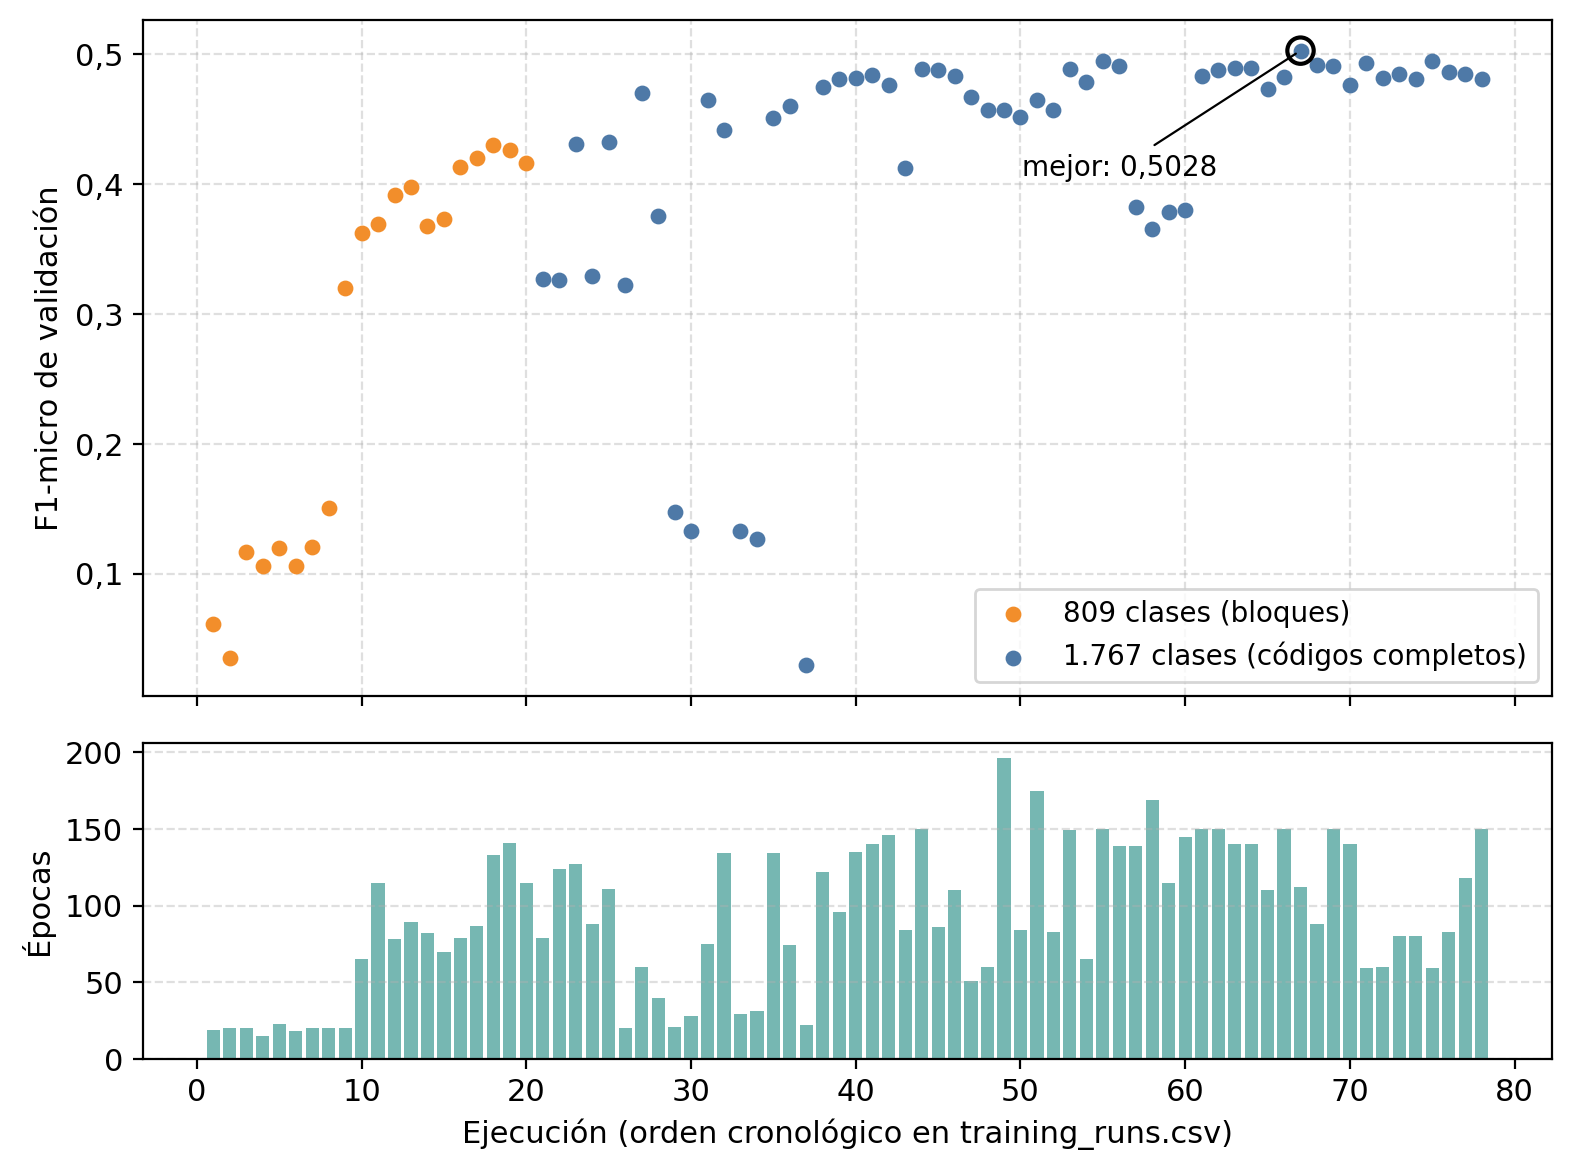
\includegraphics[width=\textwidth]{figs/all_trainings_graph}
\caption{F1-micro de validación (arriba) y épocas ejecutadas (abajo) de cada ejecución, en orden cronológico. Azul: 1.767 clases; naranja: 809 clases. El círculo marca la mejor ejecución con 1.767 clases. Generada con \texttt{make ai-tfg-figures} (\texttt{ai\_engine/plot\_runs.py}) a partir de \texttt{model/training\_runs.csv}.}
\label{fig:all-trainings}
\end{figure}

\section{Optimización específica del MAP}
\label{sec:anexoF-map}

Las 62~ejecuciones anteriores optimizaron el F1-micro, por las razones expuestas en el capítulo de desarrollo. El MAP por documento, sin embargo, es la métrica oficial del \emph{benchmark} CodiEsp y la única homogénea con los sistemas participantes, por lo que se realizó una serie de experimentos dirigidos específicamente a mejorarla.

\paragraph{Procedencia de las cifras de esta sección.}
El mismo modelo aparece con dos valores según la pasada de evaluación. Las cifras del modelo del paso~36 (MAP de prueba 0,4373; F1-micro 0,4887) proceden de \texttt{eval\_test.py} en precisión completa y fueron las cifras titulares hasta que la comparación de candidatos en prueba (Anexo~\ref{cap:AnexoH}, sección~\ref{sec:anexoH-candidatos}) promocionó \texttt{zlpr-map}; el cuerpo de la memoria cita ahora 0,454 y 0,495 para ese modelo. Las tablas de esta sección son anteriores a esa promoción y \textbf{comparan varias ejecuciones entre sí} con \texttt{ensemble\_eval.py}, en precisión reducida, donde el modelo del paso~36 da 0,4342 en prueba y 0,4343 en validación (\texttt{eval\_paso40.json}). Cada tabla indica sus ficheros de origen, todos ellos salidas de ese guion, y usa esa fila para el paso~36. Las pasadas difieren entre sí en la tercera o cuarta cifra decimal (por ejemplo, 37a da 0,4389 en \texttt{ensemble\_eval.json} y 0,4390 en \texttt{ensemble\_eval5.json}; la ejecución 41b da 0,4533 y 0,4535 en dos pasadas). Esas diferencias no alteran ninguna conclusión, pero mezclar ambas procedencias al citar produciría una contradicción aparente. Salvo indicación expresa, el MAP de las tablas es el de prueba sobre el \emph{gold} completo; los diferenciales derivados se calculan dentro de una misma procedencia.

\subsection{Variabilidad estocástica como referencia}

Antes de atribuir una mejora a cualquier cambio es necesario conocer el ruido del proceso. Dos ejecuciones con configuración \textbf{idéntica} (\texttt{20260530T030233Z} y \texttt{20260530T134649Z}) obtuvieron MAP de 0{,}5442 y 0{,}5317 en validación: una dispersión de \textbf{1{,}25~puntos porcentuales} atribuible únicamente a la inicialización aleatoria y al no determinismo del entrenamiento en GPU. Esa cifra está medida sobre el MAP de validación restringido al vocabulario del modelo, que es la métrica que registraba el entrenamiento en ese momento, y sobre dos ejecuciones. La subsección~\ref{sec:anexoF-distribuciones} la sustituye por una estimación con cinco réplicas sobre la métrica que de verdad decide, el MAP del \emph{gold} completo en prueba: desviación típica de 0{,}0051 y rango de 1{,}06~pp. Con cualquiera de las dos lecturas la conclusión operativa es la misma: una diferencia inferior al punto porcentual no puede atribuirse con seguridad a un cambio a partir de una sola ejecución.

\subsection{Selección de checkpoint por MAP}

Hasta este punto, el mejor \emph{checkpoint} y el planificador de la tasa de aprendizaje (\emph{scheduler}) \texttt{ReduceLROnPlateau} se gobernaban por el F1-micro de validación. Se incorporó el parámetro \texttt{--select\_metric} para poder guiarlos por el MAP, y se registró además el MAP de cada época en el historial de entrenamiento, que hasta entonces no se almacenaba.

El análisis del historial de la ejecución de control mostró que el margen disponible era pequeño: el MAP máximo (0{,}5501, época~88) apenas superaba en 0{,}24~pp al MAP de la época elegida por F1 (0{,}5477, época~103), y permanecía prácticamente plano entre las épocas~70 y~124. La ejecución completa (Tabla~\ref{tab:map-experiments}) apunta a que el cambio es contraproducente: guiar el planificador por una métrica plana parece degradar la trayectoria de aprendizaje completa.

\subsection{Calibración entre clases}

El MAP evalúa el \emph{ranking} de códigos dentro de cada documento, de modo que el \texttt{pos\_weight} por clase (que desplaza los \emph{logits} de cada código en distinta magnitud) podría estar distorsionando esa comparación. Se redujo \texttt{pos\_weight\_cap} de 10 a 3, con resultado también negativo tanto en MAP como en F1. La Tabla~\ref{tab:map-experiments} recoge ambos experimentos junto con la ejecución de control.

\begin{table}[h]
\centering
\caption{Experimentos dirigidos a mejorar el MAP. Todos parten de la configuración de producción (paso~36). MAP de validación restringido al vocabulario del modelo y F1-micro de validación, de \texttt{model/\allowbreak ensemble\_eval.json}. Generada con \texttt{python3 ensemble\_eval.py --ckpts} \emph{checkpoints} \texttt{--labels} etiquetas (sin objetivo de \texttt{make}); la salida es ese JSON.}
\label{tab:map-experiments}
\begin{tabular}{lP{6.0cm}cc}
\hline
\textbf{Ejec.} & \textbf{Cambio respecto a producción} & \textbf{MAP val} & \textbf{F1-micro val} \\
\hline
37ctrl & Ninguno (control, otra semilla) & 0{,}5477 & 0{,}4884 \\
37a & \texttt{select\_metric=map\_macro} & 0{,}5365 & 0{,}4902 \\
37b & \texttt{select\_metric=map\_macro} + \texttt{pos\_weight\_cap=3} & 0{,}5202 & 0{,}4743 \\
\hline
\end{tabular}
\end{table}

\subsection{Observación incidental: promediado de las ejecuciones}

Una variabilidad de 1{,}25~pp sugiere que reducir la varianza puede ser más rentable que perseguir configuraciones marginalmente mejores. Para comprobarlo se promediaron las probabilidades de salida de los tres \emph{checkpoints} anteriores, con los resultados de la Tabla~\ref{tab:map-ensemble}. Esta prueba tiene un alcance limitado: los tres \emph{checkpoints} no se entrenaron para combinarse, sino que persiguen objetivos distintos (un control y dos variantes que, individualmente, resultaron peores). No se trata, por tanto, de un sistema de combinación diseñado ni evaluado como tal, sino de una comprobación posterior sobre los modelos disponibles. Por ese motivo el resultado no se reporta como resultado de este trabajo ni se emplea en la comparación con el \emph{benchmark}, que utiliza el modelo de producción.

\begin{table}[h]
\centering
\caption{MAP por documento sobre el conjunto de prueba: modelos individuales frente a su promedio. El promedio no constituye un sistema propuesto (véase el texto). Las filas 37a y promedio proceden de \texttt{model/\allowbreak ensemble\_eval.json}; la fila del paso~36, de \texttt{model/\allowbreak eval\_paso40.json} (mismo guion, otra pasada). Generada con \texttt{python3 ensemble\_eval.py} (sin objetivo de \texttt{make}).}
\label{tab:map-ensemble}
\begin{tabular}{lcc}
\hline
\textbf{Modelo} & \textbf{MAP (gold completo)} & \textbf{MAP (vocabulario)} \\
\hline
Producción (paso~36) & 0{,}4342 & 0{,}5326 \\
Mejor individual (37a) & 0{,}4389 & 0{,}5393 \\
Promedio de los 3 & 0{,}4683 & 0{,}5728 \\
\hline
\end{tabular}
\end{table}

El promedio supera al modelo de producción en 3{,}41~pp de MAP sobre el gold completo y al mejor modelo individual en 2{,}9~pp, más de dos veces la dispersión entre semillas (1,06~pp de rango, Tabla~\ref{tab:map-distribuciones}), y el efecto se reproduce en validación. El coste sería triplicar el tiempo de inferencia y el espacio de almacenamiento, incompatible con el requisito de latencia del sistema. La conclusión que cabe extraer es metodológica: existe margen de mejora por esta vía, y diseñar y evaluar una combinación de modelos de forma rigurosa queda planteado como trabajo futuro.

\subsection{Destilación del promedio}

El promediado deja una pregunta abierta: si la ganancia existe pero no cabe en el presupuesto de inferencia, ¿puede transferirse a un único modelo? La vía estándar es la destilación de conocimiento~\cite{hinton2015distilling}: entrenar un clasificador nuevo (alumno) contra las probabilidades que produce el promedio (profesor), en lugar de contra las etiquetas binarias del corpus. La hipótesis es que las probabilidades del profesor contienen información que las etiquetas no tienen (sobre todo en los negativos, donde el orden relativo entre códigos plausibles y códigos absurdos es precisamente lo que mide el MAP) y que el alumno puede aprenderla conservando el coste de inferencia de un solo modelo.

Se amplió primero el promedio de tres a cinco ejecuciones (Tabla~\ref{tab:map-distill}) y se entrenó el alumno con una pérdida mixta $\alpha \cdot \mathcal{L}_{\text{blanda}} + (1-\alpha) \cdot \mathcal{L}_{\text{dura}}$ con $\alpha = 0{,}5$, siendo $\mathcal{L}_{\text{blanda}}$ la entropía cruzada binaria contra las probabilidades del profesor.

\begin{table}[h]
\centering
\caption{Destilación del promedio de cinco ejecuciones. MAP por documento sobre el gold completo. Rango y promedio de \texttt{model/\allowbreak ensemble\_eval5.json}, alumno de \texttt{model/\allowbreak eval\_distill.json} y paso~36 de \texttt{model/\allowbreak eval\_paso40.json}. Generada con \texttt{python3 ensemble\_eval.py} (sin objetivo de \texttt{make}).}
\label{tab:map-distill}
\begin{tabular}{P{6.0cm}cc}
\hline
\textbf{Modelo} & \textbf{MAP validación} & \textbf{MAP prueba} \\
\hline
Producción (paso~36) & 0{,}4343 & 0{,}4342 \\
Cinco ejecuciones previas disponibles (rango)$^{*}$ & 0{,}4166--0{,}4442 & 0{,}4192--0{,}4421 \\
Promedio de las cinco & 0{,}4715 & 0{,}4778 \\
Alumno destilado & 0{,}4299 & 0{,}4354 \\
\hline
\end{tabular}

\vspace{2mm}
{\footnotesize $^{*}$ Dos de esas cinco ejecuciones no eran réplicas de la configuración de producción sino variantes descartadas, lo que rebajaba la media del grupo. La subsección~\ref{sec:anexoF-distribuciones} documenta el error y rehace la comparación con el grupo corregido.}
\end{table}

El alumno no recupera ganancia apreciable: su MAP de prueba queda dentro del rango de las ejecuciones individuales y 4{,}2~pp por debajo del profesor. El diagnóstico está en las probabilidades del profesor sobre el conjunto de entrenamiento, que es donde el alumno aprende: la probabilidad media asignada a los códigos positivos es del 97~\% y el 99{,}5~\% de ellos supera el 0{,}9. Con 500 documentos y 150~épocas, los profesores prácticamente memorizan el corpus de entrenamiento, de modo que sus probabilidades se reducen a las etiquetas binarias y la pérdida blanda no aporta señal adicional. La estructura fina de los negativos, que era la apuesta del experimento, tampoco basta: con $\alpha=0{,}5$ y probabilidades negativas del orden de $10^{-3}$, ese término queda aplastado por la contribución de los positivos.

La lección no es que la destilación no funcione, sino que no funciona \emph{en este régimen}: exige un profesor que generalice sobre los datos que ve el alumno, y con 500 documentos el profesor no generaliza sobre ellos, los memoriza. Destilar sobre un corpus no etiquetado y disjunto del de entrenamiento (donde el profesor sí produciría probabilidades informativas) es la variante que quedaría por probar, y requiere textos clínicos adicionales de los que este trabajo no dispone.

\subsection{Alinear la pérdida con la métrica}
\label{sec:anexoF-alineacion}

Los experimentos anteriores comparten un supuesto que conviene revisar: todos ajustan el proceso de entrenamiento (qué \emph{checkpoint} se elige, cómo se pondera cada clase, con qué semilla se arranca) manteniendo intacta la función de pérdida. Y esa función es una entropía cruzada binaria que trata cada uno de los 1.767 códigos como un problema independiente: optimiza que la probabilidad de cada código esté bien calibrada por separado. El MAP mide algo distinto, que los códigos correctos de un informe queden por encima de los incorrectos \emph{de ese mismo informe}. Un ajuste de hiperparámetros difícilmente puede corregir esa desalineación, porque el objetivo que se minimiza sigue siendo otro. A esto se suma el diagnóstico acumulado en las secciones anteriores: el ruido entre semillas idénticas (en torno a 1~pp sobre el conjunto de prueba, según la estimación con réplicas de la subsección~\ref{sec:anexoF-distribuciones}) es del orden del efecto de cualquier cambio de hiperparámetro ensayado, y lo que más ha movido el MAP hasta ahora (promediar varias ejecuciones, $+4{,}36$~pp sobre el paso~36 con cinco ejecuciones) es inviable en producción por coste de inferencia.

De ahí salen tres ejecuciones, cada una atacando uno de esos tres diagnósticos. Todas parten de la configuración de producción y modifican un solo elemento, de forma que sus efectos sean atribuibles por separado, y ninguna altera el coste de inferencia: los tres cambios viven exclusivamente en el entrenamiento.

\subsubsection*{Ejecución 40a: pérdida listwise por documento (ZLPR)}

\textbf{Diagnóstico que ataca.} La desalineación entre pérdida y métrica.

\textbf{Mecanismo.} Se añade a la entropía cruzada el término~\cite{su2022zlpr}
\[
\mathcal{L}_{\text{ZLPR}} = \log\Big(1 + \sum_{j \in \text{neg}} e^{z_j}\Big) + \log\Big(1 + \sum_{i \in \text{pos}} e^{-z_i}\Big),
\]
mínimo cuando todos los códigos correctos de un documento superan a todos los incorrectos del mismo documento, sin exigir ningún valor absoluto concreto a ninguno. Es la traducción directa del MAP a una función derivable. El peso, 0{,}1, se fijó midiendo ambos términos en una ejecución de prueba de una época: con ese factor la entropía cruzada aporta 0{,}74 y el término de ordenación 1{,}02, escalas comparables.

\textbf{Qué se espera.} Es la que actúa sobre la causa y no sobre un síntoma, así que es la candidata con mayor recorrido: una mejora de 2~a~4~pp de MAP la situaría por encima del ruido. El riesgo simétrico es que empeore el F1-micro, porque una pérdida que solo exige orden relativo no obliga a calibrar las probabilidades, y el F1 depende de un umbral absoluto. Un resultado con MAP claramente mejor y F1 algo peor sería informativo, no un fracaso: el umbral se reajusta después con el barrido de validación.

\textbf{Qué la refutaría.} Un MAP dentro del rango del grupo de referencia indicaría que con 500 documentos el modelo no tiene capacidad de aprender orden fino aunque se le pida explícitamente, y que el cuello de botella es la cantidad de datos, no el objetivo.

\subsubsection*{Ejecución 40b: media móvil exponencial de los pesos}

\textbf{Diagnóstico que ataca.} Que la ganancia más clara medida hasta ahora venga de reducir varianza, y que la forma conocida de hacerlo (promediar ejecuciones) multiplique el coste de inferencia.

\textbf{Mecanismo.} Se mantiene una media móvil de los pesos entrenables a lo largo del entrenamiento y se evalúa y guarda esa media, no los pesos del último paso. Persigue el mismo efecto que el promediado de modelos, pero dentro de una sola trayectoria: los puntos que promedia están en la misma cuenca de la función de pérdida por construcción, y el resultado sigue siendo un único modelo con el coste de inferencia de siempre. El decaimiento, $0{,}99$, se fija a partir de los pasos reales del optimizador: 500 documentos con \emph{batch} efectivo de 32 dan unos 15 pasos por época, de modo que $0{,}99$ promedia una ventana de unos 100 pasos (siete épocas), mientras que el $0{,}999$ habitual en corpus grandes abarcaría media ejecución y quedaría permanentemente rezagado.

\textbf{Qué se espera.} Es la apuesta más conservadora y la de mayor valor práctico si sale: recupera parte de los $+4{,}36$~pp del promediado sin ninguno de sus costes. La expectativa razonable es una fracción de esa ganancia, del orden de 1~a~2~pp, porque promedia puntos correlacionados de una misma trayectoria en lugar de modelos independientes. Debería además reducir la dispersión entre ejecuciones, que es en sí mismo un resultado útil: gran parte de la dificultad de esta serie de experimentos viene de que el ruido tapa los efectos.

\textbf{Qué la refutaría.} Una media que iguale o empeore al último \emph{checkpoint} indicaría que la trayectoria no oscila alrededor de un óptimo sino que sigue avanzando hasta el final, en cuyo caso promediar solo introduce retraso.

\subsubsection*{Ejecución 40c: R-Drop}

\textbf{Diagnóstico que ataca.} La escasez de datos: 500 documentos para 1.767 códigos, la mayoría de ellos con menos de tres ejemplos positivos.

\textbf{Mecanismo.} Cada informe se procesa dos veces con máscaras de \emph{dropout} distintas y se penaliza la divergencia entre ambas salidas~\cite{wu2021rdrop}. Es regularización que no consume etiquetas: aprovecha los documentos disponibles sin depender de cuántos positivos tenga cada código. La divergencia se promedia sobre las clases en lugar de sumarse, lo que la deja tres órdenes de magnitud por debajo de la convención habitual; $\alpha=5$ se fijó con la misma ejecución de prueba, para que la regularización pese en torno a una cuarta parte de la entropía cruzada.

\textbf{Qué se espera.} Es la más indirecta de las tres (mejora la generalización en general, no el orden dentro del documento en particular), así que se espera un efecto menor, de 0~a~2~pp, y con más probabilidad de quedar dentro del ruido. Se incluye porque es el mecanismo que ataca más directamente la limitación de fondo del problema, y porque su coste es únicamente de entrenamiento: duplica el tiempo por lote, pero no cambia nada en inferencia.

\textbf{Qué la refutaría.} Cualquier resultado dentro del rango de control, que es el desenlace más probable de los tres.

\subsubsection*{Condiciones de ejecución y criterio de decisión}

Las tres se lanzan en paralelo sobre la misma GPU (RTX 4080, 16~GB), cada una con su propio directorio de salida para que no compitan por los mismos artefactos ni sobrescriban la configuración de producción. Con las tres simultáneas la ocupación de memoria es de 12{,}3~GB y el tiempo por paso pasa de unos 0{,}25~s a 0{,}6 a 0{,}9~s, de modo que la concurrencia no reduce el tiempo total de cómputo: reparte el mismo trabajo, con la ventaja de que los tres resultados llegan a la vez y son comparables entre sí.

El criterio de decisión se fija \emph{antes} de ver los resultados, para que la comparación no se acomode a ellos: una ejecución solo cuenta como mejora si su MAP supera el \textbf{máximo} del grupo de referencia (0{,}4442 en validación y 0{,}4421 en prueba), no su media. Con una dispersión entre semillas idénticas de 1,06~pp de rango sobre las cinco réplicas de control en prueba (Tabla~\ref{tab:map-distribuciones}; en el momento de fijar el criterio solo se disponía de la estimación de 1,25~pp con dos ejecuciones, subsección~\ref{sec:anexoF-map}), superar la media es difícil de distinguir de haber tenido suerte con el sorteo. Una ejecución que supere ese listón tampoco se dará por buena hasta repetirse con otra semilla.

\subsubsection*{Resultados}

La Tabla~\ref{tab:map-paso40} recoge el MAP por documento de las tres ejecuciones sobre validación y prueba, junto con la ejecución de producción medida en la misma pasada y el rango del grupo de referencia. Todas las cifras proceden de la misma pasada (\texttt{model/\allowbreak eval\_paso40.json}, generada con \texttt{python3 ensemble\_eval.py}, sin objetivo de \texttt{make}) y son por tanto comparables entre sí; difieren en la tercera cifra decimal de las reportadas en otras secciones porque la inferencia se realiza con precisión reducida.

\begin{table}[h]
\centering
\caption[Paso 40: MAP por documento sobre el gold completo]{Paso 40: MAP por documento sobre el gold completo. El grupo de referencia es el que se empleó en el momento de estos experimentos; la subsección~\ref{sec:anexoF-distribuciones} lo corrige. Datos de \texttt{model/\allowbreak eval\_paso40.json}, generada con \texttt{python3 ensemble\_eval.py} (sin objetivo de \texttt{make}).}
\label{tab:map-paso40}
\begin{tabular}{P{5.2cm}ccc}
\hline
\textbf{Ejecución} & \textbf{MAP validación} & \textbf{MAP prueba} & \textbf{F1-micro prueba} \\
\hline
Producción & 0{,}4343 & 0{,}4342 & 0{,}4872 \\
Ejecuciones previas disponibles (rango)$^{*}$ & 0{,}4166--0{,}4442 & 0{,}4192--0{,}4421 & no calculado \\
\hline
40a (ZLPR) & 0{,}4369 & \textbf{0{,}4440} & \textbf{0{,}4917} \\
40b (media móvil) & 0{,}4342 & 0{,}4313 & 0{,}4747 \\
40c (R-Drop) & 0{,}4237 & 0{,}4294 & 0{,}4813 \\
\hline
\end{tabular}

\vspace{2mm}
{\footnotesize $^{*}$ Grupo de referencia con el defecto descrito en la nota de la Tabla~\ref{tab:map-distill}; la subsección~\ref{sec:anexoF-distribuciones} lo corrige.}
\end{table}

\textbf{40c (R-Drop) queda refutada} en los términos previstos: su MAP cae dentro del rango de control en ambos conjuntos. La regularización adicional no compensa en un régimen donde el modelo ya está fuertemente restringido (solo cuatro capas entrenables de veinticuatro al comenzar) y el \emph{dropout} de 0{,}3 ya cumple ese papel.

\textbf{40b (media móvil) queda refutada por la razón concreta que se había anticipado}: se estableció de antemano que la media fallaría si la trayectoria, en lugar de oscilar alrededor de un óptimo, seguía avanzando hasta el final. Es lo que ocurrió: la ejecución agotó las 150~épocas sin activar nunca la parada temprana, con su mejor F1 en la época~144, de modo que la trayectoria nunca llegó a estabilizarse en torno a un óptimo y promediar los pesos de las siete épocas anteriores solo introduce retraso respecto al punto más avanzado. La media móvil es una herramienta para trayectorias que han convergido, y esta no lo había hecho.

\textbf{40a (ZLPR) supera el criterio sobre el conjunto de prueba} (0{,}4440 frente al máximo de control de 0{,}4421) y lo hace sin el efecto adverso que se temía: el F1-micro no se degrada y es el mejor de las cuatro ejecuciones. Que la pérdida de ordenación mejore simultáneamente el orden y la clasificación por umbral sugiere que ambos objetivos no competían tanto como se suponía. Sobre validación, en cambio, el resultado se queda en 0{,}4369, por debajo del máximo de control. Con una dispersión entre semillas de 1,06~pp de rango (Tabla~\ref{tab:map-distribuciones}), una ventaja de 0{,}19~pp en un solo conjunto y de una sola ejecución no basta para declarar una mejora, y así se hace constar.

Hay además una razón para pensar que la ejecución no llegó a su techo. La parada temprana y el planificador se gobiernan por el F1-micro, y bajo esta pérdida ambas métricas dejan de moverse a la vez: el entrenamiento se detuvo en la época~59 de~150 con el F1 estancado desde la~39, pero con el MAP de validación en 0{,}554 y todavía en ascenso. El \emph{checkpoint} guardado es el del mejor F1, no el del mejor MAP. La sección~\ref{sec:anexoF-map} había descartado gobernar la selección por el MAP porque, bajo entropía cruzada, esa métrica era plana entre las épocas~70 y~124 y guiaba mal al planificador; bajo una pérdida que empuja el MAP explícitamente, esa objeción deja de aplicarse. De ahí las dos primeras ejecuciones de continuación (41a y 41b): una que repite 40a con semilla distinta y sin otro cambio, y otra que la repite con selección por MAP, para separar el efecto del sorteo del de la selección.

\subsubsection*{Ejecuciones de continuación}

Las dos primeras ejecuciones de continuación (41a y 41b) separan la variabilidad aleatoria del efecto de la selección, y cada una cae del lado que el criterio previo había fijado; una tercera (41c, otra semilla) replica 41b y se comenta más abajo. La Tabla~\ref{tab:map-paso41} recoge los resultados de las dos primeras junto a la referencia.

\begin{table}[h]
\centering
\caption{Ejecuciones de continuación de 40a: MAP por documento sobre el gold completo. El rango de control es el mismo de la Tabla~\ref{tab:map-paso40}. Todas las cifras de 41a y 41b proceden de \texttt{model/\allowbreak eval\_paso41.json}; la misma ejecución 41b da 0,4535 en \texttt{model/\allowbreak eval\_paso41b.json}, la pasada que usan las Tablas~\ref{tab:map-distribuciones} y~\ref{tab:map-fusion}. Generada con \texttt{python3 ensemble\_eval.py} (sin objetivo de \texttt{make}).}
\label{tab:map-paso41}
\begin{tabular}{P{5.2cm}ccc}
\hline
\textbf{Ejecución} & \textbf{MAP validación} & \textbf{MAP prueba} & \textbf{F1-micro prueba} \\
\hline
Ejecuciones previas disponibles (rango)$^{*}$ & 0{,}4166--0{,}4442 & 0{,}4192--0{,}4421 & no calculado \\
40a original & 0{,}4369 & 0{,}4440 & 0{,}4917 \\
\hline
41a: 40a con semilla fija & 0{,}4257 & 0{,}4326 & 0{,}4801 \\
41b: 40a con \texttt{select\_metric=map\_macro} & \textbf{0{,}4451} & \textbf{0{,}4533} & \textbf{0{,}4931} \\
\hline
\end{tabular}

\vspace{2mm}
{\footnotesize $^{*}$ Grupo de referencia con el defecto descrito en la nota de la Tabla~\ref{tab:map-distill}; la subsección~\ref{sec:anexoF-distribuciones} lo corrige.}
\end{table}

\textbf{41a refuta a 40a.} Repetida con otra semilla y sin ningún otro cambio, la ejecución cae dentro del rango de control en los dos conjuntos (0,4257 en validación y 0,4326 en prueba). La ventaja de 0,19~pp que 40a mostraba sobre el máximo de control es, por tanto, compatible con el azar. Es el desenlace que la sección anterior se había comprometido a aceptar, y la razón por la que se exigía la replicación antes de dar nada por bueno: sin ella, 40a habría entrado en la memoria como una mejora no replicada.

\textbf{41b supera el criterio en los dos conjuntos.} Gobernar la selección del \emph{checkpoint} y el planificador por el MAP, en lugar de por el F1-micro, da 0,4451 en validación (máximo de control 0,4442) y 0,4533 en prueba (0,4535 en la otra pasada; máximo de control 0,4421), esto es 1,12~pp por encima del control y 0,93~pp por encima de la propia 40a. Mejora además el F1-micro de prueba respecto al modelo de producción (0,4931 frente a 0,4872), de modo que la mejora de ordenación no se paga con la clasificación por umbral. Es el único cambio de la serie que supera el criterio fijado de antemano en los dos conjuntos, y es coherente con la hipótesis con la que se diseñó: la objeción de la sección~\ref{sec:anexoF-map} contra seleccionar por MAP (que bajo entropía cruzada esa métrica es plana y guía mal al planificador) deja de aplicarse cuando la pérdida empuja el MAP de forma explícita.

\textbf{No se da por consolidado con una sola ejecución.} El mismo criterio que permite descartar 40a obliga a no aceptar 41b hasta replicarla, y la replicación no la sostuvo: repetida con otra semilla, la misma configuración (41c, \texttt{model/\allowbreak eval\_paso41c.json}) obtuvo 0{,}4383 sobre prueba frente a los 0{,}4533 de la original. Es un segundo caso con la misma forma que el primero, aunque la subsección siguiente lo matiza con más réplicas. La conclusión metodológica es que en este régimen una ejecución individual aporta poca evidencia, y que la comparación tiene que hacerse entre distribuciones.

\subsection{Comparación entre distribuciones}
\label{sec:anexoF-distribuciones}

Al construir el grupo de control apareció un error que arrastraban las secciones anteriores. Las cinco ejecuciones que se venían usando como control no eran réplicas de la configuración de producción: dos de ellas eran las variantes fallidas 37a y 37b, que cambiaban la métrica de selección y el \texttt{pos\_weight}. La peor de todas, 37b con 0{,}4192, rebajaba la media del grupo e inflaba artificialmente cualquier efecto medido contra ella. El control legítimo eran tres réplicas, que se ampliaron a cinco con dos ejecuciones adicionales, y el grupo experimental se amplió a cuatro semillas. La Tabla~\ref{tab:map-distribuciones} recoge ambas distribuciones. El propio modelo de producción queda \emph{fuera} del grupo de control: se eligió en su día por ser el mejor de muchas ejecuciones, de modo que incluirlo sesgaría la comparación.

\begin{table}[h]
\centering
\caption{MAP por documento sobre el conjunto de prueba (gold completo): réplicas de la configuración de producción frente a ZLPR con selección por MAP. Control: 37ctrl, 38b y 38c de \texttt{model/\allowbreak ensemble\_eval5.json} y las réplicas 303 y 404 de \texttt{model/\allowbreak eval\_ctrl.json}. ZLPR con selección por MAP: 41b de \texttt{model/\allowbreak eval\_paso41b.json}, 41c de \texttt{model/\allowbreak eval\_paso41c.json} y las semillas 101 y 202 de \texttt{model/\allowbreak eval\_paso42.json}. Estadísticos calculados con \texttt{python3 compare\_runs.py} (sin objetivo de \texttt{make}).}
\label{tab:map-distribuciones}
\begin{tabular}{lcccc}
\hline
\textbf{Grupo} & \textbf{n} & \textbf{Media} & \textbf{Desv. típica} & \textbf{Rango} \\
\hline
Control (réplicas de producción) & 5 & 0{,}4359 & 0{,}0051 & 0{,}4315--0{,}4421 \\
ZLPR + selección por MAP & 4 & \textbf{0{,}4466} & 0{,}0070 & 0{,}4383--0{,}4535 \\
\hline
\end{tabular}
\end{table}

La diferencia de medias es de $+1{,}08$~pp. La prueba $t$ de Welch, que no presupone varianzas iguales, da $t = 2{,}59$ con 5{,}4~grados de libertad y $p = 0{,}045$, con un tamaño del efecto de $d = 1{,}81$ y un intervalo de confianza al 95~\% de $[+0{,}03, +2{,}12]$~pp. Las cuatro ejecuciones con la pérdida de ordenación superan la media del control y tres superan también su máximo. Es la primera diferencia de la serie que alcanza significación nominal (\(p<0{,}05\)), con la salvedad que sigue.

Esa afirmación debe leerse con cautela. Con cuatro y cinco ejecuciones por grupo, un $p$ de 0{,}045 es evidencia moderada y no concluyente, y el extremo inferior del intervalo roza el cero, como corresponde a un $p$ tan próximo al umbral. La ganancia queda además muy por debajo de los $+4{,}36$~pp del promediado de modelos. Su interés es que, a diferencia del promediado, no cuesta nada en inferencia.

Una explicación plausible de por qué ninguna de las dos piezas funcionaba por separado es la siguiente. La pérdida de ordenación desacopla las dos métricas: bajo entropía cruzada, F1-micro y MAP se estancan a la vez, mientras que con el término listwise el modelo sigue reordenando códigos dentro de cada documento mucho después de que las probabilidades absolutas hayan dejado de moverse. La ejecución 40a lo dejó a la vista, como se ha descrito: se detuvo con el MAP aún en ascenso y guardó el \emph{checkpoint} de veinte épocas antes del mejor. Y por eso la selección por MAP, descartada en la sección~\ref{sec:anexoF-map} porque bajo entropía cruzada esa métrica era plana y guiaba mal al planificador, vuelve a tener sentido: deja de ser plana precisamente porque es la que se está optimizando. Una genera el progreso y la otra lo conserva.

\subsection{Fusión con el baseline de diccionario}
\label{sec:anexoF-fusion}

Toda la serie anterior comparte una limitación de partida: busca la mejora dentro del modelo neuronal, ajustando su pérdida, su selección de \emph{checkpoint} o su regularización. El techo de esa vía quedó medido en algo más de un punto porcentual. La alternativa es añadir una fuente de evidencia que el modelo no tiene, y el sistema ya dispone de una: el clasificador de diccionario descrito en el capítulo de desarrollo (sección~\ref{sec:diccionario}), que detecta bloques CIE-10 por coincidencia léxica sobre el informe.

La combinación se plantea sobre las puntuaciones y no sobre las listas de salida. A cada código se le suma una bonificación proporcional a la confianza con que el diccionario ha detectado su bloque:
\[
s_c = z_c + \beta \cdot \text{conf}(\text{bloque}(c)),
\]
con $\beta$ ajustado exclusivamente sobre validación. El barrido se extendió hasta $\beta = 64$, para comprobar que el óptimo ($\beta = 6$) es interior y no un artefacto del borde de la rejilla explorada: por encima de ese valor el MAP de validación decae, de 0{,}5507 con $\beta = 6$ a 0{,}5370 con $\beta = 64$ (\texttt{model/\allowbreak fusion\_sweep.json}). La Tabla~\ref{tab:map-fusion} recoge el resultado de la combinación frente a cada sistema por separado.

\begin{table}[h]
\centering
\small
\caption[Todas las configuraciones de los dos motores, medidas sobre el conjunto de prueba y en el mismo espacio de 1.767 códigos completos]{Todas las configuraciones de los dos motores, medidas sobre el conjunto de prueba y en el mismo espacio de 1.767 códigos completos. El umbral de decisión de cada configuración de diccionario/fusión se ajusta sobre validación y se aplica sin retocar a prueba; las filas \texttt{both} no lo optimizan, porque concatenan lo que cada motor ya decide con su propio umbral de producción (nota al pie). Las filas del modelo desplegado y del diccionario proceden de \texttt{model/\allowbreak comparativa\_motores.json}, generado con \texttt{make ai-comparativa-motores} (\texttt{ai\_engine/\allowbreak motores\_eval.py}, precisión completa); el barrido de $\beta$, de \texttt{model/\allowbreak fusion\_sweep.json} (misma orden). Las filas del modelo del paso~36 proceden de \texttt{model/\allowbreak comparativa\_motores\_paso36.json}, generado con el mismo guion y el mismo \emph{checkpoint} (nota al pie).}
\label{tab:map-fusion}
\begin{tabular}{P{6.4cm}rrrr}
\hline
\textbf{Configuración} & \textbf{MAP} & \textbf{P} & \textbf{R} & \textbf{F1-micro} \\
\hline
Diccionario solo & 0{,}1452 & 0{,}188 & 0{,}791 & 0{,}304 \\
\hline
Modelo del paso~36 solo & 0{,}4372 & 0{,}517 & 0{,}461 & 0{,}487 \\
\quad + diccionario concatenado (\texttt{both}) & no aplica & 0{,}167 & 0{,}859 & 0{,}280 \\
\quad + diccionario fusionado & \textbf{0{,}5468} & 0{,}633 & 0{,}571 & \textbf{0{,}600} \\
\hline
Modelo desplegado (\texttt{zlpr-map}) solo & 0{,}4539 & 0{,}552 & 0{,}452 & 0{,}497 \\
\quad + diccionario concatenado (\texttt{both})$^{\dagger}$ & no aplica & 0{,}171 & 0{,}851 & 0{,}285 \\
\quad + diccionario fusionado & \textbf{0{,}5536} & 0{,}642 & 0{,}582 & \textbf{0{,}610} \\
\hline
\end{tabular}

\vspace{2mm}
{\footnotesize $^{\dagger}$ Fila del modelo desplegado, generada con \texttt{make ai-comparativa-motores} (\texttt{ai\_engine/motores\_eval.py}), que concatena las predicciones de cada motor con su propio umbral de producción (clasificador: 0,2; diccionario: cualquier bloque con un patrón que haga match) y queda en \texttt{model/comparativa\_motores.json} (\texttt{ambos\_concatenado}). Las filas del modelo del paso~36 salen de la misma herramienta con ese \emph{checkpoint}, con \texttt{make ai-comparativa-motores MODEL\_FILE=classifier.pt THRESHOLDS\_FILE=thresholds.json SUFIJO=\_paso36}, y quedan en \texttt{model/\allowbreak comparativa\_motores\_paso36.json}; la fusión usa el umbral elegido en validación (2,753), por lo que su MAP (0,5468) difiere ligeramente del 0,5449 de \texttt{models.json}, que emplea el umbral de configuración (2,9).}
\end{table}

La tabla contiene tres lecturas que conviene separar.

\textbf{El diccionario por sí solo es un mal sistema en este espacio de etiquetas} (MAP 0{,}1452), porque predice bloques y asigna la misma puntuación a todos los códigos que cuelgan de un mismo bloque, de modo que no establece ningún orden dentro de él. Su \emph{recall} de 0{,}791 revela sin embargo dónde está su valor: reconoce casi todo lo que hay que reconocer, pero no sabe discriminar. Conviene precisar que esa cifra está medida sobre el espacio de 1.767 códigos completos, que es el de esta tabla; evaluado en su propio espacio de bloques, como se hace en el capítulo de desarrollo, el mismo clasificador obtiene 0{,}461 de MAP y 0{,}672 de F1. No son resultados contradictorios sino dos tareas distintas.

\textbf{La concatenación de ambos motores, que es lo que el sistema ofrecía como modo \texttt{both}, empeora a los dos.} Con el modelo desplegado su F1 de 0{,}285 queda por debajo del modelo solo (0{,}497) y del diccionario solo en el espacio de esta tabla (0{,}304), y con el del paso~36 es de 0{,}302 frente a 0{,}487. Unir los conjuntos predichos hereda los falsos positivos de ambos sin ningún criterio para arbitrar entre ellos: con el modelo desplegado el \emph{recall} sube a 0{,}851 y la precisión se desploma a 0{,}171. Tampoco admite MAP, porque dos listas concatenadas no definen una ordenación única. El modo existía para que el cliente viera el origen de cada predicción, no como sistema de combinación, y esta medición desaconseja usarlo como tal.

\textbf{La fusión de puntuaciones sí combina.} Con el modelo del paso~36 sube el MAP en 11{,}0~pp (de 0{,}4372 a 0{,}5468) y el F1 en 11{,}3~pp (de 0{,}487 a 0{,}600); con el modelo desplegado, en 9{,}97~pp de MAP (de 0{,}4539 a 0{,}5536, los «casi diez puntos» que cita el capítulo de desarrollo) y en 11{,}3~pp de F1 (de 0{,}497 a 0{,}610). En ambos casos mejora \emph{a la vez} precisión y \emph{recall}, que es la señal de que está arbitrando entre las dos fuentes en lugar de acumularlas. La diferencia con la concatenación no está en la información disponible, que es idéntica, sino en combinarla antes de decidir y no después.

El barrido de $\beta$ del modelo desplegado queda en \texttt{model/\allowbreak fusion\_sweep.json} y las cifras de sus filas en \texttt{model/\allowbreak comparativa\_motores.json}, de modo que son reproducibles sin repetir la inferencia. Proceden del guion en precisión completa, igual que las cifras titulares del capítulo de desarrollo; las filas del paso~36 proceden de la pasada en precisión reducida, y su MAP (0{,}4342) difiere en 0{,}31~pp del titular de aquel paso (0{,}4373, \texttt{eval\_test.py}). Esa diferencia es pequeña frente a los 10 pp de la fusión, pero no frente a las de aproximadamente 1~pp de la serie anterior, y por eso las comparaciones de esas diferencias se hacen siempre dentro de una misma pasada.

La mejora es de unos diez puntos porcentuales de MAP (11{,}0 con el modelo del paso~36 y 9{,}97 con el desplegado), aproximadamente un orden de magnitud por encima de lo obtenido modificando el entrenamiento (1{,}08~pp en el mejor caso). La explicación está en el rendimiento de cada sistema por separado: el diccionario \emph{por sí solo} obtiene 0{,}1452 por las razones expuestas más arriba, mientras que la lectura más plausible es que el modelo neuronal ordena bien dentro del bloque pero se equivoca al decidir qué bloques son pertinentes. Cada sistema parece ser fuerte sobre todo donde el otro es débil, y la fusión no suma dos aproximaciones redundantes sino dos descripciones complementarias del mismo problema.

Un detalle de medición: el MAP del diccionario en solitario (0{,}1452) se calcula con \texttt{average\_precision\_score} de \emph{scikit-learn} (\texttt{eval\_test.py}), que trata las puntuaciones empatadas como un bloque, mientras que \texttt{rerank\_map.py} usa una implementación propia con desempate estable por índice de código. Con empates masivos, como los de un sistema que puntúa por bloques, ambas pueden diferir; la diferencia para el diccionario solo no se ha registrado, y \texttt{rerank\_map.py} imprime el control de ambas implementaciones para el MAP del ranking original.

Sobre la validez de la medida: el diccionario se construye a partir de los conjuntos de entrenamiento y validación y \textbf{nunca a partir del de prueba}, y tanto $\beta$ como el umbral se ajustaron sobre validación, de modo que la cifra de prueba no está contaminada. En cuanto al coste, la fusión no exige hardware adicional: el diccionario ya estaba implementado y desplegado, y su ejecución (lematización y coincidencia de patrones) es de CPU, no de GPU, a diferencia de las pasadas adicionales del \emph{encoder} que exigía el promediado de modelos. Sí añade una pasada del diccionario respecto al modo por defecto, que solo ejecuta el clasificador neuronal, de modo que el coste no es literalmente nulo sino de otra naturaleza: no multiplica el componente que domina el coste de inferencia.

El sistema expone esta combinación como un modo de inferencia propio, distinto del que ya existía: el modo anterior devolvía juntas las predicciones de ambos motores y dejaba la reconciliación al usuario, mientras que el nuevo combina las puntuaciones antes de ordenar. Requiere un umbral propio, expresado en el espacio de la puntuación fusionada, porque la bonificación satura la probabilidad de todo código cuyo bloque haya sido detectado y el umbral heredado dejaría de discriminar.

En cuanto a la explicabilidad, las dos fuentes se reportan etiquetadas por origen y no se funden en una única lista ordenada. La razón es la misma que se midió en la subsección de calibración: la confianza de un patrón léxico y la caída de un \emph{logit} por enmascaramiento no comparten escala, y construir una equivalencia entre ambas sería una calibración sin fundamento. Además explican cosas distintas (el diccionario justifica el bloque y el modelo el código concreto dentro de él), de modo que mostrarlas por separado no es solo más honesto sino más informativo.

\subsection{Lecciones}

\begin{itemize}
 \item Cuando el ruido estocástico entre semillas (1{,}06~pp de rango sobre cinco réplicas) es del orden del efecto esperado de un cambio de hiperparámetros, la vía productiva es reducir la varianza (combinando ejecuciones) y no perseguir configuraciones marginalmente mejores.
 \item Una métrica de selección plana a lo largo de las épocas es mala guía para el planificador de tasa de aprendizaje, aunque sea la métrica que se desea maximizar.
 \item Toda comparación con ejecuciones anteriores exige reejecutar la configuración de referencia en el mismo entorno: las versiones de las librerías y el \emph{backend} de atención cambian entre sesiones de trabajo.
 \item La destilación de conocimiento presupone un profesor que generaliza. Antes de destilar conviene medir las probabilidades del profesor sobre el corpus donde va a aprender el alumno: si están saturadas en 0 y 1, la pérdida blanda es indistinguible de las etiquetas y el experimento no puede funcionar por construcción.
 \item Una ejecución individual aporta poca evidencia cuando el ruido entre semillas es del orden del efecto buscado. Dos cambios distintos superaron el criterio en su primera ejecución y ninguno lo repitió al cambiar la semilla; la lectura más defendible es comparar distribuciones y acompañarlas de un contraste estadístico.
 \item Un grupo de control tiene que estar formado por réplicas de la configuración de referencia, no por las ejecuciones que quedaron disponibles. Incluir variantes fallidas rebaja la media del control e infla cualquier efecto medido contra ella, de forma silenciosa y en la dirección que favorece a quien hace la medición.
 \item Cuando la mejora dentro del modelo toca techo, conviene preguntarse qué evidencia no está usando el modelo en lugar de seguir ajustándolo. En este trabajo, una fuente léxica complementaria que ya estaba implementada rindió una ganancia aproximadamente un orden de magnitud mayor que la obtenida modificando la función de pérdida.
 \item Antes de dar por bueno el óptimo de un barrido, comprobar que no está en el borde del espacio explorado. El valor inicialmente elegido para la fusión lo estaba, y solo al extender la rejilla pudo confirmarse que existía un óptimo interior.
\end{itemize}


\section{Pasos 33 a 35: intentos de superar la configuración de referencia}
\label{sec:anexoF-pasos3335}

Desarrollo detallado de las ejecuciones resumidas en el capítulo de desarrollo. La referencia es el paso~32b, con F1-micro~0,4888.

\paragraph{Paso 33b: calendario de descongelado corregido (resultado).}
Con \texttt{UNFREEZE\_EVERY=8} el descongelado progresivo se comportó como se esperaba: cinco grupos de capas se liberaron en las épocas 8, 16, 24, 32 y 40, hasta llegar a 303\,M parámetros entrenables. El mejor resultado, F1-micro~\textbf{0,4572}, se obtuvo tras el tercer descongelado (capas~8--11, $\sim$época~30); abrir las capas inferiores a partir de ese punto no aportó nada y la parada temprana cerró el experimento en la época~60.

La corrección del calendario no fue suficiente: el modelo sigue por debajo de la referencia ($-0{,}032$ frente a 32b). El diagnóstico apunta a un problema más profundo que el calendario de descongelados: el corpus de entrenamiento es ahora retrotraducido (\emph{back-translation}), pero el conjunto de validación sigue siendo español original. El modelo aprende una distribución ligeramente diferente, construcciones sintácticas características de texto retraducido, y esa brecha penaliza la evaluación. Los datos sintéticos añaden variedad léxica pero no resuelven la escasez de señal real; en este contexto, introducen más ruido del que aportan.

\paragraph{Pasos 34a y 34b: batch efectivo 64, preentrenamiento reducido y mayor margen de entrenamiento.}
\begin{sloppypar}
Descartada la aumentación como vía principal, se diseñó un experimento que acumulaba todos los ajustes identificados a lo largo del proceso pero que aún no habían aparecido juntos: reducción del pre-entrenamiento a 3 épocas (lo suficiente para saturar la pérdida sin memorizar), mayor batch efectivo (\texttt{GRAD\_ACCUM=8}, batch~64 frente al batch~32 de 32b), más margen de entrenamiento (\texttt{EPOCHS=200}, \texttt{PATIENCE=25}) y una tasa de aprendizaje ligeramente más alta para las capas descongeladas (\texttt{UNFREEZE\_LR\_RATIO=0.2}, es decir $2\times10^{-5}$ frente a $10^{-5}$). Las dos ejecuciones se lanzaron en paralelo sobre la misma GPU: el paso~34a sobre los 500 documentos originales (sin aumentación) y el paso~34b sobre el corpus aumentado de 2.000, cada uno con \texttt{UNFREEZE\_EVERY} ajustado a su tamaño de corpus (30 y 8 respectivamente).
\end{sloppypar}

Los resultados fueron F1-micro~\textbf{0,4568} para 34a y \textbf{0,4518} para 34b, ambos por debajo de 32b. La causa de la regresión en 34a es \texttt{GRAD\_ACCUM=8}: con \texttt{BATCH\_SIZE=8} y 500 documentos hay 63~mini-lotes por época, de modo que la acumulación doble deja solo $\lfloor 63/8 \rfloor = 7$ actualizaciones del optimizador por época. Con esa cadencia tan baja el planificador de la tasa de aprendizaje de tipo \emph{plateau} apenas recibe señal de mejora, el calentamiento consume proporcionalmente más del presupuesto de entrenamiento y el descongelado progresivo opera con gradientes menos informativos. El paso~32b, con \texttt{GRAD\_ACCUM=4}, mantenía $\lfloor 63/4 \rfloor = 15$ actualizaciones del optimizador por época, el doble de granularidad que 34a, y ese ajuste resultó ser más crítico de lo esperado. El paso~34b arrastra además el problema de distribución ya identificado en los pasos 33 y 33b.

\begin{sloppypar}
La lección transversal de los pasos 33--34 es que los hiperparámetros de calendario (\texttt{GRAD\_ACCUM}, \texttt{UNFREEZE\_EVERY}, \texttt{PATIENCE}) no son independientes del tamaño del corpus: todos ellos fijan una cadencia de señal por época y deben calibrarse conjuntamente cada vez que cambia el número de muestras.
\end{sloppypar}

\paragraph{Pasos 35a--35d: replicación de 32b con preentrenamiento reducido y mayor margen (35a: datos originales; 35b: corpus aumentado 4×).}
El objetivo del paso~35 es verificar si la configuración ganadora (32b, F1-micro~0,4888) es replicable o incluso superable aplicando únicamente los ajustes que no implican riesgo de regresión: reducir el pre-entrenamiento a 3 épocas, suficiente para saturar la pérdida sin memorizar, y ampliar el presupuesto de entrenamiento a 200 épocas con \texttt{PATIENCE=25}, dado que el paso~32b alcanzó su mejor resultado en la época~135 con un límite de 150. El resto de hiperparámetros es idéntico a 32b, en particular \texttt{GRAD\_ACCUM=4} y \texttt{UNFREEZE\_LR\_RATIO=0.1}. Como en el paso~34, se lanza en paralelo una variante sobre el corpus aumentado (35b) con \texttt{UNFREEZE\_EVERY=8} para mantener la cadencia de descongelado equivalente.

Los resultados fueron F1-micro~\textbf{0,4643} para 35a y \textbf{0,4569} para 35b, ambos por debajo de la referencia. La regresión de 35a respecto a 32b ($-0{,}025$), con todo lo demás idéntico, apunta a \texttt{PRETRAIN\_EPOCHS=3} como causa. Aunque la pérdida de pre-entrenamiento llegaba a valores próximos a cero ya en la primera época, esto no implica que las representaciones internas estuviesen consolidadas: con 10 épocas el modelo continúa refinando sus pesos aunque la señal de error sea casi nula, y ese refinamiento silencioso resulta beneficioso para el \emph{fine-tuning} posterior. La aparente saturación de la pérdida no es equivalente a sobreajuste evitable; es convergencia gradual de las representaciones.

\begin{sloppypar}
El paso~35c repitió la configuración exacta de 32b, incluyendo \texttt{PRETRAIN\_EPOCHS=10}, añadiendo únicamente \texttt{EPOCHS=200} y \texttt{PATIENCE=25} para dar más margen tras el último descongelado. El resultado fue F1-micro~\textbf{0,4888} en la época~124: recuperar las 10 épocas de pre-entrenamiento recupera el rendimiento perdido en 35a, lo que descarta que una pérdida próxima a cero implique que esas épocas son prescindibles. Aunque el F1-macro fue 0,111 frente a 0,120 de 32b, dentro de la variabilidad esperada entre ejecuciones.
\end{sloppypar}

El paso~35d repitió la misma configuración sobre el corpus aumentado de 2.000 documentos, obteniendo F1-micro~\textbf{0,4766} y F1-macro~0,114 en la época~29. Es el mejor resultado obtenido con aumentación en todo el proceso, pero sigue por debajo de 32b. La parada temprana (época~29 frente a~124 del 35c) confirma el patrón observado desde el paso~33: con 2.000 documentos el modelo converge rápidamente pero no generaliza bien sobre el conjunto de validación en español original. La Tabla~\ref{tab:paso35} del capítulo de desarrollo compara las cuatro variantes del paso~35 frente a la referencia 32b.
 % Anexo F: Proceso de aprendizaje
\chapter{Análisis estadístico del corpus}
\label{cap:AnexoG}

Este anexo presenta las principales características estadísticas del corpus CodiEsp~\cite{miranda2020}, que es el conjunto de datos empleado para entrenar y evaluar el clasificador CIE-10.

\section{Descripción general}

CodiEsp es un corpus de textos clínicos en español con sus correspondientes códigos CIE-10-ES anotados manualmente. Para la tarea de diagnóstico se emplean los conjuntos indicados en la Tabla~\ref{tab:codiesp-splits}.

\begin{table}[h]
\centering
\caption{Conjuntos de datos del corpus CodiEsp.}
\label{tab:codiesp-splits}
\begin{tabular}{lrr}
\hline
\textbf{Conjunto} & \textbf{Documentos} & \textbf{Proporción} \\
\hline
Entrenamiento & 500 & 50{,}0\,\% \\
Validación & 250 & 25{,}0\,\% \\
Prueba & 250 & 25{,}0\,\% \\
\hline
\textbf{Total} & \textbf{1.000} & 100\,\% \\
\hline
\end{tabular}
\\[4pt]
{\footnotesize Generada con el \emph{notebook} \texttt{codiesp\_\allowbreak{}analisis\_\allowbreak{}estadistico.ipynb} (\texttt{training/\allowbreak{}data\_analysis/}).}
\end{table}

\section{Estadísticas de los textos clínicos}

Los documentos son informes de alta hospitalaria en español. La Tabla~\ref{tab:text-stats} resume las estadísticas de longitud en número de palabras.

\begin{table}[h]
\centering
\caption{Longitud de los textos clínicos por conjunto (en palabras).}
\label{tab:text-stats}
\begin{tabular}{lrrrrrr}
\hline
\textbf{Conjunto} & \textbf{Media} & \textbf{Des. est.} & \textbf{Mín.} & \textbf{Q1} & \textbf{Mediana} & \textbf{Máx.} \\
\hline
Entrenamiento & 349 & 165 & 73 & 225 & 314 & 1.172 \\
Validación & 352 & 168 & 69 & 225 & 328 & 956 \\
Prueba & 353 & 163 & 90 & 236 & 330 & 965 \\
\hline
\end{tabular}
\\[4pt]
{\footnotesize Generada con el \emph{notebook} \texttt{codiesp\_\allowbreak{}analisis\_\allowbreak{}estadistico.ipynb} (\texttt{training/\allowbreak{}data\_analysis/}).}
\end{table}

La longitud media de 349 palabras puede superar el límite de 512 \emph{tokens} de RigoBERTa-Clinical, dado que la tokenización subpalabra genera típicamente más tokens que palabras. Con el tokenizador del modelo, el 53,6\,\% de los documentos de entrenamiento y el 58\,\% de los de validación y de prueba superan ese límite, lo que implica truncar el final del informe. Los experimentos con ventanas más largas (sección~\ref{sec:entrenamiento}) no mejoraron el resultado, por lo que el impacto sobre el F1 parece limitado.

\section{Estadísticas de las etiquetas}

Cada documento tiene asignados múltiples códigos CIE-10-ES. La Tabla~\ref{tab:label-stats} muestra las estadísticas del número de etiquetas por documento.

\begin{table}[h]
\centering
\caption{Número de etiquetas CIE-10 por documento y conjunto.}
\label{tab:label-stats}
\begin{tabular}{lrrrrrr}
\hline
\textbf{Conjunto} & \textbf{Media} & \textbf{Des. est.} & \textbf{Mín.} & \textbf{Q1} & \textbf{Mediana} & \textbf{Máx.} \\
\hline
Entrenamiento & 11{,}28 & 6{,}95 & 1 & 6 & 10 & 40 \\
Validación & 10{,}71 & 6{,}81 & 1 & 5 & 10 & 33 \\
Prueba & 11{,}37 & 6{,}59 & 1 & 6 & 10 & 35 \\
\hline
\end{tabular}
\\[4pt]
{\footnotesize Generada con el \emph{notebook} \texttt{codiesp\_\allowbreak{}analisis\_\allowbreak{}estadistico.ipynb} (\texttt{training/\allowbreak{}data\_analysis/}).}
\end{table}

En total, el corpus contiene 11.158 asignaciones de código. Los códigos únicos presentes son 2.557, de los cuales 1.767 aparecen en el conjunto de entrenamiento y conforman el espacio de clases del clasificador.

\section{Distribución de códigos}

La distribución de frecuencias de los códigos sigue una ley de potencia: un pequeño número de códigos concentra la mayor parte de las asignaciones, mientras que la mayoría de los 2.557 códigos únicos aparece pocas veces. Los 10 códigos más frecuentes del corpus se indican en la Tabla~\ref{tab:top-codes}.

\begin{table}[h]
\centering
\caption{Diez códigos CIE-10 más frecuentes en CodiEsp.}
\label{tab:top-codes}
\begin{tabular}{llrr}
\hline
\textbf{Código} & \textbf{Descripción} & \textbf{Frecuencia} & \textbf{Porcentaje} \\
\hline
R52 & Dolor, no especificado & 219 & 1{,}96\,\% \\
R69 & Enfermedad NEOM & 198 & 1{,}77\,\% \\
R50.9 & Fiebre, no especificada & 191 & 1{,}71\,\% \\
I10 & Hipertensión esencial (primaria) & 161 & 1{,}44\,\% \\
R59.9 & Adenomegalia, no especificada & 136 & 1{,}22\,\% \\
R60.9 & Edema, no especificado & 124 & 1{,}11\,\% \\
R11.10 & Vómitos, no especificados & 92 & 0{,}82\,\% \\
R59.0 & Adenomegalia localizada & 91 & 0{,}82\,\% \\
B99.9 & Enfermedad infecciosa no especificada & 89 & 0{,}80\,\% \\
R58 & Hemorragia, no clasificada bajo otro concepto & 88 & 0{,}79\,\% \\
\hline
\end{tabular}
\\[4pt]
{\footnotesize Generada con el \emph{notebook} \texttt{codiesp\_\allowbreak{}analisis\_\allowbreak{}estadistico.ipynb} (\texttt{training/\allowbreak{}data\_analysis/}).}
\end{table}

Este desequilibrio extremo motivó el uso de \emph{pos\_weight\_cap} durante el entrenamiento para penalizar los errores en códigos poco frecuentes.

\section{Correlación longitud-etiquetas}

El análisis de correlación entre la longitud del texto y el número de etiquetas asignadas es positivo y moderado:

\begin{itemize}
 \item Correlación longitud (caracteres) -- número de etiquetas: $r = 0{,}557$
 \item Correlación número de palabras -- número de etiquetas: $r = 0{,}528$
\end{itemize}

Los textos más extensos corresponden a ingresos más complejos con más diagnósticos asociados. Esta correlación explica por qué los informes más largos son los más penalizados por la truncación a 512 \emph{tokens}. La alternativa de ventana deslizante se evaluó y no compensó el coste, ya que la fragmentación degrada la coherencia clínica del texto (sección~\ref{sec:entrenamiento}).

\section{Solapamiento entre conjuntos}

La Tabla~\ref{tab:jaccard} muestra el solapamiento de códigos entre los tres conjuntos. El bajo coeficiente de Jaccard refleja la cola larga de la distribución (999 códigos aparecen una sola vez en entrenamiento) y el hecho de que 439 de los 1.143 códigos distintos de prueba (38,4\,\%) no aparecen en entrenamiento. Esto introduce un problema implícito de clasificación sin ejemplos previos que limita el techo teórico del F1-micro: solo 2.345 de las 2.842 asignaciones de código de prueba (82,5\,\%) corresponden a códigos vistos al entrenar.

\begin{table}[h]
\centering
\caption{Solapamiento de códigos entre conjuntos (coeficiente de Jaccard).}
\label{tab:jaccard}
\begin{tabular}{lrrrr}
\hline
\textbf{Par} & \textbf{Únicos A} & \textbf{Únicos B} & \textbf{Comunes} & \textbf{Jaccard} \\
\hline
Entrenamiento vs. Prueba & 1.767 & 1.143 & 704 & 0{,}319 \\
Entrenamiento vs. Validación & 1.767 & 1.158 & 731 & 0{,}333 \\
Prueba vs. Validación & 1.143 & 1.158 & 551 & 0{,}315 \\
\hline
\end{tabular}
\\[4pt]
{\footnotesize Generada con el \emph{notebook} \texttt{codiesp\_\allowbreak{}analisis\_\allowbreak{}estadistico.ipynb} (\texttt{training/\allowbreak{}data\_analysis/}).}
\end{table}

\section{Análisis lingüístico del catálogo CIE-10-ES}
\label{sec:analisis-linguistico}

El análisis lingüístico realizado con SpaCy (modelo \texttt{es\_core\_news\_lg}) sobre las 101.246 entradas del catálogo de diagnósticos CIE-10-ES (\emph{notebook} \texttt{cie10\_spacy\_word\_analysis.ipynb}) proporciona una caracterización del vocabulario médico formal empleado en las descripciones oficiales.

\subsection{Estadísticas generales del vocabulario}

Las cifras generales del vocabulario aparecen en la Tabla~\ref{tab:vocab-stats}.

\begin{table}[h]
\centering
\caption{Estadísticas generales del vocabulario del catálogo CIE-10-ES.}
\label{tab:vocab-stats}
\begin{tabular}{lr}
\hline
\textbf{Métrica} & \textbf{Valor} \\
\hline
Lemas únicos (sin \emph{stopwords}) & 10.874 \\
Media de códigos por lema & 68{,}76 \\
Lemas de especificidad máxima (un único código) & 4.823 (44{,}4\,\%) \\
Lemas transversales (aparecen en múltiples códigos) & 6.051 (55{,}6\,\%) \\
\hline
\end{tabular}
\\[4pt]
{\footnotesize Generada con los \emph{notebooks} \texttt{cie10\_\allowbreak{}spacy\_\allowbreak{}word\_\allowbreak{}analysis.ipynb} y \texttt{cie10\_\allowbreak{}analisis\_\allowbreak{}estadistico.ipynb} (\texttt{training/\allowbreak{}data\_analysis/}).}
\end{table}

El hecho de que casi la mitad de los lemas (44,4\,\%) esté asociada a un único código CIE-10 indica que el catálogo contiene una gran proporción de terminología altamente diagnóstica: si ese término aparece en un informe, la asignación del código correspondiente es casi unívoca. El problema es que, como se analiza más adelante, muchos de estos términos de alta especificidad no aparecen en el lenguaje clínico real.

\subsection{Distribución por categoría gramatical}

Las descripciones oficiales de CIE-10-ES presentan un vocabulario dominado por terminología técnica formal. Los sustantivos y adjetivos suman más del 75\,\% del léxico total (Tabla~\ref{tab:pos-dist}).

\begin{table}[h]
\centering
\caption{Distribución del vocabulario CIE-10-ES por categoría gramatical.}
\label{tab:pos-dist}
\begin{tabular}{lrr}
\hline
\textbf{Categoría gramatical} & \textbf{Lemas} & \textbf{Porcentaje} \\
\hline
Sustantivo & 5.145 & 47{,}3\,\% \\
Adjetivo & 3.214 & 29{,}6\,\% \\
Nombre propio & 1.658 & 15{,}2\,\% \\
Verbo & 484 & 4{,}5\,\% \\
Numeral & 139 & 1{,}3\,\% \\
Otros & 234 & 2{,}1\,\% \\
\hline
\end{tabular}
\\[4pt]
{\footnotesize Generada con el \emph{notebook} \texttt{cie10\_\allowbreak{}spacy\_\allowbreak{}word\_\allowbreak{}analysis.ipynb} (\texttt{training/\allowbreak{}data\_analysis/}) y su salida \texttt{cie10\_\allowbreak{}word\_\allowbreak{}analysis.csv}.}
\end{table}

Los nombres propios (15,2\,\%) corresponden principalmente a epónimos y topónimos clínicos (síndrome de Marfan, enfermedad de Crohn, fiebre del Nilo Occidental), que son marcadores diagnósticos muy específicos pero cuya presencia en el texto clínico real depende de que el médico emplee el epónimo exacto y no una descripción funcional equivalente.

\subsection{Términos de alta especificidad y alta dispersión}

El análisis de asociación entre lemas y códigos permite distinguir dos tipos de términos con distinta utilidad para la clasificación automática.

Los \textbf{términos de alta especificidad} (Tabla~\ref{tab:high-spec}) aparecen asociados a un único código CIE-10. Actúan como marcadores casi exclusivos de un diagnóstico concreto y son los más valiosos para el clasificador de diccionario: su presencia en el texto prácticamente determina la asignación. Sin embargo, corresponden en su mayoría a patologías poco frecuentes (como la crioglobulinemia o las infecciones por la cepa O157 de \emph{E. coli}) cuyo nombre técnico rara vez aparece en la redacción habitual de los informes.

\begin{table}[h]
\centering
\caption{Ejemplos de lemas con especificidad máxima (asociados a un único código CIE-10).}
\label{tab:high-spec}
\begin{tabular}{lrr}
\hline
\textbf{Lema} & \textbf{Frecuencia en catálogo} & \textbf{Códigos distintos} \\
\hline
leucemoide & 7 & 1 \\
crioglobulinemia & 6 & 1 \\
o157 & 6 & 1 \\
\hline
\end{tabular}
\\[4pt]
{\footnotesize Generada con el \emph{notebook} \texttt{cie10\_\allowbreak{}spacy\_\allowbreak{}word\_\allowbreak{}analysis.ipynb} (\texttt{training/\allowbreak{}data\_analysis/}) y su salida \texttt{cie10\_\allowbreak{}word\_\allowbreak{}analysis.csv}.}
\end{table}

Los \textbf{términos de alta dispersión} (Tabla~\ref{tab:high-disp}) aparecen en miles de códigos diferentes; funcionan como modificadores estructurales de las descripciones (lateralidad, temporalidad, tipo de lesión) y no aportan capacidad discriminativa por sí solos.

\begin{table}[h]
\centering
\caption{Lemas con mayor dispersión en el catálogo CIE-10-ES.}
\label{tab:high-disp}
\begin{tabular}{lrr}
\hline
\textbf{Lema} & \textbf{Frecuencia total} & \textbf{Códigos distintos} \\
\hline
contacto & 38.306 & 37.687 \\
especificado & 35.482 & 31.322 \\
sucesivo & 22.039 & 22.039 \\
fractura & 36.297 & 20.481 \\
izquierdo & 15.396 & 15.310 \\
\hline
\end{tabular}
\\[4pt]
{\footnotesize Generada con el \emph{notebook} \texttt{cie10\_\allowbreak{}spacy\_\allowbreak{}word\_\allowbreak{}analysis.ipynb} (\texttt{training/\allowbreak{}data\_analysis/}) y su salida \texttt{cie10\_\allowbreak{}word\_\allowbreak{}analysis.csv}.}
\end{table}

\section{Brecha léxica entre catálogo oficial y lenguaje clínico real}
\label{sec:brecha-lexica}

La validación cruzada del vocabulario del catálogo CIE-10-ES con el corpus CodiEsp revela una diferencia estructural entre el lenguaje de las descripciones oficiales y el lenguaje empleado por los médicos en sus informes hospitalarios (Tabla~\ref{tab:vocab-gap}).

\begin{table}[h]
\centering
\caption{Comparativa de vocabulario entre catálogo CIE-10-ES y corpus CodiEsp.}
\label{tab:vocab-gap}
\begin{tabular}{lr}
\hline
\textbf{Métrica} & \textbf{Valor} \\
\hline
Lemas únicos en CIE-10-ES & 10.874 \\
Lemas únicos en CodiEsp & 13.642 \\
Lemas comunes & 4.166 \\
Solapamiento (fracción de CIE-10-ES presente en CodiEsp) & 38{,}3\,\% \\
Lemas exclusivos de CIE-10-ES & 6.708 \\
Lemas exclusivos de CodiEsp & 9.476 \\
\hline
\end{tabular}
\\[4pt]
{\footnotesize Generada con el \emph{notebook} \texttt{cie10\_\allowbreak{}spacy\_\allowbreak{}word\_\allowbreak{}analysis.ipynb} (\texttt{training/\allowbreak{}data\_analysis/}) y su salida \texttt{cie10\_\allowbreak{}word\_\allowbreak{}analysis.csv}.}
\end{table}

Solo el 38,3\,\% de los lemas del catálogo oficial aparece también en los textos clínicos reales. Los 6.708 lemas restantes (nomenclatura estandarizada) no forman parte del lenguaje habitual de los informes. Inversamente, los 9.476 lemas exclusivos de CodiEsp corresponden a abreviaturas, epónimos coloquiales, jerga clínica y variantes morfológicas propias del entorno hospitalario que no figuran en las descripciones oficiales.

La distribución gramatical amplía este contraste: el catálogo CIE-10-ES presenta mayor densidad de sustantivos técnicos y adjetivos específicos, mientras que los informes de CodiEsp muestran mayor presencia de verbos de acción y adverbios de temporalidad, propios de la narración clínica («el paciente ingresa», «se evidencia», «previamente diagnosticado de»).

Esta asimetría léxica tiene consecuencias directas para el diseño del sistema:

\begin{enumerate}
 \item Un clasificador basado exclusivamente en coincidencia léxica con el catálogo (como el clasificador de diccionario) solo puede actuar sobre el 38,3\,\% del vocabulario oficial que efectivamente aparece en los informes, y queda ciego ante los términos de la jerga clínica real que no tienen correspondencia directa en el catálogo.
 \item La expansión explícita de abreviaturas clínicas (\texttt{HTA} → «hipertensión arterial», \texttt{DM2} → «diabetes mellitus tipo 2», \texttt{EPOC} → «enfermedad pulmonar obstructiva crónica») implementada en el clasificador de diccionario actúa como puente parcial entre los dos vocabularios.
 \item El clasificador neuronal basado en RigoBERTa-Clinical supera esta limitación estructural porque su preentrenamiento sobre grandes corpus de texto clínico en español le permite relacionar las expresiones del lenguaje médico real con los diagnósticos correspondientes sin depender de coincidencia léxica exacta con las descripciones oficiales.
\end{enumerate}

\section{Capítulos de la CIE-10-ES}
\label{sec:capitulos-cie10}

Las figuras de rendimiento por capítulo (Figura~\ref{fig:chapters}) identifican cada capítulo de la CIE-10-ES por su número romano. La Tabla~\ref{tab:capitulos-cie10} recoge la equivalencia con su nombre y su intervalo de códigos, junto con los pares documento-código del conjunto de prueba que contiene cada uno y el F1-micro obtenido.

{\small
\begin{longtable}{lP{6.6cm}lrr}
\caption{Capítulos de la CIE-10-ES, intervalo de códigos, pares del conjunto de prueba y F1-micro del modelo servido (umbral 0,2). Los nombres salen de \texttt{ai\_engine/model/cie10\_chapters.json}, los intervalos de \texttt{CHAPTER\_RANGES} en \texttt{ai\_engine/classifier.py} y las cifras de \texttt{model/eval\_test.json} (\texttt{make ai-eval-test}). $^{\dagger}$ Menos de 10 pares: excluido de la Figura~\ref{fig:chapters}.}\label{tab:capitulos-cie10}\\
\hline
\textbf{Cap.} & \textbf{Nombre} & \textbf{Códigos} & \textbf{Pares} & \textbf{F1-micro} \\
\hline
\endfirsthead
\hline
\textbf{Cap.} & \textbf{Nombre} & \textbf{Códigos} & \textbf{Pares} & \textbf{F1-micro} \\
\hline
\endhead
I & Ciertas enfermedades infecciosas y parasitarias & A00--B99 & 148 & 0,42 \\
II & Neoplasias & C00--D49 & 138 & 0,30 \\
III & Enfermedades de la sangre y órganos hematopoyéticos & D50--D89 & 82 & 0,52 \\
IV & Enfermedades endocrinas, nutricionales y metabólicas & E00--E89 & 121 & 0,60 \\
V & Trastornos mentales y del comportamiento & F01--F99 & 51 & 0,38 \\
VI & Enfermedades del sistema nervioso & G00--G99 & 51 & 0,20 \\
VII & Enfermedades del ojo y sus anexos & H00--H59 & 115 & 0,44 \\
VIII & Enfermedades del oído y de la apófisis mastoides & H60--H95 & 1 & 0,00$^{\dagger}$ \\
IX & Enfermedades del sistema circulatorio & I00--I99 & 187 & 0,51 \\
X & Enfermedades del sistema respiratorio & J00--J99 & 67 & 0,51 \\
XI & Enfermedades del aparato digestivo & K00--K95 & 178 & 0,49 \\
XII & Enfermedades de la piel y del tejido subcutáneo & L00--L99 & 59 & 0,50 \\
XIII & Enfermedades del sistema osteomuscular & M00--M99 & 66 & 0,36 \\
XIV & Enfermedades del aparato genitourinario & N00--N99 & 165 & 0,41 \\
XV & Embarazo, parto y puerperio & O00--O9A & 1 & 0,00$^{\dagger}$ \\
XVI & Ciertas afecciones originadas en el período perinatal & P00--P96 & 1 & 0,00$^{\dagger}$ \\
XVII & Malformaciones congénitas & Q00--Q99 & 12 & 0,11 \\
XVIII & Síntomas, signos y hallazgos anormales & R00--R99 & 781 & 0,59 \\
XIX & Traumatismos, envenenamientos y otras consecuencias & S00--T88 & 42 & 0,50 \\
XX & Causas externas de morbilidad y mortalidad & V00--Y99 & 7 & 0,67$^{\dagger}$ \\
XXI & Factores que influyen en el estado de salud & Z00--Z99 & 72 & 0,32 \\
XXII & Códigos para propósitos especiales & U00--U85 & 0 & sin pares \\
\hline
\end{longtable}
}
 % Anexo G: Análisis estadístico del corpus
\chapter{Configuración y resultados del entrenamiento final}
\label{cap:AnexoH}

Este anexo documenta los hiperparámetros del modelo desplegado en producción y los resultados de evaluación obtenidos en los conjuntos de validación y prueba de CodiEsp~\cite{miranda2020}.

\section{Modelo base}

Se emplea \texttt{IIC/RigoBERTa-Clinical}~\cite{garciasubies2026rigobertaclinical}, variante clínica de RigoBERTa~\cite{vacaserrano2022rigoberta} basada en la arquitectura XLM-RoBERTa-large. La ventana de contexto nativa del modelo es de 512 \emph{tokens}, que es también la longitud máxima empleada en entrenamiento e inferencia.

\section{Hiperparámetros}

La Tabla~\ref{tab:hyperparams} recoge la configuración de la ejecución de producción (\texttt{20260530T030233Z}, paso~36).

\begin{table}[h]
\centering
\caption{Hiperparámetros del entrenamiento final.}
\label{tab:hyperparams}
\begin{tabular}{lll}
\hline
\textbf{Parámetro} & \textbf{Valor} & \textbf{Descripción} \\
\hline
\multicolumn{3}{l}{\textit{Datos}} \\
\texttt{num\_codes}      & 1767          & Clases (códigos CIE-10 completos presentes en CodiEsp) \\
\texttt{max\_length}     & 512           & Longitud máxima de secuencia en \emph{tokens} \\
\texttt{full\_codes}     & \texttt{True} & Granularidad completa (p.\,ej.\ \texttt{E11.9}), sin truncar a 3~caracteres \\
\hline
\multicolumn{3}{l}{\textit{Optimización}} \\
\texttt{lr}              & $10^{-4}$     & Tasa de aprendizaje \\
\texttt{warmup\_ratio}   & 0{,}1         & Fracción de pasos de calentamiento \\
\texttt{lr\_schedule}    & plateau       & Reducción al detectar estancamiento en val. F1 \\
\texttt{weight\_decay}   & 0{,}1         & Regularización L2 \\
\texttt{epochs\_max}     & 150           & Máximo de épocas permitido \\
\texttt{epochs\_run}     & 150           & Épocas ejecutadas (alcanzó el máximo sin parada temprana) \\
\texttt{patience}        & 20            & Épocas sin mejora antes de parar \\
\hline
\multicolumn{3}{l}{\textit{Arquitectura}} \\
\texttt{dropout}         & 0{,}3         & \emph{Dropout} en la cabeza de clasificación \\
\texttt{freeze\_layers}  & 20            & Capas del \emph{encoder} congeladas al inicio \\
\texttt{unfreeze\_every} & 30            & Épocas entre descongelaciones \\
\texttt{unfreeze\_layers}& 4             & Capas descongeladas en cada paso \\
\texttt{unfreeze\_lr\_ratio} & 0{,}1     & Factor de reducción de LR para capas descongeladas \\
\hline
\multicolumn{3}{l}{\textit{Función de pérdida}} \\
\texttt{label\_smoothing} & 0{,}1       & Suavizado de etiquetas \\
\texttt{pos\_weight\_cap} & 10{,}0      & Peso máximo de la clase positiva (desequilibrio) \\
\hline
\multicolumn{3}{l}{\textit{Batch}} \\
\texttt{batch\_size}     & 8             & Tamaño de mini-lote efectivo en GPU \\
\texttt{grad\_accum}     & 4             & Pasos de acumulación de gradiente \\
\texttt{effective\_batch}& 32            & Tamaño de lote efectivo resultante \\
\hline
\multicolumn{3}{l}{\textit{Inferencia}} \\
\texttt{threshold}       & 0{,}3         & Umbral de probabilidad para activar una etiqueta \\
\texttt{pretrain\_epochs}& 10            & Épocas de precalentamiento con todo congelado \\
\texttt{attn\_impl}     & \texttt{flash\_attention\_2} & Implementación de atención (FlashAttention 2) \\
\hline
\end{tabular}
\end{table}

\section{Resultados de evaluación}

El sistema emplea dos estrategias de umbral diferentes. Durante el entrenamiento se usa un umbral global fijo para monitorizar la mejora. También se evaluaron umbrales por clase optimizados sobre el conjunto de validación, que ajustan individualmente el punto de corte de cada uno de los 1.767 códigos; se descartaron para producción por sobreajustar la validación (véase más abajo).

La Tabla~\ref{tab:final-results} muestra ambas métricas para el modelo de producción (ejecución \texttt{20260530T030233Z}, paso~36).

\begin{table}[h]
\centering
\caption{Resultados del modelo final (paso~36) en validación y prueba, por estrategia de umbral. Generada con \texttt{make ai-eval-test} (\texttt{ai\_engine/eval\_test.py}); los valores quedan en \texttt{model/eval\_test.json}.}
\label{tab:final-results}
\begin{tabular}{llrrl}
\hline
\textbf{Conjunto} & \textbf{Umbral} & \textbf{F1-micro} & \textbf{F1-macro} & \textbf{MAP} \\
\hline
Validación & global 0,2 & 0{,}4861 & 0{,}106 & 0{,}558$^{r}$ \\
Test       & global 0,2 & 0{,}4946 & 0{,}108 & \textbf{0{,}454}$^{g}$ / 0{,}555$^{r}$ \\
Test       & por clase  & 0{,}485  & 0{,}112 & n/d \\
\hline
\end{tabular}

\smallskip\par\footnotesize $^{g}$~MAP sobre el gold completo (directamente comparable con el \emph{benchmark} CodiEsp). $^{r}$~MAP restringido a los 1.767 códigos del vocabulario del modelo. Los umbrales por clase se ajustan sobre validación y no mejoran al global (F1-micro 0,485 frente a 0,495 en prueba), por lo que la configuración desplegada emplea el umbral global de 0,2.
\end{table}

La ejecución desplegada es \texttt{20260921T091919Z}, la de pérdida de ordenación descrita en la subsección~\ref{sec:anexoF-alineacion}, publicada en Hugging Face como \texttt{zlpr-map}. Con umbral global de 0,2 alcanza F1-micro = 0{,}4861 en validación y 0{,}4946 en prueba. El MAP no aparece para los umbrales por clase porque no depende del umbral: es una métrica de ordenación y sería el mismo valor repetido. Los umbrales por clase, ajustados sobre validación, no compensan: se quedan en 0,485 en prueba frente a los 0,495 del umbral global, de modo que se emplea este último. El MAP por documento sobre el conjunto de prueba (métrica oficial del \emph{benchmark} CodiEsp) es \textbf{0{,}454} sobre el gold completo (0{,}555 restringido al vocabulario del modelo), situándose dentro del rango del \emph{benchmark}~\cite{miranda2020}, por detrás de los \emph{ensembles} y diccionarios de las primeras posiciones. El \emph{recall} de 0,459 debe leerse contra el techo de 0,825 que impone el vocabulario del modelo (497 de los 2.842 pares del \emph{gold} de prueba son códigos que no aparecen en entrenamiento): supone el 55,7\,\% del máximo alcanzable.

\section{Selección del modelo desplegado}
\label{sec:anexoH-candidatos}

La elección no se hizo por la mejor cifra de validación sino midiendo en prueba a todos los candidatos, porque la ordenación por validación no se transfiere: \texttt{c102909} tenía el mejor F1 de validación de toda la serie (0,5028) y en prueba queda por debajo del modelo al que sustituía en esa misma métrica. La Tabla~\ref{tab:candidatos} recoge la comparación, generada con \texttt{make ai-eval-candidatos} y \texttt{make ai-eval-candidatos-fusion} (\texttt{ai\_engine/eval\_test.py}, \texttt{rerank\_map.py} y \texttt{tabla\_candidatos.py}).

\begin{table}[h]
\centering
\small
\caption{Candidatos a despliegue, medidos sobre el conjunto de prueba. El MAP fusionado corresponde al motor \texttt{engine=fused}, con $\beta$ elegido en validación para cada modelo. La fila resaltada es el modelo desplegado.}
\label{tab:candidatos}
\begin{tabular}{llrrr}
\hline
\textbf{Modelo} & \textbf{Diferencia} & \textbf{MAP} & \textbf{MAP fusión} & \textbf{F1-micro} \\
\hline
\rowcolor{gray!15}
\textbf{zlpr-map} & Pérdida ZLPR, checkpoint elegido por MAP & \textbf{0{,}454} & \textbf{0{,}553} & \textbf{0{,}495} \\
c102909 & Mejor F1 de validación de la serie (0,503) & 0{,}444 & 0{,}547 & 0{,}482 \\
Paso 36 & Modelo desplegado hasta esta selección & 0{,}437 & 0{,}545 & 0{,}489 \\
c225633 & Variante descartada de la misma serie & 0{,}433 & n/d & 0{,}480 \\
\hline
\end{tabular}

\vspace{2mm}
{\footnotesize El modelo desplegado gana en las tres métricas, que es la condición que se impuso para promocionarlo: una mejora de MAP a costa del F1 habría mejorado un titular y empeorado otro. La fila \texttt{c225633} se conserva porque justifica su descarte; su checkpoint se borró tras medirlo y su MAP fusionado no llegó a calcularse.}
\end{table}

\paragraph{Procedencia de las cifras.} Las métricas de esta tabla proceden de dos pasadas de evaluación distintas: el barrido de umbral y el MAP de prueba se calculan con \texttt{eval\_test.py}, mientras que las cifras de validación reportadas como referencia del paso~36 provienen del registro de entrenamiento. Ambas difieren en la tercera cifra decimal (por ejemplo, MAP de prueba 0,4539 frente a 0,4535) porque la inferencia de una de ellas se realiza con precisión reducida. La diferencia no altera ninguna conclusión, pero conviene declararla para que el lector no la interprete como una inconsistencia.

La diferencia entre F1-micro y F1-macro refleja el fuerte desequilibrio de clases del corpus: el modelo rinde bien sobre los códigos frecuentes, pero tiene dificultades con los poco representados. Este es un límite inherente al corpus de entrenamiento de 500 documentos, donde la mayoría de los 1.767 códigos aparecen menos de cinco veces.

\section{Curvas de entrenamiento}

La Figura~\ref{fig:epochs-graph} muestra la evolución del F1-micro de validación y la pérdida de entrenamiento a lo largo de las épocas para las ejecuciones realizadas con \texttt{IIC/RigoBERTa-Clinical}.

\begin{figure}[h]
\centering
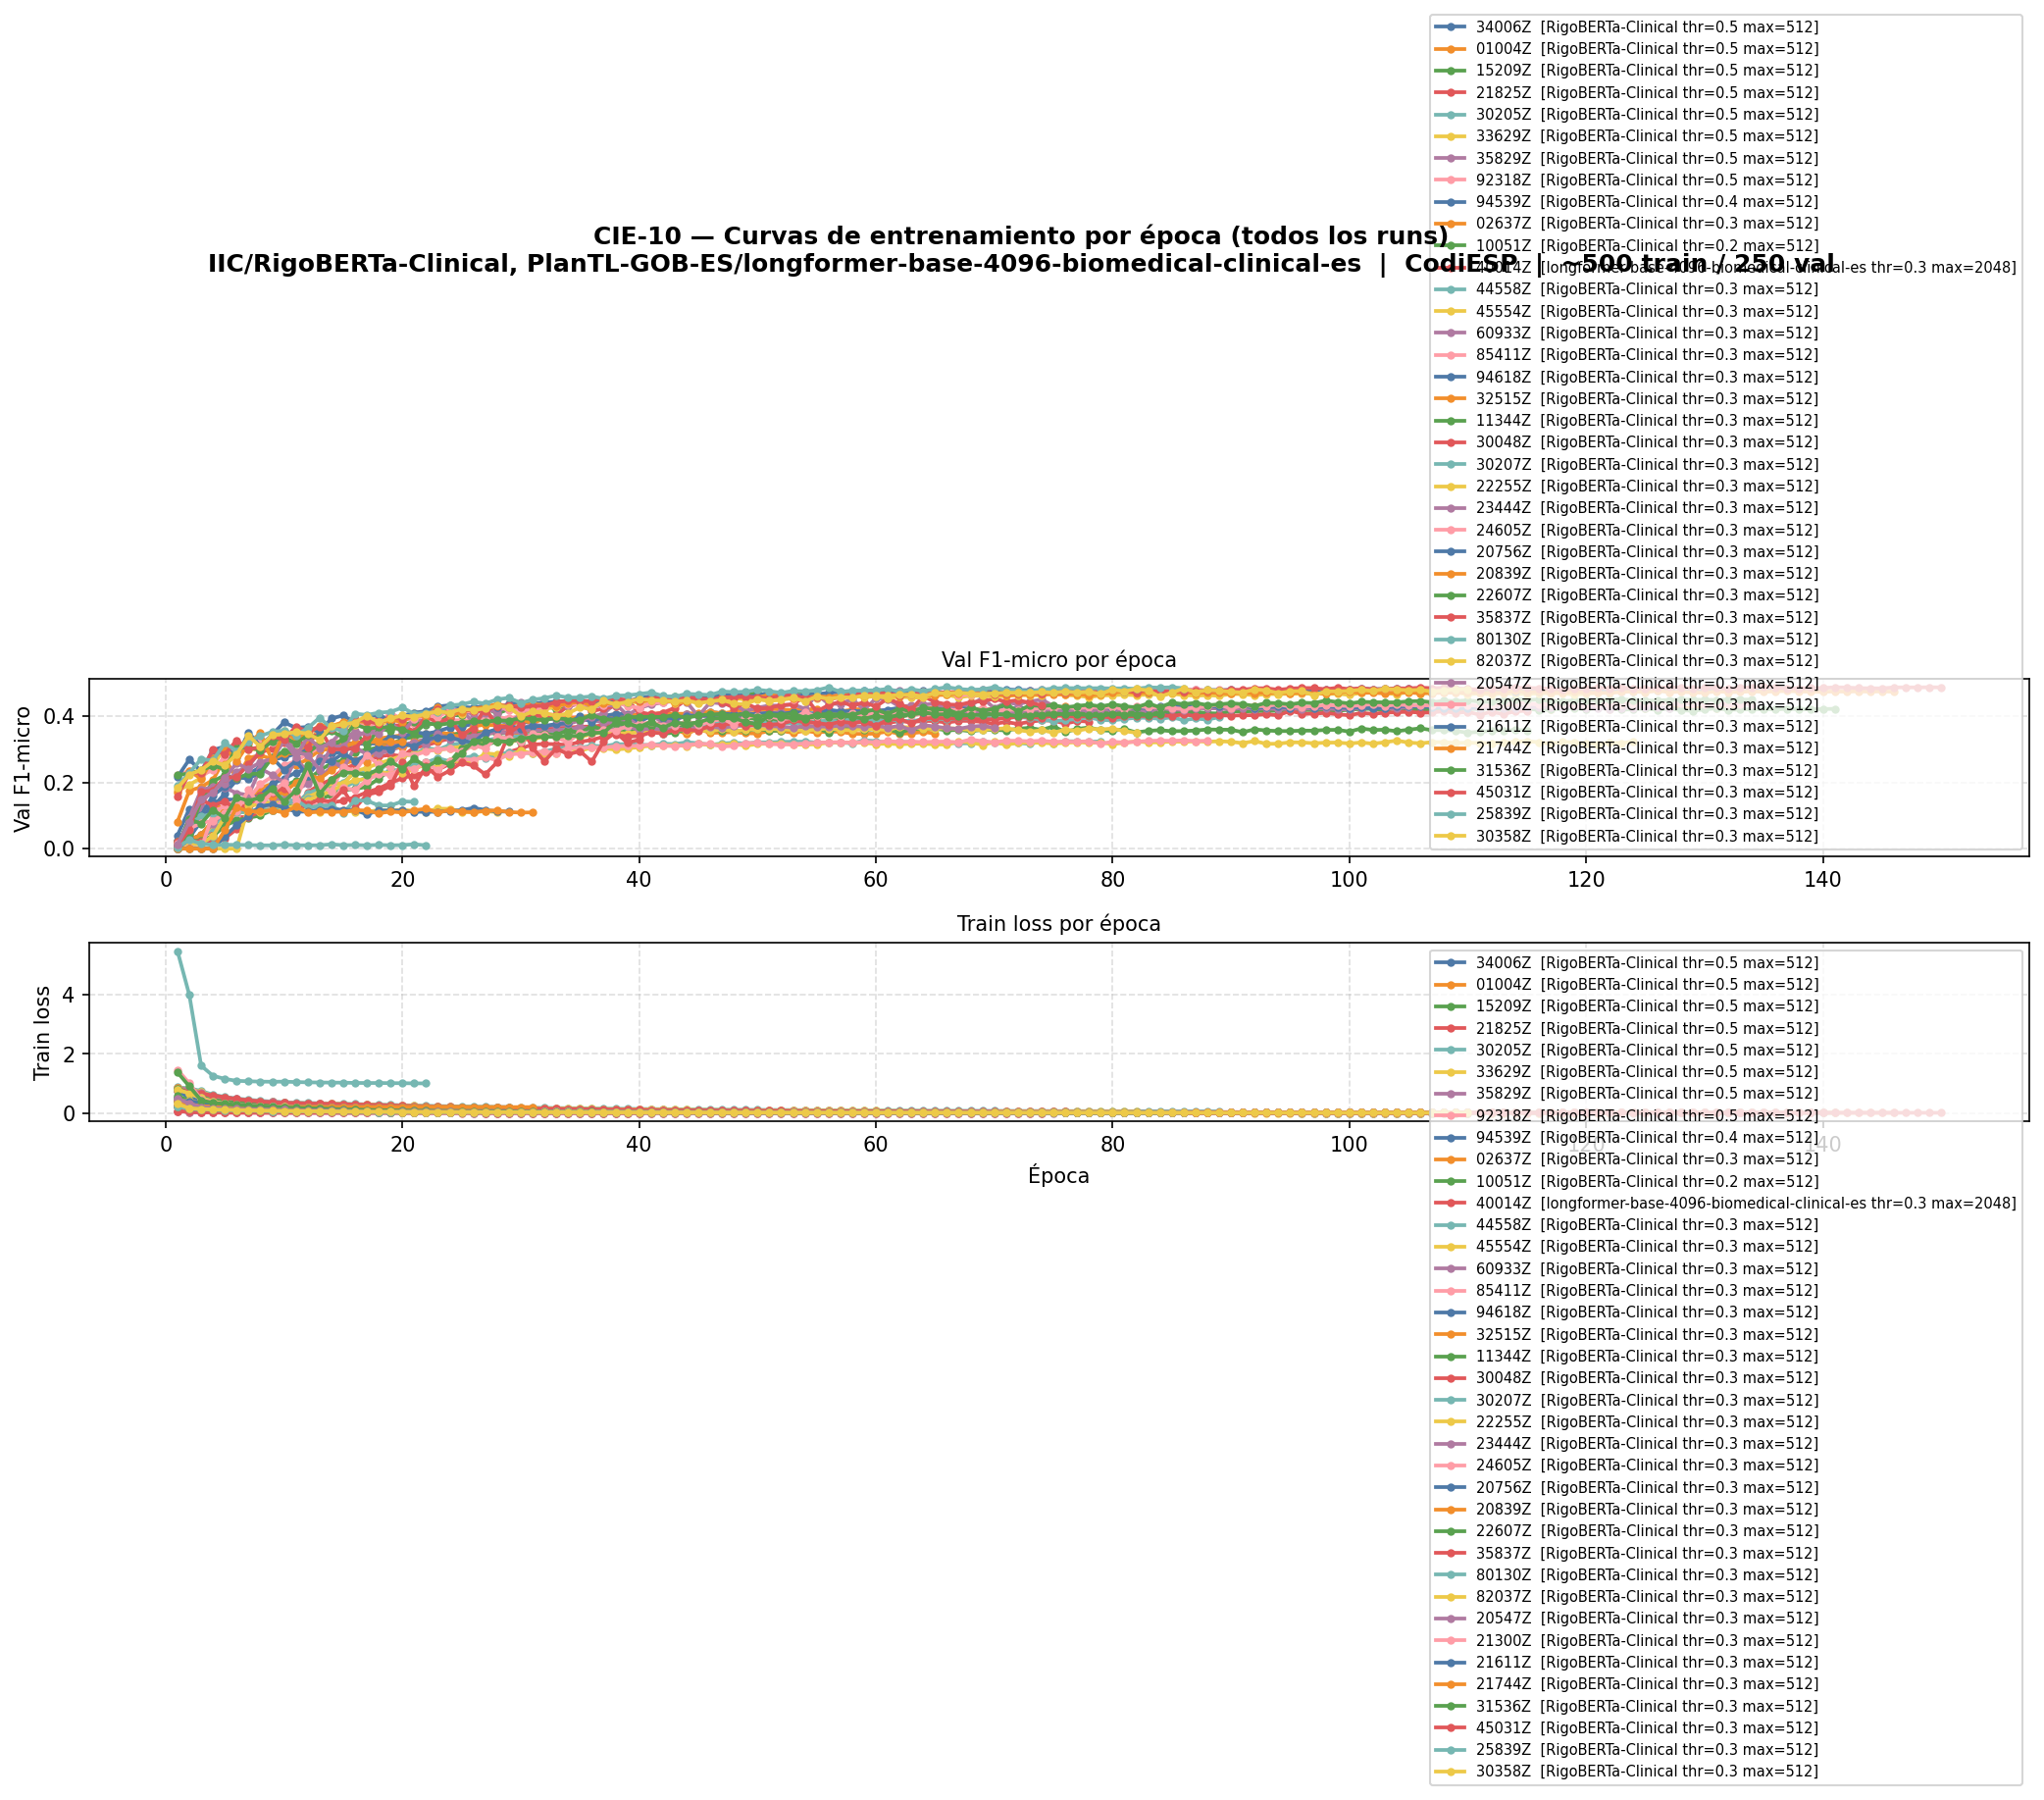
\includegraphics[width=\textwidth]{figs/all_epochs_graph}
\caption{Curvas de entrenamiento: F1-micro de validación y pérdida de entrenamiento por época.}
\label{fig:epochs-graph}
\end{figure}

\section{Artefactos del modelo}

Los artefactos del modelo desplegado en producción se encuentran en \texttt{ai\_engine/model/}:

\begin{description}
    \item[\texttt{classifier.pt}] Pesos del modelo PyTorch (ejecución del paso~36).
    \item[\texttt{thresholds.json}] Umbrales por clase optimizados sobre el conjunto de validación.
    \item[\texttt{config.json}] Metadatos del modelo activo: nombre, fichero de pesos, fichero de umbrales y parámetros de inferencia.
\end{description}
 % Anexo H: Configuración y resultados del entrenamiento final
\chapter{Arquitectura de producción}
\label{cap:AnexoI}

Este anexo describe la arquitectura de despliegue del sistema: una estación de trabajo local, orquestada con Docker Compose y con Traefik como proxy inverso, publicada en Internet a través de un túnel de Cloudflare. El mismo \emph{stack} que se usa en desarrollo se despliega sin modificaciones, añadiendo únicamente la capa de enrutamiento y TLS que proporciona Traefik.

\section{Motivación y elección de infraestructura}

La elección de una máquina propia frente a proveedores cloud gestionados responde al coste. El motor de IA se beneficia de una GPU, y un nodo con acelerador en Azure o Google Cloud Platform supera los 1.000\,€/mes, cifra que ningún prototipo sin usuarios justifica. La estación de trabajo ya existía como equipo de desarrollo, de modo que alojar en ella el sistema no añade coste: es el mismo AMD Ryzen 9 7900X con una NVIDIA RTX 4080 sobre el que se han hecho todas las mediciones de este trabajo.

Que la máquina que sirve sea la misma que mide no basta para que el servicio use el acelerador, y conviene declararlo porque durante buena parte del desarrollo no lo usó. El fichero de superposición compilaba la imagen con CUDA y reservaba la tarjeta, pero no cambiaba la variable \texttt{DEVICE}, que el \texttt{Dockerfile} deja en \texttt{cpu}. El síntoma no era un error sino una lentitud aceptada: el sistema funcionaba y respondía, solo que el ciclo completo costaba 11\,s en lugar de medio segundo. Al corregirlo aparecieron dos fallos más que solo se manifiestan con la tarjeta visible, ambos descritos en el capítulo de desarrollo.

Usando la GPU, que es como se sirve hoy el motor de IA en esta máquina, el ciclo completo por informe baja a \textbf{0,53\,s} (0,017\,s en proponer y 0,51\,s en justificar) frente a los \textbf{16,5\,s} que costaría el mismo ciclo en CPU (0,331\,s y 16,2\,s respectivamente; Tabla~\ref{tab:latencia} del capítulo de desarrollo, que detalla cómo se mide cada cifra). Tener GPU no elimina la necesidad de desacoplar la atribución en una petición aparte: el modo CPU sigue siendo un escenario de despliegue soportado (Anexo~\ref{cap:AnexoK}), por ejemplo si la tarjeta no estuviera disponible, y ahí justificar un código sigue costando dos órdenes de magnitud más que proponerlo.

La simplicidad operativa es el segundo factor. No hay clúster que gestionar, ni \emph{control plane}, ni herramientas adicionales: \texttt{provision.sh} + \texttt{make setup} + \texttt{make deploy} y el sistema está en funcionamiento. El número de piezas que pueden fallar es mínimo.

Publicar una máquina local en Internet exigiría abrir puertos en el router, disponer de dirección estable y exponer la superficie de ataque del propio equipo. Un túnel de Cloudflare evita las tres cosas: el contenedor \texttt{cloudflared} abre una conexión saliente hacia la red de Cloudflare y el tráfico entra por ahí, sin que ningún puerto del equipo quede accesible desde fuera.

La portabilidad futura no se compromete: todos los servicios están dockerizados y las únicas piezas específicas del entorno son los ficheros de superposición de Docker Compose (\texttt{docker-compose.prod.yml}, \texttt{docker-compose.gpu.yml} y \texttt{docker-compose-proxy.yml}) junto con el script \texttt{provision.sh}. Si el volumen de usuarios llegara a justificar el coste, la migración a un servidor alojado o a un clúster cloud no requiere cambios en ningún componente de la aplicación. Hoy ese coste no está justificado: el sistema es un prototipo de demostración sin usuarios reales, y pagar por una infraestructura dimensionada para una carga que no existe sería gasto sin contrapartida.

\section{Infraestructura}

El servidor es la estación de trabajo de desarrollo (AMD Ryzen 9 7900X, NVIDIA RTX 4080), publicada en Internet mediante un túnel de Cloudflare. La pila de software se compone de:

\begin{itemize}
    \item \textbf{Sistema operativo}: Ubuntu LTS.
    \item \textbf{Docker Engine}: gestor de contenedores y red.
    \item \textbf{Docker Compose}: orquestación de los servicios de la aplicación.
    \item \textbf{Traefik v3}: proxy inverso, terminación TLS y enrutamiento por dominio.
    \item \textbf{cloudflared}: túnel saliente que publica los servicios sin abrir puertos entrantes.
\end{itemize}

La Figura~\ref{fig:infra-prod} resume la topología resultante, desde la entrada del tráfico por Cloudflare hasta los contenedores de la aplicación.

\begin{figure}[ht]
\centering
\resizebox{0.85\textwidth}{!}{
\begin{tikzpicture}[
  every node/.style={font=\small\sffamily},
  ext/.style={draw=palered!80, fill=palered!10, thick, rectangle, rounded corners=3pt,
              minimum width=3.0cm, minimum height=0.95cm, align=center},
  prox/.style={draw=ocre!80, fill=ocre!15, thick, rectangle, rounded corners=3pt,
               minimum width=8.2cm, minimum height=0.9cm, align=center},
  svc/.style={draw=aquaESI!80, fill=aquaESI!15, thick, rectangle, rounded corners=3pt,
              minimum width=2.4cm, minimum height=0.95cm, align=center},
  dbc/.style={draw=turquesa!80, fill=turquesa!15, thick, cylinder, shape border rotate=90,
              aspect=0.22, minimum width=2.2cm, minimum height=1.0cm, align=center},
  arr/.style={->, >=Stealth, thick},
]
\node[ext] (user) at (0,3.4) {Usuario};
\node[ext] (cf)   at (0,2.0) {Cloudflare\\\scriptsize WAF $\cdot$ DDoS $\cdot$ TLS de borde};

\draw[rounded corners=6pt, dashed, gray!55, thick] (-4.7,-4.15) rectangle (4.7,1.15);
\node[black!70, font=\small\sffamily\bfseries] at (0,-3.9)
  {Estación de trabajo $\cdot$ Docker Compose};

\node[prox] (tk) at (0,0.2) {Traefik \scriptsize (proxy inverso)};
\node[svc] (fe) at (-3.2,-1.3) {Frontend\\\scriptsize Next.js};
\node[svc] (be) at (-0.3,-1.3) {Backend\\\scriptsize Phoenix};
\node[svc, minimum width=2.9cm] (mon) at (3.1,-1.3) {Prometheus,\\Grafana y Loki};
\node[svc] (ai) at (-1.8,-3.0) {AI Engine\\\scriptsize FastAPI (GPU)};
\node[dbc] (pg) at (1.4,-3.0) {PostgreSQL};

\draw[arr] (user) -- (cf);
\draw[arr] (cf) -- (tk);
\draw[arr] (tk) -- (fe);
\draw[arr] (tk) -- (be);
\draw[arr] (be) -- (ai);
\draw[arr] (be) -- (pg);
\draw[arr, black!70, dashed] (mon) -- (be);
\end{tikzpicture}
}
\caption{Arquitectura de despliegue: el tráfico entra por Cloudflare (WAF, DDoS y TLS de borde) y baja por el túnel hasta la estación de trabajo, donde Traefik actúa de proxy inverso con TLS de Let's Encrypt y enruta a los servicios Docker (frontend, backend, motor de IA con GPU y PostgreSQL), monitorizados con Prometheus y Grafana.}
\label{fig:infra-prod}
\end{figure}

\section{Aprovisionamiento}

El script \texttt{provision.sh} automatiza la puesta en marcha de un servidor desde cero:

\begin{lstlisting}[language=bash, caption={Pasos del script de aprovisionamiento.}, label=lst:provision-sh]
# 1. Crear usuario `app` sin privilegios
# 2. Generar clave SSH ed25519 y añadirla a GitHub (pausa interactiva)
# 3. Instalar Docker Engine via get.docker.com
# 4. Instalar y configurar fail2ban (jails sshd y traefik-auth)
# 5. Clonar el repositorio en /home/app/CIE-10
# 6. Copiar .env.example -> .env (para edición manual de credenciales)
\end{lstlisting}

Tras ejecutar \texttt{provision.sh}, el operador edita el fichero \texttt{.env} con las credenciales reales (base de datos, SMTP, claves de aplicación, token de HuggingFace) y lanza el despliegue.

\section{Flujo de despliegue}

El proceso completo desde un servidor recién aprovisionado se reduce a tres pasos:

\begin{enumerate}
    \item \textbf{Aprovisionamiento del servidor}: \texttt{sudo bash provision.sh} (requiere root para instalar Docker, crear el usuario \texttt{app} y configurar fail2ban).
    \item \textbf{Setup inicial} (construcción de imágenes, migraciones y seed): \texttt{make setup}
    \item \textbf{Despliegue}: \texttt{make deploy}
\end{enumerate}

\texttt{make deploy} arranca en orden: la red Docker compartida, Traefik (proxy), el \emph{stack} de monitorización (Prometheus + Grafana) y los servicios de la aplicación (base de datos, backend, frontend, motor de IA). En entorno de desarrollo el flujo es equivalente pero sin Traefik ni monitorización: \texttt{make setup up}.

\section{Proxy inverso con Traefik}

Traefik se despliega como un servicio Docker independiente definido en \texttt{docker-compose-proxy.yml}. Su configuración es declarativa: cada servicio de la aplicación expone sus rutas mediante etiquetas Docker (\emph{labels}), y Traefik las descubre automáticamente sin necesidad de recargar configuración.

\begin{lstlisting}[language=bash, caption={Fragmento de configuración de Traefik.}, label=lst:traefik-config]
# Entrypoints: HTTP (:80) redirige permanentemente a HTTPS (:443)
# Let's Encrypt: certificados TLS via HTTP challenge, renovación automática
# Red Docker: escucha en la red `clicoder` y descubre servicios por labels
# Dashboard: protegido con Basic Auth y rate-limiting
\end{lstlisting}

Los certificados TLS se obtienen y renuevan automáticamente mediante Let's Encrypt (HTTP challenge). El dominio \texttt{clicoder.app} está registrado y apunta al servidor de producción.

\section{Protección con Cloudflare}

El dominio \texttt{clicoder.app} está configurado con el proxy de Cloudflare activado. El tráfico de los usuarios pasa primero por la red de Cloudflare antes de llegar al servicio, lo que aporta tres capas de protección sin coste adicional:

\begin{itemize}
    \item \textbf{Protección frente a bots y \emph{scraping}}: Cloudflare filtra el tráfico automatizado malicioso y bloquea los agentes de rastreo no autorizados antes de que alcancen el servidor.
    \item \textbf{Mitigación de ataques de denegación de servicio} (DDoS): la red distribuida de Cloudflare absorbe el tráfico volumétrico sin que los contenedores lleguen a recibir la carga.
    \item \textbf{Ocultación de la IP del servidor}: la dirección IP real del servidor no es visible desde el exterior; los atacantes solo conocen las IPs de Cloudflare, lo que reduce la superficie de ataque directa.
\end{itemize}

Esta capa de protección es complementaria a Traefik: Cloudflare actúa en el borde de la red, antes de que el paquete llegue al servidor, mientras que Traefik gestiona el enrutamiento y TLS una vez que el tráfico ya ha pasado por el proxy.

\subsection{Cloudflare Tunnel}

Como alternativa al proxy DNS, el despliegue admite un \textbf{túnel de Cloudflare} (\texttt{cloudflared}), que se activa con \texttt{make start-tunnel} y requiere un \texttt{CLOUDFLARE\_TUNNEL\_TOKEN} en el fichero \texttt{.env}. El contenedor establece una conexión \emph{saliente} y persistente hacia la red de Cloudflare, de modo que el tráfico entrante se entrega a través de ese túnel.

La diferencia operativa es relevante: con el túnel el servidor \textbf{no necesita exponer los puertos 80 y 443}, por lo que la ocultación de la dirección IP deja de depender de la configuración del DNS y pasa a ser una propiedad estructural del despliegue. Reduce así la superficie de ataque directa sobre el servicio. El mismo fichero \texttt{docker-compose-proxy.yml} define además un servicio de \emph{página de mantenimiento} (nginx) que permite servir un aviso estático mientras la aplicación está detenida.

\section{Protección con Fail2ban}

Cloudflare filtra el tráfico en el borde de la red, pero no actúa sobre intentos de acceso por SSH ni sobre peticiones que llegan directamente al servidor. Fail2ban cubre esta superficie residual: monitoriza los logs del sistema y de Traefik, y bloquea a nivel de \texttt{iptables} las IPs que muestran comportamiento de fuerza bruta.

La distinción respecto al \emph{rate limiting} de Traefik es relevante. El \emph{middleware} de Traefik devuelve \texttt{429 Too Many Requests}, pero la IP sigue abriendo conexiones TCP y consumiendo recursos del servidor. Fail2ban, en cambio, inserta una regla en \texttt{iptables} que descarta los paquetes antes de que lleguen a ningún servicio.

El script \texttt{provision.sh} instala y configura fail2ban con las dos \emph{jails} de la Tabla~\ref{tab:fail2ban-jails}:

\begin{table}[h]
\centering
\caption{Jails de fail2ban configurados en producción.}
\label{tab:fail2ban-jails}
\begin{tabular}{llll}
\hline
\textbf{Jail} & \textbf{Fuente de logs} & \textbf{Umbral} & \textbf{Ban} \\
\hline
\texttt{sshd}         & \texttt{/var/log/auth.log}            & 3 intentos fallidos    & 24 h \\
\texttt{traefik-auth} & \texttt{/var/log/traefik/access.log}  & 10 respuestas 401 en 5 min & 1 h  \\
\hline
\end{tabular}
\end{table}

El \emph{jail} de Traefik se apoya en que el servicio escribe los \emph{access logs} en formato JSON al fichero \texttt{/var/log/traefik/access.log}, montado como \emph{bind mount} desde el host. El filtro personalizado \texttt{traefik-auth} extrae el campo \texttt{ClientHost} de cada línea con \texttt{DownstreamStatus: 401}, lo que cubre cualquier \emph{endpoint} de autenticación del backend sin necesidad de hardcodear rutas.

\section{Copias de seguridad}

La copia de seguridad se hace con \texttt{pg\_dump} sobre las dos bases de datos que el sistema mantiene: la de la aplicación y la del registro de eventos. Volcarlas por separado no es un detalle de implementación: la segunda contiene el historial inmutable de decisiones, que es lo que sostiene el requisito de trazabilidad, de modo que una copia que solo cubriera la primera dejaría fuera precisamente lo que no se puede reconstruir.

El comando es \texttt{make db-backup}, y se programa con una entrada de \emph{cron} en el equipo anfitrión:

\begin{lstlisting}[language=bash, caption={Programacion diaria de la copia de seguridad.}, label=lst:cron-backup]
0 4 * * * cd /ruta/al/proyecto && make db-backup >> /var/log/cie10-backup.log 2>&1
\end{lstlisting}

Conviene declarar la limitación: al tratarse de una máquina única, la copia reside en el mismo equipo que los datos. Eso protege frente a un error de la aplicación o un borrado accidental, pero no frente a la pérdida del equipo. Replicarla a un almacenamiento externo queda como trabajo futuro, y es la primera pieza que habría que añadir antes de tratar datos clínicos reales.

\section{Comparativa de costes}

La Tabla~\ref{tab:local-vs-cloud} muestra la diferencia de coste entre el despliegue actual y dos alternativas cloud gestionadas: una con instancia GPU dedicada y otra íntegramente en CPU.

\begin{table}[h]
\centering
\caption{Comparativa de costes: local frente a cloud gestionado (GCP, región europea, on-demand, junio 2026).}
\label{tab:local-vs-cloud}
\begin{tabular}{llr}
\hline
\textbf{Setup} & \textbf{Descripción} & \textbf{Coste aprox.} \\
\hline
Local (actual)        & Docker Compose y túnel de Cloudflare sobre equipo propio & $\sim$330\,€/año\footnotemark[5] \\
\hline
Cloud con GPU\footnotemark[1]
                      & Nodos CPU (frontend + backend)                & $\sim$140\,€/mes \\
                      & Nodo GPU (motor de IA, 1$\times$ V100)\footnotemark[2] & $\sim$1.950\,€/mes \\
                      & Base de datos gestionada (PostgreSQL)\footnotemark[3] & $\sim$230\,€/mes \\
                      & \textbf{Total estimado}                       & \textbf{$\sim$2.320\,€/mes} \\
\hline
Cloud solo CPU        & Nodos CPU (frontend + backend)                & $\sim$140\,€/mes \\
                      & Nodo CPU para motor de IA (8\,vCPU, 30\,GB)\footnotemark[4] & $\sim$230\,€/mes \\
                      & Base de datos gestionada (PostgreSQL)\footnotemark[3] & $\sim$230\,€/mes \\
                      & \textbf{Total estimado}                       & \textbf{$\sim$600\,€/mes} \\
\hline
\end{tabular}
\end{table}
\footnotetext[1]{GCP europe-west4. Precios on-demand consultados en junio de 2026. Fuente: \url{https://cloud.google.com/compute/gpus-pricing}}
\footnotetext[2]{Instancia n1-standard-8 + 1$\times$ NVIDIA V100: \$2,55/h GPU + \$0,35/h VM $\approx$ \$2.117/mes $\approx$ 1.950\,€/mes.}
\footnotetext[3]{Cloud SQL PostgreSQL, 4\,vCPU / 16\,GB RAM, estimado para europe-west4. Fuente: \url{https://cloud.google.com/sql/pricing}}
\footnotetext[4]{Instancia n1-standard-8 (8\,vCPU, 30\,GB RAM) para alojar el modelo RigoBERTa-Clinical en CPU ($\sim$13\,GB de RAM en inferencia).}
\footnotetext[5]{Solo consumo eléctrico: el equipo ya existía como estación de desarrollo, de modo que su compra no es un coste imputable al despliegue. Estimado a partir de 250\,W medios continuos y un precio de 0{,}15\,€/kWh. El túnel de Cloudflare se usa en su plan gratuito.}

La GPU no es estrictamente necesaria para proponer códigos: el motor opera igualmente en CPU y la predicción se resuelve por debajo del segundo. Sí lo es para justificarlos sin espera, y de ahí que el diseño desacople la atribución en una petición aparte. Aun renunciando al acelerador, la opción cloud solo en CPU cuesta más de veinte veces al año lo que el despliegue actual, porque las instancias de aplicación son pequeñas pero el modelo exige un nodo con suficiente RAM ($\sim$13\,GB) para cargarse íntegramente. En ambos escenarios cloud el coste está dominado por componentes que en un único equipo se comparten sin sobrecoste. La conclusión no es que el cloud sea mala opción, sino que su coste se justifica con una carga de usuarios que este prototipo todavía no tiene.
 % Anexo I: Arquitectura de despliegue (Docker Compose + Traefik + túnel de Cloudflare)
\chapter{Tablero Kanban: listado completo de tareas}\label{cap:AnexoJ}

Este anexo recoge, en la Tabla~\ref{tab:kanban}, el listado completo de tareas que componen el tablero Kanban del proyecto, organizadas por épica. Los identificadores de tarea (\texttt{T-XX}) son los empleados en el tablero durante el desarrollo para referenciar cada ítem. La última columna recoge la prioridad de atención dentro de cada épica o, en su caso, el estado de exclusión: \textbf{Alta} (bloquea el avance de otras tareas), \textbf{Media} (necesaria pero no bloqueante), \textbf{Baja} (mejora o calidad sin impacto crítico en el camino principal) y \textbf{Descartada} (identificada durante el desarrollo pero excluida explícitamente del alcance del proyecto).

\begin{center}
\small
\begin{longtable}{llp{7cm}c}
\caption{Listado completo de tareas del tablero Kanban con su prioridad o estado, agrupadas por épica.}\label{tab:kanban}\\
\hline
\textbf{ID} & \textbf{Épica} & \textbf{Tarea} & \textbf{Prioridad / estado} \\
\hline
\endfirsthead
\hline
\textbf{ID} & \textbf{Épica} & \textbf{Tarea} & \textbf{Prioridad / estado} \\
\hline
\endhead
\hline
\endfoot

T-01 & Datos & Descarga del corpus CodiEsp (diagnósticos, procedimientos y variante extendida) & Alta \\
T-02 & Datos & Análisis estadístico del corpus: distribución de longitudes, frecuencia de códigos y desequilibrio de clases & Alta \\
T-03 & Datos & Desarrollo del script de \emph{scraping} sobre el portal eCIE-maps para obtener el catálogo CIE-10-ES & Alta \\
T-04 & Datos & Análisis estadístico del catálogo CIE-10-ES: cobertura, distribución por capítulos y vocabulario & Media \\
T-05 & Datos & Generación de los ficheros CSV de entrenamiento, validación y test & Alta \\
T-48 & Datos & Aumentación del corpus CodiEsp mediante retrotraducción con Azure Translator (F0, nivel gratuito) usando tres pivotes (EN, DE, FR), cuadruplicando el corpus de 500 a 2.000 documentos (evaluada y finalmente descartada por no superar la referencia de 500 documentos; véase el Anexo~\ref{cap:AnexoL}) & Media \\
\hline
T-06 & Modelo & Comparativa de modelos base candidatos (IIC/RigoBERTa-Clinical, mmBERT, BETO) & Alta \\
T-07 & Modelo & Implementación del clasificador plano multilabel basado en BERT & Alta \\
T-08 & Modelo & Configuración del pipeline de entrenamiento (BCE con ponderación, AdamW, \emph{scheduler}) & Alta \\
T-09 & Modelo & Implementación del clasificador de diccionario como \emph{baseline} & Media \\
T-10 & Modelo & Entrenamiento y selección del mejor \emph{checkpoint} por F1-micro en validación & Alta \\
T-11 & Modelo & Evaluación sobre el conjunto de test con métricas de precisión, \emph{recall} y F1 & Media \\
T-46 & Modelo & Activación de FlashAttention~2 como implementación eficiente del mecanismo de atención: integrada en la imagen base GPU (\texttt{cie10-ml-base}) con fallback a SDPA; activa en todas las ejecuciones de entrenamiento & Media \\
\hline
T-12 & AI Engine & Implementación del servicio FastAPI con entorno virtualizado & Alta \\
T-13 & AI Engine & Endpoint \texttt{POST /predict} y \texttt{GET /} & Alta \\
T-14 & AI Engine & Desarrollo del servicio \emph{mock} para entornos CI y desarrollo sin GPU & Alta \\
T-15 & AI Engine & Dockerización con imagen base optimizada para PyTorch & Media \\
\hline
T-16 & Backend & Configuración del entorno y herramientas de calidad (linting, análisis estático) & Alta \\
T-17 & Backend & Sistema de autenticación: registro, confirmación por email e inicio de sesión & Alta \\
T-18 & Backend & Arquitectura CQRS/Event Sourcing con Commanded y PostgreSQL como \emph{event store} & Alta \\
T-19 & Backend & Canal WebSocket para comunicación en tiempo real con el frontend & Alta \\
T-20 & Backend & Pipeline de análisis: recepción del informe, llamada al AI Engine y almacenamiento & Alta \\
T-21 & Backend & Soporte de internacionalización (i18n) en cinco idiomas & Media \\
T-22 & Backend & Suite de pruebas con ExUnit e informe de cobertura con excoveralls & Media \\
T-23 & Backend & Dockerización del entorno de desarrollo, pruebas y producción & Media \\
\hline
T-24 & Frontend & Página de autenticación con formularios de registro e inicio de sesión & Alta \\
T-25 & Frontend & Interfaz de chat con renderizado de tarjetas tipadas (resumen y códigos) & Alta \\
T-26 & Frontend & Panel lateral con historial de análisis y controles de sesión & Alta \\
T-27 & Frontend & Componentes de validación y rechazo de códigos predichos con motivo & Alta \\
T-28 & Frontend & Selector de idioma y carga de traducciones desde el backend & Media \\
T-29 & Frontend & Configuración centralizada de URLs mediante variables de entorno & Baja \\
T-30 & Frontend & Dockerización del entorno de desarrollo, pruebas y producción & Media \\
\hline
T-31 & Infraestructura & Configuración de Docker Compose para todos los servicios & Alta \\
T-32 & Infraestructura & Makefile con \emph{targets} para el ciclo de vida completo del proyecto & Media \\
T-33 & Infraestructura & Configuración de commitlint y Husky para validación de mensajes de commit & Baja \\
T-34 & Infraestructura & Workflow de GitHub Actions para integración continua & Media \\
T-35 & Infraestructura & Dockerización del entorno de entrenamiento con soporte CPU y GPU & Alta \\
T-36 & Infraestructura & Despliegue con Docker Compose y Traefik como proxy inverso (TLS automático de Let's Encrypt), publicado mediante un túnel de Cloudflare & Media \\
T-37 & Infraestructura & Monitorización con Prometheus y Grafana: el backend expone métricas de latencia HTTP, queries Ecto y VM BEAM en \texttt{:9568/metrics} mediante \texttt{telemetry\_metrics\_prometheus}; Prometheus scrapea todos los servicios y Grafana los visualiza con datasource provisionado automáticamente & Baja \\
T-38 & Infraestructura & Gestión de errores y excepciones con Sentry: captura de excepciones HTTP mediante \texttt{Sentry.PlugCapture} en el endpoint Phoenix, captura de crashes OTP (GenServer, comandos Commanded) mediante \texttt{Sentry.LoggerHandler}, con stacktrace completo y etiqueta de entorno configurada vía \texttt{SENTRY\_DSN} & Baja \\
T-47 & Infraestructura & Configuración del servidor de email en producción con registros SPF, DKIM y política DMARC para garantizar la entregabilidad y autenticidad de los emails transaccionales & Media \\
\hline
T-39 & Modelo & Bucle de aprendizaje activo: reentrenamiento incremental con códigos validados por el codificador & Descartada \\
T-40 & Modelo & Soporte de codificación de procedimientos CIE-10-ES (ICD-10-PCS) además de diagnósticos & Descartada \\
T-41 & Backend & Control de acceso por roles: administrador, codificador clínico y supervisor & Descartada \\
T-42 & Backend & Integración con el estándar HL7 FHIR para importación de informes desde sistemas HIS & Descartada \\
T-43 & Backend & Autenticación federada mediante OAuth~2.0 / SSO hospitalario & Descartada \\
T-44 & Frontend & Procesamiento por lotes: envío y codificación de múltiples informes de forma simultánea & Descartada \\
T-45 & Modelo & Motor de codificación por búsqueda inversa: indexación del catálogo CIE-10-ES con BM25/TF-IDF y recuperación de códigos por similitud léxica con el informe & Descartada \\
\hline
\end{longtable}
\end{center}
 % Anexo J: Tablero Kanban, listado completo de tareas
\chapter{Guía de arranque del sistema}
\label{cap:AnexoK}

Este anexo describe los pasos necesarios para poner en marcha el sistema en un entorno de desarrollo local. Toda la infraestructura se gestiona mediante Docker Compose y un \texttt{Makefile} que centraliza los comandos habituales.

\section{Requisitos previos}

\begin{itemize}
 \item \textbf{Docker} 24 o superior con el plugin \texttt{docker compose} (v2).
 \item \textbf{GNU Make}.
 \item \textbf{Git}.
 \item \textit{Opcional, modo GPU:} controlador NVIDIA y \texttt{nvidia-container-toolkit} instalados en el sistema anfitrión.
\end{itemize}

\section{Configuración del entorno}

Antes de arrancar por primera vez es necesario crear el fichero de variables de entorno a partir de la plantilla incluida en el repositorio:

\begin{lstlisting}[language=bash]
cp .env.example .env
\end{lstlisting}

Los valores por defecto son válidos para un entorno local de desarrollo. El catálogo completo de variables, con sus valores por defecto y el servicio que las consume, se recoge en el Anexo~\ref{cap:AnexoB} (Tabla~\ref{tab:envvars}).

\section{Primera puesta en marcha}

La primera vez es necesario ejecutar dos comandos en orden. El primero prepara el entorno: detiene los servicios previos y elimina sus volúmenes (incluida la base de datos), construye las imágenes Docker, descarga el modelo desde Hugging Face (\texttt{make model-download}, que usa \texttt{HUGGING\_FACE\_HUB\_TOKEN} del \texttt{.env}), crea y migra las bases de datos y carga los datos iniciales y el catálogo CIE-10:

\begin{lstlisting}[language=bash]
make setup
\end{lstlisting}

Este proceso puede tardar varios minutos la primera vez, principalmente por la descarga de imágenes base y la compilación de dependencias Elixir. \textbf{No levanta los servicios}; una vez completado, hay que arrancarlos explícitamente:

\begin{lstlisting}[language=bash]
make up
\end{lstlisting}

\section{Arranque y parada habituales}

A partir de la segunda vez, el ciclo de trabajo diario se reduce a dos comandos (\texttt{make up} detecta la GPU con \texttt{nvidia-smi} y, si no hay, arranca el motor de IA en CPU):

\begin{lstlisting}[language=bash]
make up # Levanta todos los servicios en segundo plano
make down # Detiene todos los servicios
\end{lstlisting}

Tras ejecutar \texttt{make up} los servicios quedan accesibles en las siguientes URLs (tabla~\ref{tab:urls}).

\begin{table}[h]
\centering
\caption{URLs de acceso a los servicios en entorno local.}
\label{tab:urls}
\begin{tabular}{ll}
\hline
\textbf{Servicio} & \textbf{URL} \\
\hline
Frontend (Next.js) & \url{http://localhost:3000} \\
Backend API (Phoenix) & \url{http://localhost:4000} \\
Motor de IA (FastAPI) & \url{http://localhost:8000} \\
Backoffice admin (Phoenix) & \url{http://localhost:4000/admin} \\
Mailpit (bandeja SMTP, solo desarrollo) & \url{http://localhost:8025} \\
Prometheus & \url{http://localhost:9090} \\
Grafana & \url{http://localhost:3030} \\
PostgreSQL & \texttt{localhost:5432} \\
\hline
\end{tabular}
\\[4pt]
{\footnotesize Fuente: objetivo \texttt{up} del \texttt{Makefile}.}
\end{table}

\section{Modos de ejecución}

El sistema admite tres modos de ejecución en función de la disponibilidad de hardware y del estado del modelo entrenado (tabla~\ref{tab:modos}).

\begin{table}[h]
\centering
\caption{Modos de ejecución disponibles.}
\label{tab:modos}
\begin{tabular}{llP{6.2cm}}
\hline
\textbf{Modo} & \textbf{Comando} & \textbf{Requisito} \\
\hline
GPU & \texttt{make up} (GPU detectada) & GPU NVIDIA + modelo entrenado (preferente, entrenamiento/desarrollo/producción) \\
CPU & \texttt{make cpu-up} & Modelo entrenado (soporte, cuando no hay GPU disponible) \\
Mock & \texttt{make mock-up} & Ninguno (respuestas simuladas) \\
\hline
\end{tabular}
\\[4pt]
{\footnotesize Fuente: objetivos \texttt{up} (con la GPU detectada), \texttt{cpu-up} y \texttt{mock-up} del \texttt{Makefile}.}
\end{table}

Cada modo se describe a continuación:

\begin{sloppypar}
\begin{itemize}
 \item \textbf{GPU} (\texttt{make up}, con GPU detectada): requiere una GPU NVIDIA con \texttt{nvidia-container-toolkit} y un modelo previamente entrenado montado en \texttt{ai\_engine/model/}. Es el modo preferente siempre que hay GPU disponible, tanto en desarrollo como en producción (\texttt{make deploy GPU=1}, Anexo~\ref{cap:AnexoI}) y durante el entrenamiento, porque ofrece la máxima velocidad de inferencia.
 \item \textbf{CPU} (\texttt{make cpu-up}): carga el modelo real pero realiza la inferencia en CPU. Es el modo de soporte para cuando no hay GPU disponible, sea en desarrollo o en un despliegue sin acelerador (Anexo~\ref{cap:AnexoI}): proponer los códigos cuesta 0{,}331\,s por informe, aunque justificarlos sube a 16{,}2\,s, y de ahí que la atribución se sirva en una petición aparte.
 \item \textbf{Mock} (\texttt{make mock-up}): el motor de IA devuelve respuestas fijas sin cargar ningún modelo. Recomendado para desarrollo del frontend y pruebas funcionales del backend cuando no se dispone de modelo entrenado.
\end{itemize}
\end{sloppypar}

\section{Usuarios de prueba}

El comando \texttt{make setup} (a través de \texttt{mix run priv/repo/seeds.exs}) crea automáticamente el siguiente usuario administrador con la cuenta ya confirmada (tabla~\ref{tab:seeds}).

\begin{table}[h]
\centering
\caption{Usuario de prueba creado por el seed.}
\label{tab:seeds}
\begin{tabular}{llll}
\hline
\textbf{Email} & \textbf{Contraseña} & \textbf{Username} & \textbf{Rol} \\
\hline
\texttt{myadminuser@clicoder.app} & \texttt{password123!} & \texttt{admin} & Administrador \\
\hline
\end{tabular}
\\[4pt]
{\footnotesize Fuente: \texttt{backend/\allowbreak{}priv/\allowbreak{}repo/\allowbreak{}seeds.exs}.}
\end{table}

El correo y la contraseña del administrador son configurables mediante las variables de entorno \texttt{SEED\_ADMIN\_EMAIL} y \texttt{SEED\_ADMIN\_PASSWORD} (los valores de la tabla son los predeterminados). El usuario administrador tiene acceso al backoffice en \url{http://localhost:4000/admin}.

\section{Consulta de logs}

Para inspeccionar la salida de cualquier servicio en tiempo real:

\begin{lstlisting}[language=bash]
make logs # Menú interactivo para seleccionar el servicio
\end{lstlisting}

\section{Reset de base de datos}

Si es necesario partir de un estado limpio sin reconstruir imágenes:

\begin{lstlisting}[language=bash]
make db-reset # Drop + migrate + seed
\end{lstlisting}

\section{Motor de IA: diccionario y entrenamiento}

El motor de IA opera en dos modos complementarios: un clasificador neuronal basado en RigoBERTa-Clinical y un clasificador por diccionario (\emph{baseline}) basado en coincidencia de patrones. Ambos requieren pasos de preparación independientes.

\subsection{Regenerar el diccionario de términos clínicos}

El clasificador por diccionario utiliza un fichero \texttt{model/baseline\_dict.json} que mapea términos clínicos lematizados a bloques CIE-10. Este fichero se construye con tres fuentes, las que pasa el \texttt{Makefile} en \texttt{--sources clinical corpus combined}: \texttt{clinical} (términos clínicos reales extraídos de las anotaciones de la tarea~X de CodiEsp, ampliados con sinónimos léxicos), \texttt{corpus} (\emph{n}-gramas discriminativos minados de las notas de entrenamiento) y \texttt{combined}, la unión de las dos anteriores, que es el diccionario que se guarda. Las descripciones oficiales del catálogo (\texttt{diagnoses}, \texttt{procedures}, \texttt{chemicals}) existen como fuentes opcionales de \texttt{baseline\_dict.py}, pero no entran en el diccionario servido porque, medidas, empeoran el resultado. Adicionalmente, el sistema expande abreviaturas clínicas frecuentes en español (\texttt{HTA}, \texttt{DM2}, \texttt{EPOC}, \texttt{IAM}\dots) a su forma completa antes de lematizar, siguiendo la estrategia del equipo IAM ganador de CodiEsp~2020.

Es necesario regenerarlo cuando se modifica \texttt{baseline\_dict.py}, se actualizan los ficheros de datos de CodiEsp o se cambia cualquier parámetro de construcción del diccionario. El proceso lee los datos desde \texttt{/data/}, lematiza todos los términos con spaCy (el resultado se almacena en caché en \texttt{model/baseline\_cache/} para acelerar ejecuciones sucesivas) y escribe el diccionario resultante:

\begin{lstlisting}[language=bash]
make ai-baseline-dict 2>&1 | tee /tmp/dict.log
\end{lstlisting}

La primera ejecución puede tardar entre 15 y 30~minutos porque lematiza las decenas de miles de entradas del catálogo y las notas del corpus. Las ejecuciones posteriores son mucho más rápidas gracias a la caché. Al finalizar se imprime un resumen con el número de bloques CIE-10 cubiertos y los patrones generados por cada fuente.

Para comparar el rendimiento con y sin expansión de abreviaturas (útil para medir el impacto aislado de esa mejora), se puede desactivar puntualmente:

\begin{lstlisting}[language=bash]
make ai-baseline-dict NO_ABBREVS=1 2>&1 | tee /tmp/dict_noabbrev.log
\end{lstlisting}

\subsection{Entrenar el clasificador neuronal}

El clasificador neuronal se entrena con \texttt{train.py} sobre el corpus CodiEsp. El proceso descarga el modelo base desde Hugging Face (requiere \texttt{HF\_TOKEN} en \texttt{.env}), ajusta mediante \emph{fine-tuning} el \emph{encoder} RigoBERTa-Clinical con una cabeza de clasificación \emph{multi-label} y guarda el modelo resultante en \texttt{ai\_engine/model/}. El objetivo \texttt{make ai-train-gpu} lanza \texttt{train.py} con GPU explícita (\texttt{--device cuda}) a través del servicio \texttt{ai\_engine} y el fichero \texttt{docker-compose.gpu.yml}. Exige que la imagen del servicio se haya construido con soporte CUDA (\texttt{make build-ai GPU=1}): con una imagen construida solo para CPU falla con «Torch not compiled with CUDA enabled». En el equipo de desarrollo el entrenamiento se lanzó con \texttt{train.py} directamente sobre otra imagen que ya incluye PyTorch con CUDA (\texttt{cie-10-training}). Ejecutado sin variables usa los valores por defecto del \texttt{Makefile} (\texttt{MAX\_LENGTH=1024}, \texttt{LR=5e-6}, \texttt{DROPOUT=0.1}, \texttt{WEIGHT\_DECAY=0.01}, \texttt{FREEZE\_LAYERS=0}, \texttt{EPOCHS=20}), que \textbf{no} reproducen el modelo servido. Para reproducirlo hay que pasar todos los hiperparámetros de la ejecución \texttt{20260921T091919Z} registrada en \texttt{training\_runs.csv}:

\begin{lstlisting}[language=bash, breaklines=true, breakatwhitespace=false]
make ai-train-gpu MAX_LENGTH=512 BATCH_SIZE=8 GRAD_ACCUM=4 \
  THRESHOLD=0.3 LR=1e-4 WARMUP_RATIO=0.1 WEIGHT_DECAY=0.1 \
  DROPOUT=0.3 FREEZE_LAYERS=20 EPOCHS=150 PATIENCE=20 \
  FULL_CODES=1 LABEL_SMOOTHING=0.1 LR_SCHEDULE=plateau \
  UNFREEZE_EVERY=30 UNFREEZE_LAYERS=4 UNFREEZE_LR_RATIO=0.1 \
  PRETRAIN_EPOCHS=10 LAMBDA_HIER=0.5 SELECT_METRIC=map_macro \
  RANK_LOSS_WEIGHT=0.1 2>&1 | tee /tmp/train.log
\end{lstlisting}

El preentrenamiento con los CSV de la tarea X de CodiEsp es opcional y se activa con \texttt{PRETRAIN\_TASKX=<ruta>}; el comando anterior no lo usa. El resto de parámetros (\texttt{POS\_WEIGHT\_CAP=10}, \texttt{CHUNK\_OVERLAP=64}, \texttt{ASL\_CLIP=0.05}) coinciden con los valores por defecto del \texttt{Makefile} y de \texttt{train.py} (\texttt{ASL\_CLIP} solo está definido en este último); la ejecución original no fijó semilla, por lo que una repetición no reproduce las métricas al decimal. Este mismo comando, con las variables adicionales que se indiquen (por ejemplo \texttt{TRAIN\_FILE}), es el que se toma como base en el Anexo~\ref{cap:AnexoL}.

Cada ejecución guarda un \emph{checkpoint} con el mejor valor de validación de la métrica de selección (\texttt{SELECT\_METRIC}; el comando anterior usa \texttt{map\_macro}), los umbrales por clase optimizados y un registro de métricas por época en \texttt{model/training\_runs.csv}. La ejecución del modelo servido duró 1.409~s (unos 23,5~minutos) en la RTX 4080, y la más larga de las 58 ejecuciones registradas sobre 1.767 códigos, 1,7~horas (columna \texttt{total\_seconds} de \texttt{training\_runs.csv}).

\section{Monitorización con Prometheus y Grafana}

El sistema incluye una pila de observabilidad compuesta por Prometheus y Grafana, que en desarrollo se levanta con \texttt{make start-monitoring-dev} (\texttt{make up} no la arranca, aunque muestra sus URLs).

\subsection{URLs y credenciales}

Las URLs y credenciales de acceso están en la Tabla~\ref{tab:monitoring-urls}.

\begin{table}[h]
\centering
\caption{Acceso a las herramientas de monitorización en entorno local.}
\label{tab:monitoring-urls}
\begin{tabular}{lll}
\hline
\textbf{Herramienta} & \textbf{URL} & \textbf{Credenciales} \\
\hline
Prometheus & \url{http://localhost:9090} & Sin autenticación \\
Grafana & \url{http://localhost:3030} & \texttt{admin} / \texttt{GRAFANA\_PASSWORD} \\
\hline
\end{tabular}
\\[4pt]
{\footnotesize Fuente: \texttt{docker-compose.\allowbreak{}monitoring.\allowbreak{}dev.yml}.}
\end{table}

La contraseña de Grafana se configura mediante la variable \texttt{GRAFANA\_PASSWORD} del fichero \texttt{.env} (valor por defecto: \texttt{changeme}). La fuente de datos de Prometheus queda provisionada automáticamente al arrancar: no es necesario configurarla manualmente en la interfaz de Grafana.

\subsection{Métricas expuestas}

Prometheus recoge métricas de ocho tareas de recogida (\emph{jobs}) con un intervalo de muestreo de 15 segundos (tabla~\ref{tab:prometheus-jobs}).

\begin{table}[h]
\centering
\caption{Tareas de recogida (\emph{jobs}) configuradas en Prometheus.}
\label{tab:prometheus-jobs}
\begin{tabular}{llP{6.2cm}}
\hline
\textbf{Job} & \textbf{Endpoint} & \textbf{Métricas principales} \\
\hline
\texttt{backend} & \texttt{:9568/metrics} & Latencia HTTP (Phoenix), tiempos de consulta Ecto, memoria BEAM, colas de planificadores \\
\texttt{ai\_engine} & \texttt{:8000/metrics} & Latencia de inferencia, peticiones totales, estado del modelo \\
\texttt{prometheus} & \texttt{:9090/metrics} & Métricas internas de Prometheus \\
\texttt{cadvisor} & \texttt{:8080/metrics} & CPU, memoria, red y disco por contenedor \\
\texttt{node\_exporter} & \texttt{:9100/metrics} & Métricas del host: CPU, RAM, disco y carga \\
\texttt{traefik} & \texttt{:8082/metrics} & Peticiones, códigos de estado y latencia del proxy inverso \\
\texttt{cloudflared} & \texttt{:20241/metrics} & Estado y tráfico del túnel de Cloudflare \\
\texttt{blackbox} & \texttt{:9115/probe} & Sondas de disponibilidad HTTP de los servicios públicos \\
\hline
\end{tabular}
\\[4pt]
{\footnotesize Fuente: \texttt{docker/\allowbreak{}prometheus/\allowbreak{}prometheus.yml}.}
\end{table}

El backend Elixir utiliza \texttt{telemetry\_metrics\_prometheus} para exponer las métricas en el puerto \texttt{9568}. Las métricas de VM BEAM configuradas son \texttt{vm.memory.total} (memoria total del runtime) y \texttt{vm.total\_run\_queue\_lengths} (longitud de las colas de planificadores de CPU y de E/S), útiles para detectar saturación en el procesamiento concurrente de WebSockets. El motor de IA expone las suyas en el endpoint \texttt{/metrics} del puerto \texttt{8000} mediante \texttt{prometheus\_fastapi\_instrumentator} (métricas HTTP automáticas) más dos métricas propias: \texttt{cie10\_inference\_duration\_seconds} (histograma de latencia de inferencia) y los indicadores (\emph{gauges}) \texttt{cie10\_model\_loaded} y \texttt{cie10\_dict\_loaded} (estado de carga del modelo BERT y del clasificador de diccionario).

\subsection{Retención de datos}

Prometheus almacena los datos de series temporales durante \textbf{15 días} (configurado con \texttt{--storage.tsdb.retention.time=15d}). Los datos persisten entre reinicios del contenedor gracias al volumen Docker \texttt{prometheus\_data}. Los paneles de Grafana persisten en el volumen \texttt{grafana\_data}.

\subsection{Exploración de métricas}

Para explorar las métricas disponibles sin necesidad de construir un panel en Grafana, se puede usar directamente la interfaz web de Prometheus en \url{http://localhost:9090/graph}. Ejemplos de consultas PromQL útiles:

\begin{lstlisting}[language=bash]
# Latencia de inferencia del motor de IA (percentil 95)
histogram_quantile(0.95, rate(cie10_inference_duration_seconds_bucket[5m]))

# Estado de carga del modelo BERT (1 = cargado, 0 = no cargado)
cie10_model_loaded

# Memoria total de la VM BEAM en kilobytes
vm_memory_total_kilobytes

# Longitud de la cola de planificadores de CPU del runtime Elixir
vm_total_run_queue_lengths_cpu
\end{lstlisting}
 % Anexo K: Guía de arranque del sistema
\chapter{Aumentación de datos mediante retrotraducción}
\label{cap:AnexoL}

Este anexo describe la técnica de \emph{back-translation} (retrotraducción) aplicada al corpus CodiEsp para paliar la escasez de datos de entrenamiento, la motivación estadística que la justifica, el servicio externo empleado y los comandos necesarios para reproducirla.

%%%%%%%%%%%%%%%%%%%%%%%%%%%%%%%%%%%%%%%%%%%%%%%%%%%%%%%%%%%%%%%%%%%%%%%%%%%
\section{Motivación: el problema de la escasez de datos}
%%%%%%%%%%%%%%%%%%%%%%%%%%%%%%%%%%%%%%%%%%%%%%%%%%%%%%%%%%%%%%%%%%%%%%%%%%%

El clasificador CIE-10 del proyecto debe asignar etiquetas de un vocabulario de \textbf{1.767 códigos} a notas clínicas en español. El conjunto de entrenamiento de CodiEsp cuenta únicamente con \textbf{500 documentos}. La ratio documentos/clases es de $\approx 0{,}28$, lo que significa que la mayoría de códigos aparece en muy pocas notas de entrenamiento.

Esta situación genera dos patologías complementarias:

\begin{itemize}
  \item \textbf{Subajuste por clase minoritaria.} Los códigos que aparecen en dos o tres documentos no proporcionan señal estadística suficiente para que el modelo aprenda sus representaciones.
  \item \textbf{Sobreajuste global.} Con 500 ejemplos y un \emph{encoder} de 24 capas ($\sim$600\,M de parámetros), el modelo tiende a memorizar el corpus en lugar de generalizar.
\end{itemize}

La técnica habitual para abordar la escasez de datos en NLP cuando no se dispone de más datos anotados es la \textbf{aumentación de datos}: generar nuevas muestras sintéticas que preserven la etiqueta original pero aporten variedad léxica y sintáctica.

%%%%%%%%%%%%%%%%%%%%%%%%%%%%%%%%%%%%%%%%%%%%%%%%%%%%%%%%%%%%%%%%%%%%%%%%%%%
\section{Back-translation como aumentación}
%%%%%%%%%%%%%%%%%%%%%%%%%%%%%%%%%%%%%%%%%%%%%%%%%%%%%%%%%%%%%%%%%%%%%%%%%%%

La retrotraducción es el método de aumentación más consolidado en NLP~\cite{sennrich2016improving}. El procedimiento es:

\begin{enumerate}
  \item Traducir el texto original del español a un idioma pivote (p.~ej., inglés).
  \item Traducir el resultado de vuelta al español.
\end{enumerate}

El texto obtenido es semánticamente equivalente al original, pero con diferente elección de palabras, orden de constituyentes y estructuras sintácticas. Las etiquetas CIE-10 permanecen inalteradas porque la semántica clínica se conserva a través del pivote.

\subsection{Por qué funciona}

Desde la perspectiva del aprendizaje estadístico, añadir ejemplos retrotraducidos equivale a aplicar una forma de \emph{data augmentation} que:

\begin{itemize}
  \item \textbf{Amplía la distribución de entrada.} El modelo ve la misma nota expresada con diferentes frases, reduciendo la dependencia hacia formulaciones concretas presentes solo en el entrenamiento.
  \item \textbf{Reduce el sobreajuste.} Al cuadruplicar el tamaño del corpus con variantes distintas, la ratio parámetros/ejemplos mejora sin necesidad de reducir la capacidad del modelo.
  \item \textbf{Beneficia especialmente a las clases minoritarias.} Cada código raro que aparece en un documento pasa a aparecer también en sus tres versiones retrotraducidas, cuadruplicando la señal de entrenamiento para esa clase.
\end{itemize}

Con tres pivotes independientes (EN, DE, FR) el corpus de entrenamiento pasa de \textbf{500 a 2.000 documentos} sin coste de anotación: cada pivote añade 500 documentos retrotraducidos, sumando 1500 variantes a las 500 originales.

\subsection{Orden de los pivotes: por qué el alemán antes que el francés}

Fijado el inglés como primer pivote, quedaba decidir el orden en que incorporar los dos restantes, francés (FR) y alemán (DE). El criterio determinante es la \textbf{distancia lingüística} respecto al español: a mayor distancia, mayor recomposición sintáctica durante la retrotraducción y, por tanto, mayor variedad léxica en los ejemplos generados.

El francés es una lengua romance que comparte con el español raíces latinas y una gran parte del vocabulario médico especializado (\emph{hematoma}, \emph{diagnóstico}, \emph{paciente}…). La retrotraducción ES→FR→ES tiende a devolver textos muy similares al original, con variación limitada que apenas aporta información nueva al modelo.

El alemán, en cambio, pertenece a la rama germánica. Sus estructuras sintácticas y su formación de compuestos nominales (\emph{Herzinsuffizienz}, \emph{Bluthochdruck}) obligan al motor de traducción a reformular las oraciones de forma más profunda al retraducir al español, generando paráfrasis más diversas. Azure Translator dispone de alta calidad para el par ES$\leftrightarrow$DE en textos clínicos, comparable al par ES$\leftrightarrow$EN. Por estos motivos se incorporó \textbf{alemán (DE)} como segundo pivote y \textbf{francés (FR)} como tercero. Los tres se generaron finalmente, de modo que el corpus aumentado combina los 500 documentos originales con las 500 variantes de cada pivote; la Tabla~\ref{tab:bt-quality} confirma la previsión, con el francés como el pivote de menor variación (mediana de $0{,}0$ caracteres) y el alemán el de mayor recomposición en palabras ($+5{,}9$ de media).

%%%%%%%%%%%%%%%%%%%%%%%%%%%%%%%%%%%%%%%%%%%%%%%%%%%%%%%%%%%%%%%%%%%%%%%%%%%
\section{Servicio empleado: Azure Translator}
%%%%%%%%%%%%%%%%%%%%%%%%%%%%%%%%%%%%%%%%%%%%%%%%%%%%%%%%%%%%%%%%%%%%%%%%%%%

Se evaluaron tres alternativas para la traducción:

\begin{description}
  \item[NLLB-200 (local).] Modelo de código abierto de Meta con soporte para 200 idiomas. No requiere API ni coste externo; puede ejecutarse directamente en la GPU del entorno de entrenamiento. Desventaja: calidad inferior a los servicios cloud en textos técnicos y médicos.
  \item[DeepL.] API de alta calidad para lenguas europeas. Inconveniente: el nivel gratuito exige tarjeta de crédito como garantía, lo que lo descarta para entornos donde no se quiere vincular un método de pago.
  \item[Azure Translator.] Servicio de Microsoft Cognitive Services. El nivel \textbf{F0 (Free)} ofrece 2 millones de caracteres al mes \emph{sin tarjeta de crédito} y sin compromiso de permanencia. Cuando se supera el límite mensual el servicio bloquea las peticiones hasta el siguiente ciclo; no genera cargo adicional.
\end{description}

Se eligió Azure Translator por la combinación de calidad y ausencia de requisito de pago.

\subsection{Límites del nivel gratuito F0}

Las condiciones del nivel F0 se resumen en la Tabla~\ref{tab:azure-f0}.

\begin{table}[h]
\centering
\caption{Características del nivel gratuito F0 de Azure Translator.}
\label{tab:azure-f0}
\begin{tabular}{ll}
\hline
\textbf{Parámetro} & \textbf{Valor} \\
\hline
Caracteres por mes         & 2.000.000 \\
Tarjeta de crédito         & No requerida \\
Comportamiento al agotar   & Bloqueo hasta el siguiente mes \\
Cargo por exceso           & Ninguno \\
Idiomas disponibles        & 130+ \\
Latencia típica            & 200--800 ms por lote \\
\hline
\end{tabular}
\end{table}

El corpus CodiEsp de entrenamiento contiene \textbf{1.158.623 caracteres}. Cada pivote traduce ida y vuelta (por ejemplo ES→EN→ES), de modo que consume el doble: \textbf{2.317.246 caracteres por pivote}, ya un 16\,\% por encima del límite mensual del nivel F0. Con los tres pivotes empleados el total asciende a \textbf{6.951.738 caracteres}, equivalentes a 3,5 cuotas mensuales gratuitas. Los primeros 2.000.000 se cubrieron con la cuota mensual del nivel F0 y los 4.951.738 restantes se facturaron en modalidad de pago por uso (\emph{pay-as-you-go}) contra el \textbf{crédito gratuito de 200\,\$} que Azure concede a las cuentas nuevas, que quedó agotado al completar los tres pivotes. La aumentación no tuvo coste real, pero conviene dejar claro que \textbf{no cabe en el nivel gratuito}: quien quiera reproducirla necesita ese crédito inicial, repartir la carga entre varios recursos F0 en regiones distintas o extenderla a lo largo de varios meses.

Si el crédito gratuito se agotase antes de completar las notas, el script permite reanudar con \texttt{RESUME=1}: cuenta las filas ya escritas en el CSV de salida y retoma desde la siguiente sin retraducir nada. Como alternativa, Azure permite crear múltiples recursos Translator F0 en diferentes regiones bajo la misma cuenta, cada uno con su cuota independiente.

%%%%%%%%%%%%%%%%%%%%%%%%%%%%%%%%%%%%%%%%%%%%%%%%%%%%%%%%%%%%%%%%%%%%%%%%%%%
\section{Resultados de la aumentación}
%%%%%%%%%%%%%%%%%%%%%%%%%%%%%%%%%%%%%%%%%%%%%%%%%%%%%%%%%%%%%%%%%%%%%%%%%%%

\subsection{Distribución de códigos antes y después}

El corpus de entrenamiento de CodiEsp contiene 500 documentos con una media de \textbf{11,28 etiquetas por documento}, cubriendo los 1.767 códigos presentes en el conjunto de entrenamiento. La distribución de frecuencias es marcadamente sesgada: el \textbf{56,5\,\%} de los códigos aparece exactamente una vez, y el \textbf{88,7\,\%} tiene cinco o menos apariciones. Solo 200 códigos (11,3\,\%) superan las cinco ocurrencias (Tabla~\ref{tab:code-dist}).

\begin{table}[h]
\centering
\caption{Distribución de frecuencias de códigos en el corpus de entrenamiento original.}
\label{tab:code-dist}
\begin{tabular}{lrr}
\hline
\textbf{Frecuencia} & \textbf{Códigos} & \textbf{\% del total} \\
\hline
= 1 aparición   & 999  & 56,5\,\% \\
$\leq$ 2 apariciones & 1.291 & 73,1\,\% \\
$\leq$ 5 apariciones & 1.567 & 88,7\,\% \\
$>$ 5 apariciones   & 200  & 11,3\,\% \\
\hline
\textbf{Total}    & \textbf{1.767} & \textbf{100\,\%} \\
\hline
\end{tabular}
\\[4pt]
{\footnotesize Generada con \texttt{make ai-augment-stats} (\texttt{ai\_engine/augment\_stats.py}) sobre \texttt{codiesp\_\allowbreak{}D\_\allowbreak{}source\_\allowbreak{}train.csv}: recuento de apariciones de cada código entre las 500 notas.}
\end{table}

La evolución del corpus en cada etapa de aumentación queda recogida en la Tabla~\ref{tab:aug-results}.

\begin{table}[h]
\centering
\caption{Corpus de entrenamiento en cada etapa de aumentación.}
\label{tab:aug-results}
\begin{tabular}{lrrrr}
\hline
\textbf{Métrica} & \textbf{Original} & \textbf{+ pivote EN} & \textbf{+ pivote DE} & \textbf{+ pivote FR} \\
\hline
Documentos (acumulado)      & 500       & 1.000   & 1.500   & 2.000   \\
Códigos únicos cubiertos    & 1.767     & 1.767   & 1.767   & 1.767   \\
Total anotaciones           & 5.639     & 11.278  & 16.917  & 22.556  \\
Media etiquetas por nota    & 11,28     & 11,28   & 11,28   & 11,28   \\
Caracteres totales          & 1.158.623 & $\approx$2.321.000 & $\approx$3.479.000 & $\approx$4.639.000 \\
\hline
\end{tabular}
\\[4pt]
{\footnotesize Generada con \texttt{make ai-augment-stats} a partir de los CSV de \texttt{make ai-augment}; los caracteres totales de las etapas aumentadas se redondean al millar.}
\end{table}

La retrotraducción cuadruplica el número de ejemplos por código sin coste de anotación. Para los 999 códigos que aparecen una sola vez, pasar a cuatro ejemplos (el original más los tres pivotes) multiplica por cuatro la señal de entrenamiento disponible: con un único ejemplo el gradiente solo puede ajustar la proyección del \emph{embedding} hacia esa etiqueta; con varias formulaciones distintas del mismo concepto (basta con dos), el modelo aprende a activar la misma salida ante representaciones diferentes, lo que equivale a capturar la invarianza semántica del código.

\subsection{Calidad de la traducción}

Se aplicaron tres pivotes independientes: inglés (EN), alemán (DE) y francés (FR). La tabla~\ref{tab:bt-quality} compara las estadísticas de calidad de los tres.

\begin{table}[h]
\centering
\caption{Estadísticas de calidad de la retrotraducción por pivote (Azure Translator).}
\label{tab:bt-quality}
\begin{tabular}{lrrr}
\hline
\textbf{Métrica} & \textbf{Pivote EN} & \textbf{Pivote DE} & \textbf{Pivote FR} \\
\hline
Notas con variación léxica  & 496 / 500 (99,2\,\%) & 497 / 500 (99,4\,\%) & 495 / 500 (99,0\,\%) \\
$\Delta$ caracteres (media)      & $+7{,}6$  & $-2{,}4$  & $+3{,}7$  \\
$\Delta$ caracteres (mediana)    & $+7{,}0$  & $-9{,}0$  & $0{,}0$   \\
$\Delta$ palabras (media)   & $+4{,}4$  & $+5{,}9$  & $+4{,}0$  \\
$\Delta$ palabras (mediana) & $+4{,}0$  & $+4{,}0$  & $+3{,}0$  \\
$\Delta$ caracteres (rango)      & $-2.696$ a $+2.648$ & $-473$ a $+307$ & $-305$ a $+305$ \\
$\Delta$ palabras (rango)   & $-398$ a $+404$     & $-74$ a $+96$   & $-61$ a $+59$   \\
\hline
\end{tabular}
\\[4pt]
{\footnotesize Generada con \texttt{make ai-augment-stats}, comparando cada nota original con su variante; se considera variación léxica que cambie el número de caracteres.}
\end{table}

Los tres pivotes muestran patrones distintos que se complementan. El inglés produce la mayor variación absoluta en caracteres (rango $\pm$2600), con un sesgo positivo que refleja la tendencia del español recuperado a ser más explícito. El alemán reduce el recuento de caracteres ($-2{,}4$ de media) pero aumenta el de palabras ($+5{,}9$): sus compuestos nominales (\emph{Herzinsuffizienz}, \emph{Bluthochdruck}) se descomponen al retraducirse al español en frases de varias palabras. El francés es el pivote más conservador, con mediana de variación en caracteres de $0{,}0$ y el rango más estrecho ($\pm$305~caracteres, $\pm$61~palabras), lo que era esperado dada su proximidad lingüística al español.

Agrupando las notas en intervalos de 5 palabras se obtiene la distribución de la Tabla~\ref{tab:bt-dist}.

\begin{table}[h]
\centering
\caption{Distribución de notas por rango de variación en palabras ($\Delta$ palabras, intervalos de 5).}
\label{tab:bt-dist}
\begin{tabular}{lrrrrrr}
\hline
\textbf{$\Delta$ palabras} & \textbf{EN} & \textbf{\%} & \textbf{DE} & \textbf{\%} & \textbf{FR} & \textbf{\%} \\
\hline
$< -20$        &  23 &  4,6 &  15 &  3,0 &  17 &  3,4 \\
$-20$ a $-15$  &  11 &  2,2 &  15 &  3,0 &  20 &  4,0 \\
$-15$ a $-10$  &  20 &  4,0 &  29 &  5,8 &  39 &  7,8 \\
$-10$ a $-5$   &  55 & 11,0 &  51 & 10,2 &  56 & 11,2 \\
$-5$ a $0$     &  85 & 17,0 &  76 & 15,2 &  84 & 16,8 \\
$0$ a $+5$     &  87 & 17,4 &  85 & 17,0 &  67 & 13,4 \\
$+5$ a $+10$   &  83 & 16,6 &  69 & 13,8 &  71 & 14,2 \\
$+10$ a $+15$  &  54 & 10,8 &  55 & 11,0 &  57 & 11,4 \\
$+15$ a $+20$  &  27 &  5,4 &  39 &  7,8 &  30 &  6,0 \\
$> +20$        &  55 & 11,0 &  66 & 13,2 &  59 & 11,8 \\
\hline
\textbf{Total} & \textbf{500} & \textbf{100} & \textbf{500} & \textbf{100} & \textbf{500} & \textbf{100} \\
\hline
\end{tabular}
\\[4pt]
{\footnotesize Generada con \texttt{make ai-augment-stats} sobre los mismos CSV que la Tabla~\ref{tab:bt-quality}; los intervalos son abiertos por la izquierda y cerrados por la derecha.}
\end{table}

Las tres distribuciones son simétricas en torno a cero con desplazamiento positivo. El alemán concentra más masa en los extremos superiores ($>+15$: 21\,\%) confirmando que genera paráfrasis más expansivas. El francés tiene más peso en la zona negativa ($< -10$: 15\,\%) que el inglés (11\,\%), coherente con su tendencia a condensar expresiones equivalentes. La variabilidad complementaria de los tres pivotes es la señal útil para el entrenamiento: el modelo aprende que textos muy distintos en forma pueden corresponder al mismo conjunto de códigos CIE-10.

%%%%%%%%%%%%%%%%%%%%%%%%%%%%%%%%%%%%%%%%%%%%%%%%%%%%%%%%%%%%%%%%%%%%%%%%%%%
\section{Implementación técnica}
%%%%%%%%%%%%%%%%%%%%%%%%%%%%%%%%%%%%%%%%%%%%%%%%%%%%%%%%%%%%%%%%%%%%%%%%%%%

El script \texttt{ai\_engine/augment.py} encapsula la lógica completa de aumentación con dos motores de traducción intercambiables:

\begin{description}
  \item[\texttt{NLLBTranslator}] Carga el modelo \texttt{facebook/nllb-200-distilled-1.3B} en GPU con precisión FP16. Traduce en lotes de hasta \texttt{nllb\_batch} textos.
  \item[\texttt{AzureTranslator}] Llama a la API REST \texttt{api.cognitive.microsofttranslator.com} en lotes de hasta 100 textos. Lee la clave y la región desde las variables de entorno \texttt{AZURE\_TRANSLATOR\_KEY} y \texttt{AZURE\_TRANSLATOR\_REGION}.
\end{description}

El flujo de retrotraducción divide los textos largos en párrafos si superan el límite del modelo (\textasciitilde 1800 caracteres para NLLB), traduce hacia el pivote y de vuelta, y une los fragmentos con saltos de línea. Cada variante retrotraducida se escribe como una fila adicional en el CSV de salida, manteniendo las mismas etiquetas que la nota original.

El checkpoint es incremental y no requiere fichero auxiliar: al reanudar con \texttt{RESUME=1} el script cuenta las filas del CSV de salida, deduce cuántas notas ya están traducidas y retoma desde la siguiente. Esto permite interrumpir y reanudar la aumentación sin retraducir notas ya procesadas.

%%%%%%%%%%%%%%%%%%%%%%%%%%%%%%%%%%%%%%%%%%%%%%%%%%%%%%%%%%%%%%%%%%%%%%%%%%%
\section{Configuración y uso}
%%%%%%%%%%%%%%%%%%%%%%%%%%%%%%%%%%%%%%%%%%%%%%%%%%%%%%%%%%%%%%%%%%%%%%%%%%%

La documentación oficial de Azure Translator, que incluye referencia completa de la API REST, lista de idiomas soportados y guías de inicio rápido, está disponible en:

\begin{center}
\url{https://learn.microsoft.com/es-es/azure/ai-services/translator/text-translation/overview}
\end{center}

\subsection{Obtención de la clave Azure}

\begin{enumerate}
  \item Crear una cuenta gratuita en \url{https://portal.azure.com} (no requiere tarjeta de crédito).
  \item En la barra de búsqueda del portal, escribir \textbf{Translator} y seleccionar el servicio.
  \item Hacer clic en \textbf{Create} y rellenar el formulario:
    \begin{itemize}
      \item \textit{Resource group}: crear uno nuevo, p.~ej. \texttt{cie10-rg}.
      \item \textit{Region}: la más cercana geográficamente, p.~ej. \texttt{West Europe}.
      \item \textit{Name}: nombre libre, p.~ej. \texttt{cie10-translator}.
      \item \textit{Pricing tier}: seleccionar \textbf{F0 (Free: 2M chars/month)} (texto literal de la interfaz de Azure).
    \end{itemize}
  \item Hacer clic en \textbf{Review + create} $\rightarrow$ \textbf{Create} y esperar $\sim$30 segundos.
  \item Navegar al recurso creado $\rightarrow$ sidebar \textbf{Keys and Endpoint}.
  \item Copiar \textbf{KEY 1} y anotar el valor del campo \textbf{Location/Region} (código en minúsculas, p.~ej. \texttt{westeurope}).
\end{enumerate}

\subsection{Variables de entorno}

Añadir al fichero \texttt{.env} del proyecto:

\begin{lstlisting}[language=bash]
AZURE_TRANSLATOR_KEY=<clave_obtenida_en_el_portal>
AZURE_TRANSLATOR_REGION=westeurope   # West Europe; ajustar a la region del recurso creado
PIVOT_LANGS=EN
\end{lstlisting}

\subsection{Comandos}

Antes de lanzar cualquier traducción, verificar el consumo estimado con \texttt{--dry\_run}:

\begin{lstlisting}[language=bash]
set -a && source .env && set +a && TRANS_BACKEND=azure make ai-augment DRY_RUN=1
\end{lstlisting}

El comando completo de producción carga las variables del fichero \texttt{.env}, lanza la aumentación con Azure y guarda el log en \texttt{tmp/augment\_azure.log} (directorio del proyecto) para poder consultarlo si el proceso corre en segundo plano:

\begin{lstlisting}[language=bash]
set -a && source .env && set +a && \
  TRANS_BACKEND=azure make ai-augment RESUME=1 2>&1 | tee -a tmp/augment_azure.log
\end{lstlisting}

La opción \texttt{RESUME=1} activa el \emph{checkpoint} incremental desde el inicio. Si el proceso se interrumpe (corte de red, agotamiento del nivel gratuito, reinicio del sistema), basta con relanzar el mismo comando: el script cuenta las filas ya guardadas en el CSV de salida y retoma desde donde lo dejó sin retraducir nada.

\begin{lstlisting}[language=bash]
# Usar NLLB-200 local si no se dispone de clave Azure
make ai-augment RESUME=1 2>&1 | tee -a tmp/augment_nllb.log
\end{lstlisting}

El progreso puede seguirse en tiempo real con:

\begin{lstlisting}[language=bash]
tail -f tmp/augment_azure.log
\end{lstlisting}

\subsection{Ficheros de salida}

Cada combinación de motor de traducción y lengua pivote genera un fichero CSV independiente, derivado del nombre base especificado en \texttt{--output\_file}:

\begin{center}
\texttt{<base>\_<motor>\_<pivote>.csv}
\end{center}

Por ejemplo, con el fichero base \texttt{codiesp\_D\_source\_train\_augmented.csv}, se generan los ficheros de la Tabla~\ref{tab:augment-files}:

\begin{table}[h]
\centering
\caption{Ficheros generados por combinación de motor de traducción y pivote.}
\label{tab:augment-files}
\begin{tabular}{lll}
\hline
\textbf{Fichero} & \textbf{Motor} & \textbf{Pivote} \\
\hline
\texttt{..\_azure\_en.csv} & Azure Translator & Inglés \\
\texttt{..\_azure\_fr.csv} & Azure Translator & Francés \\
\texttt{..\_azure\_de.csv} & Azure Translator & Alemán \\
\texttt{..\_nllb\_en.csv}  & NLLB-200 local   & Inglés \\
\hline
\end{tabular}
\end{table}

Cada fichero contiene las 500 notas originales más las 500 variantes retrotraducidas con ese pivote concreto, lo que permite combinarlos de forma modular. La reanudación funciona de forma independiente por fichero: si se interrumpe la generación de \texttt{azure\_en}, el reinicio no afecta al estado de \texttt{azure\_fr}.

\subsection{Combinación de pivotes y entrenamiento}

Cada pivote genera un fichero independiente con 500 notas originales + 500 aumentadas. Para aprovechar los tres pivotes simultáneamente, el script \texttt{ai\_engine/combine\_augmented.py} los fusiona en un único CSV de entrenamiento:

\begin{lstlisting}[language=bash]
make ai-combine
\end{lstlisting}

El script toma el corpus original y añade las variantes aumentadas de cada pivote (EN, DE, FR), produciendo \texttt{codiesp\_D\_source\_train\_augmented\_all.csv} con \textbf{2.000 documentos} (500 originales + 1500 aumentados). A continuación, entrenar con el corpus completo requiere únicamente añadir \texttt{TRAIN\_FILE} al comando completo de entrenamiento del Anexo~\ref{cap:AnexoK}, que fija todos los hiperparámetros del modelo servido (\texttt{make ai-train-gpu} por sí solo usa otros valores por defecto):

\begin{lstlisting}[language=bash, breaklines=true, breakatwhitespace=false]
make ai-train-gpu \
  TRAIN_FILE=/data/codiesp_csvs/codiesp_D_source_train_augmented_all.csv \
  <resto de variables del Anexo K>
\end{lstlisting}

Los experimentos descritos en el Anexo~\ref{cap:AnexoF} partieron de la configuración vigente en cada paso, no de este comando.

El corpus de entrenamiento crece de 500 a 2.000 documentos (4×) sin modificar la arquitectura ni los hiperparámetros. La hipótesis de partida era que la mejora fuese más pronunciada en F1-macro, que es la métrica más sensible a los códigos raros.

\paragraph{Resultado y decisión.} La hipótesis no se confirmó. Ninguna de las ejecuciones con corpus aumentado superó la referencia entrenada con los 500 documentos originales: el mejor resultado con aumentación fue F1-micro~0,4766 (paso~35d) frente a 0,4888 de la configuración de referencia, y el resto quedó más abajo (0,4668 en el paso~33 y 0,4518 en el 34b). El diagnóstico, detallado en el Anexo~\ref{cap:AnexoF} y en la sección de experimentos, es doble: por un lado los hiperparámetros de calendario (\texttt{UNFREEZE\_EVERY}, \texttt{GRAD\_ACCUM}) no se reescalaron al cambiar el tamaño del corpus; por otro, y de forma más determinante, el entrenamiento pasa a realizarse sobre texto retrotraducido mientras la validación sigue siendo español original, lo que introduce un desajuste de distribución que penaliza la evaluación. En consecuencia, \textbf{el modelo de producción se entrena sobre los 500 documentos originales} y la aumentación queda documentada como línea explorada y descartada, no como parte del sistema entregado.
 % Anexo L: Aumentación de datos mediante retrotraducción
\chapter{Especificación de la API: OpenAPI y \emph{streaming} NDJSON}
\label{cap:AnexoM}

Este anexo documenta la especificación de la API del motor de inteligencia artificial (\emph{AI Engine}), generada automáticamente en formato OpenAPI, y el contrato de \emph{streaming} NDJSON empleado para el resumen en tiempo real. Complementa al Anexo~\ref{cap:AnexoC}, que describe la comunicación entre servicios a alto nivel.

\section{OpenAPI y Swagger UI}

El motor de IA está implementado con FastAPI, que genera automáticamente la especificación \textbf{OpenAPI 3.1} a partir de los modelos de datos (Pydantic) y las firmas de los \emph{endpoints}. La especificación se publica de dos formas:

\begin{itemize}
 \item \textbf{Esquema JSON}: \texttt{GET /openapi.json}, el documento OpenAPI completo, apto para la generación automática de clientes o su importación en herramientas de terceros (Postman, generadores de SDK, etc.).
 \item \textbf{Swagger UI}: \texttt{GET /docs}, interfaz web interactiva para explorar los \emph{endpoints}, consultar los esquemas de petición y respuesta y ejecutar llamadas de prueba directamente desde el navegador (Figura~\ref{fig:swagger}).
\end{itemize}

El backend Phoenix expone análogamente su documentación interactiva en \texttt{GET /docs}, con el esquema OpenAPI en \texttt{GET /api/openapi}.

\begin{figure}[ht]
\centering
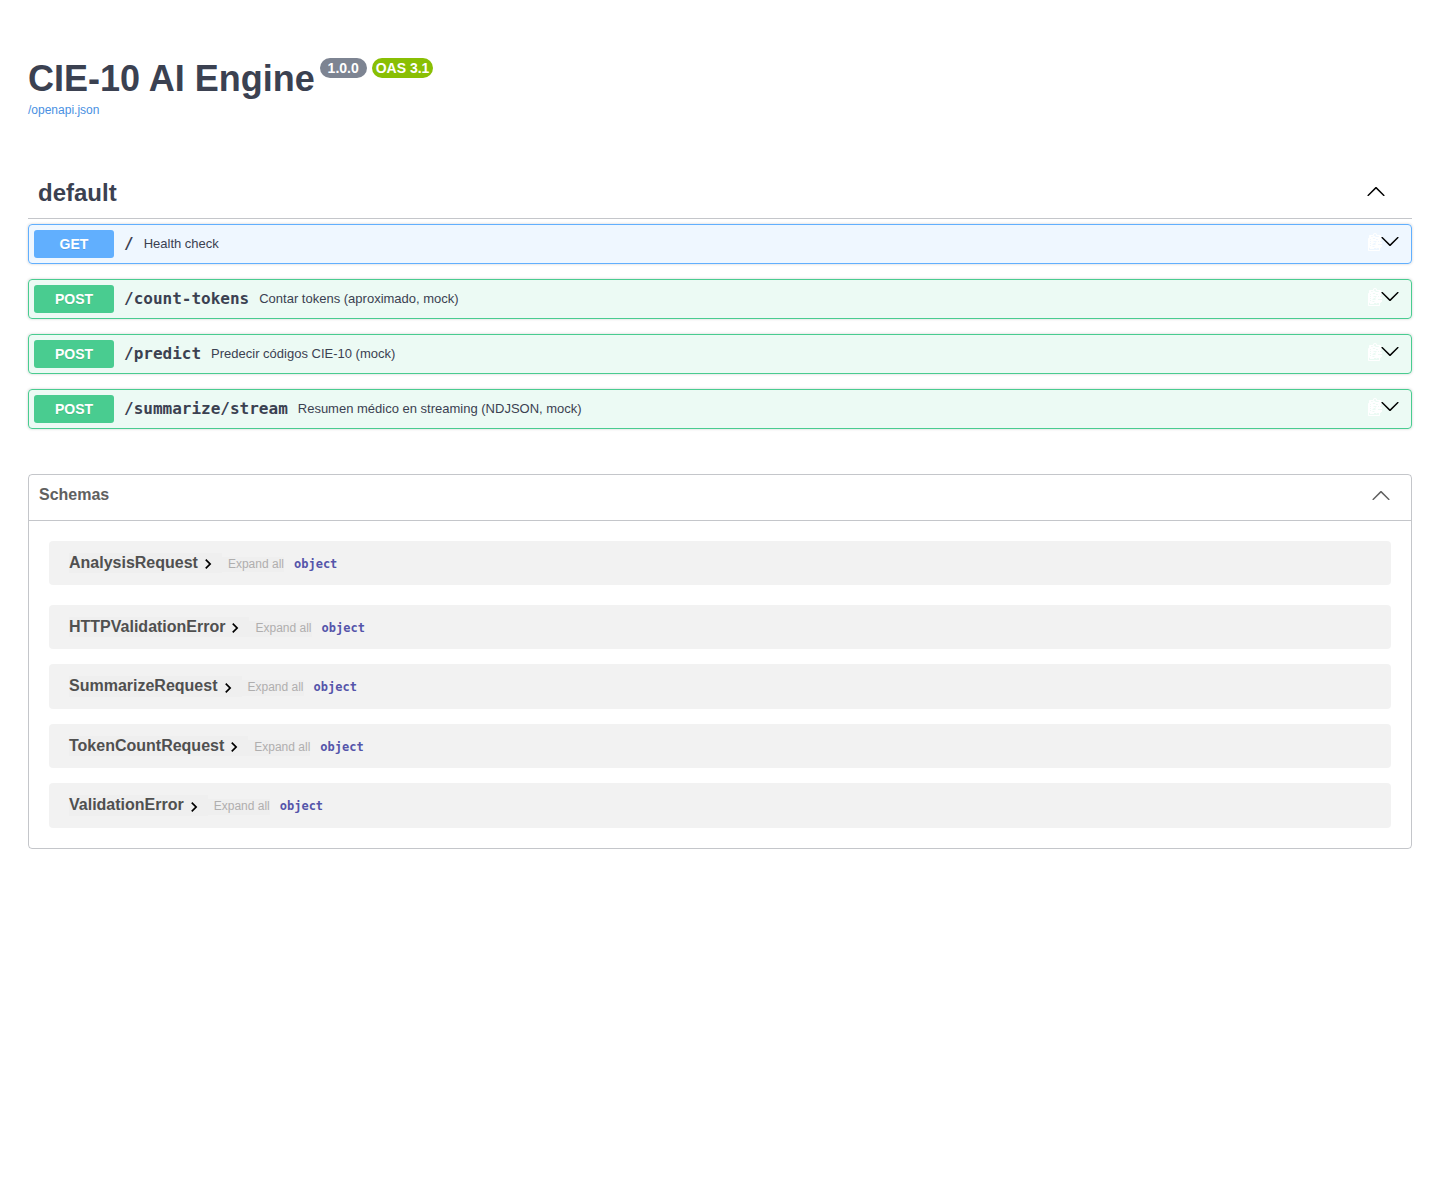
\includegraphics[width=\textwidth]{figs/swagger-ui}
\caption{Swagger UI generada automáticamente por FastAPI para el motor de IA (\texttt{/docs}).}
\label{fig:swagger}
\end{figure}

\paragraph{Obtención en vivo.} Con el sistema en marcha, la especificación completa y siempre actualizada está disponible sin salir del navegador en \texttt{http://localhost:8000/docs} (Swagger UI interactivo) y en \texttt{http://localhost:8000/openapi.json} (esquema OpenAPI 3.1 en JSON, apto para importar en Postman o generar clientes automáticamente). El siguiente fragmento, generado automáticamente por FastAPI, corresponde al \emph{endpoint} \texttt{/predict} y a los esquemas de las dos peticiones que componen un análisis:

{\small
\begin{verbatim}
"/predict": {
 "post": {
 "summary": "Predecir códigos CIE-10",
 "operationId": "predict_codes_predict_post",
 "requestBody": {
 "required": true,
 "content": { "application/json": {
 "schema": { "$ref": "#/components/schemas/AnalysisRequest" } } }
 },
 "responses": {
 "200": { "description": "Successful Response" },
 "422": { "description": "Validation Error", "content": {
 "application/json": { "schema": {
 "$ref": "#/components/schemas/HTTPValidationError" } } } }
 }
 }
}

"AnalysisRequest": {
 "type": "object",
 "required": ["text"],
 "properties": {
 "text": { "type": "string", "title": "Text" },
 "engine": { "type": "string", "title": "Engine", "default": "bert",
 "enum": ["bert", "dict", "both", "fused"] },
 "include_triggers": { "type": "boolean", "title": "Include Triggers",
 "default": false }
 }
}

"ExplainRequest": {
 "type": "object",
 "required": ["text", "codes"],
 "properties": {
 "text": { "type": "string", "title": "Text" },
 "codes": { "type": "array", "items": { "type": "string" },
 "title": "Codes" },
 "method": { "anyOf": [{ "type": "string" }, { "type": "null" }],
 "title": "Method" },
 "top_k": { "type": "integer", "title": "Top K", "default": 5 }
 }
}
\end{verbatim}
}

\section{Endpoints del motor de IA}

La Tabla~\ref{tab:openapi-endpoints} resume los \emph{endpoints} expuestos por el motor de IA.

\begin{table}[h]
\centering
\small
\caption{Endpoints del motor de IA (OpenAPI).}
\label{tab:openapi-endpoints}
\begin{tabular}{llp{7.2cm}}
\hline
\textbf{Método} & \textbf{Ruta} & \textbf{Descripción} \\
\hline
GET & \texttt{/} & Comprobación de estado (\emph{health check}): disponibilidad del servicio y de los modelos. \\
POST & \texttt{/predict} & Predice los códigos CIE-10 de un informe. Parámetro \texttt{engine}: \texttt{bert}, \texttt{dict}, \texttt{both} o \texttt{fused}. \\
POST & \texttt{/explain} & Devuelve los términos que justifican unos códigos ya predichos. \\
POST & \texttt{/count-tokens} & Devuelve el número de \emph{tokens} del texto según el tokenizador del modelo. \\
POST & \texttt{/summarize/stream} & Genera el resumen del informe en \emph{streaming} (NDJSON, token a token). \\
POST & \texttt{/jobs/predict} & Predicción asíncrona: devuelve un \texttt{job\_id} de forma inmediata. \\
POST & \texttt{/jobs/summarize} & Resumen asíncrono: devuelve un \texttt{job\_id} de forma inmediata. \\
GET & \texttt{/jobs/\{job\_id\}} & Consulta el estado y el resultado de un trabajo asíncrono. \\
GET & \texttt{/admin/models} & Lista los modelos publicados y señala cuál está cargado. \\
POST & \texttt{/admin/models} & Carga otro modelo en caliente, sin reiniciar el servicio. \\
POST & \texttt{/admin/summarizer} & Recarga en caliente el modelo de resumen (LLM) y sus \emph{prompts}. \\
GET & \texttt{/metrics} & Métricas en formato Prometheus. \\
\hline
\end{tabular}
\end{table}

\section{Esquemas de petición y respuesta}

\subsection{POST /predict}

Petición:

{\small
\begin{verbatim}
{
 "text": "<informe clínico en español>",
 "engine": "bert" // opcional: "bert" (def.), "dict", "both" o "fused"
}
\end{verbatim}
}

Respuesta: un objeto con el campo \texttt{cards}, que contiene una única tarjeta de tipo \texttt{codes} (el resumen se solicita por separado con \texttt{/summarize/stream}):

{\small
\begin{verbatim}
{
 "cards": [
 {
 "type": "codes",
 "content": [
 {
 "code": "E11.9",
 "description": "Diabetes mellitus tipo 2 sin complicaciones",
 "reason": "Capítulo IV: confianza 91.0%",
 "confidence": 0.91,
 "relative_confidence": 0.86,
 "triggers": ["diabetes", "glucosa"],
 "engine": "bert"
 }
 ]
 }
 ]
}
\end{verbatim}
}

El campo \texttt{confidence} es la probabilidad bruta de la sigmoide; \texttt{relative\_confidence} es su normalización \emph{min-max} dentro del conjunto devuelto (véase la sección~\ref{sec:confianza-predicciones}); \texttt{triggers} son los términos del informe que motivan la predicción (véase la sección~\ref{sec:explicabilidad}); y \texttt{engine} identifica el motor de origen.

\subsection{POST /explain}

La atribución de importancia viaja en un \emph{endpoint} separado porque cuesta del orden de cien veces más que predecir: mide el efecto real de eliminar cada palabra del informe, lo que exige una pasada del \emph{encoder} por palabra. Atarla a \texttt{/predict} obligaba al usuario a esperar por una información que todavía no estaba consultando, ya que primero lee la lista de códigos y solo después despliega uno para saber por qué se ha propuesto. Separadas, los códigos se devuelven en cuanto están y las palabras llegan después.

Por ese motivo \texttt{/predict} admite el campo \texttt{include\_triggers}, desactivado por defecto: activarlo reproduce el comportamiento anterior, en el que la respuesta completa esperaba a la atribución.

La petición indica el texto, los códigos que se quieren justificar y, opcionalmente, la estrategia. La respuesta incluye siempre el método empleado, de modo que ante un término inesperado se puede saber si lo produjo la versión fiel o una de las rápidas (Tabla~\ref{tab:explain-metodos}).

\begin{table}[h]
\centering
\small
\caption{Estrategias de atribución admitidas por \texttt{/explain}.}
\label{tab:explain-metodos}
\begin{tabular}{p{3.3cm}p{9.5cm}}
\hline
\textbf{Método} & \textbf{Descripción} \\
\hline
\texttt{diccionario} & No emplea el \emph{encoder}: devuelve las frases clínicas que hicieron coincidencia por expresión regular. Responde en centésimas de segundo. En el motor fusionado estos términos ya viajan con la predicción sin coste adicional, de modo que esta vía sirve al motor neuronal, que no ejecuta el diccionario. \\
\texttt{gradiente\_filtrado} & Una pasada hacia atrás ordena las palabras candidatas y solo se enmascaran las más prometedoras. \\
\texttt{exhaustivo} & Pregunta por todas las palabras. Es la referencia fiel y la más costosa. \\
\texttt{divide\_y\_venceras} & Enmascara grupos y descarta el que no altera ningún \emph{logit}. Documentado como resultado negativo: en este corpus resulta más lento que el exhaustivo. \\
\hline
\end{tabular}
\end{table}

Los cuatro motores no son variantes del mismo cálculo. \texttt{bert} y \texttt{dict} devuelven las predicciones de un solo clasificador; \texttt{both} devuelve las de ambos concatenadas, cada código con su motor de origen, y deja la reconciliación al cliente; \texttt{fused} combina las puntuaciones de los dos \emph{antes} de ordenar, sumando al \emph{logit} de cada código una bonificación proporcional a la confianza con que el diccionario ha detectado su bloque (Anexo~\ref{cap:AnexoF}, sección~\ref{sec:anexoF-fusion}). Este último emplea un umbral propio, expresado en el espacio de la puntuación combinada, y añade a cada código los campos \texttt{score\_model} y \texttt{score\_dict} con la contribución literal de cada fuente, además de \texttt{dict\_support} y \texttt{trigger\_detail}, que etiqueta cada término explicativo con su procedencia.

\subsection{GET / y POST /count-tokens}

{\small
\begin{verbatim}
GET / -> {"status": "online", "model_loaded": true,
 "dict_loaded": true, "summarizer_loaded": true, ...}

POST /count-tokens {"text": "..."} -> {"token_count": 349}
\end{verbatim}
}

\section{Streaming NDJSON: \texttt{POST /summarize/stream}}

El resumen del informe se entrega mediante \textbf{NDJSON} (\emph{newline-delimited JSON}): la respuesta es un flujo en el que \textbf{cada línea es un objeto JSON independiente}, lo que permite al cliente renderizar el texto de forma incremental (efecto \emph{typewriter}) sin esperar a que el LLM termine. El tipo de contenido de la respuesta es \texttt{application/x-ndjson}.

El protocolo es el siguiente: se emite una línea por cada fragmento generado y una línea final que señala el fin del flujo; ante un error se emite una línea de error antes de cerrar.

{\small
\begin{verbatim}
{"token": "Paciente "}
{"token": "de 70 "}
{"token": "años con "}
...
{"done": true}
\end{verbatim}
}

En caso de fallo del generador, la última línea es \texttt{\{"error": "<mensaje>"\}} en lugar de \texttt{\{"done": true\}}. Si el modelo de resumen no está cargado, el servicio devuelve un único fragmento con un resumen estadístico de reserva y a continuación \texttt{\{"done": true\}}, de modo que el cliente siempre recibe una respuesta bien formada.

El backend retransmite cada línea recibida al frontend a través del canal WebSocket como eventos \texttt{summary\_token} (véase el Anexo~\ref{cap:AnexoC}), desacoplando así el protocolo interno (NDJSON) del protocolo con el cliente (WebSocket).
 % Anexo M: Especificación de la API (OpenAPI + NDJSON)
%--- (FIN DOCUMENTO)
\end{document}